\clearpage
\bookpart{随机优化}{Stochastic Optimization}
\label{part:stochastic-optimization}

\BookPartGuide{%
前面的方法都假定能读到准确的目标值和梯度。实际问题中常常只能读到一部分数据上的梯度、带噪声的函数值，甚至只知道评价一次很昂贵。本部分按可取得的信息和更新方式划分四章。

第~\ref{chap:stochastic-gradient-methods}章使用随机梯度：每步只读取部分目标项，用较低的单步代价换来有噪声的方向，再通过步长、方差控制、动量和自适应缩放控制误差。第~\ref{chap:zeroth-order-optimization}章只能读取函数值，用扰动和差分构造局部方向。第~\ref{chap:random-search}章放弃局部方向，通过随机提议、群体变异和历史记忆探索解空间。第~\ref{chap:bayesian-optimization}章面向每次评价都昂贵的黑箱问题，用概率模型总结已有观测，再决定下一个评价点。

“随机”在这四章里含义不同：可能是算法抽样的随机，可能是函数值中的噪声，也可能只是用概率描述我们对未知函数的了解。各章在开头分别说明，不混用。}

\chapter{随机梯度方法}
\label{chap:stochastic-gradient-methods}

要拟合一百万条观测，目标是每条观测上误差的平均。梯度下降每走一步，都要把一百万条观测读一遍，只为知道下山的方向。可是这个方向本身只是一个平均值，而估计平均值并不需要读完全部数据：问几个人，就能大致知道全校的平均身高。于是有了本章的想法：每一步只读一小部分目标项，用它代替完整梯度。

这个想法马上带来几个问题。只读一项得到的方向可能是错的，甚至指向上山，那么算法凭什么收敛？读数的抖动在最优点附近也不停止，迭代点最后会停在哪里，步长应该怎样选？既然噪声是麻烦，能不能设法把它压下去，压下去又要花多少代价？

本章按这样的路线回答。先固定要最小化的目标，说清一个随机向量什么时候算作当前梯度的估计，再把它代入更新，建立有限步的误差界，并比较返回哪个点。然后研究怎样减小估计的误差。此后转向另一类做法：不改变读取的对象，而改变读数被使用的方式，包括累积历史方向、按坐标调整尺度和事先处理梯度。最后回到原目标，比较误差和总计算量。

全章用同一个三项一元二次目标做例子。它小到可以手算，每一项的梯度又足够不同，读一项和读全部的差别看得很清楚。

\section{随机目标与梯度估计}
\label{sec:sgd-objectives}

只读部分信息时，手里得到的向量和当前点的真梯度是什么关系？回答它需要先说清要最小化的是哪个目标，再说清“随机”来自哪里，最后给出“这个读数可以当作梯度用”的准确含义。读取的顺序也会改变这一含义，放在本节最后讨论。

\subsection{有限和目标}
\label{sec:sgd-finite-sum}

先看最常见的情形：数据已经固定，目标是$N$项的平均。

\paragraph{目标与完整梯度}
设$f_i:\mathbb{R}^n\to\mathbb{R}$，$i=1,\ldots,N$，都可微。\term{有限和目标}（finite-sum objective）是
\begin{equation}
 f(\bm{x})=\frac{1}{N}\sum_{i=1}^{N}f_i(\bm{x}).
 \label{eq:sgd-finite-sum}
\end{equation}
求导对有限和可以逐项进行，所以完整梯度是各项梯度的平均：
\begin{equation}
 \nabla f(\bm{x})=\frac{1}{N}\sum_{i=1}^{N}\nabla f_i(\bm{x}).
 \label{eq:sgd-full-gradient}
\end{equation}
要得到它，必须把$N$项都计算一遍。本章把计算一项梯度称为一次\emph{读取}，完整梯度的代价是$N$次读取。

\paragraph{均匀抽取一项}
现在换一种获取信息的方式：在$\{1,\ldots,N\}$中均匀抽一个下标$i$，只计算$\nabla f_i(\bm{x})$。每个下标的概率都是$1/N$，因此对这次抽样求平均，得到
\begin{equation}
 \mathbb{E}_i[\nabla f_i(\bm{x})]=\sum_{i=1}^{N}\frac{1}{N}\nabla f_i(\bm{x})=\nabla f(\bm{x}).
 \label{eq:sgd-uniform-mean}
\end{equation}
目标函数并没有变，变的只是当前拿到的信息：从全部$N$项变成其中一项。

这就像估计全校的平均身高：不必量遍每个人，随机问一个人，他的身高在平均意义上就是全校的平均。学生对应目标项，身高对应该项的梯度，全校平均对应完整梯度。这个类比有两处失效。身高不随时间改变，而$\nabla f_i(\bm{x})$随$\bm{x}$改变，每走一步都要重新估计。另外，估计身高只要结果，估计梯度还要照着它走路，走错的后果会带到下一步。

\paragraph{贯穿全章的三项目标}
取一元、三项的目标，每项是一条抛物线：
\begin{equation}
 f_i(x)=\frac{a_i}{2}(x-b_i)^2,\qquad
 (a_1,a_2,a_3)=(1,2,3),\qquad
 (b_1,b_2,b_3)=(-3,0,3).
 \label{eq:sgd-example-terms}
\end{equation}
三项写出来是
\[
 f_1(x)=\frac12(x+3)^2,\qquad f_2(x)=x^2,\qquad f_3(x)=\frac32(x-3)^2.
\]

把三项相加再除以$3$。二次项系数是$\tfrac16+\tfrac13+\tfrac12=1$，一次项系数是$1+0-3=-2$，常数项是$\tfrac32+0+\tfrac92=6$，所以
\begin{equation}
 f(x)=x^2-2x+6=(x-1)^2+5.
 \label{eq:sgd-example-objective}
\end{equation}
于是最小点和最优值是
\[
 x^\star=1,\qquad f^\star=5.
\]

各项的梯度$f_i'(x)=a_i(x-b_i)$与完整梯度是
\begin{equation}
 f_1'(x)=x+3,\qquad f_2'(x)=2x,\qquad f_3'(x)=3x-9,\qquad f'(x)=2x-2.
 \label{eq:sgd-example-gradients}
\end{equation}
这里$f$的曲率是$2$，所以$L=\mu=2$；各项自身的曲率是$L_i=a_i$，最大为$3$。

在$x=2$处，三项的读数和完整梯度是
\[
 f_1'(2)=5,\qquad f_2'(2)=4,\qquad f_3'(2)=-3,\qquad f'(2)=2.
\]
第三项的读数是负的，说明它主张向右走，而完整梯度要求向左走。最优点$x^\star=1$恰在左边，听第三项的话就走反了。在最优点，三项读数为$(4,2,-6)$，它们的和是零，但没有一项是零。完整梯度已经停下，单项读数并没有停下。这两个现象会贯穿全章。

\begin{BookInlineFigure}
  \centering
  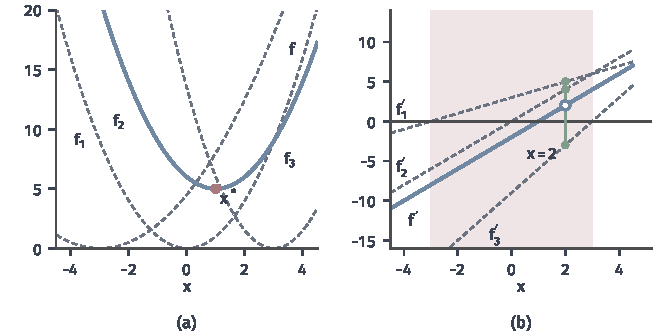
\includegraphics[width=112mm]{figures/05-optimization/05-stochastic-optimization/matplotlib/sgd-term-gradients/figure.pdf}
  \caption{三项目标~\eqref{eq:sgd-example-terms}。(a)虚线是三条单项抛物线$f_1,f_2,f_3$，实线是它们的平均$f$，红点是$f$的最小点$x^\star=1$，各项的最小点都不在这里。(b)虚线是单项导数，实线是$f'$。红底区间$[-3,3]$内三项导数不同号；区间外三项同号，都指向区间。竖线段标出$x=2$处的三个读数$5,4,-3$，空心点是它们的平均$2$。}
  \label{fig:sgd-term-gradients}
\end{BookInlineFigure}

图~\ref{fig:sgd-term-gradients}(b)给出了分歧发生的位置。三条单项导数的零点是$-3,0,3$，在这三个数之外，三项一致地指向同一边，读哪一项方向都对。进入$[-3,3]$后各项开始争执。所以离解还远时，单项读数和完整梯度方向相同；离解越近，分歧越明显。

\paragraph{归一化、正则项与读取成本}
式~\eqref{eq:sgd-finite-sum}里的$1/N$不是可有可无的约定。若目标写成不除以$N$的总和，最小点不变，但梯度和光滑常数都放大$N$倍，同一个数值的步长含义完全不同。本章一律使用平均的写法，步长$\alpha$可以脱离$N$来讨论。

许多目标还带确定的正则项$r$，例如$r(\bm{x})=\tfrac{\gamma}{2}\lVert\bm{x}\rVert_2^2$：
\begin{equation}
 f(\bm{x})=\frac{1}{N}\sum_{i=1}^{N}f_i(\bm{x})+r(\bm{x}).
 \label{eq:sgd-finite-sum-regularized}
\end{equation}
$r$不依赖数据项，它的梯度每步都能精确算出，无需抽样。读数应写成$\nabla f_i(\bm{x})+\nabla r(\bm{x})$。如果把$r$放进每一项，写成$f_i+r$，结果相同；要避免的是只在抽到某些项时才加入$r$，或把系数随$N$改变而不作说明。

计数时要分清两种成本：一次读取是对单项的梯度计算，一次更新是对$\bm{x}$的修改。完整梯度下降每次更新$N$次读取，只读一项时每次更新一次读取。比较算法时，本章以读取次数为主要的计量单位。

\subsection{期望目标}
\label{sec:sgd-expected}

很多问题中项数不是固定的$N$。观测可以源源不断地取得，或者目标本来就是在某个分布上的平均。

\paragraph{从有限平均到期望}
设$\bm{\xi}$是可以抽样的随机变量，对每个$\bm{\xi}$的取值有函数$\phi(\bm{x};\bm{\xi})$。\term{期望目标}（expected objective）是
\begin{equation}
 f(\bm{x})=\mathbb{E}_{\bm{\xi}}[\phi(\bm{x};\bm{\xi})].
 \label{eq:sgd-expected-objective}
\end{equation}
有限和是特例：取$\bm{\xi}$为均匀分布的下标$i$，$\phi(\bm{x};i)=f_i(\bm{x})$。三项目标正是这样，$f$是三点分布上的期望。

一般情况下无法把所有取值列出来，也无法求出$f$，却能抽样。这样就有两种不同的做法。

一种是\emph{直接优化期望}：每一步抽一个新样本，把它的梯度用于更新。每个样本只用一次，读取总数等于样本总数，要最小化的始终是式~\eqref{eq:sgd-expected-objective}。另一种是\emph{先固定一批样本}：一次抽定$\bm{\xi}_1,\ldots,\bm{\xi}_N$，得到
\[
 f_N(\bm{x})=\frac{1}{N}\sum_{i=1}^{N}\phi(\bm{x};\bm{\xi}_i),
\]
然后把$f_N$当作有限和目标反复读取。这时算法解的是$f_N$，它的解一般不是$f$的解。

\begin{BookInlineFigure}
  \centering
  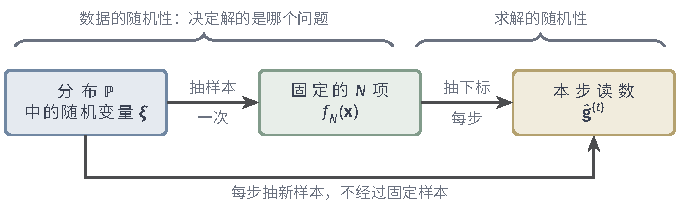
\includegraphics[width=112mm]{figures/05-optimization/05-stochastic-optimization/tikz/sgd-two-randomness/figure.pdf}
  \caption{两层随机性。上方路线先抽定$N$个样本，得到确定的有限和$f_N$，之后每步只对下标抽样。下方路线不经过固定样本，每步直接抽新样本。第一层随机性决定了算法解的是哪个问题，第二层只影响算法解这个问题的过程。}
  \label{fig:sgd-two-randomness}
\end{BookInlineFigure}

图~\ref{fig:sgd-two-randomness}区分了这两层随机性。举一个具体的例子：取$\phi(x;\xi)=\tfrac12(x-\xi)^2$，$\xi$的均值为$1$。期望目标的最小点是$1$，而$f_N$的最小点是样本均值$\bar{\xi}_N$，它随样本变化。无论优化做得多准，都只能精确得到$\bar{\xi}_N$；$\bar{\xi}_N$与$1$的差属于数据造成的统计误差。本章固定目标，只研究优化误差。统计误差的大小可参考\BookChapterRef{chap:finite-sample-error-bounds}{卷八第4章“有限样本的误差上界”}。

\paragraph{逐样本求导的条件}
随机梯度要求$\nabla\phi(\bm{x};\bm{\xi})$的期望等于$\nabla f(\bm{x})$，也就是导数和期望可以交换。有限和中这一步只是有限项相加，期望的情形需要条件。

\begin{lemma}[逐样本求导]
\label{lem:sgd-differentiate-expectation}
设$\bm{x}$有开球邻域$\bm{U}$，$\phi(\bm{x};\bm{\xi})$可积。若几乎所有$\bm{\xi}$使$\phi(\cdot;\bm{\xi})$在$\bm{U}$上可微，且存在可积函数$M(\bm{\xi})$，使
\begin{equation}
 \lVert\nabla\phi(\bm{y};\bm{\xi})\rVert_2\leq M(\bm{\xi}),\qquad \bm{y}\in\bm{U},
 \label{eq:sgd-local-domination}
\end{equation}
则$f$在$\bm{x}$处可微，并且
\begin{equation}
 \nabla f(\bm{x})=\mathbb{E}_{\bm{\xi}}[\nabla\phi(\bm{x};\bm{\xi})].
 \label{eq:sgd-gradient-expectation}
\end{equation}
\end{lemma}

\begin{proof}
记$\bm{v}(\bm{\xi})=\nabla\phi(\bm{x};\bm{\xi})$。由式~\eqref{eq:sgd-local-domination}，$\bm{v}$可积。取$\bm{h}^{(k)}\to\bm{0}$，$\bm{h}^{(k)}\neq\bm{0}$，且$\bm{x}+\bm{h}^{(k)}\in\bm{U}$，令
\[
 R_k(\bm{\xi})=\frac{\phi(\bm{x}+\bm{h}^{(k)};\bm{\xi})-\phi(\bm{x};\bm{\xi})-\langle\bm{v}(\bm{\xi}),\bm{h}^{(k)}\rangle}{\lVert\bm{h}^{(k)}\rVert_2}.
\]

对几乎所有$\bm{\xi}$，由可微性有$R_k(\bm{\xi})\to0$。沿线段使用中值定理，并由式~\eqref{eq:sgd-local-domination}，得到
\[
 \lvert R_k(\bm{\xi})\rvert\leq2M(\bm{\xi}).
\]
这说明$\phi(\bm{x}+\bm{h}^{(k)};\cdot)$也可积，$f$在这些点有定义。

控制收敛定理给出$\mathbb{E}[R_k]\to0$，定理的条件和证明见\BookChapterRef{chap:integration}{卷四第6章“积分”}。序列$\bm{h}^{(k)}$是任取的，所以这正是$f$在$\bm{x}$处以$\mathbb{E}[\bm{v}]$为梯度可微的定义。
\end{proof}

条件~\eqref{eq:sgd-local-domination}去掉后结论可以错得很彻底。取$\xi$在$(0,1)$上均匀，$\phi(x;\xi)$是示性函数：当$\xi\leq x$时取$1$，否则取$0$。对$x\in(0,1)$，期望目标是$f(x)=x$，导数处处为$1$。但对每个固定的$\xi$，除$x=\xi$这一点外函数都是常数，逐样本导数是$0$，平均之后还是$0$。跳跃点带来的贡献被逐样本求导完全漏掉了。对照引理的条件，落在$\bm{U}$内的$\xi$使$\phi(\cdot;\xi)$在$y=\xi$处不连续，“在整个邻域上可微”这一条不成立；只在$x$这一点几乎处处可微是不够的。

分布本身依赖$\bm{x}$时，式~\eqref{eq:sgd-gradient-expectation}不能直接用，因为抽样分布也在变。常用的处理是把随机性移到不依赖$\bm{x}$的变量上（重参数化），或用分布密度的对数导数作权重（得分函数估计），可参考\BookChapterRef{chap:expectation-gradient-estimation}{卷七第33章“含参期望的梯度估计”}。本章下文只讨论分布不依赖$\bm{x}$的情形。

\subsection{条件无偏与读数误差}
\label{sec:sgd-unbiased}

式~\eqref{eq:sgd-uniform-mean}是对固定的$\bm{x}$写的。迭代中$\bm{x}^{(t)}$本身由前面的抽样决定，也是随机的。需要一个能处理“当前点已经随机地到了这里”的说法。

\paragraph{历史与条件期望}
把第$t$步抽样之前已经发生的一切称为\emph{历史}，记为$\mathcal{F}^{(t)}$：初始点、前$t$次抽到的下标。给定历史，$\bm{x}^{(t)}$就是一个确定的点。条件期望$\mathbb{E}[\cdot\mid\mathcal{F}^{(t)}]$可以这样理解：把过去冻结，只对第$t$步的新抽样求平均。

本章反复使用条件期望的两条规则。历史已知的量可以提到条件期望外面：
\begin{equation}
 \mathbb{E}[\,\bm{u}^\top\bm{v}\mid\mathcal{F}^{(t)}]=\bm{u}^\top\mathbb{E}[\bm{v}\mid\mathcal{F}^{(t)}],\qquad \bm{u}\text{由}\mathcal{F}^{(t)}\text{确定}.
 \label{eq:sgd-pull-out}
\end{equation}
先对新抽样平均、再对历史平均，等于直接取总平均，即全期望公式：
\begin{equation}
 \mathbb{E}\bigl[\mathbb{E}[X\mid\mathcal{F}^{(t)}]\bigr]=\mathbb{E}[X].
 \label{eq:sgd-tower}
\end{equation}
这两条规则的一般表述和条件可参考\BookChapterRef{chap:conditional-expectation}{卷七第10章“条件期望”}。

下面把读数记作$\hat{\bm{g}}^{(t)}$，$\bm{g}^{(t)}=\nabla f(\bm{x}^{(t)})$仍表示真梯度。

\begin{definition}[条件无偏]
\label{def:sgd-unbiased}
若随机向量$\hat{\bm{g}}^{(t)}$满足
\begin{equation}
 \mathbb{E}[\hat{\bm{g}}^{(t)}\mid\mathcal{F}^{(t)}]=\nabla f(\bm{x}^{(t)}),
 \label{eq:sgd-unbiased}
\end{equation}
就称它是当前梯度的\term{条件无偏}（conditionally unbiased）估计。
\end{definition}

条件不能换成不带条件的$\mathbb{E}[\hat{\bm{g}}^{(t)}]$。在三项目标上从$x^{(0)}=2$出发，取$\alpha=0.1$。第一步的三种可能是$x^{(1)}=1.5,1.6,2.3$。若第一步抽到第三项，给定这段历史后当前点是$2.3$，第二步读数的条件均值是
\[
 \mathbb{E}[\hat{g}^{(1)}\mid\mathcal{F}^{(1)}]=f'(2.3)=2.6.
\]
不带条件地平均，则要把三种历史也平均进去，得到的是
\[
 \mathbb{E}[\hat{g}^{(1)}]=\frac{f'(1.5)+f'(1.6)+f'(2.3)}{3}=1.6.
\]
算法站在$2.3$处需要的是$2.6$这个数，$1.6$回答的是另一个问题。

\paragraph{读数的分解}
一般的读数未必无偏。把它分成三部分来记录：
\begin{equation}
 \hat{\bm{g}}^{(t)}=\nabla f(\bm{x}^{(t)})+\bm{b}^{(t)}+\bm{\zeta}^{(t)},
 \label{eq:sgd-read-decomposition}
\end{equation}
其中条件偏差和零条件均值噪声分别是
\[
 \bm{b}^{(t)}=\mathbb{E}[\hat{\bm{g}}^{(t)}\mid\mathcal{F}^{(t)}]-\nabla f(\bm{x}^{(t)}),\qquad
 \bm{\zeta}^{(t)}=\hat{\bm{g}}^{(t)}-\mathbb{E}[\hat{\bm{g}}^{(t)}\mid\mathcal{F}^{(t)}].
\]

\begin{BookInlineFigure}
  \centering
  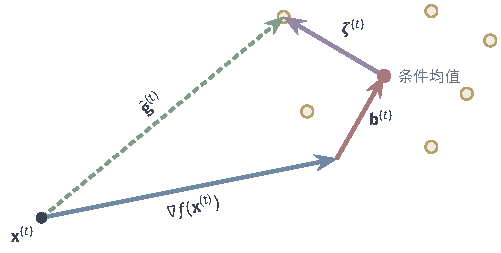
\includegraphics[width=80mm]{figures/05-optimization/05-stochastic-optimization/tikz/sgd-read-decomposition/figure.pdf}
  \caption{读数的三段分解。蓝色是真梯度，红色是条件偏差，紫色是一次读数偏离条件均值的噪声，绿色虚线是最终拿到的读数。黄色小圆是其他可能的读数，它们围绕条件均值分布。条件无偏的含义是红色线段长度为零，黄色小圆的中心落在蓝色箭头的端点上。}
  \label{fig:sgd-read-decomposition}
\end{BookInlineFigure}

图~\ref{fig:sgd-read-decomposition}说明了两部分误差的不同性质。偏差是系统性的，反复平均也去不掉；噪声的均值为零，累积时会相互抵消一部分。在二阶量上这个区别体现为交叉项消失。噪声的条件均值为零，再由规则~\eqref{eq:sgd-pull-out}，交叉项为零，于是
\begin{equation}
 \mathbb{E}[\lVert\hat{\bm{g}}^{(t)}\rVert_2^2\mid\mathcal{F}^{(t)}]
 =\lVert\nabla f(\bm{x}^{(t)})+\bm{b}^{(t)}\rVert_2^2+\mathbb{E}[\lVert\bm{\zeta}^{(t)}\rVert_2^2\mid\mathcal{F}^{(t)}].
 \label{eq:sgd-second-moment}
\end{equation}
后面的分析分别记录这两个量，噪声的条件二阶矩也称条件方差。

\paragraph{例中的偏差与方差}
三项目标上均匀抽样的读数无偏，$\bm{b}^{(t)}=0$。令$\delta=x-1$，式~\eqref{eq:sgd-example-gradients}的三个读数写成$\delta+4$，$2\delta+2$，$3\delta-6$。它们平方的平均是
\[
 \frac13\bigl[(\delta+4)^2+(2\delta+2)^2+(3\delta-6)^2\bigr]=\frac{14\delta^2-20\delta+56}{3}.
\]
减去$f'(x)^2=4\delta^2$，得到条件方差
\begin{equation}
 \sigma^2(x)=\frac{2\delta^2-20\delta+56}{3},\qquad \delta=x-1.
 \label{eq:sgd-example-variance}
\end{equation}
在$x=x^\star$处它等于$56/3\approx18.67$，这时完整梯度已经是零，噪声却最明显。在$x=2$处，$\delta=1$，方差是$38/3\approx12.67$。

式~\eqref{eq:sgd-example-variance}还说明，方差随$\lvert x\rvert\to\infty$按$\delta^2$增长。“条件方差处处不超过某个常数”这种常用假设，即使对最简单的二次目标也只在有界区域内成立。下文使用这类假设时，都理解为沿迭代点成立，它通常需要迭代点停留在有界区域内，这件事本身需要验证。

有偏的读数也容易构造。若按概率$(1/2,1/4,1/4)$抽项，又直接使用读数而不作修正，$x=2$处的条件均值是
\[
 \frac12\cdot5+\frac14\cdot4+\frac14\cdot(-3)=2.75,
\]
相对$f'(2)=2$的偏差是$0.75$。第~\ref{sec:sgd-importance}小节将说明这种偏差怎样改变实际求解的目标，以及如何用权重把它去掉。

\paragraph{无偏不保证单步下降}
条件无偏是平均意义上的性质，一次读数可能与真梯度成钝角。$x=2$处抽到第三项时，读数$-3$和真梯度$2$的乘积是$-6$，沿负读数走一步函数值上升。对比之下，条件无偏只保证
\[
 \mathbb{E}[\langle\nabla f(\bm{x}^{(t)}),\hat{\bm{g}}^{(t)}\rangle\mid\mathcal{F}^{(t)}]=\lVert\nabla f(\bm{x}^{(t)})\rVert_2^2\geq0.
\]
所以随机梯度方法不能用“每步函数值都下降”来分析，要用的是期望意义上的进展。

\subsection{循环读取与随机重排}
\label{sec:sgd-reading-orders}

上面的条件无偏依赖每步独立抽样。可在有限和目标上，常见的读取方式并不独立。

\paragraph{三种读取顺序}
有放回抽样每步独立地均匀抽一个下标，这一轮里有的项可能抽到多次，有的项可能一次也没抽到。固定循环按$1,2,\ldots,N$的顺序反复读取。\term{随机重排}（random reshuffling）每轮开始时把$N$项随机打乱一次，然后无放回地读完。把连续读取$N$项称为一\emph{轮}，后两种方式的每一轮都恰好读全部的项，图~\ref{fig:sgd-reading-orders}对比了三种方式。

\begin{BookInlineFigure}
  \centering
  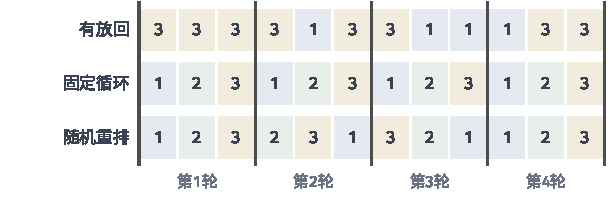
\includegraphics[width=104mm]{figures/05-optimization/05-stochastic-optimization/matplotlib/sgd-reading-orders/figure.pdf}
  \caption{三项目标在四轮内的读取顺序（种子固定）。每格的数字和底色表示读到的项，粗竖线分隔各轮。有放回抽样的一轮可能缺项、重项，固定循环每轮相同，随机重排每轮恰好各读一次，但顺序每轮不同。}
  \label{fig:sgd-reading-orders}
\end{BookInlineFigure}

\paragraph{一轮之内读数有偏}
随机重排打破了逐步条件无偏。在$x=2$处，设本轮首先读了第三项。给定这段历史，剩下两项的读数是第一项和第二项，平均后是
\[
 \frac{f_1'(2)+f_2'(2)}{2}=\frac{5+4}{2}=4.5.
\]
而完整梯度是$2$。这个偏差很好理解：读了负的一项，剩下的项一定偏正。所以式~\eqref{eq:sgd-unbiased}对随机重排的一轮内部不成立，无法直接沿用逐步的条件期望递推。

\paragraph{按整轮来分析}
偏差并不是坏事，因为一轮的总和是精确的。把一轮的$N$项读取顺序记为$\pi_0,\ldots,\pi_{N-1}$，轮内迭代点记为$\bm{x}_0,\ldots,\bm{x}_N$，步长固定为$\alpha$。把每一步的读数在轮初的点$\bm{x}_0$处展开，
\[
 \bm{x}_N=\bm{x}_0-\alpha\sum_{k=0}^{N-1}\nabla f_{\pi_k}(\bm{x}_k).
\]
一轮恰好读全部的项，所以各项读数在同一点$\bm{x}_0$处的和就是$N$倍的完整梯度。在每一项里加减$\nabla f_{\pi_k}(\bm{x}_0)$，得到
\begin{equation}
 \bm{x}_N=\bm{x}_0-\alpha N\nabla f(\bm{x}_0)-\alpha\sum_{k=0}^{N-1}\bigl[\nabla f_{\pi_k}(\bm{x}_k)-\nabla f_{\pi_k}(\bm{x}_0)\bigr].
 \label{eq:sgd-epoch-expansion}
\end{equation}
第一部分恰是步长$\alpha N$的一次完整梯度下降，与顺序无关。若各项梯度$L_i$-Lipschitz，第二部分的每一项不超过$L_i\lVert\bm{x}_k-\bm{x}_0\rVert_2$，而$\lVert\bm{x}_k-\bm{x}_0\rVert_2$本身是$\alpha$的量级，所以这部分是$\alpha^2$的量级。

一轮之内读到的梯度并不消失，它们的噪声在一轮结束时几乎抵消。有放回抽样没有这个结构，每步噪声$\alpha\bm{\zeta}^{(t)}$是$\alpha$的量级，一轮的总噪声还是$\alpha$的量级。

三项目标可以直接核对。从$x_0=2$开始，步长$\alpha=0.1$，顺序为$3,1,2$，轮内的点依次是$2.3,\ 1.77,\ 1.416$。式~\eqref{eq:sgd-epoch-expansion}的第一部分给出
\[
 2-0.1\cdot3\cdot2=1.4.
\]
第二部分的三项里，第三项在$x_0$处读取，差为零；第一项在$2.3$处读取，差是$1\cdot0.3$；第二项在$1.77$处读取，差是$2\cdot(-0.23)$。所以第二部分是
\[
 -0.1\cdot(0+0.3-0.46)=0.016,
\]
两部分合计$1.416$，与逐步计算一致。

\begin{BookInlineFigure}
  \centering
  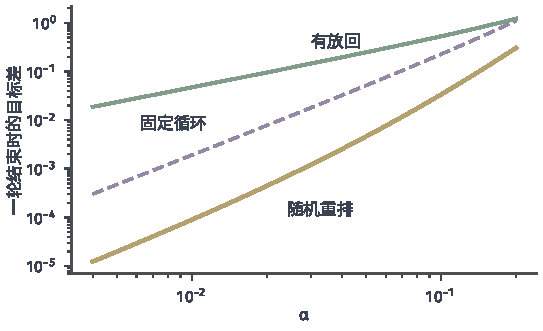
\includegraphics[width=92mm]{figures/05-optimization/05-stochastic-optimization/matplotlib/sgd-epoch-floor/figure.pdf}
  \caption{三项目标上固定步长运行至稳定后，一轮结束时的期望目标差与步长的关系，两轴都取对数。数值由精确递推算出，并非抽样估计。绿线是有放回抽样，紫色虚线是固定顺序$1,2,3$，黄线是随机重排。}
  \label{fig:sgd-epoch-floor}
\end{BookInlineFigure}

图~\ref{fig:sgd-epoch-floor}比较了固定步长长期运行后的误差。图中的三条直线斜率不同：步长缩小十倍时，有放回抽样的目标差约缩小十倍；固定循环约缩小一百倍；随机重排缩小的倍数更大，在$\alpha=0.1$和$0.01$之间约为三百七十倍，曲线向千倍的斜率靠近。在$\alpha=0.01$时，三者的目标差依次约为$4.7\times10^{-2}$，$1.9\times10^{-3}$，$9.0\times10^{-5}$。

固定循环的误差是一个确定的偏移，步长固定后迭代点按周期收敛到一条轨道，其离$x^\star$的距离是$\alpha$的量级，目标差是$\alpha^2$的量级，而且偏移大小与读取顺序有关。随机重排把各种顺序平均，轮末偏移的主要部分相互抵消。

这张图只来自一个二次例子，斜率不能直接当作一般定理。一般目标上，随机重排的结论需要对一轮的累积偏差单独分析，证明较长，读者可查阅相关文献。本章后面的逐步分析都针对有放回抽样或新样本的情形，把它们用于随机重排时要注意上面的差别。

\section{随机梯度方法}
\label{sec:sgd-method}

上一节说清了读数和真梯度的关系。这就需要回答：把读数直接放进梯度更新后，有限步之内能保证什么？答案由三件事决定：抽样和步长的先后，步长的大小随时间怎样变化，以及最后返回哪个点。

\subsection{随机梯度下降}
\label{sec:sgd-basic}

\paragraph{主要思想}
把梯度下降式中的$\nabla f(\bm{x}^{(t)})$换成读数，就得到\term{随机梯度下降}（stochastic gradient descent）：
\begin{equation}
 \begin{gathered}
 \bm{x}^{(t+1)}=\bm{x}^{(t)}-\alpha^{(t)}\hat{\bm{g}}^{(t)},\\
 \hat{\bm{g}}^{(t)}=\nabla f_{i^{(t)}}(\bm{x}^{(t)}).
 \end{gathered}
 \label{eq:sgd-update}
\end{equation}
$i^{(t)}$是第$t$步抽到的下标，对期望目标则换成新样本$\bm{\xi}^{(t)}$。

可以把它想成下山时每一步只问一位向导。每位向导都有自己的偏好，单独听一位可能走错，但向导们的平均意见是对的。步子小时，连走许多步的总位移接近多位意见的累积，错误相互抵消，走的是平均路线。这个类比说明步长必须小：步子大时一次错误就走出很远，后面来不及纠正。

式~\eqref{eq:sgd-update}的执行顺序有讲究。基本分析要求$\alpha^{(t)}$在抽取$i^{(t)}$之前已经确定，也就是$\alpha^{(t)}$由历史$\mathcal{F}^{(t)}$决定。这样在条件期望中它可以提到外面，式~\eqref{eq:sgd-pull-out}才能用。

\needspace{6\baselineskip}
\paragraph{变量}
\begin{itemize}
 \item $\bm{x}^{(t)}\in\mathbb{R}^n$：当前点，在原处更新。
 \item $i^{(t)}$：本步抽到的下标，用完即弃。
 \item $\hat{\bm{g}}^{(t)}\in\mathbb{R}^n$：本步读数。
 \item $\alpha^{(t)}>0$：本步步长，抽样前确定。
 \item $\hat{\bm{x}}$：最后返回的点，是最后一个迭代点还是某种平均，后面讨论。
\end{itemize}

\paragraph{初始化}
选定初始点、步长规则和总步数$T$。例中取
\[
 x^{(0)}=2,\qquad \alpha=0.1,
\]
并设前三步抽到的下标依次是$3,1,2$。

\paragraph{每轮更新}
对$t=0,1,\ldots,T-1$依次执行以下步骤。

\begin{enumerate}
 \item 抽样：独立地均匀抽取下标$i^{(t)}$。例中第一轮$i^{(0)}=3$。
 \item 读取：计算本项在当前点的梯度，作为读数$\hat{\bm{g}}^{(t)}$。例中第一轮由式~\eqref{eq:sgd-example-gradients}，
 \[
  \hat{g}^{(0)}=3\cdot2-9=-3.
 \]
 \item 更新：由式~\eqref{eq:sgd-update}计算新点。例中第一轮
 \[
  x^{(1)}=2-0.1\cdot(-3)=2.3.
 \]
 目标差从$1$变成$1.69$，这一步走了上坡。
 \item 记录：保存计算输出所需的量。若返回平均点，这里累加$\alpha^{(t)}\bm{x}^{(t)}$和$\alpha^{(t)}$；例中只保留当前点。
\end{enumerate}

例中第二轮$i^{(1)}=1$，读数和新点是
\[
 \hat{g}^{(1)}=2.3+3=5.3,\qquad x^{(2)}=2.3-0.53=1.77.
\]

例中第三轮$i^{(2)}=2$，读数和新点是
\[
 \hat{g}^{(2)}=2\cdot1.77=3.54,\qquad x^{(3)}=1.77-0.354=1.416.
\]

迭代在预定的$T$步后结束。随机梯度不能用$\lVert\hat{\bm{g}}^{(t)}\rVert_2$作停止判据，因为它在最优点也不趋于零。最终得到$\hat{\bm{x}}$，例中经过三次读取得到$x^{(3)}=1.416$，目标差降到$0.173$。这三次读取的总量等于一次完整梯度的成本。

\paragraph{单步分析：下降量和噪声项}
一次更新的后果可以分成两部分：沿真梯度走带来的下降，和读数抖动带来的损失。把更新代入第~\ref{chap:smooth-foundations}章的下降引理就能把它们分开。

\begin{theorem}[单步期望进展]
\label{thm:sgd-one-step}
设$f$的梯度$L$-Lipschitz，读数满足条件无偏~\eqref{eq:sgd-unbiased}，$\sigma_t^2$是噪声$\bm{\zeta}^{(t)}$的条件方差，$\alpha^{(t)}$由$\mathcal{F}^{(t)}$确定。则
\begin{equation}
 \begin{aligned}
 \mathbb{E}[f(\bm{x}^{(t+1)})\mid\mathcal{F}^{(t)}]
 \leq{}&f(\bm{x}^{(t)})-\alpha^{(t)}\Bigl(1-\frac{L\alpha^{(t)}}{2}\Bigr)\lVert\nabla f(\bm{x}^{(t)})\rVert_2^2\\
 &+\frac{L(\alpha^{(t)})^2}{2}\sigma_t^2.
 \end{aligned}
 \label{eq:sgd-one-step}
\end{equation}
\end{theorem}

\begin{proof}
证明中省略迭代编号，把当前点、步长和读数简记为$\bm{x},\alpha,\hat{\bm{g}}$。在下降引理中取$\bm{y}=\bm{x}-\alpha\hat{\bm{g}}$，得到
\[
 f(\bm{x}-\alpha\hat{\bm{g}})\leq f(\bm{x})-\alpha\langle\nabla f(\bm{x}),\hat{\bm{g}}\rangle+\frac{L\alpha^2}{2}\lVert\hat{\bm{g}}\rVert_2^2.
\]

对两边取$\mathbb{E}[\cdot\mid\mathcal{F}^{(t)}]$。$\bm{x}$和$\alpha$由历史确定，提到外面。由条件无偏，内积项的条件期望是
\[
 \mathbb{E}[\langle\nabla f(\bm{x}),\hat{\bm{g}}\rangle\mid\mathcal{F}^{(t)}]=\lVert\nabla f(\bm{x})\rVert_2^2.
\]

由式~\eqref{eq:sgd-second-moment}，取$\bm{b}^{(t)}=\bm{0}$，二次项的条件期望是
\[
 \mathbb{E}[\lVert\hat{\bm{g}}\rVert_2^2\mid\mathcal{F}^{(t)}]=\lVert\nabla f(\bm{x})\rVert_2^2+\sigma_t^2.
\]
两式代入后合并$\lVert\nabla f(\bm{x})\rVert_2^2$的系数，即得式~\eqref{eq:sgd-one-step}。
\end{proof}

和完整梯度的下降估计相比，式~\eqref{eq:sgd-one-step}只多了右端最后一项。它与$\alpha^2$成正比，而下降量大体与$\alpha$成正比，所以步长足够小时下降占优。接近解时$\lVert\nabla f\rVert_2$变小，下降量随之变小，噪声项却不减。两者相等的位置，就是算法再也走不动的地方。

用三项目标从$x^{(0)}=2$走一步，看这个不等式的两部分。图~\ref{fig:sgd-single-step}画出了三种可能的结果。三个读数给出的新点和目标差分别是
\[
 x^{(1)}=1.5,\ 1.6,\ 2.3,\qquad (x^{(1)}-1)^2=0.25,\ 0.36,\ 1.69.
\]
抽到第三项时目标差从$1$上升到$1.69$，三种结果的平均却下降了：
\[
 \frac{0.25+0.36+1.69}{3}\approx0.767.
\]

\begin{BookInlineFigure}
  \centering
  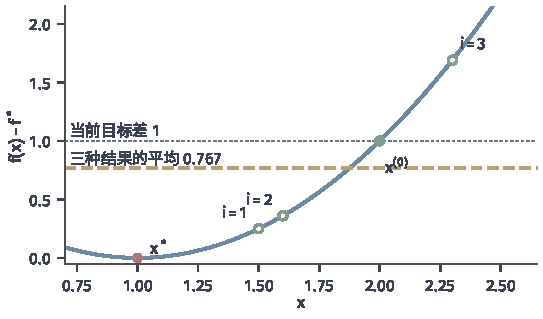
\includegraphics[width=92mm]{figures/05-optimization/05-stochastic-optimization/matplotlib/sgd-single-step/figure.pdf}
  \caption{单步的三种结果。蓝线是目标差$(x-1)^2$，实心绿点是当前点$x^{(0)}=2$，空心绿点是抽到第$i$项后的新点，步长$\alpha=0.1$。第三项使目标差上升到$1.69$，其余两项使它下降。虚线是三种结果的平均$0.767$，低于当前目标差$1$。}
  \label{fig:sgd-single-step}
\end{BookInlineFigure}

式~\eqref{eq:sgd-one-step}给出的数值是相同的。这里$L=2$，$\lvert f'(2)\rvert=2$，条件方差由式~\eqref{eq:sgd-example-variance}是$38/3$，所以下降量和噪声项分别是
\[
 0.1\cdot(1-0.1)\cdot4=0.36,\qquad 0.01\cdot\frac{38}{3}\approx0.127.
\]
于是
\[
 1-0.36+0.127=0.767.
\]
目标是二次函数，下降引理取等号，理论值与实际值完全相同。

\subsection{步长调度}
\label{sec:sgd-step-schedule}

单步分析留下一个问题：步长选大了噪声项大，选小了下降量小，$\alpha^{(t)}$该如何随$t$变化？

\paragraph{固定步长：收敛到一个邻域}
先看步长不变时发生什么。在强凸目标上，初始误差按几何速度消退，噪声则把误差托在一个不为零的水平。

\begin{theorem}[固定步长的误差邻域]
\label{thm:sgd-constant-step}
设$f$的梯度$L$-Lipschitz且$f$是$\mu$强凸的，读数条件无偏，且沿迭代点$\sigma_t^2\leq\sigma^2$。若固定步长$0<\alpha\leq1/L$，则对所有$T\geq0$，
\begin{equation}
 \mathbb{E}[f(\bm{x}^{(T)})]-f^\star\leq(1-\alpha\mu)^T\bigl(f(\bm{x}^{(0)})-f^\star\bigr)+\frac{\alpha L\sigma^2}{2\mu}.
 \label{eq:sgd-constant-step}
\end{equation}
\end{theorem}

\begin{proof}
记$e_t=\mathbb{E}[f(\bm{x}^{(t)})]-f^\star$。因为$\alpha L\leq1$，所以$1-L\alpha/2\geq1/2$，式~\eqref{eq:sgd-one-step}给出
\[
 \mathbb{E}[f(\bm{x}^{(t+1)})\mid\mathcal{F}^{(t)}]\leq f(\bm{x}^{(t)})-\frac{\alpha}{2}\lVert\nabla f(\bm{x}^{(t)})\rVert_2^2+\frac{L\alpha^2}{2}\sigma^2.
\]

强凸性给出对任意$\bm{x},\bm{y}$成立的下界
\[
 f(\bm{y})\geq f(\bm{x})+\langle\nabla f(\bm{x}),\bm{y}-\bm{x}\rangle+\frac{\mu}{2}\lVert\bm{y}-\bm{x}\rVert_2^2.
\]
右端对$\bm{y}$最小化，最小值在$\bm{y}=\bm{x}-\nabla f(\bm{x})/\mu$处取得，所以
\[
 f^\star\geq f(\bm{x})-\frac{1}{2\mu}\lVert\nabla f(\bm{x})\rVert_2^2.
\]
这就是
\[
 \lVert\nabla f(\bm{x})\rVert_2^2\geq2\mu\bigl(f(\bm{x})-f^\star\bigr).
\]

把这个下界代入第一个不等式，两边减去$f^\star$，再取全期望~\eqref{eq:sgd-tower}，得到递推
\[
 e_{t+1}\leq(1-\alpha\mu)e_t+\frac{L\alpha^2\sigma^2}{2}.
\]

由$\alpha\mu\leq\mu/L\leq1$，系数$1-\alpha\mu$非负，递推可以展开$T$次，得到
\[
 e_T\leq(1-\alpha\mu)^Te_0+\frac{L\alpha^2\sigma^2}{2}\sum_{k=0}^{T-1}(1-\alpha\mu)^k.
\]
几何级数不超过$1/(\alpha\mu)$，代入即得式~\eqref{eq:sgd-constant-step}。
\end{proof}

式~\eqref{eq:sgd-constant-step}的第一项随$T$消退，第二项不消退，称为\term{噪声底}（noise floor）。三个条件各有作用：光滑性使下降引理可用，强凸性把梯度大小换算成目标差，方差上界控制每步的损失。去掉强凸性，这个几何递推就不成立；去掉方差上界，噪声项无法用常数控制。

\paragraph{例中的精确递推}
三项目标可以把期望完全算出来。令$\delta_t=x^{(t)}-1$，由$x^{(t+1)}-1=\delta_t-\alpha\hat{g}^{(t)}$和式~\eqref{eq:sgd-example-variance}，条件期望分别是
\[
 \mathbb{E}[\delta_{t+1}\mid\mathcal{F}^{(t)}]=(1-2\alpha)\delta_t,
\]
\[
 \mathbb{E}[\delta_{t+1}^2\mid\mathcal{F}^{(t)}]=\Bigl(1-4\alpha+\frac{14}{3}\alpha^2\Bigr)\delta_t^2-\frac{20}{3}\alpha^2\delta_t+\frac{56}{3}\alpha^2.
\]

当$\alpha<6/7$时，$\delta_t^2$的系数小于$1$，且$\mathbb{E}[\delta_t]\to0$。令$\mathbb{E}[\delta_t^2]$的稳态值为$s$，在第二式中取全期望并令$\mathbb{E}[\delta_t]=0$，它满足
\[
 \Bigl(4\alpha-\frac{14}{3}\alpha^2\Bigr)s=\frac{56}{3}\alpha^2.
\]
解得
\begin{equation}
 \lim_{t\to\infty}\mathbb{E}[f(x^{(t)})-f^\star]=\frac{28\alpha}{6-7\alpha}.
 \label{eq:sgd-example-floor}
\end{equation}
$\alpha=0.1$时噪声底约为$0.528$，$\alpha=0.02$时约为$0.096$。

\begin{BookInlineFigure}
  \centering
  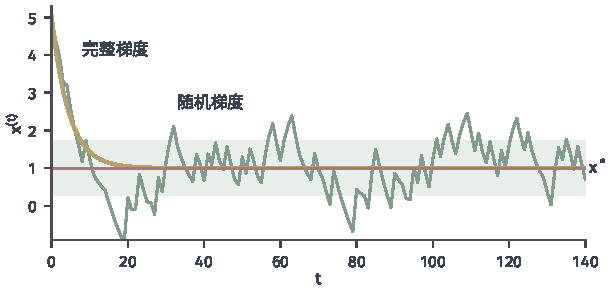
\includegraphics[width=104mm]{figures/05-optimization/05-stochastic-optimization/matplotlib/sgd-sample-path/figure.pdf}
  \caption{三项目标上从$x^{(0)}=5$出发，步长$\alpha=0.1$（种子固定）的一条路径。绿线是随机梯度，黄线是完整梯度，红线是$x^\star=1$。绿底带的半宽是式~\eqref{eq:sgd-example-floor}的平方根$0.727$，即稳态下均方根偏差。}
  \label{fig:sgd-sample-path}
\end{BookInlineFigure}

图~\ref{fig:sgd-sample-path}是一条实际路径。开始的十几步里绿线和黄线几乎重合：离解很远时信号强于噪声，抽到哪一项都往下走。之后黄线停在解上，绿线在一条带内不停抖动，这条带就是噪声底的样子。

\paragraph{固定、递减与分段}
固定步长的两部分误差互相拉扯：大的$\alpha$使初始误差消得快，噪声底却高；小的$\alpha$相反。要想噪声底趋于零，步长就得逐渐减小。

经典的递减条件是
\begin{equation}
 \sum_{t=0}^{\infty}\alpha^{(t)}=\infty,\qquad\sum_{t=0}^{\infty}(\alpha^{(t)})^2<\infty.
 \label{eq:sgd-robbins-monro}
\end{equation}
第一个要求表示累计可走的距离没有上限，初始点再远也到得了；第二个要求表示噪声积累的总量有限\scite{math-robbins1951stochastic}。例如$\alpha^{(t)}=c/(t+t_0)$同时满足两者。

分段调整介于两者之间：先用较大的步长，到达噪声底后减半，再走一段。每段把噪声底压低一半，代价是每段需要的步数翻倍。图~\ref{fig:sgd-step-schedules}(a)比较了几种调度，图中的曲线由递推精确算出。

\begin{BookInlineFigure}
  \centering
  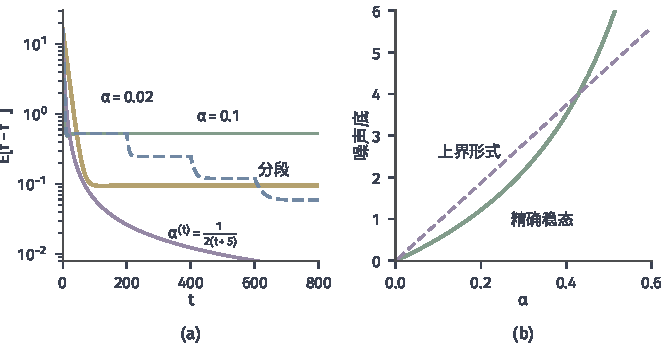
\includegraphics[width=112mm]{figures/05-optimization/05-stochastic-optimization/matplotlib/sgd-step-schedules/figure.pdf}
  \caption{三项目标的步长调度，由精确递推算出，$x^{(0)}=5$。(a)绿线和黄线是固定步长$0.1$和$0.02$，紫线是$\alpha^{(t)}=1/(2(t+5))$，蓝色虚线是从$0.1$起每$200$步减半。固定步长最后变平，大步长到得早而停得高；递减步长持续下降。(b)绿线是噪声底的精确值~\eqref{eq:sgd-example-floor}，紫色虚线是式~\eqref{eq:sgd-constant-step}第二项取$\sigma^2=56/3$的形式；后者只代入最优点处的方差，并非严格上界。步长较大时迭代离解较远，实际方差更大，绿线超过虚线。}
  \label{fig:sgd-step-schedules}
\end{BookInlineFigure}

\paragraph{时间单位}
调度写成$t$的函数时，要说明$t$计的是什么。常见的单位有三种：更新次数、读取的样本量、完整遍历的轮数。批量为$B$、项数为$N$时，一轮是$N/B$次更新，读取$N$个样本。

同一句“每200步减半”，用更新次数计时，批量改变后读取量不同；用样本量计时，批量改变后更新次数不同。批量、并行度或数据量一变，换算不当的调度含义就变了。式~\eqref{eq:sgd-constant-step}和式~\eqref{eq:sgd-robbins-monro}中的$t$都是更新次数。

\paragraph{步长依赖本轮读数时}
前面一直要求$\alpha^{(t)}$在抽样之前确定。步长若依赖本轮读数，$\mathbb{E}[\alpha^{(t)}\hat{\bm{g}}^{(t)}\mid\mathcal{F}^{(t)}]$不再等于$\alpha^{(t)}\nabla f(\bm{x}^{(t)})$，因为步长和方向相关。

在三项目标上看一个具体的后果。取只保留读数符号的规则，步长$\alpha/\lvert\hat{g}\rvert$，每步走固定距离。在$x=0.5$处，三个读数是$3.5,1,-7.5$，真梯度是$-1$，应该向右走。这三个读数的符号是两正一负，平均更新是
\[
 -\alpha\cdot\frac{1+1-1}{3}=-\frac{\alpha}{3},
\]
平均向左走，方向错了。

\begin{BookInlineFigure}
  \centering
  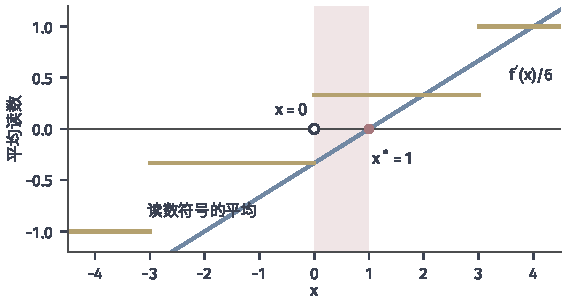
\includegraphics[width=96mm]{figures/05-optimization/05-stochastic-optimization/matplotlib/sgd-normalized-bias/figure.pdf}
  \caption{步长与读数相关时平均方向可能错误。蓝线是真梯度$f'(x)$按比例缩小$6$倍，零点是$x^\star=1$；黄色阶梯是三个读数符号的平均，零点是$x=0$。红底区间$(0,1)$内两者异号，按读数符号走的平均方向与真梯度相反。}
  \label{fig:sgd-normalized-bias}
\end{BookInlineFigure}

图~\ref{fig:sgd-normalized-bias}说明了问题的严重性：这条规则的平均动力学的零点是$x=0$，即各项最小点$-3,0,3$的中位数，而不是$x^\star=1$。缩小$\alpha$也改变不了这一点，因为偏差存在于平均方向之中。依赖读数的步长并非都不能用，后文讨论的方法多属于这一类，但必须分别分析步长与方向的相关性。

\subsection{凸目标的误差与输出}
\label{sec:sgd-convex}

前面的噪声底结论依赖强凸性。对一般的凸目标，$f-f^\star$与梯度大小没有固定的换算关系，下降引理的路线走不通。这一小节换一个量来追踪：到最优解的距离。

\paragraph{距离递推与平均点}
距离的好处是展开之后能用凸性。把更新代入$\lVert\bm{x}^{(t+1)}-\bm{x}^\star\rVert_2^2$，内积项由凸性转成目标差，所得到的结论是对迭代点的加权和成立的。

为了从加权和回到一个点，需要Jensen不等式：若$f$凸，$\lambda_t\geq0$，$\sum_t\lambda_t=1$，则
\[
 f\Bigl(\sum_t\lambda_t\bm{x}^{(t)}\Bigr)\leq\sum_t\lambda_tf(\bm{x}^{(t)}).
\]
两个点的情形就是凸函数的定义，多个点时对点数作归纳即得。

\begin{theorem}[凸目标的加权平均点]
\label{thm:sgd-convex}
设$f$凸且可微，存在最小点$\bm{x}^\star$，读数条件无偏，且沿迭代点读数的条件二阶矩不超过$G^2$，步长$\alpha^{(t)}>0$事先确定。记$R=\lVert\bm{x}^{(0)}-\bm{x}^\star\rVert_2$，$A_T=\sum_{t=0}^{T-1}\alpha^{(t)}$，加权平均点
\begin{equation}
 \bar{\bm{x}}^{(T)}=\frac{1}{A_T}\sum_{t=0}^{T-1}\alpha^{(t)}\bm{x}^{(t)}.
 \label{eq:sgd-weighted-average}
\end{equation}
则
\begin{equation}
 \mathbb{E}[f(\bar{\bm{x}}^{(T)})]-f^\star\leq\frac{R^2+G^2\sum_{t=0}^{T-1}(\alpha^{(t)})^2}{2A_T}.
 \label{eq:sgd-convex-bound}
\end{equation}
\end{theorem}

\begin{proof}
记$d_t$为$\lVert\bm{x}^{(t)}-\bm{x}^\star\rVert_2^2$的期望。展开平方，得到
\[
 \lVert\bm{x}^{(t+1)}-\bm{x}^\star\rVert_2^2=\lVert\bm{x}^{(t)}-\bm{x}^\star\rVert_2^2-2\alpha^{(t)}\langle\hat{\bm{g}}^{(t)},\bm{x}^{(t)}-\bm{x}^\star\rangle+(\alpha^{(t)})^2\lVert\hat{\bm{g}}^{(t)}\rVert_2^2.
\]

取$\mathbb{E}[\cdot\mid\mathcal{F}^{(t)}]$。$\bm{x}^{(t)}-\bm{x}^\star$由历史确定，内积项由条件无偏变成$\langle\nabla f(\bm{x}^{(t)}),\bm{x}^{(t)}-\bm{x}^\star\rangle$。凸性给出
\[
 \langle\nabla f(\bm{x}^{(t)}),\bm{x}^{(t)}-\bm{x}^\star\rangle\geq f(\bm{x}^{(t)})-f^\star.
\]

再用二阶矩的上界并取全期望，得到递推
\[
 d_{t+1}\leq d_t-2\alpha^{(t)}\bigl(\mathbb{E}[f(\bm{x}^{(t)})]-f^\star\bigr)+(\alpha^{(t)})^2G^2.
\]

对$t=0,\ldots,T-1$求和，左右的$d_t$逐项相消，再丢掉非负的$d_T$，得到
\[
 2\sum_{t=0}^{T-1}\alpha^{(t)}\bigl(\mathbb{E}[f(\bm{x}^{(t)})]-f^\star\bigr)\leq R^2+G^2\sum_{t=0}^{T-1}(\alpha^{(t)})^2.
\]

两边除以$2A_T$，并对$\lambda_t=\alpha^{(t)}/A_T$使用Jensen不等式，即得式~\eqref{eq:sgd-convex-bound}。
\end{proof}

固定步长$\alpha$时，式~\eqref{eq:sgd-convex-bound}的右端是$R^2/(2\alpha T)+\alpha G^2/2$。对$\alpha$求最小，取$\alpha=R/(G\sqrt{T})$，得到
\begin{equation}
 \mathbb{E}[f(\bar{\bm{x}}^{(T)})]-f^\star\leq\frac{RG}{\sqrt{T}}.
 \label{eq:sgd-convex-rate}
\end{equation}
要把目标差减小十倍，步数要增加一百倍。

二阶矩的上界$G^2$包含了梯度本身，在全空间常常不成立。若$f$还有$L$-Lipschitz梯度，条件可以放宽为条件方差不超过$\sigma^2$。在凸的$L$-光滑函数上，从$\bm{x}$走一步$\bm{x}-\nabla f(\bm{x})/L$，由下降引理，
\[
 f^\star\leq f(\bm{x})-\frac{1}{2L}\lVert\nabla f(\bm{x})\rVert_2^2.
\]
于是梯度大小被目标差控制，读数的二阶矩满足
\[
 \mathbb{E}[\lVert\hat{\bm{g}}^{(t)}\rVert_2^2\mid\mathcal{F}^{(t)}]\leq2L\bigl(f(\bm{x}^{(t)})-f^\star\bigr)+\sigma^2.
\]

把它代入上面的递推，当$\alpha\leq1/(2L)$时，由$1-\alpha L\geq1/2$，同样的求和给出
\begin{equation}
 \mathbb{E}[f(\bar{\bm{x}}^{(T)})]-f^\star\leq\frac{R^2}{\alpha T}+\alpha\sigma^2.
 \label{eq:sgd-convex-smooth}
\end{equation}
取$\alpha=\min\{1/(2L),R/(\sigma\sqrt{T})\}$，右端不超过$2LR^2/T+2R\sigma/\sqrt{T}$。第一项是完整梯度下降的速率，第二项是噪声带来的代价；$\sigma=0$时退回确定情形。

\paragraph{强凸性的改善}
强凸性使距离递推有了收缩，步长可以取到$1/t$的量级。

\begin{theorem}[强凸目标的递减步长]
\label{thm:sgd-strong-decay}
设$f$可微且$\mu$强凸，读数条件无偏，沿迭代点读数的条件二阶矩不超过$G^2$，$\alpha^{(t)}=1/(\mu(t+1))$。则对所有$T\geq1$，
\begin{equation}
 \mathbb{E}[\lVert\bm{x}^{(T)}-\bm{x}^\star\rVert_2^2]\leq\frac{G^2}{\mu^2T}.
 \label{eq:sgd-strong-rate}
\end{equation}
\end{theorem}

\begin{proof}
强凸下界中分别取$(\bm{x},\bm{x}^\star)$和$(\bm{x}^\star,\bm{x})$，相加并用$\nabla f(\bm{x}^\star)=\bm{0}$，得到
\[
 \langle\nabla f(\bm{x}),\bm{x}-\bm{x}^\star\rangle\geq\mu\lVert\bm{x}-\bm{x}^\star\rVert_2^2.
\]
沿用定理~\ref{thm:sgd-convex}证明中的展开，得到
\[
 d_{t+1}\leq(1-2\alpha^{(t)}\mu)d_t+(\alpha^{(t)})^2G^2=\Bigl(1-\frac{2}{t+1}\Bigr)d_t+\frac{G^2}{\mu^2(t+1)^2}.
\]

对$T$作归纳。$T=1$时，取$t=0$，系数是$-1$，由$d_0\geq0$有$d_1\leq G^2/\mu^2$，结论成立。

设$d_t\leq G^2/(\mu^2t)$，其中$t\geq1$，此时系数$1-2/(t+1)$非负。代入递推，得到
\[
 d_{t+1}\leq\frac{G^2}{\mu^2}\Bigl[\frac{t-1}{t(t+1)}+\frac{1}{(t+1)^2}\Bigr].
\]

只需证明方括号不超过$1/(t+1)$，即$\tfrac{t-1}{t}+\tfrac{1}{t+1}\leq1$。这等价于$\tfrac{1}{t+1}\leq\tfrac{1}{t}$，成立。
\end{proof}

强凸假设和全空间的$G^2$是矛盾的，因为强凸函数的梯度无界。定理中的条件要理解为迭代点在有界集内，通常由投影到有界闭凸集来保证，投影不增大到$\bm{x}^\star$的距离，上面的递推继续成立。

把结论总结成对比：

\begin{BookInlineTable}
  \centering
  \begin{tabular}{lll}
    \toprule
    条件 & 步长 & 期望误差\\
    \midrule
    凸，二阶矩有界 & $\dfrac{R}{G\sqrt{T}}$ & 平均点目标差$\dfrac{RG}{\sqrt{T}}$\\\addlinespace[2.5mm]
    凸，光滑，方差有界 & $\min\Bigl\{\dfrac{1}{2L},\dfrac{R}{\sigma\sqrt{T}}\Bigr\}$ & 平均点目标差$\dfrac{2LR^2}{T}+\dfrac{2R\sigma}{\sqrt{T}}$\\\addlinespace[2.5mm]
    强凸，二阶矩有界 & $\dfrac{1}{\mu(t+1)}$ & 末点距离平方$\dfrac{G^2}{\mu^2T}$\\\addlinespace[2.5mm]
    强凸，光滑，方差有界 & 固定，$\alpha\leq\dfrac1L$ & 末点目标差，含噪声底\\
    \bottomrule
  \end{tabular}
  \caption{本小节及上一小节的保证。表中“末点”指最后一个迭代点，“光滑”指梯度$L$-Lipschitz。前两行的结论针对平均点，后两行针对末点。}
  \label{tab:sgd-rates}
\end{BookInlineTable}

\paragraph{最后一点与平均点}
定理~\ref{thm:sgd-convex}的保证属于平均点，不能搬到任意一个迭代点上。平均值小只说明大多数项小：序列$0,0,\ldots,0,3$的平均可以任意小，而最后一项是$3$。一般凸目标上最后一点的保证需要单独证明，所得的速率通常比平均点差，具体分析较长，读者可查阅专门的文献。

\begin{BookInlineFigure}
  \centering
  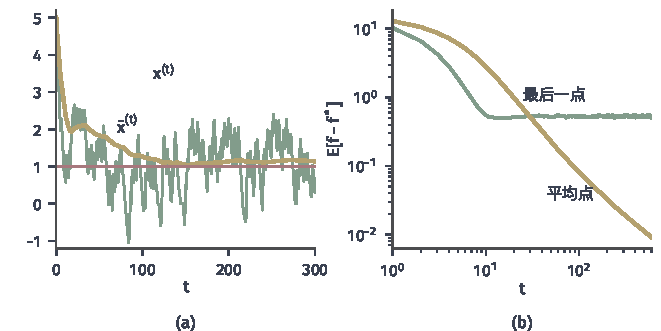
\includegraphics[width=112mm]{figures/05-optimization/05-stochastic-optimization/matplotlib/sgd-average-vs-last/figure.pdf}
  \caption{三项目标上固定步长$\alpha=0.1$，从$x^{(0)}=5$出发。(a)同一条路径上最后一点$x^{(t)}$（绿）和从头算起的平均点$\bar{x}^{(t)}$（黄），红线是$x^\star$。(b)$4000$次独立运行的平均目标差（种子固定），两轴取对数。$t=600$时最后一点的目标差约为$0.53$，平均点约为$0.009$。}
  \label{fig:sgd-average-vs-last}
\end{BookInlineFigure}

在三项目标上平均的作用很明显。图~\ref{fig:sgd-average-vs-last}(a)的绿线一直在抖，黄线很快贴近解。(b)说明最后一点停在噪声底$0.53$，平均点的目标差继续下降。原因是抖动在解的两侧来回，平均时相互抵消，而初始段的影响被越来越多的项稀释。平均点要付出的代价是多存一个向量，并且受早期迭代点的拖累，因此实践中也常只平均后面一段。

\subsection{非凸目标的误差与输出}
\label{sec:sgd-nonconvex}

目标非凸时，到最小点的距离既不能保证下降，也可能不止一个最小点。只能回到单步下降，评价的量也要换成梯度大小。

\paragraph{累加下降量}
式~\eqref{eq:sgd-one-step}不需要凸性，把它沿$t$累加，左边望远镜相消，剩下函数值的总下降量，它受目标下界限制。

\begin{theorem}[非凸目标的平均平方梯度]
\label{thm:sgd-nonconvex}
设$f$有下界$f_{\inf}$，梯度$L$-Lipschitz，读数条件无偏且沿迭代点$\sigma_t^2\leq\sigma^2$，步长事先确定且$0<\alpha^{(t)}\leq1/L$。记$\Delta=f(\bm{x}^{(0)})-f_{\inf}$，$A_T=\sum_{t=0}^{T-1}\alpha^{(t)}$。则
\begin{equation}
 \frac{1}{A_T}\sum_{t=0}^{T-1}\alpha^{(t)}\mathbb{E}[\lVert\nabla f(\bm{x}^{(t)})\rVert_2^2]\leq\frac{2\Delta+L\sigma^2\sum_{t=0}^{T-1}(\alpha^{(t)})^2}{A_T}.
 \label{eq:sgd-nonconvex-bound}
\end{equation}
\end{theorem}

\begin{proof}
由$\alpha^{(t)}L\leq1$，式~\eqref{eq:sgd-one-step}的系数$1-L\alpha^{(t)}/2\geq1/2$。取全期望，得到
\[
 \frac{\alpha^{(t)}}{2}\mathbb{E}[\lVert\nabla f(\bm{x}^{(t)})\rVert_2^2]\leq\mathbb{E}[f(\bm{x}^{(t)})]-\mathbb{E}[f(\bm{x}^{(t+1)})]+\frac{L(\alpha^{(t)})^2}{2}\sigma^2.
\]

对$t=0,\ldots,T-1$求和，函数值逐项相消，只剩$f(\bm{x}^{(0)})-\mathbb{E}[f(\bm{x}^{(T)})]$，由下界，它不超过$\Delta$。于是
\[
 \frac12\sum_{t=0}^{T-1}\alpha^{(t)}\mathbb{E}[\lVert\nabla f(\bm{x}^{(t)})\rVert_2^2]\leq\Delta+\frac{L\sigma^2}{2}\sum_{t=0}^{T-1}(\alpha^{(t)})^2.
\]
两边乘以$2/A_T$，即得式~\eqref{eq:sgd-nonconvex-bound}。
\end{proof}

固定步长时，右端是$2\Delta/(\alpha T)+L\sigma^2\alpha$。取
\[
 \alpha=\min\Bigl\{\frac1L,\ \sqrt{\frac{2\Delta}{L\sigma^2T}}\Bigr\},
\]
并利用$1/\alpha$不超过两个倒数之和，得到
\begin{equation}
 \frac{1}{T}\sum_{t=0}^{T-1}\mathbb{E}[\lVert\nabla f(\bm{x}^{(t)})\rVert_2^2]\leq\frac{2L\Delta}{T}+2\sqrt{\frac{2L\Delta\sigma^2}{T}}.
 \label{eq:sgd-nonconvex-rate}
\end{equation}

\paragraph{按权重随机返回}
式~\eqref{eq:sgd-nonconvex-bound}的左端是平均，还不是某个点的性质。非凸时平均点没有Jensen不等式可用，点的平均甚至可能落在山顶上。解决办法是把平均变成一个随机的点：以概率$\alpha^{(t)}/A_T$抽取下标$\tau$，返回$\bm{x}^{(\tau)}$。由全期望公式，
\[
 \mathbb{E}[\lVert\nabla f(\bm{x}^{(\tau)})\rVert_2^2]=\frac{1}{A_T}\sum_{t=0}^{T-1}\alpha^{(t)}\mathbb{E}[\lVert\nabla f(\bm{x}^{(t)})\rVert_2^2].
\]
所以左端是这个随机输出的期望平方梯度。

用一个能实际计算的非凸例子来看。取$f_i(x)=1-\cos x+c_ix$，$(c_1,c_2,c_3)=(-2,0,2)$，则
\[
 f(x)=1-\cos x,\qquad f_i'(x)=\sin x+c_i.
\]
这里$f_{\inf}=0$，$L=1$，条件方差恰好是常数$\sigma^2=8/3$，所有假设都严格成立。取$x^{(0)}=2.5$，$\alpha=0.1$，$T=800$，则$\Delta=1-\cos2.5\approx1.80$，上界是
\[
 \frac{2\cdot1.80}{0.1\cdot800}+1\cdot\frac83\cdot0.1\approx0.045+0.267=0.312.
\]

\begin{BookInlineFigure}
  \centering
  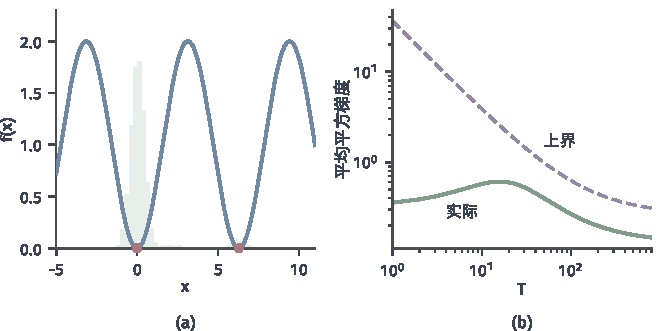
\includegraphics[width=112mm]{figures/05-optimization/05-stochastic-optimization/matplotlib/sgd-nonconvex-output/figure.pdf}
  \caption{非凸目标$f(x)=1-\cos x$上$6000$次独立运行的随机梯度方法（种子固定），$x^{(0)}=2.5$，$\alpha=0.1$。(a)蓝线是目标函数，红点是最小点$x=0$和$2\pi$，绿底直方图是$T=800$时按权重随机返回的点的分布（纵向已缩放）。(b)绿线是$T$步内平方梯度的平均，紫色虚线是式~\eqref{eq:sgd-nonconvex-bound}的上界，两轴取对数。}
  \label{fig:sgd-nonconvex-output}
\end{BookInlineFigure}

图~\ref{fig:sgd-nonconvex-output}(b)显示实际平均约为$0.147$，低于上界$0.312$。上界的第二项$\alpha L\sigma^2$对应的正是噪声底，这个上界在$T$增大时不趋于零，要趋于零必须同时缩小$\alpha$。图(a)中大多数返回点集中在$x=0$附近，少数越过山峰到了$2\pi$附近。

\paragraph{这个结论不说明什么}
式~\eqref{eq:sgd-nonconvex-bound}只评价一阶驻定。小梯度的点可能在鞍点或平坦的高处，它与局部极小的距离没有被保证；能否离开鞍点是第~\ref{chap:saddle-points}章的主题。

它也是期望界，不是逐路径保证。由Markov不等式，对$\varepsilon>0$，
\[
 \mathbb{P}\bigl(\lVert\nabla f(\bm{x}^{(\tau)})\rVert_2^2\geq\varepsilon\bigr)\leq\frac{\mathbb{E}[\lVert\nabla f(\bm{x}^{(\tau)})\rVert_2^2]}{\varepsilon},
\]
只给出一次运行的概率控制。随着$t\to\infty$路径本身的行为，例如几乎处处收敛，需要鞅收敛等工具，可参考\BookChapterRef{chap:discrete-time-stochastic-processes}{卷九第3章“离散时间随机过程”}。

\subsection{随机邻近梯度}
\label{sec:sgd-proximal}

目标带非光滑项时，上面的更新不能直接用。本小节要解决的问题是：非光滑项确定而光滑项需要抽样，邻近步该怎样接上随机读数？

\paragraph{主要思想}
设复合目标$F(\bm{x})=f(\bm{x})+h(\bm{x})$，其中$f$是光滑的有限和或期望目标，$h$是适当、下半连续的凸函数，且邻近映射可以计算。\term{随机邻近梯度法}（stochastic proximal gradient method）只对光滑部分抽样，$h$则每步精确处理：
\begin{equation}
 \bm{x}^{(t+1)}=\operatorname{prox}_{\alpha^{(t)}h}\bigl(\bm{x}^{(t)}-\alpha^{(t)}\hat{\bm{g}}^{(t)}\bigr),
 \label{eq:sgd-prox-update}
\end{equation}
其中邻近映射的定义和计算见第~\ref{chap:nonsmooth-composite-optimization}章。$h$不参与抽样，只在邻近步中出现，这样$\hat{\bm{g}}^{(t)}$的条件无偏性只关系到$f$。

\paragraph{计算过程}
在三项目标上加$h(x)=\gamma\lvert x\rvert$，取$\gamma=1$。复合目标的最优解满足$2x-2+\gamma=0$，所以$x^\star=0.5$，它是正的，与$\lvert x\rvert$的导数取$+1$相符。邻近映射是软阈值：
\[
 \operatorname{prox}_{\alpha h}(z)=\operatorname{sign}(z)\max\{\lvert z\rvert-\alpha\gamma,0\}.
\]
变量与第~\ref{sec:sgd-basic}小节相同，多一个非光滑项的参数。每轮更新三步：抽样下标$i^{(t)}$，走一步随机梯度得到中间点$\bm{z}^{(t)}$，求$\bm{z}^{(t)}$的邻近点作为$\bm{x}^{(t+1)}$。

例中取$x^{(t)}=0.2$，$\alpha=0.1$，阈值是$0.1$。三项读数分别是$3.2,0.4,-8.4$，完整梯度是$-1.6$。走完梯度步的三种结果是
\[
 z=-0.12,\quad z=0.16,\quad z=1.04,
\]
对应的邻近点分别是
\[
 -0.02,\quad 0.06,\quad 0.94.
\]

\paragraph{随机更新的均值不等于精确更新}
三个邻近点的平均是$0.327$。精确更新则先平均梯度，$z=0.36$，邻近点是$0.26$。两者不相等。

\begin{BookInlineFigure}
  \centering
  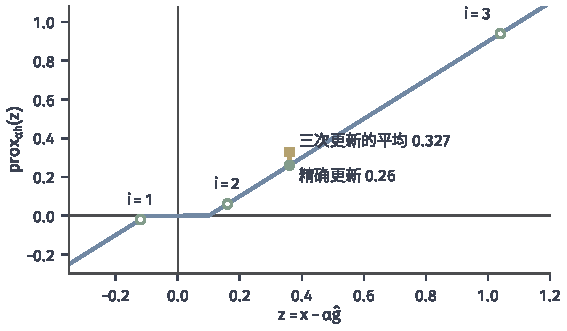
\includegraphics[width=96mm]{figures/05-optimization/05-stochastic-optimization/matplotlib/sgd-prox-bias/figure.pdf}
  \caption{邻近映射的非线性。蓝线是阈值为$0.1$的软阈值函数。三个空心点是三种读数对应的结果。实心绿点是先平均$z$再求邻近点的精确更新，黄方块是三次邻近点的平均。两点之差来自软阈值在零附近的弯折。}
  \label{fig:sgd-prox-bias}
\end{BookInlineFigure}

图~\ref{fig:sgd-prox-bias}说明了原因：邻近映射是非线性的，先平均再映射与先映射再平均结果不同。所以即使$\hat{\bm{g}}^{(t)}$条件无偏，随机更新的均值一般也不等于精确更新。这就是不能直接沿用无偏分析的地方。

\paragraph{误差的评价}
凸情形用复合目标差评价。证明的关键是引入精确更新点，把含噪声的内积拆开。

\begin{theorem}[随机邻近梯度的平均点]
\label{thm:sgd-prox}
设$f$凸且梯度$L$-Lipschitz，$h$适当、下半连续、凸，$F=f+h$有最小点$\bm{x}^\star$。读数条件无偏，沿迭代点$\sigma_t^2\leq\sigma^2$，固定步长$0<\alpha\leq1/L$。记$R=\lVert\bm{x}^{(0)}-\bm{x}^\star\rVert_2$，$\bar{\bm{x}}^{(T)}$为$\bm{x}^{(1)},\ldots,\bm{x}^{(T)}$的算术平均，则
\begin{equation}
 \mathbb{E}[F(\bar{\bm{x}}^{(T)})]-F(\bm{x}^\star)\leq\frac{R^2}{2\alpha T}+\alpha\sigma^2.
 \label{eq:sgd-prox-bound}
\end{equation}
\end{theorem}

\begin{proof}
证明中把当前点和下一点记为$\bm{x},\bm{x}^+$，噪声记为$\bm{\zeta}$，比较点$\bm{u}$取为$\bm{x}^\star$。由下降引理和$f$的凸性，
\[
 f(\bm{x}^+)\leq f(\bm{u})+\langle\nabla f(\bm{x}),\bm{x}^+-\bm{u}\rangle+\frac{L}{2}\lVert\bm{x}^+-\bm{x}\rVert_2^2.
\]

邻近点的最优性条件说明$(\bm{x}-\alpha\hat{\bm{g}}^{(t)}-\bm{x}^+)/\alpha$是$h$在$\bm{x}^+$处的次梯度，于是
\[
 h(\bm{x}^+)\leq h(\bm{u})-\langle\hat{\bm{g}}^{(t)},\bm{x}^+-\bm{u}\rangle+\frac{1}{\alpha}\langle\bm{x}-\bm{x}^+,\bm{x}^+-\bm{u}\rangle.
\]

把两式相加。对最后的内积使用恒等式
\[
 2\langle\bm{x}-\bm{x}^+,\bm{x}^+-\bm{u}\rangle=\lVert\bm{x}-\bm{u}\rVert_2^2-\lVert\bm{x}^+-\bm{u}\rVert_2^2-\lVert\bm{x}^+-\bm{x}\rVert_2^2.
\]
由$\alpha\leq1/L$，$\lVert\bm{x}^+-\bm{x}\rVert_2^2$的系数$L/2-1/(2\alpha)$非正，可以丢掉，得到
\[
 F(\bm{x}^+)-F(\bm{u})\leq\frac{\lVert\bm{x}-\bm{u}\rVert_2^2-\lVert\bm{x}^+-\bm{u}\rVert_2^2}{2\alpha}-\langle\bm{\zeta},\bm{x}^+-\bm{u}\rangle.
\]

最后一项里$\bm{x}^+$依赖$\bm{\zeta}$，条件期望不为零。这里引入用真梯度算出的精确更新点
\[
 \bm{p}=\operatorname{prox}_{\alpha h}\bigl(\bm{x}-\alpha\nabla f(\bm{x})\bigr).
\]
它由历史确定，于是
\[
 \mathbb{E}[\langle\bm{\zeta},\bm{p}-\bm{u}\rangle\mid\mathcal{F}^{(t)}]=0.
\]

邻近映射是非扩张的，两个输入相差$\alpha\bm{\zeta}$，所以$\bm{x}^+$与$\bm{p}$的距离不超过$\alpha\lVert\bm{\zeta}\rVert_2$。再由Cauchy--Schwarz不等式，
\[
 -\langle\bm{\zeta},\bm{x}^+-\bm{p}\rangle\leq\alpha\lVert\bm{\zeta}\rVert_2^2.
\]

取条件期望，得到
\[
 \mathbb{E}[F(\bm{x}^+)\mid\mathcal{F}^{(t)}]-F(\bm{u})\leq\frac{\lVert\bm{x}-\bm{u}\rVert_2^2-\mathbb{E}[\lVert\bm{x}^+-\bm{u}\rVert_2^2\mid\mathcal{F}^{(t)}]}{2\alpha}+\alpha\sigma^2.
\]
取全期望后对$t=0,\ldots,T-1$求和，距离项逐项相消，再除以$T$，并由$F$的凸性用Jensen不等式，即得式~\eqref{eq:sgd-prox-bound}。
\end{proof}

非凸的光滑部分要用另一种度量。精确邻近梯度映射是
\begin{equation}
 \bm{G}_\alpha(\bm{x})=\frac{1}{\alpha}\Bigl[\bm{x}-\operatorname{prox}_{\alpha h}\bigl(\bm{x}-\alpha\nabla f(\bm{x})\bigr)\Bigr],
 \label{eq:sgd-prox-mapping}
\end{equation}
$\bm{G}_\alpha(\bm{x})=\bm{0}$恰好是复合目标的驻点条件。把$\nabla f$换成读数就得到含噪声的读数，它不能代替驻点残差。例中$x=0.2$处$G_\alpha=(0.2-0.26)/0.1=-0.6$，而三次含噪读数是$2.2$，$1.4$，$-7.4$，平均$-1.27$，既不等于$-0.6$，也没有哪一次接近它。这种读数变小，不能说明当前点接近驻点。

\subsection{随机块更新}
\label{sec:sgd-block}

第~\ref{chap:block-optimization}章的分块方法每步只更新变量的一块。本节的方法每步只读一部分目标项。两者可以同时使用，这时要说清每种随机选择各带来什么。

\paragraph{两种随机选择}
把变量分成$J$块，第$j$块的偏梯度记为$\nabla_jf$，$\bm{U}_j$把第$j$块的向量放回全长向量的相应位置，其余分量补零。随机块更新在第$t$步选一块$j^{(t)}$，抽一项$i^{(t)}$，然后
\begin{equation}
 \bm{x}^{(t+1)}=\bm{x}^{(t)}-\alpha_{j^{(t)}}\bm{U}_{j^{(t)}}\nabla_{j^{(t)}}f_{i^{(t)}}(\bm{x}^{(t)}).
 \label{eq:sgd-block-update}
\end{equation}
选块是对变量抽样，选项是对目标项抽样，图~\ref{fig:sgd-block-item-grid}用一张二维表表示。

\begin{BookInlineFigure}
  \centering
  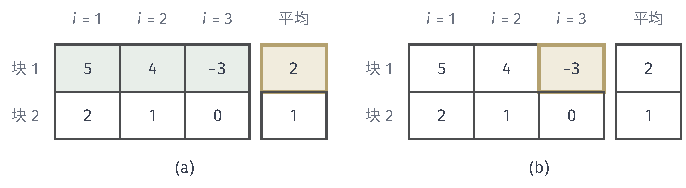
\includegraphics[width=112mm]{figures/05-optimization/05-stochastic-optimization/tikz/sgd-block-item-grid/figure.pdf}
  \caption{读取一次的范围。行是变量块，列是目标项，表中数字是第$i$项对第$j$块的偏导。(a)只随机选块：读完一行所有项（绿底），得到精确的偏梯度（黄框）。(b)同时选块和选项：只读一格（黄框），这个数是偏导的一次读数。}
  \label{fig:sgd-block-item-grid}
\end{BookInlineFigure}

用二元的例子把数字写出来。把贯穿例的$x$记作$x_1$，再加一个变量$x_2$，令第$i$项是
\[
 f_i(x_1,x_2)=\frac{a_i}{2}(x_1-b_i)^2+\frac12(x_2-c_i)^2,\qquad(c_1,c_2,c_3)=(-1,0,1).
\]
在$(2,1)$处，第一块的三个偏导是$5,4,-3$，平均$2$；第二块的三个偏导是$2,1,0$，平均$1$。

\paragraph{固定历史后的核对}
分两层取条件期望。先固定历史和选中的块$j$，只对目标项求平均，由式~\eqref{eq:sgd-uniform-mean}得到
\[
 \mathbb{E}\bigl[\nabla_jf_{i^{(t)}}(\bm{x}^{(t)})\mid\mathcal{F}^{(t)},j\bigr]=\nabla_jf(\bm{x}^{(t)}).
\]
所以给定块之后读数对这一块的偏梯度无偏，条件方差记为$\sigma_j^2$。这一条要求选项的抽样分布不依赖于这一步的读数。若先把各块的读数算出来，再选读数最大的块，结果就有偏。

对选中的块使用块光滑常数$L_j$，第~\ref{chap:block-optimization}章的块下降引理给出的单步界与式~\eqref{eq:sgd-one-step}同样推导：
\begin{equation}
 \begin{aligned}
 \mathbb{E}[f(\bm{x}^{(t+1)})\mid\mathcal{F}^{(t)},j]
 \leq{}&f(\bm{x}^{(t)})-\alpha_j\Bigl(1-\frac{L_j\alpha_j}{2}\Bigr)\lVert\nabla_jf(\bm{x}^{(t)})\rVert_2^2\\
 &+\frac{L_j\alpha_j^2}{2}\sigma_j^2.
 \end{aligned}
 \label{eq:sgd-block-one-step}
\end{equation}

\paragraph{两类随机性并存时}
再对块的选择求平均。取块均匀，$\alpha_j=1/L_j$，由式~\eqref{eq:sgd-block-one-step}，
\[
 \mathbb{E}[f(\bm{x}^{(t+1)})\mid\mathcal{F}^{(t)}]\leq f(\bm{x}^{(t)})-\frac{1}{J}\sum_{j=1}^{J}\frac{\lVert\nabla_jf(\bm{x}^{(t)})\rVert_2^2}{2L_j}+\frac{1}{J}\sum_{j=1}^{J}\frac{\sigma_j^2}{2L_j}.
\]
只随机选块时$\sigma_j=0$，退回第~\ref{chap:block-optimization}章的结论，读取一行的成本是$N$项对这一块的偏导。同时抽样时，一次更新只读一格，代价小得多，但多出噪声项，邻域和步长都要像上面那样处理。

步长也要按两种随机性分别考虑：块步长$\alpha_j$由块光滑常数决定，抽样噪声则要求更小的步长或方差控制。一个容易犯的错误是把噪声项算成所有块的方差之和，而每次其实只读一块；另一个错误是只对选项取期望，忘记选块也是随机的。例中在$(2,1)$处，选块均匀、$\alpha_j=0.1$时，平均更新量是
\[
 -\frac12\cdot0.1\cdot(2,1)=(-0.1,-0.05).
\]
这是两层平均的结果：选中第一块时第一个分量的平均更新是$-0.2$，第二个分量不变，第二块反过来。一次实际抽样中，比如选第一块、第三项，更新量是$(+0.3,0)$，这与平均方向相反，与第~\ref{sec:sgd-unbiased}小节的单项读数相反的情形相同。

\section{方差控制}
\label{sec:sgd-variance}

上一节的误差界都有一项与噪声方差$\sigma^2$成正比。目标和精度要求固定时，把这一项压下去就能用更少的更新达到相同的结果。有哪些办法减小读数的方差，每种办法又要付出多少读取、存储和维护成本？这两件事必须一起看，方差减小不等于总计算减少。

三类办法依次是：一次多读几项，改变抽项的分布，利用已经读过的梯度。

\subsection{小批量与梯度累积}
\label{sec:sgd-minibatch}

\paragraph{批量平均的方差}
最直接的办法是一次读$B$项取平均。设给定历史后$\hat{\bm{g}}_1,\ldots,\hat{\bm{g}}_B$独立同分布，且都是$\nabla f(\bm{x})$的无偏读数，条件方差为$\sigma^2$。\term{小批量}（mini-batch）读数是
\begin{equation}
 \hat{\bm{g}}_{(B)}=\frac{1}{B}\sum_{k=1}^{B}\hat{\bm{g}}_k.
 \label{eq:sgd-minibatch}
\end{equation}

记$\bm{\zeta}_k=\hat{\bm{g}}_k-\nabla f(\bm{x})$。把平方展开，分成平方项和交叉项：
\[
 \mathbb{E}\Bigl[\Bigl\lVert\frac{1}{B}\sum_{k}\bm{\zeta}_k\Bigr\rVert_2^2\;\Big|\;\mathcal{F}^{(t)}\Bigr]
 =\frac{1}{B^2}\sum_{k}\mathbb{E}[\lVert\bm{\zeta}_k\rVert_2^2\mid\mathcal{F}^{(t)}]+\frac{1}{B^2}\sum_{k\neq l}\mathbb{E}[\langle\bm{\zeta}_k,\bm{\zeta}_l\rangle\mid\mathcal{F}^{(t)}].
\]

给定历史时$\bm{\zeta}_k$和$\bm{\zeta}_l$独立且条件均值为零，所以内积的条件期望等于两个条件均值的内积，即零。平方项一共$B$个，所以
\begin{equation}
 \operatorname{Var}\bigl[\hat{\bm{g}}_{(B)}\mid\mathcal{F}^{(t)}\bigr]=\frac{\sigma^2}{B}.
 \label{eq:sgd-minibatch-variance}
\end{equation}
关键在于交叉项消失，这是独立带来的。若读数之间相关，交叉项不再为零，须把它们的协方差保留在展开式中。

\paragraph{无放回的方差}
从$N$项中无放回地抽$B$项，读数不独立，交叉项有确定的值。记$\bm{v}_i=\nabla f_i(\bm{x})-\nabla f(\bm{x})$，它们的和是零，平均平方是$\sigma^2$。对$\lVert\sum_i\bm{v}_i\rVert_2^2=0$展开，得到
\[
 \sum_{i}\lVert\bm{v}_i\rVert_2^2+\sum_{i\neq j}\langle\bm{v}_i,\bm{v}_j\rangle=0.
\]
所以不同的两项的内积平均是$-\sigma^2/(N-1)$。

把这个值代入上面的展开式，交叉项一共$B(B-1)$个，得到
\begin{equation}
 \operatorname{Var}\bigl[\hat{\bm{g}}_{(B)}\mid\mathcal{F}^{(t)}\bigr]=\frac{\sigma^2}{B}\cdot\frac{N-B}{N-1}.
 \label{eq:sgd-minibatch-no-replacement}
\end{equation}
因子$(N-B)/(N-1)$小于$1$。$B=N$时方差为零，正是读完全部的情形。

在三项目标的$x^\star$处核对，这时$\sigma^2=56/3$，读数$(4,2,-6)$的和是零。取$B=2$无放回，三种配对的平均读数是$3,\,-1,\,-2$，平方的平均是
\[
 \frac{9+1+4}{3}=\frac{14}{3}.
\]
公式~\eqref{eq:sgd-minibatch-no-replacement}给出同一结果：$\tfrac{56/3}{2}\cdot\tfrac12=\tfrac{14}{3}$。有放回的$B=2$则是$28/3$，多了一倍。

\begin{BookInlineFigure}
  \centering
  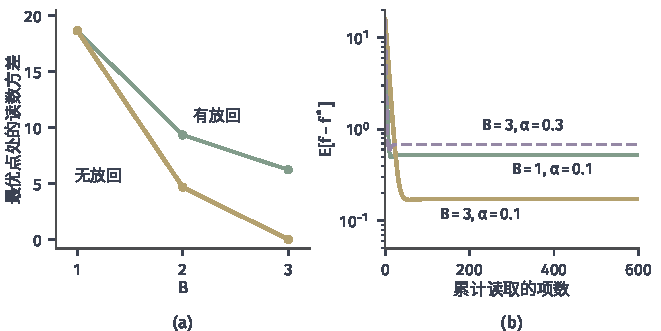
\includegraphics[width=112mm]{figures/05-optimization/05-stochastic-optimization/matplotlib/sgd-minibatch-variance/figure.pdf}
  \caption{小批量的方差与成本，三项目标。(a)最优点处读数方差随批量的变化，绿线有放回，黄线无放回，$B=3$时无放回的方差为零。(b)从$x^{(0)}=5$出发的期望目标差，由精确递推算出，横轴是累计读取的项数。绿线$B=1$，黄线$B=3$且步长相同，紫色虚线$B=3$且步长乘以$3$。}
  \label{fig:sgd-minibatch-variance}
\end{BookInlineFigure}

\paragraph{方差减小不等于计算减少}
式~\eqref{eq:sgd-minibatch-variance}让噪声项除以$B$，但读取量乘以$B$。图~\ref{fig:sgd-minibatch-variance}(b)说明了两者的权衡。步长不变时，$B=3$的噪声底从$0.53$降到$0.17$；把步长也放大$3$倍，保持每次读取走过的距离不变，$B=3$的噪声底是$0.68$，并不比$B=1$更好，初始阶段的下降也差不多。在步长可以随批量调整的范围内，增加批量和缩小步长的效果大体相同，总读取量并没有节省。

增加批量的价值在别处：多个读数可以并行计算，矩阵运算可以成批进行，方差小了也允许使用更稳健的步长。这些是实现上的收益，须按实际硬件单独计算。

\paragraph{梯度累积}
批量太大、一次放不进内存时，可以把它拆成若干微批量，分别算梯度后加起来，只更新一次，这称为\term{梯度累积}（gradient accumulation）。设批量$B$拆成微批量，大小为$n_1,\ldots,n_K$，$\sum_kn_k=B$。设第$k$个微批量的平均读数为$\hat{\bm{g}}_k$，累积时必须按样本数加权：
\begin{equation}
 \hat{\bm{g}}_{(B)}=\sum_{k=1}^{K}\frac{n_k}{B}\hat{\bm{g}}_k.
 \label{eq:sgd-accumulation}
\end{equation}

\begin{BookInlineFigure}
  \centering
  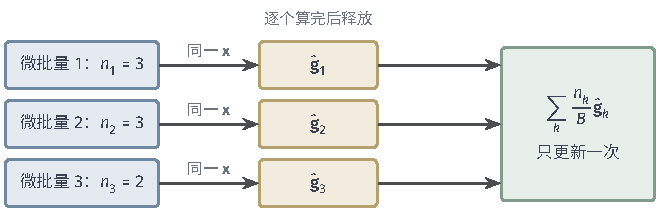
\includegraphics[width=112mm]{figures/05-optimization/05-stochastic-optimization/tikz/sgd-gradient-accumulation/figure.pdf}
  \caption{梯度累积。批量$8$拆成大小为$3,3,2$的微批量。参数在整个过程中保持不变，每个微批量的梯度算完就可以释放它占用的样本与中间结果。累积时按$n_k/B$加权，全部读完后才更新一次。}
  \label{fig:sgd-gradient-accumulation}
\end{BookInlineFigure}

图~\ref{fig:sgd-gradient-accumulation}显示了三个要求。第一，整个累积过程中参数$\bm{x}$不变，否则各微批量的梯度算在不同的点上，加起来不是一个点的梯度。第二，目标函数不变，包括确定的正则项只加一次。第三，权重按样本数计。三项目标上把第一、二项作为一个微批量，第三项单独作为一个，$x=2$处
\[
 \frac23\cdot\frac{5+4}{2}+\frac13\cdot(-3)=2,
\]
与三项的平均相同。若不加权，直接平均两个微批量的读数，得到$(4.5-3)/2=0.75$，答案错了。

读数若还依赖批内统计量，例如用批内均值做归一化，拆开后微批量的统计量与整批不同，累积结果不再等于整批的结果，这些统计量要在整批范围内统一更新。

梯度累积减少的只是同时占用的存储，总读取量仍是$B$。它不是一种降低方差的新办法，只是用更长的时间换更少的内存，方差与整批相同。

\subsection{非均匀抽样}
\label{sec:sgd-importance}

有些项的梯度大，有些小。均匀抽样对所有项一视同仁，把更多机会给“重要”的项，能否减小方差？

\paragraph{逆概率权重}
以固定的正概率$p_1,\ldots,p_N$抽项，$\sum_ip_i=1$。为使条件均值仍是完整梯度，要给读数加上逆概率权重：
\begin{equation}
 \hat{\bm{g}}=\frac{1}{Np_i}\nabla f_i(\bm{x})+\nabla r(\bm{x}).
 \label{eq:sgd-importance-estimator}
\end{equation}
确定的正则梯度$\nabla r$无需抽样，单独加入。条件均值按概率加权直接计算，分母上的$p_i$与概率相消：
\[
 \sum_{i=1}^{N}p_i\cdot\frac{1}{Np_i}\nabla f_i(\bm{x})+\nabla r(\bm{x})=\frac{1}{N}\sum_{i=1}^{N}\nabla f_i(\bm{x})+\nabla r(\bm{x}).
\]
这就是式~\eqref{eq:sgd-finite-sum-regularized}的完整梯度。这种做法称为\term{非均匀抽样}（non-uniform sampling），权重也称重要性权重。

权重不能省略。第~\ref{sec:sgd-unbiased}小节的概率$(1/2,1/4,1/4)$在不加权时，实际被最小化的是加权目标$\tfrac12f_1+\tfrac14f_2+\tfrac14f_3$，它的梯度是
\[
 \frac12(x+3)+\frac14\cdot2x+\frac14(3x-9)=\frac74x-\frac34.
\]
零点是$x=3/7$，而不是$x^\star=1$。算法的不动点取决于读数的条件均值，而不取决于更新的形式。

\paragraph{不同概率下的二阶矩}
无偏之后比较方差，只需比较二阶矩，因为均值已固定。设$r=0$，读数$\tfrac{1}{Np_i}\nabla f_i$的二阶矩是
\begin{equation}
 M(\bm{p})=\sum_{i=1}^{N}p_i\Bigl\lVert\frac{\nabla f_i(\bm{x})}{Np_i}\Bigr\rVert_2^2=\frac{1}{N^2}\sum_{i=1}^{N}\frac{\lVert\nabla f_i(\bm{x})\rVert_2^2}{p_i}.
 \label{eq:sgd-importance-second-moment}
\end{equation}

由Cauchy--Schwarz不等式，
\[
 \Bigl(\sum_i\lVert\nabla f_i\rVert_2\Bigr)^2\leq\Bigl(\sum_i\frac{\lVert\nabla f_i\rVert_2^2}{p_i}\Bigr)\Bigl(\sum_ip_i\Bigr).
\]
于是$M(\bm{p})$的最小值是$(\sum_i\lVert\nabla f_i\rVert_2)^2/N^2$，在$p_i\propto\lVert\nabla f_i(\bm{x})\rVert_2$时取到。最优概率依赖当前点，而算出它需要读完全部的项，这与抽样的目的相矛盾。

在三项目标的$x^\star$处，读数是$(4,2,-6)$，代入式~\eqref{eq:sgd-importance-second-moment}比较三种概率：
\[
 \begin{aligned}
 \bm{p}=\bigl(\tfrac13,\tfrac13,\tfrac13\bigr):\quad&M=\tfrac{56}{3}\approx18.67,\\
 \bm{p}\propto(L_1,L_2,L_3)=\bigl(\tfrac16,\tfrac13,\tfrac12\bigr):\quad&M=20,\\
 \bm{p}\propto(\lvert4\rvert,\lvert2\rvert,\lvert{-6}\rvert)=\bigl(\tfrac13,\tfrac16,\tfrac12\bigr):\quad&M=16.
 \end{aligned}
\]
常用的$p_i\propto L_i$在这个点上比均匀更差。这种选择有另外的好处：加权后各项的光滑常数$L_i/(Np_i)$相同，都等于$\bar{L}=\tfrac1N\sum_iL_i=2$，而不再是$L_{\max}=3$。依赖逐项光滑常数的步长上界因此放宽。

\begin{BookInlineFigure}
  \centering
  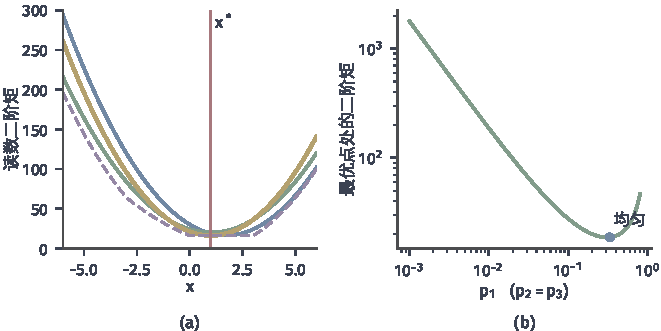
\includegraphics[width=112mm]{figures/05-optimization/05-stochastic-optimization/matplotlib/sgd-importance-sampling/figure.pdf}
  \caption{非均匀抽样的二阶矩，三项目标。(a)不同固定概率下的读数二阶矩随$x$的变化：蓝线均匀，绿线$p_i\propto L_i$，黄线$p_i\propto\lvert f_i'(x^\star)\rvert$，紫色虚线是每点都用最优概率的下包络，红线是$x^\star$。(b)最优点处二阶矩随$p_1$的变化，$p_2=p_3=(1-p_1)/2$，两轴取对数，蓝点是均匀抽样。}
  \label{fig:sgd-importance-sampling}
\end{BookInlineFigure}

图~\ref{fig:sgd-importance-sampling}(a)显示，三条曲线在不同位置各有胜负。没有哪个固定的分布处处最好，这是最优概率依赖$\bm{x}$的直接表现。图(b)说明另一个危险：概率过小会放大读数。$p_1=0.01$时第一项读数被放大$1/(3\cdot0.01)\approx33$倍，$x^\star$处的二阶矩升到约$187$，是均匀抽样的十倍。一项只要可能有非零梯度，就要给它不太小的概率。

代价方面要算三笔账。计算概率需要各项的$L_i$或梯度范数的估计；维护离散分布、每次抽样需要合适的数据结构，概率更新后还要维护；若各项尺度相近，这些投入得不到回报。只有各项差异明显、概率容易得到时，非均匀抽样才值得使用。

\subsection{SVRG}
\label{sec:sgd-svrg}

小批量靠多读减小方差，方差只能按$1/B$下降，到最优点也不消失。有没有办法让读数的方差随迭代点靠近解而自动趋于零？图~\ref{fig:sgd-term-gradients}(b)的观察给出了线索：三条单项导数虽然不同，但都是光滑变化的，在相邻两点的差别不大。

\paragraph{主要思想}
控制变量的想法是：如果要估计一个数，手里还有一个与它高度相关且均值已知的量，就可以用它来纠偏。这里的已知量是一个旧点的梯度。

选一个快照点$\tilde{\bm{x}}$，事先计算好它的完整梯度$\nabla f(\tilde{\bm{x}})$。此后每一步抽$i$，用同一项在当前点和快照点的梯度差，加上快照的完整梯度：
\begin{equation}
 \hat{\bm{g}}=\nabla f_i(\bm{x})-\nabla f_i(\tilde{\bm{x}})+\nabla f(\tilde{\bm{x}}).
 \label{eq:sgd-svrg-direction}
\end{equation}
这就是\term{SVRG}（stochastic variance reduced gradient）\scite{johnson2013accelerating}的方向。$\nabla f_i(\tilde{\bm{x}})$称为\term{控制变量}（control variate）。

对$i$求条件平均，第一项是$\nabla f(\bm{x})$，后两项相消：
\[
 \mathbb{E}[\hat{\bm{g}}\mid\mathcal{F}^{(t)}]=\nabla f(\bm{x})-\nabla f(\tilde{\bm{x}})+\nabla f(\tilde{\bm{x}})=\nabla f(\bm{x}).
\]
所以$\hat{\bm{g}}$条件无偏，这里不需要任何关于$\tilde{\bm{x}}$的假设。方差却取决于$\bm{x}$和$\tilde{\bm{x}}$的距离：若$\bm{x}=\tilde{\bm{x}}$，$\hat{\bm{g}}$恰为完整梯度，一点噪声也没有。

三项目标的读数是一次函数，修正后的方向很简单：
\[
 \hat{g}=a_i(x-\tilde{x})+f'(\tilde{x}).
\]

\begin{BookInlineFigure}
  \centering
  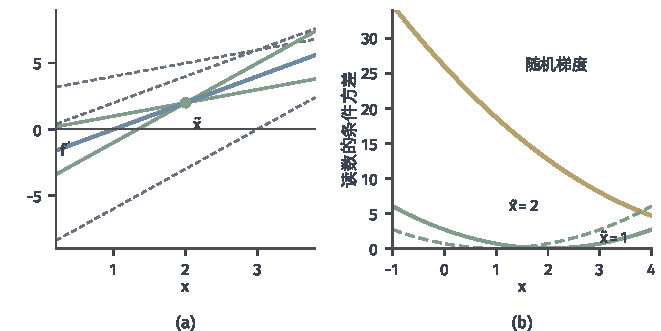
\includegraphics[width=112mm]{figures/05-optimization/05-stochastic-optimization/matplotlib/sgd-svrg-fan/figure.pdf}
  \caption{SVRG的纠偏，三项目标，快照$\tilde{x}=2$。(a)虚线是原始的三项读数，绿线是修正后的读数，蓝线是$f'$。修正后的三条线都经过快照处的点$(2,f'(2))$。(b)读数的条件方差随$x$的变化：黄线是普通随机梯度，绿实线是快照$\tilde{x}=2$，绿虚线是快照$\tilde{x}=1=x^\star$。}
  \label{fig:sgd-svrg-fan}
\end{BookInlineFigure}

图~\ref{fig:sgd-svrg-fan}(a)说明了修正的几何含义：原始的三条读数线各自散开，修正后都绕着快照处的完整梯度旋转，$x$越接近快照，分散越小。条件方差的表达式是$\tfrac23(x-\tilde{x})^2$，它在$x=\tilde{x}$处为零，这正是图(b)的绿线。比较$x=1$这一点，快照$\tilde{x}=2$时条件方差是$2/3$，普通随机梯度是$56/3$。

快照要不断更新。随着$\bm{x}$收敛，把快照移过来，图(b)的绿线就从实线变成虚线，方差在解处变成零。这样，算法每隔若干步要花一次完整梯度的成本重新设置快照，因此有内外两层循环，如图~\ref{fig:sgd-svrg-loop}所示。

\begin{BookInlineFigure}
  \centering
  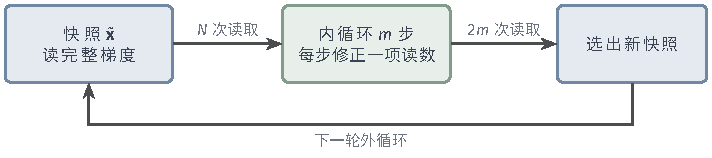
\includegraphics[width=110mm]{figures/05-optimization/05-stochastic-optimization/tikz/sgd-svrg-loop/figure.pdf}
  \caption{SVRG的两层循环。外循环计算完整梯度（$N$次读取）并存下快照，内循环运行$m$步，每步用式~\eqref{eq:sgd-svrg-direction}，读取同一项在两点的梯度（$2$次读取）。一轮外循环共$N+2m$次读取。}
  \label{fig:sgd-svrg-loop}
\end{BookInlineFigure}

\needspace{6\baselineskip}
\paragraph{变量}
\begin{itemize}
 \item $\tilde{\bm{x}}\in\mathbb{R}^n$：快照点。
 \item $\tilde{\bm{g}}\in\mathbb{R}^n$：快照点的完整梯度$\nabla f(\tilde{\bm{x}})$。
 \item $\bm{x}^{(t)}\in\mathbb{R}^n$：内循环的当前点，$t=0,\ldots,m$。
 \item $\alpha>0$，$m$：步长和内循环长度。
\end{itemize}

\paragraph{初始化}
取初始快照$\tilde{\bm{x}}$。例中取$\tilde{x}=2$，$\alpha=0.05$，这满足后面定理的条件，由式~\eqref{eq:sgd-example-gradients}，
\[
 \tilde{g}=f'(2)=2.
\]

\paragraph{每轮更新}
外循环的一轮按下列步骤进行。

\begin{enumerate}
 \item 快照：置$\bm{x}^{(0)}=\tilde{\bm{x}}$，计算$\tilde{\bm{g}}=\nabla f(\tilde{\bm{x}})$，共$N$次读取。例中$x^{(0)}=2$，$\tilde{g}=2$。
 \item 内循环：对$t=0,\ldots,m-1$，抽下标$i^{(t)}$，按式~\eqref{eq:sgd-svrg-direction}得到方向$\hat{\bm{g}}^{(t)}$，沿它走步长$\alpha$得到新点。

 例中第一步抽到$i=3$，$x^{(0)}=\tilde{x}$，方向就是完整梯度，
 \[
  \hat{g}^{(0)}=2,\qquad x^{(1)}=2-0.05\cdot2=1.9.
 \]

 第二步抽到$i=1$，$a_1=1$，方向和新点是
 \[
  \hat{g}^{(1)}=1\cdot(1.9-2)+2=1.9,\qquad x^{(2)}=1.9-0.05\cdot1.9=1.805.
 \]

 第三步抽到$i=2$，$a_2=2$，方向和新点是
 \[
  \hat{g}^{(2)}=2\cdot(1.805-2)+2=1.61,\qquad x^{(3)}=1.805-0.05\cdot1.61=1.7245.
 \]
 \item 选取新快照：从内循环的点中选一个作为新的$\tilde{\bm{x}}$。下面的定理要求在$\bm{x}^{(0)},\ldots,\bm{x}^{(m-1)}$中均匀随机选取，实践中也常取最后一点。
\end{enumerate}

外循环达到预定轮数后结束。最终得到最后一次的快照。例中三步都朝$x^\star=1$靠近，方向全部为正，没有再出现单项读数$-3$带来的上坡，这正是控制变量的效果。

\paragraph{差分的方差与收敛}
证明方差自动减小的关键，是用目标差控制逐项梯度的差。需要假设每一项都是光滑的凸函数。

\begin{lemma}[逐项梯度差的控制]
\label{lem:sgd-gradient-difference}
设$f_i$凸且梯度$L$-Lipschitz，$f=\frac1N\sum_if_i$有最小点$\bm{x}^\star$。则对任意$\bm{x}$，
\begin{equation}
 \frac{1}{N}\sum_{i=1}^{N}\lVert\nabla f_i(\bm{x})-\nabla f_i(\bm{x}^\star)\rVert_2^2\leq2L\bigl(f(\bm{x})-f^\star\bigr).
 \label{eq:sgd-gradient-difference}
\end{equation}
\end{lemma}

\begin{proof}
定义
\[
 \psi_i(\bm{x})=f_i(\bm{x})-f_i(\bm{x}^\star)-\langle\nabla f_i(\bm{x}^\star),\bm{x}-\bm{x}^\star\rangle.
\]
$\psi_i$凸，梯度$L$-Lipschitz，$\nabla\psi_i(\bm{x}^\star)=\bm{0}$，所以$\bm{x}^\star$是它的最小点，最小值为$0$。

对$\psi_i$从$\bm{x}$走一步$\bm{x}-\nabla\psi_i(\bm{x})/L$，由下降引理，
\[
 0\leq\psi_i\Bigl(\bm{x}-\frac{1}{L}\nabla\psi_i(\bm{x})\Bigr)\leq\psi_i(\bm{x})-\frac{1}{2L}\lVert\nabla\psi_i(\bm{x})\rVert_2^2.
\]

$\nabla\psi_i(\bm{x})$就是$\nabla f_i(\bm{x})$与$\nabla f_i(\bm{x}^\star)$的差。对$i$平均时，由$\nabla f(\bm{x}^\star)=\bm{0}$，一次项消失，$\psi_i$的平均恰为$f(\bm{x})-f^\star$。整理即得式~\eqref{eq:sgd-gradient-difference}。
\end{proof}

\begin{theorem}[SVRG的线性收缩]
\label{thm:sgd-svrg}
设每个$f_i$凸且梯度$L$-Lipschitz，$f$是$\mu$强凸的。设$0<\alpha<1/(4L)$，$m$足够大，使
\begin{equation}
 \rho=\frac{1}{\mu\alpha(1-2L\alpha)m}+\frac{2L\alpha}{1-2L\alpha}<1.
 \label{eq:sgd-svrg-rate}
\end{equation}
每轮外循环的新快照在$\bm{x}^{(0)},\ldots,\bm{x}^{(m-1)}$中均匀随机选取。则相邻两轮的快照$\tilde{\bm{x}}_{s}$，$\tilde{\bm{x}}_{s+1}$满足
\begin{equation}
 \mathbb{E}[f(\tilde{\bm{x}}_{s+1})]-f^\star\leq\rho\bigl(\mathbb{E}[f(\tilde{\bm{x}}_s)]-f^\star\bigr).
 \label{eq:sgd-svrg-contraction}
\end{equation}
\end{theorem}

\begin{proof}
固定一轮外循环，$\tilde{\bm{x}}$由此前的历史确定。记$\bm{x}=\bm{x}^{(t)}$，$E_x=f(\bm{x})-f^\star$，$E_s=f(\tilde{\bm{x}})-f^\star$。先控制方向的二阶矩。

在方向~\eqref{eq:sgd-svrg-direction}中加减$\nabla f_i(\bm{x}^\star)$，把它写成两段之和，再用不等式$(a+b)^2\leq2a^2+2b^2$，得到
\[
 \lVert\hat{\bm{g}}\rVert_2^2\leq2\lVert\nabla f_i(\bm{x})-\nabla f_i(\bm{x}^\star)\rVert_2^2+2\lVert\nabla f_i(\tilde{\bm{x}})-\nabla f_i(\bm{x}^\star)-\nabla f(\tilde{\bm{x}})\rVert_2^2.
\]

第二段里，$\nabla f_i(\tilde{\bm{x}})-\nabla f_i(\bm{x}^\star)$的条件均值恰为$\nabla f(\tilde{\bm{x}})$，第二段就是它减去自己的均值。方差不超过二阶矩，所以去掉$\nabla f(\tilde{\bm{x}})$后条件期望不会变小。对两段分别用式~\eqref{eq:sgd-gradient-difference}，得到
\[
 \mathbb{E}[\lVert\hat{\bm{g}}\rVert_2^2\mid\mathcal{F}^{(t)}]\leq4L(E_x+E_s).
\]

再展开距离。由条件无偏和$f$的凸性，内积项不小于$E_x$，于是
\[
 \mathbb{E}[\lVert\bm{x}^{(t+1)}-\bm{x}^\star\rVert_2^2\mid\mathcal{F}^{(t)}]\leq\lVert\bm{x}-\bm{x}^\star\rVert_2^2-2\alpha E_x+4L\alpha^2(E_x+E_s).
\]

对$t=0,\ldots,m-1$求和取全期望，距离项相消，并丢掉非负的终点距离。记$\bar{E}$为内循环点目标差的平均，它也是随机选出的新快照的期望目标差，得到
\[
 2\alpha(1-2L\alpha)m\bar{E}\leq\mathbb{E}\lVert\tilde{\bm{x}}-\bm{x}^\star\rVert_2^2+4L\alpha^2m\mathbb{E}[E_s].
\]

强凸性给出快照点的距离上界$\tfrac{2}{\mu}E_s$，代入后得到
\[
 2\alpha(1-2L\alpha)m\bar{E}\leq\Bigl(\frac{2}{\mu}+4L\alpha^2m\Bigr)\mathbb{E}[E_s].
\]
两边除以$2\alpha(1-2L\alpha)m$，即得式~\eqref{eq:sgd-svrg-contraction}。
\end{proof}

式~\eqref{eq:sgd-svrg-rate}的两项分别表示：内循环够长，初始距离的影响才能被摊薄；步长够小，快照带来的方差项才小于收缩。这里$L$是单项的光滑常数，在三项目标上$L=3$，$\mu=2$。取$\alpha=0.05<1/12$，$m=50$，得到
\[
 \rho=\frac{1}{2\cdot0.05\cdot0.7\cdot50}+\frac{0.3}{0.7}\approx0.286+0.429=0.714.
\]
这是一个保守的上界。三项目标从$\tilde{x}=2$开始一轮的实际结果，用$20000$次独立运行的平均来估计，目标差约从$1$降到$0.115$。

\paragraph{成本}
一轮外循环需要$N+2m$次读取，每轮把目标差减小一个固定比例。取$\alpha$为$1/L$的小常数倍、$m$与$\kappa$同量级时$\rho$是小于$1$的常数，所以减小一个固定比例约需$N+\kappa$量级的读取，这里$\kappa=L/\mu$用单项的光滑常数计算。完整梯度下降减小同样的比例约需$N\kappa_f$量级的读取，其中$\kappa_f$用$f$本身的光滑常数计算。$N$很大时前者优势明显。存储上，SVRG只保存$\tilde{\bm{x}}$和$\tilde{\bm{g}}$两个向量，每步重新计算$\nabla f_i(\tilde{\bm{x}})$。也可以事先保存所有项的快照梯度，每步只需一次读取，但内存要多$N$个向量。内循环长度$m$、快照的频率，在理论和实践之间常有差别，定理的$m$往往偏大。

SVRG要求能重复访问所有项，且每轮要算一次完整梯度，所以只适用于有限和目标；样本源源不断的期望目标不能直接用。

\subsection{SAGA}
\label{sec:sgd-saga}

SVRG要定期花一次完整梯度来设置快照。如果把每一项上次读到的梯度都记下来，是不是不用专门做快照，靠记忆逐步更新就够了？这就是SAGA\scite{defazio2014saga}的想法。

\paragraph{主要思想}
为每一项维护一个存下的旧梯度$\bm{\phi}_i$，以及它们的均值$\bar{\bm{\phi}}=\frac1N\sum_i\bm{\phi}_i$。每一步抽$i$，用新读数减去这一项的旧读数，再加上旧均值：
\begin{equation}
 \hat{\bm{g}}=\nabla f_i(\bm{x})-\bm{\phi}_i+\bar{\bm{\phi}}.
 \label{eq:sgd-saga-direction}
\end{equation}
这与SVRG的方向形式相同，只是把快照点的梯度换成了各项自己记录的旧梯度。给定历史，表项都是确定的，对$i$求条件平均，第二、三项相消，所以方向条件无偏。

完成参数更新之后，才把表项$\bm{\phi}_i$替换成新读数，并同步修改均值：
\begin{equation}
 \bar{\bm{\phi}}\leftarrow\bar{\bm{\phi}}+\frac{1}{N}\bigl(\nabla f_i(\bm{x})-\bm{\phi}_i\bigr).
 \label{eq:sgd-saga-mean}
\end{equation}
这个次序不能交换。若先把$\bm{\phi}_i$换成新读数，方向就变成$\bar{\bm{\phi}}$，只是旧梯度的平均，新读数根本没有进入更新，条件无偏也失去了。

\needspace{6\baselineskip}
\paragraph{变量}
\begin{itemize}
 \item $\bm{x}^{(t)}\in\mathbb{R}^n$：当前点。
 \item $\bm{\phi}_i\in\mathbb{R}^n$，$i=1,\ldots,N$：各项记录的旧梯度，共$N$个向量。
 \item $\bar{\bm{\phi}}\in\mathbb{R}^n$：表项的均值，用式~\eqref{eq:sgd-saga-mean}增量更新，不必每次重算。
 \item $\alpha>0$：步长。
\end{itemize}

\paragraph{初始化}
在初始点读全部$N$项填满梯度表，$N$次读取。例中取$x^{(0)}=2$，$\alpha=0.05$，表项和均值是
\[
 (\phi_1,\phi_2,\phi_3)=(5,4,-3),\qquad \bar{\phi}=2.
\]

\paragraph{每轮更新}
对$t=0,1,\ldots$依次执行以下步骤。

\begin{enumerate}
 \item 抽样并读取：抽$i^{(t)}$，计算新读数$\nabla f_{i^{(t)}}(\bm{x}^{(t)})$，这是一次读取。例中第一轮抽到$i=3$，新读数是$-3$。
 \item 计算方向并更新：由式~\eqref{eq:sgd-saga-direction}，例中第一轮
 \[
  \hat{g}^{(0)}=-3-(-3)+2=2,\qquad x^{(1)}=2-0.05\cdot2=1.9.
 \]
 \item 更新表项：把$\bm{\phi}_{i^{(t)}}$换成新读数，按式~\eqref{eq:sgd-saga-mean}修改均值。例中第一轮新读数与旧表项相同，$\phi_3$和均值都不变。
\end{enumerate}

例中第二轮抽到$i=1$，新读数$f_1'(1.9)=4.9$，方向和新点是
\[
 \hat{g}^{(1)}=4.9-5+2=1.9,\qquad x^{(2)}=1.9-0.05\cdot1.9=1.805.
\]
然后$\phi_1$变成$4.9$，均值变成$(4.9+4-3)/3\approx1.967$。

例中第三轮抽到$i=2$，新读数$f_2'(1.805)=3.61$，方向和新点是
\[
 \hat{g}^{(2)}\approx3.61-4+1.967=1.577,\qquad x^{(3)}\approx1.805-0.05\cdot1.577=1.726.
\]
然后$\phi_2$变成$3.61$，均值变成$(4.9+3.61-3)/3\approx1.837$。图~\ref{fig:sgd-saga-table}画出了表的变化。

\begin{BookInlineFigure}
  \centering
  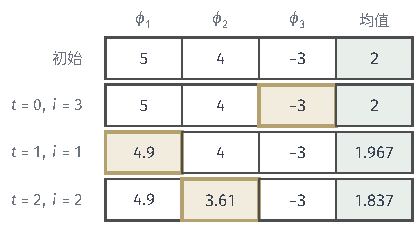
\includegraphics[width=72mm]{figures/05-optimization/05-stochastic-optimization/tikz/sgd-saga-table/figure.pdf}
  \caption{SAGA的梯度表在三步内的变化。每行是完成该步之后的表，黄框是刚被替换的项，右列是表的均值。第一步新读数恰好等于旧表项，表不变；此后只有被抽到的项发生变化。}
  \label{fig:sgd-saga-table}
\end{BookInlineFigure}

迭代在读取量达到预定预算后结束，最终得到$\bm{x}^{(T)}$；例中三步后$x^{(3)}\approx1.726$，每步一次读取，加上初始化的三次，共六次读取。

\paragraph{两种误差共同评价}
SAGA的状态比普通方法多一张表，所以进展要同时看两件事：参数离解多远，表项离各自的$\nabla f_i(\bm{x}^\star)$多远。参数接近解之后，表项还可能很旧，方差还不会小。要让方差趋于零，就需要每一项都被更新到解附近。

\begin{theorem}[SAGA的线性收敛]
\label{thm:sgd-saga}
设每个$f_i$凸且梯度$L$-Lipschitz，$f$是$\mu$强凸的，取$\alpha=1/(3L)$，下标独立均匀抽取，梯度表在初始点填满。则存在只依赖初始距离和初始表项误差的常数$C$，使
\begin{equation}
 \mathbb{E}[\lVert\bm{x}^{(T)}-\bm{x}^\star\rVert_2^2]\leq\Bigl(1-\min\Bigl\{\frac{1}{4N},\frac{\mu}{3L}\Bigr\}\Bigr)^TC.
 \label{eq:sgd-saga-rate}
\end{equation}
\end{theorem}

式~\eqref{eq:sgd-saga-rate}的证明需要构造一个同时包含距离和各表项误差的函数，并证明它的期望按上述比例收缩，推导较长，读者可查阅原始论文\scite{defazio2014saga}。这里解释结论的机制。速率的最小值中有两项：$\mu/(3L)$与单纯的梯度下降类似，由条件数决定；$1/(4N)$反映表项的刷新速度，每一步只刷新一项，刷新一遍大约需要$N$步。$N$很大时，记忆更新是瓶颈，反过来则是条件数决定收敛。

在三项目标上，$N=3$，$L=3$，$\mu=2$，所以
\[
 \min\Bigl\{\frac{1}{12},\frac29\Bigr\}=\frac{1}{12},
\]
定理保证的是每步收缩$11/12$。手算所用的$\alpha=0.05$小于$1/(3L)=1/9$，只用来演示表项的变化。

SAGA没有强凸性时也有保证，平均点的目标差按$1/T$的量级下降，常数与$N$有关，这里不再讨论。

\paragraph{比较}
表~\ref{tab:sgd-vr-compare}按读取和存储比较这些方法。方差控制的共同代价是：多读或多存，并依赖逐项光滑、凸性等结构。

\begin{BookInlineTable}
  \centering
  \begin{tabular}{llll}
    \toprule
    方法 & 每次更新读取 & 存储 & 需要重复访问\\
    \midrule
    随机梯度 & $1$ & $1$个向量 & 否\\
    小批量 & $B$ & $1$个向量 & 否\\
    SVRG & $2$，另有每轮$N$ & $2$个向量 & 是\\
    SAGA & $1$，初始化$N$ & $N+2$个向量 & 是\\
    \bottomrule
  \end{tabular}
  \caption{方差控制方法的成本。存储只计迭代所需向量，随机梯度和小批量含当前点。}
  \label{tab:sgd-vr-compare}
\end{BookInlineTable}

SAGA的表要存$N$个$n$维向量，这在$N$和$n$都很大时是沉重的负担。对各项梯度是某个数乘已知向量的线性模型，每个表项只需存一个标量，才算切实可行。

图~\ref{fig:sgd-vr-cost}用一个$N=500$、$n=20$的正则最小二乘实例比较总读取量。横轴是读取量除以$N$，即完整遍历的轮数。随机梯度初期最快，但很快到达噪声底。完整梯度稳定下降，但每步代价是$N$。SVRG和SAGA在初期略慢于随机梯度，此后保持线性收敛，目标差继续下降到比噪声底小许多个量级的水平。

\begin{BookInlineFigure}
  \centering
  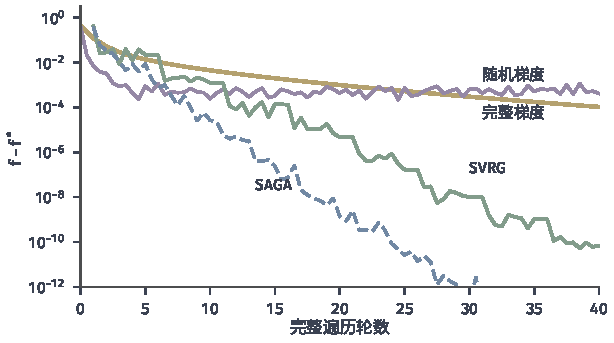
\includegraphics[width=104mm]{figures/05-optimization/05-stochastic-optimization/matplotlib/sgd-vr-cost/figure.pdf}
  \caption{总读取量与目标差，$N=500$、$n=20$的正则最小二乘实例（种子固定），$\lVert\bm{a}_i\rVert_2=1$，$\gamma=0.005$。黄线是完整梯度，紫线是固定步长$0.1$的随机梯度，绿线是SVRG（$\alpha=0.2/L$，$m=2N$，此处$L$取单项的光滑常数），蓝色虚线是SAGA（$\alpha=1/(3L)$）。横轴是读取量除以$N$，纵轴取对数。}
  \label{fig:sgd-vr-cost}
\end{BookInlineFigure}

这个比较的结论有边界：只针对这一个实例和这一组参数，SVRG和SAGA的优势在需要高精度时才明显。若只需低精度，或者问题本身的噪声底已经够用，普通随机梯度加小批量更简单；若数据是流式的，不能重复访问，这两种方法都用不上。

\section{随机动量方法}
\label{sec:sgdb-momentum}

小批量和控制变量都在改善单步的读数，代价是多读梯度或多存梯度。本节换一个问题：不增加读取，只把已经读过的梯度组合进当前方向，能得到什么，又要付出什么？

组合历史读数有两种效果。一致的成分累积起来，随机涨落互相抵消，这是平滑；旧读数来自旧的位置，当前梯度变化时方向跟不上，这是滞后。两者同时发生，而且历史进入了算法的状态，每一步的误差要连同历史一起分析。本节先讲当前点读数的重球法，再讲前瞻点读数的Nesterov方法，最后讲两种把动量做非线性变换的方法。

\subsection{随机重球法}
\label{sec:sgdb-heavy-ball}

\paragraph{主要思想}
第~\ref{chap:first-order-methods}章的重球法在当前梯度步之外，再加上一步历史位移。把其中的梯度换成当前点的随机读数$\hat{\bm g}^{(t)}$，就得到\term{随机重球法}（stochastic heavy ball method）。规定$\bm{x}^{(-1)}=\bm{x}^{(0)}$，
\begin{equation}
 \bm{x}^{(t+1)}=\bm{x}^{(t)}-\alpha\hat{\bm g}^{(t)}+\beta\bigl(\bm{x}^{(t)}-\bm{x}^{(t-1)}\bigr),\qquad 0\leq\beta<1.
 \label{eq:sgdb-hb}
\end{equation}

式~\eqref{eq:sgdb-hb}要存两个位置。实际计算常改写成只存一个速度向量$\bm{v}^{(t)}$的形式：取$\bm{v}^{(0)}=\bm{0}$，先更新速度，再更新位置，
\begin{equation}
 \bm{v}^{(t+1)}=\beta\bm{v}^{(t)}+\hat{\bm g}^{(t)},\qquad
 \bm{x}^{(t+1)}=\bm{x}^{(t)}-\alpha\bm{v}^{(t+1)}.
 \label{eq:sgdb-hb-velocity}
\end{equation}

两种写法等价。由速度形式，上一步的位移满足$\bm{x}^{(t)}-\bm{x}^{(t-1)}=-\alpha\bm{v}^{(t)}$，于是
\[
 -\alpha\bm{v}^{(t+1)}=-\alpha\hat{\bm g}^{(t)}-\alpha\beta\bm{v}^{(t)}
 =-\alpha\hat{\bm g}^{(t)}+\beta\bigl(\bm{x}^{(t)}-\bm{x}^{(t-1)}\bigr).
\]

还有第三种常见写法，把方向写成读数的移动平均。令$\bm{m}^{(t)}=(1-\beta)\bm{v}^{(t)}$，式~\eqref{eq:sgdb-hb-velocity}的速度递推两边乘以$1-\beta$，得到
\begin{equation}
 \bm{m}^{(t+1)}=\beta\bm{m}^{(t)}+(1-\beta)\hat{\bm g}^{(t)},\qquad
 \bm{x}^{(t+1)}=\bm{x}^{(t)}-\alpha'\bm{m}^{(t+1)},
 \label{eq:sgdb-hb-ema}
\end{equation}
其中两种写法的步长的对应关系是
\begin{equation}
 \alpha'=\frac{\alpha}{1-\beta}.
 \label{eq:sgdb-hb-effective}
\end{equation}

对应关系决定了调参的含义。在速度写法中固定$\alpha$而增大$\beta$，方向的总权重变大，$\alpha/(1-\beta)$随之变大，所以$\alpha/(1-\beta)$称为\term{有效步长}（effective step size）。在移动平均写法中固定$\alpha'$而增大$\beta$，方向的总权重不变，只是平均的窗口更长。比较两种实现时，先把参数换到同一种写法。

\paragraph{历史权重：平滑与滞后}
方向怎样由历史读数组成？反复代入速度递推，得到
\begin{equation}
 \bm{v}^{(t+1)}=\sum_{s=0}^{t}\beta^{t-s}\hat{\bm g}^{(s)}.
 \label{eq:sgdb-hb-weights}
\end{equation}

一个$s$轮之前的读数，权重是$\beta^{s}$，按等比衰减。移动平均写法中的权重是$(1-\beta)\beta^{s}$，全部加起来等于$1-\beta^{t+1}$，轮数足够多时接近$1$。图~\ref{fig:sgdb-momentum-track}(a)画出两个$\beta$对应的权重：$\beta$越接近$1$，权重越平，记忆越长。

\begin{BookInlineFigure}
  \centering
  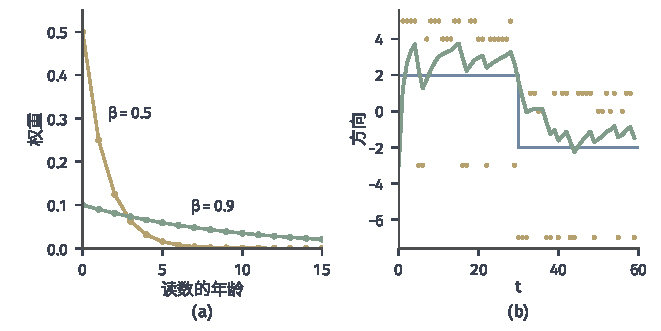
\includegraphics[width=112mm]{figures/05-optimization/05-stochastic-optimization/matplotlib/sgdb-momentum-track/figure.pdf}
  \caption{移动平均的平滑与滞后。(a)读数按年龄的权重$(1-\beta)\beta^{s}$，黄线$\beta=0.5$，绿线$\beta=0.9$。(b)蓝线是真实梯度，在$t=30$由$2$突变为$-2$；黄点是加上贯穿例噪声后的单次读数；绿线是$\beta=0.9$的移动平均方向（按权重之和归一化）。绿线的抖动比黄点小得多，但突变后要约十轮才转向。}
  \label{fig:sgdb-momentum-track}
\end{BookInlineFigure}

把两种效果算出来。先看平滑：设各轮读数的噪声相互独立，方差都是$\sigma^2$。移动平均的噪声部分是加权和，独立项的方差按权重平方相加，
\[
 (1-\beta)^2\sum_{s=0}^{t}\beta^{2s}\,\sigma^2
 =\frac{1-\beta}{1+\beta}\bigl(1-\beta^{2(t+1)}\bigr)\sigma^2 .
\]
于是轮数足够多时，方差缩小的倍数是
\begin{equation}
 \frac{1-\beta}{1+\beta}.
 \label{eq:sgdb-ema-noise}
\end{equation}

再看滞后：移动平均里读数的平均年龄是
\begin{equation}
 \sum_{s=0}^{\infty}s(1-\beta)\beta^{s}=\frac{\beta}{1-\beta}.
 \label{eq:sgdb-ema-age}
\end{equation}

取$\beta=0.9$，噪声方差缩小到约$0.053$倍，平均年龄却是$9$轮。图~\ref{fig:sgdb-momentum-track}(b)同时展示了两者：梯度不变时绿线紧贴真实值，梯度突变后绿线要约十轮才转向。这两个计算都假定噪声与位置无关，只说明趋势：真实运行中读数的位置本身受过去的噪声影响。

\paragraph{动量不是当前梯度的无偏估计}
读数条件无偏是说，固定历史后读数的均值等于当前梯度。动量方向并不继承这个性质。历史$\mathcal{F}^{(t)}$确定了$\bm{v}^{(t)}$，所以
\begin{equation}
 \mathbb{E}\bigl[\bm{v}^{(t+1)}\mid\mathcal{F}^{(t)}\bigr]=\beta\bm{v}^{(t)}+\bm{g}^{(t)},
 \label{eq:sgdb-hb-cond}
\end{equation}
只要$\bm{v}^{(t)}\neq\bm{0}$且$\beta>0$，它就不等于当前梯度$\bm{g}^{(t)}$。移动平均写法同样如此，条件均值是$\beta\bm{m}^{(t)}+(1-\beta)\bm{g}^{(t)}$。前面基于条件无偏的单步下降递推，不能把$\bm{v}^{(t+1)}$当成读数直接代入。

贯穿例给出具体的数。取$\alpha=0.1$，$\beta=0.5$，第一轮抽到第$3$项后位于$x^{(1)}=2.3$，速度是$v^{(1)}=-3$。此时三项梯度分别是$5.3,4.6,-2.1$，平均为$f'(2.3)=2.6$。第二轮的速度取$3.8$、$3.1$、$-3.6$三个值，条件均值是
\[
 \mathbb{E}\bigl[v^{(2)}\mid\mathcal{F}^{(1)}\bigr]=0.5\cdot(-3)+2.6=1.1\neq2.6.
\]

\paragraph{固定噪声下的稳态方差}
动量究竟能不能降低噪声的影响？在可以精确计算的情形中回答。考虑一元二次目标、加性噪声，下面的定理给出重球法长期的方差。

\begin{theorem}[加性噪声下重球法的稳态方差]
\label{thm:sgdb-hb-variance}
设$f(x)=\frac\lambda2x^2$，$\lambda>0$，读数为$\hat g^{(t)}=\lambda x^{(t)}+\xi^{(t)}$，其中$\xi^{(t)}$独立同分布，均值为零，方差为$\sigma^2$，且与此前的迭代独立。设$0\leq\beta<1$，$0<\alpha\lambda<2(1+\beta)$。则式~\eqref{eq:sgdb-hb}的迭代满足$\mathbb{E}x^{(t)}\to0$，并且
\begin{equation}
 \lim_{t\to\infty}\mathbb{E}\bigl[(x^{(t)})^2\bigr]
 =\frac{\alpha\sigma^2(1+\beta)}{\lambda(1-\beta)\bigl(2(1+\beta)-\alpha\lambda\bigr)}.
 \label{eq:sgdb-hb-variance}
\end{equation}
\end{theorem}

\begin{proof}
把式~\eqref{eq:sgdb-hb}写成二阶递推。令$a_1=1+\beta-\alpha\lambda$，$a_2=-\beta$，$s^2=\alpha^2\sigma^2$，则
\[
 x^{(t+1)}=a_1x^{(t)}+a_2x^{(t-1)}-\alpha\xi^{(t)}.
\]

特征方程是$r^2-a_1r-a_2=0$。条件$0\leq\beta<1$与$\lvert a_1\rvert<1+\beta$合起来保证两根都在单位圆内，这正是定理对$\alpha$和$\beta$的要求。所以均值的线性递推趋于零；二阶矩的线性递推的特征值是两根的两两乘积，也都在单位圆内，因而二阶矩收敛。记极限为
\[
 V_0=\lim_{t\to\infty}\mathbb{E}\bigl[(x^{(t)})^2\bigr],\qquad
 V_1=\lim_{t\to\infty}\mathbb{E}\bigl[x^{(t)}x^{(t-1)}\bigr].
\]

递推两边乘以$x^{(t)}$取期望。$\xi^{(t)}$与$x^{(t)}$独立且均值为零，噪声项消失；取极限得到$V_1=a_1V_0+a_2V_1$，也就是
\[
 V_1=\frac{a_1V_0}{1-a_2}.
\]

递推两边平方取期望，同样消去交叉项，取极限得到
\[
 V_0=(a_1^2+a_2^2)V_0+2a_1a_2V_1+s^2 .
\]

把$V_1$代入，两边乘以$1-a_2$并整理，$V_0$的系数变成
\[
 (1-a_2)(1-a_2^2)-a_1^2(1-a_2)-2a_1^2a_2
 =(1+a_2)\bigl[(1-a_2)^2-a_1^2\bigr].
\]

于是
\[
 V_0=\frac{s^2(1-a_2)}{(1+a_2)\bigl[(1-a_2)^2-a_1^2\bigr]}.
\]

代回$1-a_2=1+\beta$，$1+a_2=1-\beta$，以及
\[
 (1+\beta)^2-(1+\beta-\alpha\lambda)^2=\alpha\lambda\bigl(2(1+\beta)-\alpha\lambda\bigr),
\]
约去一个$\alpha\lambda$，即得式~\eqref{eq:sgdb-hb-variance}。
\end{proof}

看式~\eqref{eq:sgdb-hb-variance}怎样读。取$\beta=0$，它变成常步长随机梯度下降的$\alpha\sigma^2/(\lambda(2-\alpha\lambda))$。当$\alpha\lambda$远小于$1+\beta$时，$2(1+\beta)-\alpha\lambda\approx2(1+\beta)$，稳态方差约为
\begin{equation}
 \frac{\alpha\sigma^2}{2\lambda(1-\beta)}=\frac{\sigma^2}{2\lambda}\cdot\frac{\alpha}{1-\beta},
 \label{eq:sgdb-hb-small-step}
\end{equation}
只取决于有效步长$\alpha/(1-\beta)$。也就是说，步长很小时，动量的平滑效果恰好被有效步长的放大抵消：动量不改变噪声的稳态水平，它带来的是更快的初始收敛。

图~\ref{fig:sgdb-hb-floor}(b)验证了这一点：三个$\beta$的稳态目标差关于有效步长几乎是同一条线。图~\ref{fig:sgdb-hb-floor}(a)回到贯穿例，读数噪声随位置变化，定理的公式不再精确成立，但同样可以写出二阶矩的精确递推。$\alpha=0.1$，$\beta=0.5$的重球法稳态目标差约为$1.037$，有效步长相同的$\alpha=0.2$的随机梯度下降约为$1.217$，$\alpha=0.1$的随机梯度下降约为$0.528$。

\begin{BookInlineFigure}
  \centering
  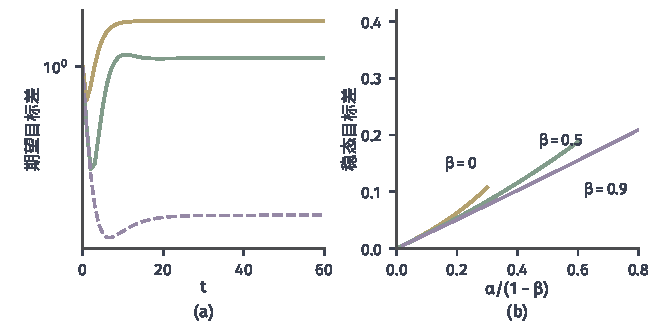
\includegraphics[width=112mm]{figures/05-optimization/05-stochastic-optimization/matplotlib/sgdb-hb-floor/figure.pdf}
  \caption{动量下的噪声残余。(a)贯穿例、$x^{(0)}=2$的期望目标差，由二阶矩的精确递推得到。绿线是$\alpha=0.1$，$\beta=0.5$的重球法；黄线是$\alpha=0.2$的随机梯度下降，有效步长与绿线相同；紫色虚线是$\alpha=0.1$的随机梯度下降。(b)式~\eqref{eq:sgdb-hb-variance}给出的稳态目标差$\frac\lambda2V_0$，$\lambda=2$，$\sigma^2=1$，横轴是有效步长。黄线、绿线、紫线分别取$\beta=0,0.5,0.9$，三条线的$\alpha$都取到$0.3$为止。}
  \label{fig:sgdb-hb-floor}
\end{BookInlineFigure}

\needspace{6\baselineskip}
\paragraph{变量}
\begin{itemize}
 \item $\bm{x}^{(t)}\in\mathbb{R}^n$：当前参数。
 \item $\bm{v}^{(t)}\in\mathbb{R}^n$：速度，形状与参数相同，是算法状态的一部分。
 \item $\hat{\bm g}^{(t)}\in\mathbb{R}^n$：当前点的随机读数。
 \item $\alpha>0$，$0\leq\beta<1$：固定的步长与动量系数。
 \item $T$：预定的总轮数。
\end{itemize}

\paragraph{初始化}
令$\bm{v}^{(0)}=\bm{0}$，第一轮没有历史，与一步随机梯度下降相同。例中是贯穿例的三项一元目标，取$\alpha=0.1$，$\beta=0.5$，读取顺序为第$3,1,2$项，起点和速度是
\[
 x^{(0)}=2,\qquad v^{(0)}=0.
\]

\needspace{6\baselineskip}
\paragraph{每轮更新}
在第$t$轮依次执行：
\begin{enumerate}
 \item \textbf{抽样并读取。}抽取下标$i^{(t)}$，在当前点读取$\hat{\bm g}^{(t)}$。这一步使用的是更新前的位置。例中第一轮抽到第$3$项，
 \[
  \hat g^{(0)}=f_3'(2)=-3.
 \]
 \item \textbf{更新速度。}按式~\eqref{eq:sgdb-hb-velocity}用旧速度和本轮读数计算$\bm{v}^{(t+1)}$。例中第一轮
 \[
  v^{(1)}=0.5\cdot0+(-3)=-3.
 \]
 \item \textbf{更新参数。}用新速度计算$\bm{x}^{(t+1)}$，然后$t\leftarrow t+1$。例中第一轮
 \[
  x^{(1)}=2-0.1\cdot(-3)=2.3.
 \]

 第二轮抽到第$1$项，读数和速度是
 \[
  \hat g^{(1)}=f_1'(2.3)=5.3,\qquad v^{(2)}=0.5\cdot(-3)+5.3=3.8,
 \]
 于是
 \[
  x^{(2)}=2.3-0.38=1.92.
 \]

 第三轮抽到第$2$项，读数和速度是
 \[
  \hat g^{(2)}=f_2'(1.92)=3.84,\qquad v^{(3)}=0.5\cdot3.8+3.84=5.74,
 \]
 于是
 \[
  x^{(3)}=1.92-0.574=1.346.
 \]
\end{enumerate}

单次读数的大小不能作为停止依据，这里按预定轮数结束。例中$T=3$，最终得到$x^{(3)}=1.346$，目标差为$(0.346)^2\approx0.120$。

\paragraph{保证与状态}
随机重球法每轮只多一个$n$维向量和一次向量加法，读取次数不变。恢复运行时必须同时恢复$\bm{v}^{(t)}$：只恢复参数，第一轮就退回了一步无动量的随机梯度下降。

一般目标上的保证要同时限定$\alpha$、$\beta$和读数的条件。定理~\ref{thm:sgdb-hb-variance}只针对二次目标和加性噪声。第~\ref{chap:first-order-methods}章已经看到，重球法在一般强凸光滑目标上，用二次目标的最优参数可能循环；随机读数不会修复这一点。分析时要把$(\bm{x}^{(t)},\bm{v}^{(t)})$作为一个整体，常用的做法是构造同时包含目标差和速度的势函数，递推中的噪声项按所选的势函数进入。

\subsection{随机Nesterov方法}
\label{sec:sgdb-nesterov}

\paragraph{主要思想}
第~\ref{chap:first-order-methods}章的Nesterov方法先沿动量探出去，到探出的位置再求梯度。随机版本的读数也放到这个前瞻点：
\begin{equation}
 \begin{aligned}
 \bm{y}^{(t)}&=\bm{x}^{(t)}+\beta\bigl(\bm{x}^{(t)}-\bm{x}^{(t-1)}\bigr),\\
 \bm{x}^{(t+1)}&=\bm{y}^{(t)}-\alpha\hat{\bm g}^{(t)},
 \end{aligned}
 \label{eq:sgdb-nag}
\end{equation}
这里$\hat{\bm g}^{(t)}$是在$\bm{y}^{(t)}$处读取的。图~\ref{fig:sgdb-state-order}把两种方法的状态次序并排画出。

\begin{BookInlineFigure}
  \centering
  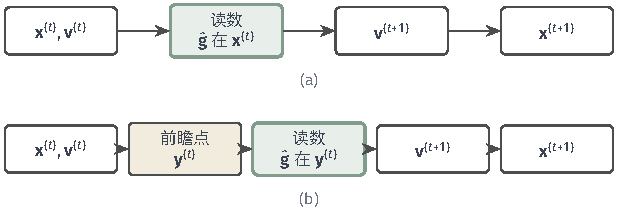
\includegraphics[width=104.64mm]{figures/05-optimization/05-stochastic-optimization/tikz/sgdb-state-order/figure.pdf}
  \caption{一轮内的状态次序。(a)随机重球法在当前点读数，接着更新速度和参数。(b)随机Nesterov方法先用历史算出前瞻点（黄），在前瞻点读数（绿），再更新速度和参数。两种方法的状态都是$(\bm{x}^{(t)},\bm{v}^{(t)})$，读取发生的位置不同。}
  \label{fig:sgdb-state-order}
\end{BookInlineFigure}

$\bm{y}^{(t)}$由抽样之前的量算出，所以固定历史后它是确定的。读数的条件无偏因而写成
\begin{equation}
 \mathbb{E}\bigl[\hat{\bm g}^{(t)}\mid\mathcal{F}^{(t)}\bigr]=\nabla f\bigl(\bm{y}^{(t)}\bigr).
 \label{eq:sgdb-nag-unbiased}
\end{equation}
这里被无偏估计的是前瞻点的梯度，不是$\bm{x}^{(t)}$处的梯度，两者一般不同。下面的比较把这一差别和其他差别列在一起。

\begin{BookInlineTable}
  \centering
  \caption{随机重球法与随机Nesterov方法的比较。}
  \label{tab:sgdb-momentum-compare}
  \begin{tabular}{lll}
    \toprule
    对比项 & 随机重球法 & 随机Nesterov方法\\
    \midrule
    读数位置 & 当前点$\bm{x}^{(t)}$ & 前瞻点$\bm{y}^{(t)}$\\
    条件无偏对象 & $\nabla f(\bm{x}^{(t)})$ & $\nabla f(\bm{y}^{(t)})$\\
    状态 & $\bm{x}^{(t)},\bm{v}^{(t)}$ & $\bm{x}^{(t)},\bm{v}^{(t)}$\\
    一般强凸光滑 & 最优参数可能循环 & 确定性时加速\\
    \bottomrule
  \end{tabular}
\end{BookInlineTable}

贯穿例中取同样的$\alpha=0.1$，$\beta=0.5$，读取顺序仍为第$3,1,2$项。三轮的前瞻点、读数和新位置分别是
\[
 \begin{aligned}
 y^{(0)}&=2, & \hat g^{(0)}&=-3, & x^{(1)}&=2.3,\\
 y^{(1)}&=2.45, & \hat g^{(1)}&=5.45, & x^{(2)}&=1.905,\\
 y^{(2)}&=1.7075, & \hat g^{(2)}&=3.415, & x^{(3)}&=1.366.
 \end{aligned}
\]

第二轮的读数$5.45$是$f_1'$在$y^{(1)}=2.45$处的值，而不是在$x^{(1)}=2.3$处的值。第三轮的前瞻点$1.7075$已经比$x^{(2)}=1.905$更靠近$x^\star=1$，读数相应变小。

\paragraph{方差怎样进入势函数}
确定性的Nesterov方法靠势函数证明加速。把梯度换成带噪声的读数，势函数的递推发生什么变化？下面的定理说明，收缩因子保留，但多了一个不随步数消失的噪声项。记号沿用第~\ref{chap:first-order-methods}章：$q=1/\sqrt\kappa$，以$\bm{u}^{(t)}$表示那里的辅助点。

\begin{theorem}[强凸情形下随机Nesterov方法的势函数递推]
\label{thm:sgdb-nag-noise}
设$f$的梯度$L$-Lipschitz连续且$\mu$强凸，$\mu>0$，最优解为$\bm{x}^\star$。取$\alpha=1/L$，$\beta=(1-q)/(1+q)$，$\bm{x}^{(-1)}=\bm{x}^{(0)}$。设前瞻点的读数满足
\begin{equation}
 \begin{gathered}
 \hat{\bm g}^{(t)}=\nabla f(\bm{y}^{(t)})+\bm{\xi}^{(t)},\\
 \mathbb{E}\bigl[\bm{\xi}^{(t)}\mid\mathcal{F}^{(t)}\bigr]=\bm{0},\qquad
 \mathbb{E}\bigl[\lVert\bm{\xi}^{(t)}\rVert_2^2\mid\mathcal{F}^{(t)}\bigr]\leq\sigma^2.
 \end{gathered}
 \label{eq:sgdb-nag-noise-condition}
\end{equation}
令$\bm{u}^{(0)}=\bm{x}^{(0)}$，并记
\begin{equation}
 \begin{aligned}
 \bm{u}^{(t+1)}&=\bm{x}^{(t)}+\frac1q\bigl(\bm{x}^{(t+1)}-\bm{x}^{(t)}\bigr),\\
 \Phi^{(t)}&=f(\bm{x}^{(t)})-f^\star+\frac\mu2\lVert\bm{u}^{(t)}-\bm{x}^\star\rVert_2^2.
 \end{aligned}
 \label{eq:sgdb-nag-potential}
\end{equation}
则
\begin{equation}
 \mathbb{E}\bigl[\Phi^{(t+1)}\mid\mathcal{F}^{(t)}\bigr]\leq(1-q)\Phi^{(t)}+\frac{\sigma^2}{L},
 \label{eq:sgdb-nag-recursion}
\end{equation}
因而
\begin{equation}
 \mathbb{E}f(\bm{x}^{(T)})-f^\star\leq(1-q)^T\Phi^{(0)}+\frac{\sqrt\kappa\,\sigma^2}{L}.
 \label{eq:sgdb-nag-bound}
\end{equation}
\end{theorem}

\begin{proof}
固定一步，省略上标$(t)$，记$\bm{g}=\nabla f(\bm{y})$，下一步的点记为$\bm{x}^+$和$\bm{u}^+$。

第一步，建立两个恒等式：
\[
 \bm{y}=\frac{\bm{x}+q\bm{u}}{1+q},\qquad
 \bm{u}^+=(1-q)\bm{u}+q\bm{y}-\frac q\mu\hat{\bm g}.
\]
这两个等式只用到更新形式$\bm{x}^+=\bm{y}-\hat{\bm g}/L$，读数是否带噪声不影响代数。第一式在$t=0$时成立，因为$\bm{y}^{(0)}=\bm{u}^{(0)}=\bm{x}^{(0)}$。设第一式对$t$成立，则$q\bm{u}=(1+q)\bm{y}-\bm{x}$，代入第二式右端，并用$q/\mu=1/(qL)$，得到
\[
 \frac1q\bigl(\bm{y}-\tfrac1L\hat{\bm g}-(1-q)\bm{x}\bigr)
 =\bm{x}+\frac1q(\bm{x}^+-\bm{x})=\bm{u}^+ .
\]

再由$\bm{u}^+$的定义和$\beta=(1-q)/(1+q)$，计算
\[
 \frac{\bm{x}^++q\bm{u}^+}{1+q}=\bm{x}^++\frac{1-q}{1+q}(\bm{x}^+-\bm{x})=\bm{y}^{(t+1)},
\]
所以第一式对$t+1$也成立。

第二步，函数项。由下降引理，
\[
 f(\bm{x}^+)\leq f(\bm{y})-\frac1L\langle\bm{g},\hat{\bm g}\rangle+\frac{1}{2L}\lVert\hat{\bm g}\rVert_2^2 .
\]

固定$\mathcal{F}^{(t)}$取条件期望。噪声的条件均值为零，交叉项消失，于是
\[
 \mathbb{E}\hat{\bm g}=\bm{g},\qquad
 \mathbb{E}\lVert\hat{\bm g}\rVert_2^2\leq\lVert\bm{g}\rVert_2^2+\sigma^2 .
\]

代入上式，得到
\[
 \mathbb{E}f(\bm{x}^+)\leq f(\bm{y})-\frac{1}{2L}\lVert\bm{g}\rVert_2^2+\frac{\sigma^2}{2L}.
\]

第三步，距离项。记$\bm{w}=(1-q)\bm{u}+q\bm{y}$，它由历史确定，$\bm{u}^+=\bm{w}-\frac q\mu\hat{\bm g}$。展开平方，用$q^2/(2\mu)=1/(2L)$，取条件期望，得到
\[
 \frac\mu2\mathbb{E}\lVert\bm{u}^+-\bm{x}^\star\rVert_2^2
 \leq\frac\mu2\lVert\bm{w}-\bm{x}^\star\rVert_2^2-q\langle\bm{g},\bm{w}-\bm{x}^\star\rangle+\frac{1}{2L}\bigl(\lVert\bm{g}\rVert_2^2+\sigma^2\bigr).
\]

第四步，相加。两式相加，$\lVert\bm{g}\rVert_2^2$相消，噪声项合计$\sigma^2/L$。剩下的部分完全由历史确定：
\[
 \mathbb{E}\Phi^{(t+1)}\leq f(\bm{y})-f^\star+\frac\mu2\lVert\bm{w}-\bm{x}^\star\rVert_2^2-q\langle\bm{g},\bm{w}-\bm{x}^\star\rangle+\frac{\sigma^2}{L}.
\]

第五步，处理确定部分，与精确梯度时相同。平方范数的凸性给出
\[
 \lVert\bm{w}-\bm{x}^\star\rVert_2^2\leq(1-q)\lVert\bm{u}-\bm{x}^\star\rVert_2^2+q\lVert\bm{y}-\bm{x}^\star\rVert_2^2 .
\]
把$\bm{w}-\bm{x}^\star$写成$(1-q)(\bm{u}-\bm{y})+(\bm{y}-\bm{x}^\star)$，并由强凸性得到
\[
 \langle\bm{g},\bm{y}-\bm{x}^\star\rangle\geq f(\bm{y})-f^\star+\frac\mu2\lVert\bm{y}-\bm{x}^\star\rVert_2^2 .
\]

两式代入后，$\lVert\bm{y}-\bm{x}^\star\rVert_2^2$项抵消，右端成为
\[
 (1-q)\bigl(f(\bm{y})-f^\star\bigr)+(1-q)\frac\mu2\lVert\bm{u}-\bm{x}^\star\rVert_2^2-q(1-q)\langle\bm{g},\bm{u}-\bm{y}\rangle+\frac{\sigma^2}{L}.
\]

第六步，由第一个恒等式，$q(\bm{u}-\bm{y})=\bm{y}-\bm{x}$，所以内积项等于$(1-q)\langle\bm{g},\bm{x}-\bm{y}\rangle$。凸性给出
\[
 \langle\bm{g},\bm{x}-\bm{y}\rangle\leq f(\bm{x})-f(\bm{y}),
\]
于是$f(\bm{y})$消去，得到式~\eqref{eq:sgdb-nag-recursion}。

最后对$t$取全期望并迭代，用$\sum_{j<T}(1-q)^j\leq1/q=\sqrt\kappa$，得到式~\eqref{eq:sgdb-nag-bound}。
\end{proof}

定理的两个条件起不同的作用。条件无偏保证了函数项和距离项中的一次项按精确梯度计算，这是用到式~\eqref{eq:sgdb-nag-noise-condition}第一式的地方。方差界让二次项多出$\sigma^2/(2L)$，函数项和距离项各一份。

与确定性结果的差别在于式~\eqref{eq:sgdb-nag-bound}最后一项。确定性时目标差按$(1-q)^T$收缩到零；有噪声时只能收缩到量级$\sqrt\kappa\sigma^2/L$的邻域，这一项不随$T$消失。所以确定性的加速界不能靠把梯度换成读数直接继承，要进一步下降就要改用更小的步长或增大批量，收缩因子也要随之调整。

式~\eqref{eq:sgdb-nag-bound}是上界，不同方法的上界不宜直接比较。在二次目标上可以写出精确的稳态值。图~\ref{fig:sgdb-accel-noise}用第~\ref{chap:first-order-methods}章的目标$f=(x_1^2+9x_2^2)/2$和起点$(9,1)$比较三种方法。无噪声时，重球法和Nesterov方法远快于梯度下降。加入方差为$1$的加性噪声后，梯度下降、重球法、Nesterov方法的稳态目标差分别约为$0.085$、$0.926$、$0.108$。重球法这组参数的有效步长是$1/3$，大于梯度下降的$1/9$；更重要的是$\lambda=9$时$\alpha\lambda=2.25$，已接近稳定边界$2(1+\beta)=2.5$，式~\eqref{eq:sgdb-hb-variance}的分母很小，噪声残余被放大约$11$倍。Nesterov方法的残余低于定理的上界$\sqrt\kappa\sigma^2/L=1/3$。

\begin{BookInlineFigure}
  \centering
  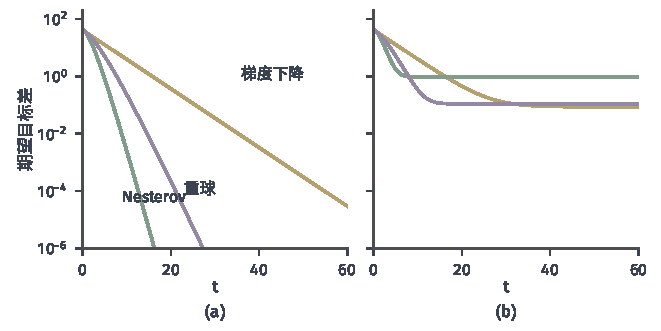
\includegraphics[width=112mm]{figures/05-optimization/05-stochastic-optimization/matplotlib/sgdb-accel-noise/figure.pdf}
  \caption{目标$f=(x_1^2+9x_2^2)/2$，起点$(9,1)$，由二阶矩的精确递推得到的期望目标差。(a)无噪声。(b)读数加上各分量方差为$1$的独立噪声。黄线是$\alpha=1/9$的梯度下降，绿线是$\alpha=\beta=1/4$的重球法，紫线是$\alpha=1/9$，$\beta=1/2$的Nesterov方法。加速缩短了初始阶段，重球法的稳态残余明显更高。}
  \label{fig:sgdb-accel-noise}
\end{BookInlineFigure}

\subsection{Lion符号动量（补充）}
\label{sec:sgdb-lion}

\paragraph{算法}
前两种方法的方向都保留读数的幅度。Lion只取方向的符号：把动量和本轮读数组成候选方向，逐坐标取符号，再按固定步长移动\scite{chen2023lion}。记$\operatorname{sign}(\cdot)$逐坐标作用。取$\bm{m}^{(0)}=\bm{0}$，系数$\beta_1,\beta_2\in[0,1)$，收缩系数$\gamma\geq0$，每轮读取$\hat{\bm g}^{(t)}$后依次计算候选方向和参数更新：
\begin{equation}
 \begin{aligned}
 \bm{c}^{(t)}&=\beta_1\bm{m}^{(t)}+(1-\beta_1)\hat{\bm g}^{(t)},\\
 \bm{x}^{(t+1)}&=\bm{x}^{(t)}-\alpha\operatorname{sign}\bigl(\bm{c}^{(t)}\bigr)-\alpha\gamma\bm{x}^{(t)}.
 \end{aligned}
 \label{eq:sgdb-lion}
\end{equation}

候选方向只参与这一步，下一轮用的动量由另一个系数单独记录：
\begin{equation}
 \bm{m}^{(t+1)}=\beta_2\bm{m}^{(t)}+(1-\beta_2)\hat{\bm g}^{(t)}.
 \label{eq:sgdb-lion-memory}
\end{equation}
$\beta_1$决定当前方向里旧动量占多少，$\beta_2$决定动量本身记忆多长，常见取值是$\beta_1=0.9$，$\beta_2=0.99$。因此读数在方向里的权重是$1-\beta_1$，在历史中的权重却是$1-\beta_2$，两者分开调节。

\paragraph{舍弃幅度}
符号操作舍弃了幅度。设候选方向是$\bm{c}=(0.1,3)$，同向但两个坐标相差$30$倍，取符号后是$(1,1)$，两个坐标移动相同的距离。图~\ref{fig:sgdb-lion-sign}(a)对比了这一点。优点是位移的大小完全由步长决定，读数的尺度和离群值都不会放大位移；缺点是信息少了，当前读数是否接近零，算法并不知道。

\begin{BookInlineFigure}
  \centering
  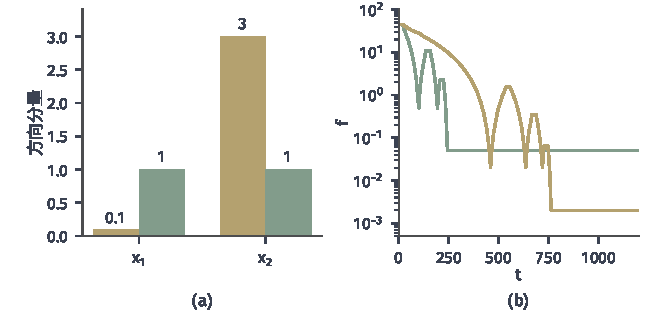
\includegraphics[width=112mm]{figures/05-optimization/05-stochastic-optimization/matplotlib/sgdb-lion-sign/figure.pdf}
  \caption{符号方向的效果。(a)候选方向$(0.1,3)$（黄）与其符号$(1,1)$（绿）。(b)目标$f=(x_1^2+9x_2^2)/2$上$\gamma=0$的Lion，使用精确梯度，纵轴是最近$20$轮内$f$的最大值。绿线$\alpha=0.1$，黄线$\alpha=0.02$。下降段之后曲线不再改善，平台高度随步长变化。}
  \label{fig:sgdb-lion-sign}
\end{BookInlineFigure}

\paragraph{贯穿例的三轮}
取$\alpha=0.1$，$\beta_1=0.9$，$\beta_2=0.99$，$\gamma=0$，$x^{(0)}=2$，$m^{(0)}=0$，读取顺序仍为第$3,1,2$项。三轮的读数、候选方向、新位置和新动量依次是
\[
 \begin{aligned}
 \hat g^{(0)}&=-3, & c^{(0)}&=-0.3, & x^{(1)}&=2.1, & m^{(1)}&=-0.03,\\
 \hat g^{(1)}&=5.1, & c^{(1)}&=0.483, & x^{(2)}&=2.0, & m^{(2)}&=0.0213,\\
 \hat g^{(2)}&=4, & c^{(2)}&=0.419, & x^{(3)}&=1.9, & m^{(3)}&=0.0611.
 \end{aligned}
\]

第一轮的候选方向由反向读数决定，参数上升；此后两轮都下降。读数的大小从$3$变到$5.1$，每轮的位移却都是$0.1$。

\paragraph{分别核对三个量}
第一个量是实际位移：$\gamma=0$时每个坐标的位移大小恰好是$\alpha$（候选方向该坐标非零时），不随读数减小。第二个量是原目标的残差。以$\beta_1=0$的一元精确梯度为例，每步的位移都是$\alpha$，迭代最后在距$x^\star$不超过$\alpha$的范围内来回，残差不会趋于零；$\beta_1>0$时候选方向有滞后，来回的范围由动量决定，同样不会随步数消失。图~\ref{fig:sgdb-lion-sign}(b)取$\beta_1=0.9$，$\beta_2=0.99$，平台的最高值在$\alpha=0.1$时是$0.05$，在$\alpha=0.02$时是$0.002$，减小残差要靠减小步长。

第三个量是参数收缩。$\gamma$项按更新前的参数做收缩，独立于读数和符号。它把参数往原点拉，不是原目标的下降方向，所以残差要按原目标$f$计算，不能把含收缩的位移当成$f$的下降。

\subsection{Muon矩阵动量（补充）}
\label{sec:sgdb-muon}

\paragraph{问题：把矩阵动量变换成更新方向}
参数是矩阵$\bm{W}\in\mathbb{R}^{m\times d}$时，动量$\bm{B}$也是矩阵。Lion逐元素地把幅度抹去，Muon在奇异方向上做类似的事：保留动量的奇异向量，把奇异值全部变成$1$\scite{jordan2024muon}。

这正是极分解所做的。矩形矩阵$\bm{B}$的紧奇异值分解是$\bm{B}=\bm{U}\bm{\Sigma}\bm{V}^\top$，极分解把它写成部分等距与半正定因子之积，
\begin{equation}
 \bm{B}=\bm{U}\bm{V}^\top\cdot\bm{V}\bm{\Sigma}\bm{V}^\top,\qquad
 \operatorname{orth}(\bm{B})=\bm{U}\bm{V}^\top .
 \label{eq:sgdb-polar}
\end{equation}
这里$\bm{U}\bm{V}^\top$就是\term{极因子}（polar factor），奇异向量与$\bm{B}$相同，奇异值全部是$1$。极分解的存在性和唯一性条件可参考\BookChapterRef{chap:polar-decomposition}{卷二第8章“极分解”}。

奇异值分解太贵，Muon用矩阵多项式的有限次迭代来近似极因子。设$\bm{X}=\bm{U}\bm{\Sigma}\bm{V}^\top$，对奇次多项式$p(\sigma)=\sum_jc_j\sigma^{2j+1}$，有
\begin{equation}
 \sum_jc_j\bm{X}\bigl(\bm{X}^\top\bm{X}\bigr)^j=\bm{U}\,p(\bm{\Sigma})\,\bm{V}^\top ,
 \label{eq:sgdb-odd-poly}
\end{equation}
所以这样的迭代不改变奇异向量，只对每个奇异值作用多项式。于是问题变成：选$p$，使得多次复合后所有奇异值都接近$1$。

\paragraph{算法次序}
一次更新的次序是：
\begin{enumerate}
 \item \textbf{读取。}在当前点（或前瞻点）得到矩阵读数$\hat{\bm G}^{(t)}$。
 \item \textbf{更新动量。}用旧动量和本轮读数计算
 \begin{equation}
  \bm{B}^{(t+1)}=\beta\bm{B}^{(t)}+\hat{\bm G}^{(t)}.
  \label{eq:sgdb-muon-momentum}
 \end{equation}
 \item \textbf{归一化。}用Frobenius范数除以动量，得到
 \[
  \bm{X}_0=\frac{\bm{B}^{(t+1)}}{\lVert\bm{B}^{(t+1)}\rVert_{\mathrm{F}}},
 \]
 所有非零奇异值落到$(0,1]$。
 \item \textbf{有限次迭代。}按多项式迭代$k$次，得到$\bm{X}_k$。
 \item \textbf{更新参数。}$\bm{W}^{(t+1)}=\bm{W}^{(t)}-\alpha\bm{X}_k$。
\end{enumerate}

经典的Newton--Schulz迭代取$p(\sigma)=\frac12(3\sigma-\sigma^3)$，矩阵形式是
\begin{equation}
 \bm{X}_{j+1}=\frac32\bm{X}_j-\frac12\bm{X}_j\bm{X}_j^\top\bm{X}_j .
 \label{eq:sgdb-newton-schulz}
\end{equation}
这个$p$有不动点$\sigma=1$，导数$p'(1)=0$，所以在$1$附近二阶收敛；对$\sigma\in(0,1]$迭代单调上升到$1$，起点离零很近时每步只放大约$1.5$倍。归一化保证了奇异值落在收敛区域里。

\paragraph{理想极因子与有限步近似}
用具体矩阵计算。取
\[
 \bm{B}=\begin{bmatrix}3&1\\1&3\end{bmatrix}.
\]
它的奇异值是$4,2$，奇异向量相同，极因子是单位矩阵$\bm{I}$。按Frobenius范数$\sqrt{20}$归一化后，奇异值是
\[
 0.894,\qquad 0.447.
\]

由式~\eqref{eq:sgdb-newton-schulz}迭代一次，两个奇异值变成$0.984$和$0.626$；迭代三次是$1.000$和$0.953$；迭代五次是$1.000$和$0.99998$，已经非常接近理想的极因子$\bm{I}$。图~\ref{fig:sgdb-muon-singular}(a)画出一般的$\sigma$：奇异值越小，需要的迭代次数越多。

\begin{BookInlineFigure}
  \centering
  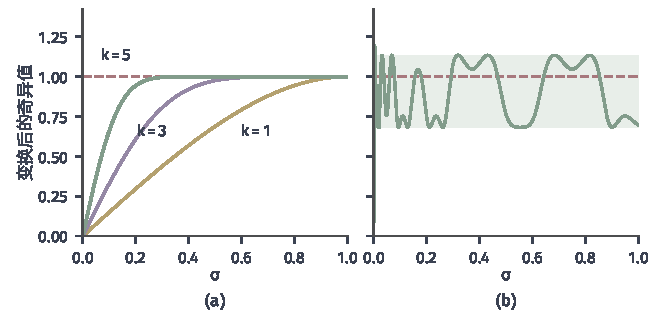
\includegraphics[width=112mm]{figures/05-optimization/05-stochastic-optimization/matplotlib/sgdb-muon-singular/figure.pdf}
  \caption{有限次迭代对奇异值的作用，横轴是归一化后的奇异值，红色虚线是理想的$1$。(a)经典Newton--Schulz迭代$k=1,3,5$次。(b)五次多项式$3.4445\sigma-4.7750\sigma^3+2.0315\sigma^5$复合$5$次，绿底是$\sigma\in[0.02,1]$上的取值范围，约为$[0.68,1.13]$。}
  \label{fig:sgdb-muon-singular}
\end{BookInlineFigure}

实际实现常用五次多项式\scite{jordan2024muon}：
\begin{equation}
 p(\sigma)=3.4445\,\sigma-4.7750\,\sigma^3+2.0315\,\sigma^5 .
 \label{eq:sgdb-muon-poly}
\end{equation}
它的系数是为“只迭代五次”专门选的。$p(1)=0.701$，$\sigma=1$不是它的不动点，继续迭代不会收敛到极因子。它的优势是小奇异值被放大得更快：在图~\ref{fig:sgdb-muon-singular}(b)中，$\sigma\in[0.02,1]$上五次复合后的值都落在约$[0.68,1.13]$内。

上面的矩阵用五次多项式迭代五次，奇异值变成$1.114$和$0.689$，与理想值$1$差得较远；两个奇异值之比从$2$缩小到约$1.6$。所以$\bm{X}_k$是对动量的尺度压缩，而不是精确的极因子。

\paragraph{计算成本与含义}
设$m\geq d$，先把$\bm{X}^\top\bm{X}$算出来。每次迭代做一次$\bm{X}^\top\bm{X}$、一次$(\bm{X}^\top\bm{X})^2$和一次$\bm{X}$右乘，运算量是$O(md^2)$；迭代$k$次合计$O(kmd^2)$。完整的奇异值分解也是这个量级，但常数更大。比较方法时，这部分要计入，每步的读取次数不变不等于每步成本不变。

动量矩阵和它的变换都只由梯度读数算出，其中没有二阶导数。奇异值变成$1$是对历史读数的幅度处理，它不是目标Hessian的近似。这种方法在什么问题上有效，只能在具体问题上由实际的目标值或验证指标判断。

\section{自适应更新}
\label{sec:sgdb-adaptive}

动量决定历史读数怎样合成方向。本节研究历史读数的另一种用途：根据过去读数的幅度，决定每个坐标或每个矩阵方向的更新尺度。不同坐标的读数幅度可能相差几个量级，同一个步长对它们不合适。这些方法都写成
\begin{equation}
 \bm{x}^{(t+1)}=\bm{x}^{(t)}-\alpha^{(t)}\bm{D}^{(t)}\hat{\bm g}^{(t)},
 \label{eq:sgdb-adaptive-form}
\end{equation}
或把$\hat{\bm g}^{(t)}$换成动量方向，其中$\bm{D}^{(t)}$是由历史读数算出的缩放。

$\bm{D}^{(t)}$的算法各不相同，但有一个共同的分析障碍：尺度和当前读数通常相关。如果$\bm{D}^{(t)}$在本轮抽样之前已经确定，它可以从条件期望中提到外面；这里不行，$\bm{D}^{(t)}$往往用到了本轮读数。一元的第一步最能说明问题。设累计统计用本轮读数，则第一步的方向是
\[
 \frac{\hat g}{\sqrt{\hat g^2}}=\operatorname{sign}(\hat g).
\]

在贯穿例的$x^{(0)}=2$处，三项读数是$5,4,-3$。缩放后的方向分别是$1,1,-1$，条件均值为
\[
 \frac13\bigl(1+1-1\bigr)=\frac13,
\]
而$f'(2)=2$。这个差别不是一个固定的比例因子：缩放后的条件均值由读数的分布决定，与$f'(2)$的大小没有固定关系。

所以下面每个方法都要写清统计量的更新次序，并分开说明保证所依赖的假设。全节沿用贯穿例的三轮读取，步长记作$\alpha$，稳定项$\epsilon>0$在手算中忽略。所有除法、平方根和乘方都逐坐标进行，$\odot$表示逐元素乘法。

\subsection{AdaGrad}
\label{sec:sgdb-adagrad}

\paragraph{累计平方与稀疏坐标}
设想一个分类问题，特征是某些词是否出现。常见词在几乎每个样本中出现，对应坐标的读数频繁非零；罕见词偶尔才出现。用同一个步长，罕见词的坐标几乎没有机会被更新。AdaGrad为每个坐标累计读数的平方，用它的平方根缩放当前读数\scite{duchi2011adagrad}。取$\bm{s}^{(0)}=\bm{0}$，读数之后先更新统计，再用新统计更新参数：
\begin{equation}
 \bm{s}^{(t+1)}=\bm{s}^{(t)}+\hat{\bm g}^{(t)}\odot\hat{\bm g}^{(t)},\qquad
 \bm{x}^{(t+1)}=\bm{x}^{(t)}-\alpha\frac{\hat{\bm g}^{(t)}}{\sqrt{\bm{s}^{(t+1)}}+\epsilon}.
 \label{eq:sgdb-adagrad}
\end{equation}

这里$\bm{s}$是累计统计，$\epsilon$只防止分母为零。第$j$个坐标的有效系数是$\alpha/(\sqrt{s_j^{(t+1)}}+\epsilon)$。读数频繁非零的坐标累计得快，系数缩小得快；稀疏坐标累计得慢，系数保持较大。

\paragraph{两个坐标的短序列}
下面用一个短序列计算有效系数。取$\alpha=1$，忽略$\epsilon$。坐标$1$每轮读数都是$1$，坐标$2$只在$t=0$和$t=3$读数为$1$，其余轮读数为零，不发生位移。表~\ref{tab:sgdb-adagrad-steps}列出每轮作用在非零读数上的系数。

\begin{BookInlineTable}
  \centering
  \caption{有效系数$\alpha/\sqrt{s_j^{(t+1)}}$的比较，$\alpha=1$，忽略稳定项。坐标$2$只在$t=0,3$读数为$1$，其余轮读数为零，记作“—”。RMSProp取$\rho=0.9$。}
  \label{tab:sgdb-adagrad-steps}
  \begin{tabular}{ccccc}
    \toprule
    & \multicolumn{2}{c}{AdaGrad} & \multicolumn{2}{c}{RMSProp}\\
    \cmidrule(lr){2-3}\cmidrule(lr){4-5}
    轮次$t$ & 坐标$1$ & 坐标$2$ & 坐标$1$ & 坐标$2$\\
    \midrule
    $0$ & $1.000$ & $1.000$ & $3.162$ & $3.162$\\
    $1$ & $0.707$ & — & $2.294$ & —\\
    $2$ & $0.577$ & — & $1.921$ & —\\
    $3$ & $0.500$ & $0.707$ & $1.705$ & $2.405$\\
    $4$ & $0.447$ & — & $1.563$ & —\\
    $5$ & $0.408$ & — & $1.461$ & —\\
    \bottomrule
  \end{tabular}
\end{BookInlineTable}

AdaGrad的两列中，坐标$1$的系数按$1/\sqrt{t+1}$持续缩小，到$t=3$是$0.5$；坐标$2$到$t=3$才累计了两次，系数是$0.707$。稀疏的坐标因此保留了较大的步长。

累计统计的问题是不会忘记旧尺度。设某坐标前$10$轮的读数幅度是$10$，之后幅度都是$1$。前$10$轮累计了$1000$，此后每轮只增加$1$，到第$80$轮累计量约为$1070$，系数约为$0.031$。图~\ref{fig:sgdb-adagrad-forget}(b)中的黄线显示了这一点：早期的大读数使有效系数永久偏小，算法可能在远离解时就几乎不再移动。

\begin{BookInlineFigure}
  \centering
  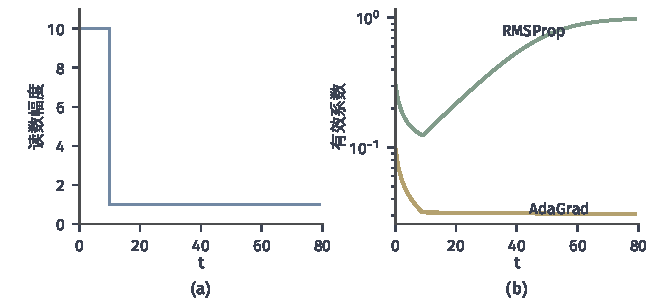
\includegraphics[width=112mm]{figures/05-optimization/05-stochastic-optimization/matplotlib/sgdb-adagrad-forget/figure.pdf}
  \caption{同一读数序列下的有效系数，$\alpha=1$，忽略稳定项。(a)读数幅度：前$10$轮为$10$，之后为$1$。(b)有效系数的对数图。黄线是AdaGrad，累计统计使系数一直偏小；绿线是$\rho=0.9$的RMSProp，大读数被遗忘后系数恢复到接近$1$。}
  \label{fig:sgdb-adagrad-forget}
\end{BookInlineFigure}

\paragraph{保证的范围}
AdaGrad的额外状态是一个$n$维向量，每轮额外计算量$O(n)$。保证按问题类型分别成立，引用时要注明。

\begin{itemize}
 \item 凸在线问题：对手依次给出凸损失，算法在有界可行域上行动，读数有界。评价对象是遗憾，也就是累计损失减去最好的固定决策的累计损失。原始分析给出$O(\sqrt T)$的遗憾，并在读数稀疏时有更好的常数\scite{duchi2011adagrad}。
 \item 随机凸问题：读数条件无偏时，可以由在线遗憾得到平均迭代的期望目标差，量级是$O(1/\sqrt T)$，同样需要有界可行域或相应的有界假设。
 \item 非凸光滑问题：评价对象是平方梯度范数的平均，需要读数有界或其他尾部条件，分母里的当前读数一般要特别处理。这类结果依赖具体的算法形式和假设，不能从凸的情形类推。
\end{itemize}

从更新形式本身推不出“比梯度下降快”。逐坐标缩放只有在问题的难点与坐标轴对齐时才有优势，图~\ref{fig:sgdb-adaptive-rotation}会展示这一边界。

\subsection{RMSProp}
\label{sec:sgdb-rmsprop}

\paragraph{用指数移动平均遗忘旧尺度}
AdaGrad难以遗忘，RMSProp把累计和换成\term{指数移动平均}（exponential moving average）\scite{hinton2012rmsprop}。取衰减系数$\rho\in[0,1)$，$\bm{s}^{(0)}=\bm{0}$：
\begin{equation}
 \bm{s}^{(t+1)}=\rho\bm{s}^{(t)}+(1-\rho)\hat{\bm g}^{(t)}\odot\hat{\bm g}^{(t)},\qquad
 \bm{x}^{(t+1)}=\bm{x}^{(t)}-\alpha\frac{\hat{\bm g}^{(t)}}{\sqrt{\bm{s}^{(t+1)}}+\epsilon}.
 \label{eq:sgdb-rmsprop}
\end{equation}

顺序与AdaGrad相同：先读，再用本轮读数更新$\bm{s}$，最后用新统计缩放本轮读数。$\epsilon$放在根号外，有的实现把它放在根号内，两者在分母很小时行为不同，记录实现时要写明。

展开递推，得到
\[
 \bm{s}^{(t+1)}=(1-\rho)\sum_{r=0}^{t}\rho^{t-r}\hat{\bm g}^{(r)}\odot\hat{\bm g}^{(r)}.
\]

$s$轮之前的读数平方的权重是$(1-\rho)\rho^{s}$，大约只记住最近$1/(1-\rho)$轮。$\rho=0.9$时约为$10$轮。

\paragraph{零初始化的早期偏差}
权重之和是$1-\rho^{t+1}$，早期小于$1$。读数恒为$g$时，
\[
 s^{(t+1)}=\bigl(1-\rho^{t+1}\bigr)g^2 ,
\]
早期分母偏小，有效系数偏大。表~\ref{tab:sgdb-adagrad-steps}的RMSProp列中，第一轮的系数是$1/\sqrt{0.1}\approx3.162$，比AdaGrad大得多。

再看图~\ref{fig:sgdb-adagrad-forget}的序列：前$10$轮把分母抬到约$8$，读数变小后，统计量大约以因子$\rho$逐轮衰减。第$30$轮的有效系数已经回到约$0.35$，第$79$轮约为$0.98$。

指数平均让尺度跟上最近的幅度，但它不提供一般的收敛保证。分母可能在大读数过后迅速变小，有效系数随之变大，下一节将看到这在特定问题上可能破坏收敛。

\subsection{Adam}
\label{sec:sgdb-adam}

\paragraph{主要思想}
RMSProp的分子只用当前读数。Adam在分子上也用移动平均，并修正两个平均的零初始化偏差\scite{kingma2015adam}。取$\beta_1,\beta_2\in[0,1)$，一阶统计$\bm{m}$与平方统计$\bm{s}$从零开始，读取本轮读数后依次计算
\begin{equation}
 \begin{aligned}
 \bm{m}^{(t+1)}&=\beta_1\bm{m}^{(t)}+(1-\beta_1)\hat{\bm g}^{(t)},\\
 \bm{s}^{(t+1)}&=\beta_2\bm{s}^{(t)}+(1-\beta_2)\hat{\bm g}^{(t)}\odot\hat{\bm g}^{(t)}.
 \end{aligned}
 \label{eq:sgdb-adam-stats}
\end{equation}

零初始化带来的偏差如何修正？展开$\bm{m}^{(t+1)}$，权重是$(1-\beta_1)\beta_1^{t-r}$，加起来是$1-\beta_1^{t+1}$，不是$1$。把统计量除以权重之和，得到两个修正量：
\begin{equation}
 \hat{\bm m}^{(t+1)}=\frac{\bm{m}^{(t+1)}}{1-\beta_1^{t+1}},\qquad
 \hat{\bm s}^{(t+1)}=\frac{\bm{s}^{(t+1)}}{1-\beta_2^{t+1}}.
 \label{eq:sgdb-adam-correction}
\end{equation}
读数恒为常数$\bm{g}$时，修正后$\hat{\bm m}^{(t+1)}=\bm{g}$，$\hat{\bm s}^{(t+1)}=\bm{g}\odot\bm{g}$，每一轮都恰好是常数读数的值。

参数更新使用修正后的量：
\begin{equation}
 \bm{x}^{(t+1)}=\bm{x}^{(t)}-\alpha\frac{\hat{\bm m}^{(t+1)}}{\sqrt{\hat{\bm s}^{(t+1)}}+\epsilon}.
 \label{eq:sgdb-adam-update}
\end{equation}

\begin{BookInlineFigure}
  \centering
  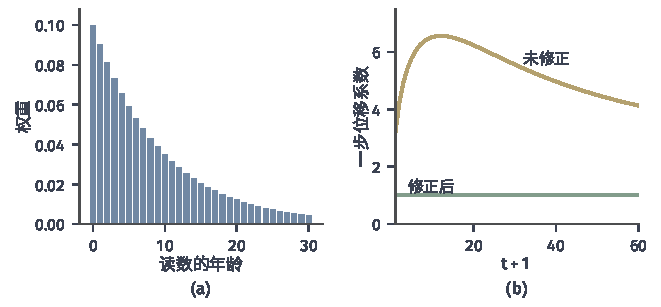
\includegraphics[width=112mm]{figures/05-optimization/05-stochastic-optimization/matplotlib/sgdb-adam-correction/figure.pdf}
  \caption{Adam的零初始化修正，$\beta_1=0.9$，$\beta_2=0.999$，读数恒为$1$，忽略稳定项。(a)$\bm{m}$的权重$(1-\beta_1)\beta_1^{s}$，$s$是读数的年龄。(b)一步位移的系数：黄线是未修正的$m/\sqrt{s}$，第一步约$3.16$，之后更大；绿线是修正后的$\hat m/\sqrt{\hat s}$，恒为$1$。}
  \label{fig:sgdb-adam-correction}
\end{BookInlineFigure}

图~\ref{fig:sgdb-adam-correction}(b)说明了修正的必要。$\beta_2$很接近$1$时，$\bm{s}$起步慢，未修正的$m/\sqrt{s}$在前几十轮都明显偏大，第$10$轮约为$6.5$。修正后系数恒为$1$。

\needspace{6\baselineskip}
\paragraph{变量}
\begin{itemize}
 \item $\bm{x}^{(t)}\in\mathbb{R}^n$：参数。
 \item $\bm{m}^{(t)},\bm{s}^{(t)}\in\mathbb{R}^n$：读数的一阶统计与平方统计。
 \item $t$：计时器，决定修正因子。
 \item $\alpha>0$，$\beta_1,\beta_2\in[0,1)$，$\epsilon>0$：步长、两个衰减系数、稳定项。
\end{itemize}

\paragraph{初始化}
令$\bm{m}^{(0)}=\bm{s}^{(0)}=\bm{0}$，$t=0$。例中是贯穿例的三项目标，取$\alpha=0.1$，$\beta_1=0.9$，$\beta_2=0.999$，读取顺序为第$3,1,2$项，手算时忽略$\epsilon$，起点和统计是
\[
 x^{(0)}=2,\qquad m^{(0)}=0,\qquad s^{(0)}=0.
\]

\needspace{6\baselineskip}
\paragraph{每轮更新}
在第$t$轮依次执行：
\begin{enumerate}
 \item \textbf{读取。}在当前点读取$\hat{\bm g}^{(t)}$。例中第一轮
 \[
  \hat g^{(0)}=f_3'(2)=-3.
 \]
 \item \textbf{更新统计。}按式~\eqref{eq:sgdb-adam-stats}计算$\bm{m}^{(t+1)}$和$\bm{s}^{(t+1)}$。例中第一轮
 \[
  m^{(1)}=0.1\cdot(-3)=-0.3,\qquad s^{(1)}=0.001\cdot9=0.009.
 \]
 \item \textbf{修正。}按式~\eqref{eq:sgdb-adam-correction}计算修正量。例中第一轮
 \[
  \hat m^{(1)}=\frac{-0.3}{0.1}=-3,\qquad \hat s^{(1)}=\frac{0.009}{0.001}=9.
 \]
 \item \textbf{更新参数。}按式~\eqref{eq:sgdb-adam-update}更新，然后$t\leftarrow t+1$。例中第一轮
 \[
  x^{(1)}=2-0.1\cdot\frac{-3}{3}=2.1.
 \]

 第二轮抽到第$1$项，读数和统计是
 \[
  \hat g^{(1)}=5.1,\qquad m^{(2)}=0.24,\qquad s^{(2)}=0.035001.
 \]
 两个修正分母是$1-0.81=0.19$和$1-0.998001=0.001999$，于是
 \[
  \hat m^{(2)}\approx1.2632,\qquad \hat s^{(2)}\approx17.509,\qquad \sqrt{\hat s^{(2)}}\approx4.184,
 \]
 参数更新为
 \[
  x^{(2)}=2.1-0.1\cdot\frac{1.2632}{4.184}\approx2.0698.
 \]

 第三轮抽到第$2$项，读数和统计是
 \[
  \hat g^{(2)}\approx4.1396,\qquad m^{(3)}\approx0.6300,\qquad s^{(3)}\approx0.052102.
 \]
 修正后
 \[
  \hat m^{(3)}\approx2.3246,\qquad \hat s^{(3)}\approx17.385,\qquad \sqrt{\hat s^{(3)}}\approx4.170,
 \]
 参数更新为
 \[
  x^{(3)}\approx2.0698-0.0558=2.0141.
 \]
\end{enumerate}

按预定轮数结束，例中$T=3$，最终得到$x^{(3)}\approx2.0141$。

\paragraph{修正偏差与优化方向的偏差}
修正因子只消除零初始化造成的权重不足，它不说明优化方向没有偏差。在上面的例子中，第二轮开始前$x^{(1)}=2.1$，$f'(2.1)=2.2$。固定历史后，$m^{(2)}$的条件均值是$0.9\cdot(-0.3)+0.1\cdot2.2=-0.05$，修正后的分子的条件均值约为
\[
 \frac{-0.05}{0.19}\approx-0.263 .
\]
它的符号甚至与$f'(2.1)$相反，原因是分子包含了上一轮的反向读数。分母还依赖本轮读数，所以式~\eqref{eq:sgdb-adam-update}的方向既不是当前梯度的无偏估计，也不是确定矩阵乘以当前梯度。

\paragraph{状态与保证}
Adam的状态包括$\bm{x}$、$\bm{m}$、$\bm{s}$和计时$t$。恢复运行时四项都要恢复：只恢复参数会丢失方向记忆；$t$错了，修正因子就错了。

Adam的原始论文给出了凸在线问题的分析，后来发现证明中存在问题，并有反例说明算法在一些凸问题上不收敛，下一小节说明这一点。引用Adam的保证时，必须对应具体的问题假设和参数设置，不能把一个具体分析中的结论当成算法的一般性质。

\paragraph{逐坐标缩放的边界}
图~\ref{fig:sgdb-adaptive-rotation}用精确梯度比较三种方法。目标是$f=(x_1^2+9x_2^2)/2$，起点$(9,1)$。主轴与坐标轴对齐时，AdaGrad第一步是$\alpha(1,1)$，随后逐坐标的尺度抵消了两个方向的曲率差异，到第$60$轮目标值约为$10^{-13}$。把目标和起点一起旋转$45^\circ$，陡峭方向不再对应一个坐标，AdaGrad到第$60$轮目标值约为$10^{-8}$，下降明显变慢。梯度下降对旋转不变，实线和虚线重合。

\begin{BookInlineFigure}
  \centering
  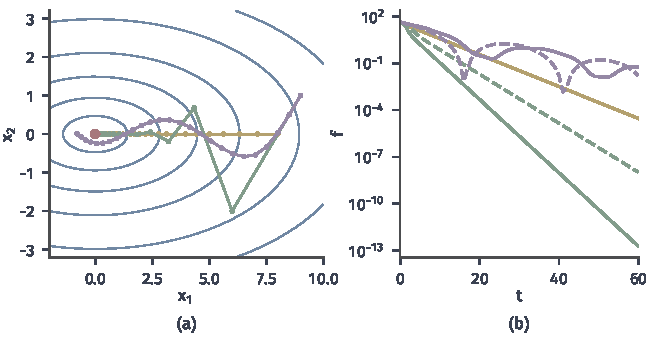
\includegraphics[width=112mm]{figures/05-optimization/05-stochastic-optimization/matplotlib/sgdb-adaptive-rotation/figure.pdf}
  \caption{逐坐标缩放与坐标系。目标$f=(x_1^2+9x_2^2)/2$，起点$(9,1)$，精确梯度。黄线是$\alpha=1/9$的梯度下降，绿线是$\alpha=3$的AdaGrad，紫线是$\alpha=0.5$的Adam（$\beta_1=0.9$，$\beta_2=0.999$）。(a)前$25$步的路径。(b)目标值：实线为原问题，虚线为把目标与起点一起旋转$45^\circ$后的同一问题，两条黄线重合。}
  \label{fig:sgdb-adaptive-rotation}
\end{BookInlineFigure}

\subsection{AMSGrad}
\label{sec:sgdb-amsgrad}

\paragraph{分母可能回落}
Adam和RMSProp的分母是指数平均，大读数过后可能迅速变小。分母一变小，有效步长就变大，此时的小读数被放大。这会造成什么后果？下面的构造说明，它足以让算法在一个凸问题上走向错误的方向\scite{reddi2018amsgrad}。

可行集是$[-1,1]$，读数依周期$3$变化，$C>2$：
\[
 \hat g^{(t)}=\begin{cases}C,& t\equiv1\pmod3,\\-1,&\text{其他}.\end{cases}
\]
对应的线性损失为$f_t(x)=\hat g^{(t)}x$，一个周期的总损失是$(C-2)x$，最优解是$x=-1$。取$C=3$，$\beta_1=0$（不用动量），$\beta_2=1/(1+C^2)=0.1$，步长$\alpha^{(t)}=0.1/\sqrt t$，更新后投影回$[-1,1]$。

\paragraph{一个周期内的净位移}
分母的三个值在稳态时循环。$s$按式~\eqref{eq:sgdb-adam-stats}递推，大读数$C$进入时升到约$8.207$，之后依次回落到$1.721$和$1.072$，所以一个周期的三个除数约为
\[
 \sqrt{8.207}\approx2.865,\qquad \sqrt{1.721}\approx1.312,\qquad \sqrt{1.072}\approx1.035.
\]
三步的位移与步长之比分别是$-3/2.865$，$+1/1.312$，$+1/1.035$，合计
\[
 -1.047+0.762+0.966=+0.681>0.
\]
一个周期的净位移是正的，迭代被推向错误的边界$x=+1$。大读数被大分母压低，小读数被回落的分母放大，方向信息就颠倒了。

\paragraph{算法}
AMSGrad让分母只增不减。分子和分母都不作零初始化修正，把历史最大的平方统计放进分母\scite{reddi2018amsgrad}。取$\bar{\bm s}^{(0)}=\bm{0}$，每轮在式~\eqref{eq:sgdb-adam-stats}之后计算
\begin{equation}
 \bar{\bm s}^{(t+1)}=\max\bigl\{\bar{\bm s}^{(t)},\bm{s}^{(t+1)}\bigr\},\qquad
 \bm{x}^{(t+1)}=\bm{x}^{(t)}-\alpha^{(t)}\frac{\bm{m}^{(t+1)}}{\sqrt{\bar{\bm s}^{(t+1)}}+\epsilon},
 \label{eq:sgdb-amsgrad}
\end{equation}
其中$\max$逐坐标取。

在上面的例子中，$\bar s$稳定在$8.207$，一个周期的位移与步长之比变为
\[
 \frac{-3+1+1}{2.865}\approx-0.349<0,
\]
净位移转为负，迭代走向$x=-1$。图~\ref{fig:sgdb-amsgrad-counter}的实际运行与此一致：Adam趋于$+1$，AMSGrad趋于$-1$。

\begin{BookInlineFigure}
  \centering
  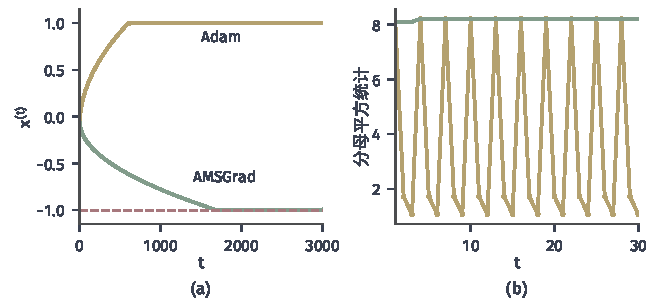
\includegraphics[width=112mm]{figures/05-optimization/05-stochastic-optimization/matplotlib/sgdb-amsgrad-counter/figure.pdf}
  \caption{周期线性目标上的Adam与AMSGrad，$C=3$，$\beta_1=0$，$\beta_2=0.1$，$\alpha^{(t)}=0.1/\sqrt t$，可行集$[-1,1]$。(a)迭代点，红色虚线是最优解$x=-1$。(b)分母中的平方统计：黄线是Adam随读数大幅涨落，绿线是AMSGrad保持最大值。}
  \label{fig:sgdb-amsgrad-counter}
\end{BookInlineFigure}

\paragraph{单调性是代数性质}
由更新规则，$\bar{\bm s}^{(t)}$逐坐标不减。若基步长$\alpha^{(t)}$不增，则每个坐标的有效缩放系数$\alpha^{(t)}/(\sqrt{\bar s_j^{(t)}}+\epsilon)$也不增。

这只是一个代数性质。它不说明目标值下降，也不说明算法收敛。AMSGrad的在线遗憾界需要凸性、有界可行域、有界读数，以及对$\beta_1^{(t)}$等参数的具体条件\scite{reddi2018amsgrad}；随机优化和非凸问题上的保证有各自的前提。不同问题上的结论不能互相代替。

\subsection{AdamW}
\label{sec:sgdb-adamw}

\paragraph{算法}
目标中常含平方惩罚$\frac\gamma2\lVert\bm{x}\rVert_2^2$。一种处理方式是把惩罚的梯度$\gamma\bm{x}$加到读数上，送进Adam的统计。另一种是\term{权重衰减}（weight decay）：历史统计只读取原目标的梯度，另外用更新前的参数单独收缩\scite{loshchilov2019adamw}。后一种方法称为AdamW，统计按式~\eqref{eq:sgdb-adam-stats}和式~\eqref{eq:sgdb-adam-correction}计算，参数更新改为
\begin{equation}
 \bm{x}^{(t+1)}=\bigl(1-\alpha^{(t)}\gamma\bigr)\bm{x}^{(t)}-\alpha^{(t)}\frac{\hat{\bm m}^{(t+1)}}{\sqrt{\hat{\bm s}^{(t+1)}}+\epsilon}.
 \label{eq:sgdb-adamw}
\end{equation}

收缩系数是$\alpha^{(t)}\gamma$，所以步长调度也带动收缩。对固定步长的随机梯度下降，两种做法相同：
\[
 \bm{x}-\alpha(\hat{\bm g}+\gamma\bm{x})=(1-\alpha\gamma)\bm{x}-\alpha\hat{\bm g}.
\]
但Adam的方向经过归一化，惩罚的梯度一旦进入统计，它的尺度也被归一化掉，两者不再相同。

\paragraph{同一标量首步比较}
取$x^{(0)}=1$，读数$\hat g^{(0)}=-0.1$，$\alpha=0.1$，$\gamma=0.5$，忽略$\epsilon$。第一轮的归一化方向等于读数的符号。AdamW用$\operatorname{sign}(-0.1)=-1$，按式~\eqref{eq:sgdb-adamw}，
\[
 x^{(1)}=(1-0.05)\cdot1+0.1=1.05.
\]

把惩罚梯度并入读数时，并入后的读数是$-0.1+0.5\cdot1=0.4$，符号变成$+1$，于是
\[
 x^{(1)}=1-0.1=0.9.
\]

两种做法的位移方向相反。图~\ref{fig:sgdb-adamw-step}显示了$\gamma$变化时的情况：AdamW的第一步关于$\gamma$连续变化；并入读数的做法在$\gamma=0.1$处突变，符号翻转后位移就不再随$\gamma$改变，惩罚的大小被归一化抹去了。

\begin{BookInlineFigure}
  \centering
  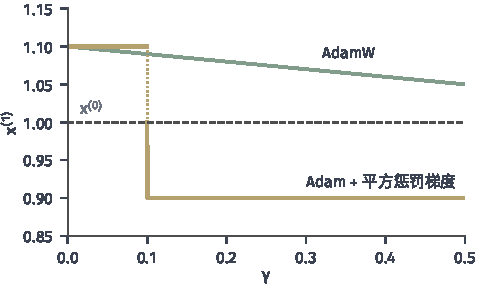
\includegraphics[width=82mm]{figures/05-optimization/05-stochastic-optimization/matplotlib/sgdb-adamw-step/figure.pdf}
  \caption{首步$x^{(1)}$关于惩罚系数$\gamma$的变化，$x^{(0)}=1$，$\hat g^{(0)}=-0.1$，$\alpha=0.1$。绿线是AdamW，黄线是把惩罚梯度并入读数后的Adam，虚线是起点。}
  \label{fig:sgdb-adamw-step}
\end{BookInlineFigure}

AdamW与平方惩罚并入读数的做法，优化的不是同一个迭代过程，它们停止的位置一般也不同。评价时要看实际定义的目标：返回点的目标值应写明是否包含惩罚项，收缩系数$\gamma$的含义也要随之说明。

\subsection{Adafactor统计压缩（补充）}
\label{sec:sgdb-adafactor}

\paragraph{用行列边际近似平方统计}
参数是矩阵$\bm{W}\in\mathbb{R}^{m\times d}$时，Adam的平方统计要存$md$个数。Adafactor只存平方统计的行和$\bm{r}\in\mathbb{R}^m$与列和$\bm{c}\in\mathbb{R}^d$，需要时重建近似的平方统计\scite{shazeer2018adafactor}。

设完整的平方统计是$\bm{V}$，$\bm{r}=\bm{V}\bm{1}_d$，$\bm{c}=\bm{V}^\top\bm{1}_m$。假定$\bm{V}$接近秩一，重建公式是
\begin{equation}
 \hat{\bm V}=\frac{\bm{r}\bm{c}^\top}{\bm{1}_m^\top\bm{r}} .
 \label{eq:sgdb-adafactor}
\end{equation}
分母是$\bm{V}$所有元素的和，这一归一化使重建保持行和与列和：$\hat{\bm V}\bm{1}_d=\bm{r}$，$\hat{\bm V}^\top\bm{1}_m=\bm{c}$。存储量从$md$降到$m+d$。

\paragraph{更新的次序}
一轮的次序是：先在读数的平方上加稳定项$\epsilon_1$，得到$\hat{\bm G}^{(t)}\odot\hat{\bm G}^{(t)}+\epsilon_1$，保证重建的分母为正；再分别用其行和与列和更新$\bm{r}$、$\bm{c}$的移动平均；然后由式~\eqref{eq:sgdb-adafactor}重建$\hat{\bm V}$；再求方向$\bm{Y}=\hat{\bm G}^{(t)}/\sqrt{\hat{\bm V}}$，把方向按均方根裁剪，最后乘以相对步长更新参数。相对步长与参数自身的均方根成正比，并有下界$\epsilon_2$。

这三件事分开算：统计压缩改变了尺度的来源，方向裁剪改变了方向的大小，相对步长改变了位移的量纲。评价改动带来的差别时，也要分别考虑。

\paragraph{保留与丢失的信息}
重建精确的条件很简单。若$\bm{V}$元素全为正，$\hat{\bm V}=\bm{V}$当且仅当$\bm{V}$秩为一，因为$\hat{\bm V}$按构造秩为一。例如
\[
 \bm{V}=\begin{bmatrix}1&2\\3&6\end{bmatrix}
\]
秩为一，行和是$(3,9)$，列和是$(4,8)$，总和是$12$，重建给出原矩阵。而
\[
 \bm{V}=\begin{bmatrix}4&1\\1&4\end{bmatrix}
\]
的行和、列和都是$(5,5)$，重建得到所有元素都是$2.5$的矩阵，对角线上的大值和非对角线的小值被抹平。

图~\ref{fig:sgdb-adafactor-recon}给出一个$6\times8$的例子。大尺度的行列结构被保留，逐元素的相对误差平均约为$0.13$，最大约为$0.70$。

\begin{BookInlineFigure}
  \centering
  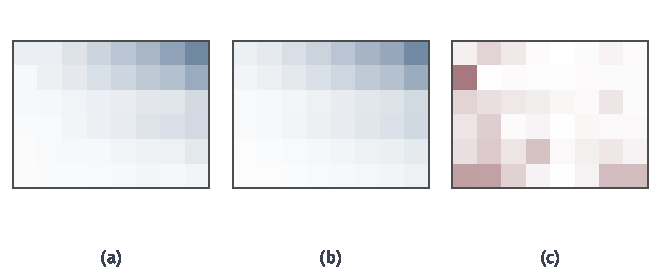
\includegraphics[width=112mm]{figures/05-optimization/05-stochastic-optimization/matplotlib/sgdb-adafactor-recon/figure.pdf}
  \caption{平方统计的行列压缩。(a)由$40$个随机读数算出的逐元素平方平均$\bm{V}$，形状$6\times8$。(b)按式~\eqref{eq:sgdb-adafactor}由$6$个行和与$8$个列和重建的$\hat{\bm V}$。(c)逐元素相对误差。颜色越深数值越大。}
  \label{fig:sgdb-adafactor-recon}
\end{BookInlineFigure}

压缩减少的只是统计的存储。参数、读数和方向仍是$md$个数；总计算量不会因此变成$O(m+d)$。低存储也不意味着收敛更快，近似的统计改变了方向，效果要回到目标上评价。

\subsection{Shampoo矩阵预条件（补充）}
\label{sec:sgdb-shampoo}

\paragraph{左右Gram统计}
逐坐标的尺度无法描述“某几行一起变化”这样的方向关系。Shampoo为矩阵参数维护左右两个Gram统计，分别刻画行空间和列空间方向的历史幅度\scite{gupta2018shampoo}。取$\epsilon>0$，$\bm{L}^{(0)}=\epsilon\bm{I}_m$，$\bm{R}^{(0)}=\epsilon\bm{I}_d$，读取矩阵读数$\hat{\bm G}^{(t)}$后先更新统计：
\begin{equation}
 \bm{L}^{(t+1)}=\bm{L}^{(t)}+\hat{\bm G}^{(t)}\hat{\bm G}^{(t)\top},\qquad
 \bm{R}^{(t+1)}=\bm{R}^{(t)}+\hat{\bm G}^{(t)\top}\hat{\bm G}^{(t)},
 \label{eq:sgdb-shampoo-stats}
\end{equation}
再用两侧的负四分之一次幂更新：
\begin{equation}
 \bm{W}^{(t+1)}=\bm{W}^{(t)}-\alpha\bigl(\bm{L}^{(t+1)}\bigr)^{-1/4}\hat{\bm G}^{(t)}\bigl(\bm{R}^{(t+1)}\bigr)^{-1/4}.
 \label{eq:sgdb-shampoo}
\end{equation}

$\epsilon$使两个统计正定，负四分之一次幂才有定义。按正交对角化计算：
\[
 \bm{L}=\bm{Q}\operatorname{diag}(\lambda_j)\bm{Q}^\top
 \quad\Longrightarrow\quad
 \bm{L}^{-1/4}=\bm{Q}\operatorname{diag}\bigl(\lambda_j^{-1/4}\bigr)\bm{Q}^\top .
\]
正交对角化可参考\BookChapterRef{chap:eigen-spectral-decomposition}{卷二第6章“谱分解”}。这两个矩阵是读数的累计，不是目标的Hessian。

\paragraph{单步：奇异值被拉平}
取$\epsilon\to0$，方阵可逆读数$\bm{G}=\bm{U}\bm{\Sigma}\bm{V}^\top$。则$\bm{G}\bm{G}^\top=\bm{U}\bm{\Sigma}^2\bm{U}^\top$，$\bm{G}^\top\bm{G}=\bm{V}\bm{\Sigma}^2\bm{V}^\top$，代入式~\eqref{eq:sgdb-shampoo}，
\[
 \bigl(\bm{G}\bm{G}^\top\bigr)^{-1/4}\bm{G}\bigl(\bm{G}^\top\bm{G}\bigr)^{-1/4}
 =\bm{U}\bm{\Sigma}^{-1/2}\bm{\Sigma}\bm{\Sigma}^{-1/2}\bm{V}^\top=\bm{U}\bm{V}^\top .
\]
一步的效果与Muon的理想极因子相同，所有奇异值都变成$1$。例如$\bm{G}=\operatorname{diag}(4,1/4)$时，两侧的变换都是$\operatorname{diag}(1/2,2)$，变换后得到$\bm{I}$，两个方向相差$16$倍的幅度被拉平。

累积多步之后不再这样简单。统计综合了历史上各方向的幅度，变换后的奇异值不等于$1$，并且随累积的读取逐渐减小，图~\ref{fig:sgdb-shampoo-flatten}(b)显示了这一点。这是累计式缩放的共同特点，与AdaGrad的有效系数逐渐减小相同。

\begin{BookInlineFigure}
  \centering
  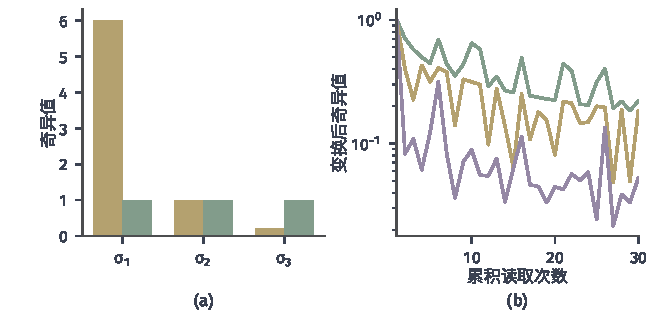
\includegraphics[width=112mm]{figures/05-optimization/05-stochastic-optimization/matplotlib/sgdb-shampoo-flatten/figure.pdf}
  \caption{Shampoo的奇异值变换，$\epsilon=10^{-6}$，$\bm{G}$是$3\times3$矩阵，奇异值为$6,1,0.2$。(a)单步：原始奇异值（黄）与式~\eqref{eq:sgdb-shampoo}变换后的奇异值（绿）。(b)累积读取时，变换后的三个奇异值随读取次数的变化，读数的各方向幅度随机变化。}
  \label{fig:sgdb-shampoo-flatten}
\end{BookInlineFigure}

\paragraph{计算成本}
Shampoo的额外成本比逐坐标方法高得多。统计的存储是$O(m^2+d^2)$；形成两个Gram矩阵需要$O(m^2d+md^2)$次运算；稠密谱分解求矩阵根一次约$O(m^3+d^3)$；两侧作用变换是$O(m^2d+md^2)$。

求根最贵，实际实现常隔若干步才重新计算根，中间继续使用旧因子。这样本轮使用的尺度来自若干步之前的统计，与式~\eqref{eq:sgdb-shampoo}“先更新后使用”不是同一个算法，记录时要写明刷新频率。比较方法时，统计存储、分解、旧因子的使用以及每步的乘法都要计入，不能只比较更新次数。

\section{梯度的处理}
\label{sec:sgdb-processing}

前两节的方向都由读数线性组合或缩放而来。本节研究更直接的改动：读数被截短、用有限精度算出、来自过去的点，甚至换成一个人为规定的向量。这些操作都使实际方向偏离原目标的梯度。

实际方向在什么点上、以什么误差近似当前梯度，这个误差怎样影响原目标上的进展？回答时把实际读数分解成三部分：真梯度$\bm{g}^{(t)}$、由历史确定的条件偏差$\bm{b}^{(t)}$、零条件均值的噪声$\bm{\xi}^{(t)}$，
\begin{equation}
 \hat{\bm g}^{(t)}=\bm{g}^{(t)}+\bm{b}^{(t)}+\bm{\xi}^{(t)},\qquad
 \mathbb{E}\bigl[\bm{\xi}^{(t)}\mid\mathcal{F}^{(t)}\bigr]=\bm{0}.
 \label{eq:sgdb-reading-decomposition}
\end{equation}

这个分解在前面的读数误差分析中已经用过，这里偏差项不再为零。下面分别看裁剪、近似和替代三种情形下$\bm{b}^{(t)}$从哪里来、能否被控制。

\subsection{梯度裁剪}
\label{sec:sgdb-clipping}

\paragraph{两种裁剪}
\term{梯度裁剪}（gradient clipping）在读数过大时把它截短，防止个别很大的读数把参数推得太远\scite{pascanu2013}。给定阈值$c>0$，有两种做法。\term{逐坐标裁剪}（coordinate-wise clipping）把每个坐标截到$[-c,c]$内：
\begin{equation}
 \bigl[\operatorname{clip}^{\mathrm{co}}_c(\bm{g})\bigr]_j=\max\{-c,\min\{c,g_j\}\}.
 \label{eq:sgdb-clip-coord}
\end{equation}

\term{范数裁剪}（norm clipping）整体缩放，只在范数超过阈值时起作用：
\begin{equation}
 \operatorname{clip}_c(\bm{g})=\bm{g}\cdot\min\Bigl\{1,\frac{c}{\lVert\bm{g}\rVert_2}\Bigr\}.
 \label{eq:sgdb-clip-norm}
\end{equation}

下面用同一个读数比较。取$\bm{g}=(3,4)$，$c=1$，两种裁剪的结果是
\[
 \operatorname{clip}^{\mathrm{co}}_1(\bm{g})=(1,1),\qquad
 \operatorname{clip}_1(\bm{g})=(0.6,0.8).
\]

前者的范数是$\sqrt2$，方向从与第一坐标轴夹角约$53^\circ$变成$45^\circ$；后者的范数是$1$，方向不变。图~\ref{fig:sgdb-clip-bias}(a)表明，逐坐标裁剪是投影到边长$2c$的正方形，范数裁剪是投影到半径$c$的圆盘。

\begin{BookInlineFigure}
  \centering
  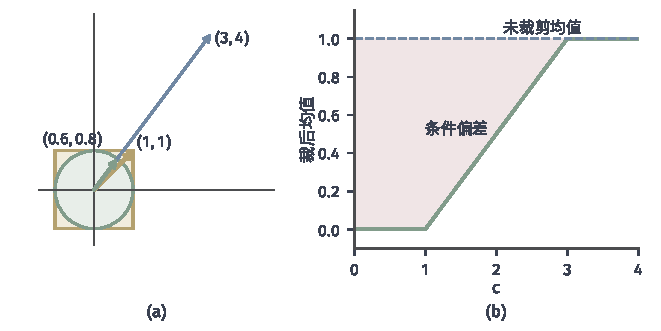
\includegraphics[width=112mm]{figures/05-optimization/05-stochastic-optimization/matplotlib/sgdb-clip-bias/figure.pdf}
  \caption{裁剪的几何与偏差。(a)读数$(3,4)$（蓝）在$c=1$时的两种裁剪：逐坐标裁剪得到黄色正方形角上的$(1,1)$；范数裁剪沿原方向缩到绿色圆上的$(0.6,0.8)$。(b)读数以相等概率取$3$或$-1$，绿线是逐点裁剪后的均值关于阈值$c$的变化，蓝色虚线是未裁剪的均值$1$，红色区域是两者之差。}
  \label{fig:sgdb-clip-bias}
\end{BookInlineFigure}

\paragraph{裁剪放在哪里}
一个算法中可以裁剪的位置不止一处，图~\ref{fig:sgdb-clip-position}标出了四处。裁剪位置$1$：裁剪逐样本读数后再平均，后面的动量和统计看到的都是裁过的量。裁剪位置$2$：先平均再裁剪批量读数。裁剪位置$3$：裁剪动量方向，统计仍记录原始读数。裁剪位置$4$：裁剪缩放后的方向，也就是最终的位移。

\begin{BookInlineFigure}
  \centering
  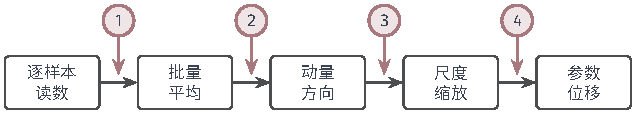
\includegraphics[width=107.64mm]{figures/05-optimization/05-stochastic-optimization/tikz/sgdb-clip-position/figure.pdf}
  \caption{更新流水线上可以施加裁剪的四个位置，圆圈内的数字对应正文的编号。位置不同，得到的是不同的算法，描述一次运行时要写明位置和阈值。}
  \label{fig:sgdb-clip-position}
\end{BookInlineFigure}

位置$1$和位置$2$的差别，用贯穿例在$x=2$处的三项读数说明。取$c=2$，全批量读数$5,4,-3$。先逐项裁剪再平均，得到
\[
 \frac13\bigl(2+2-2\bigr)=\frac23.
\]
先平均再裁剪，平均是$f'(2)=2$，未超过阈值，裁剪不起作用，得到$2$。前者有偏差，后者这里没有。

增大批量能否减小偏差，也取决于位置。逐样本裁剪后再平均，批量越大，平均越接近裁后读数的均值，偏差不随批量变小。先平均再裁剪时，批量越大，平均读数越集中在真梯度附近，只要真梯度的范数小于阈值，被裁剪的概率就越小，偏差随之减小。

\paragraph{用两点分布核对偏差}
裁剪是非线性运算，它改变读数的平均。设读数以相等概率取$3$与$-1$，均值为$1$。用$c=1$裁剪后，读数变为$1$与$-1$，均值为$0$：
\[
 \mathbb{E}\bigl[\operatorname{clip}_1(\hat g)\bigr]=0\neq1.
\]

条件偏差是$-1$，等于真梯度的相反数，方向信息完全消失。图~\ref{fig:sgdb-clip-bias}(b)画出裁后均值随阈值的变化：$c<1$时为$0$，$1\leq c<3$时为$(c-1)/2$，$c\geq3$时才恢复为$1$。

所以裁后的读数不能当作无偏梯度套用前面的定理。贯穿例能说明后果。取$c=2$的逐项裁剪，期望方向在$x=0$处为
\[
 \frac13\bigl(\operatorname{clip}_2(3)+\operatorname{clip}_2(0)+\operatorname{clip}_2(-9)\bigr)=\frac13(2+0-2)=0.
\]
也就是说，逐项裁剪的均值在$x=0$处恰好为零，而真正的最优点是$x^\star=1$，$f(0)-f^\star=1$。裁剪把期望更新的平衡点从$x=1$移到了$x=0$。

\paragraph{分别评价两种作用}
裁剪的作用要分开评价。第一是控制位移：范数裁剪在位置$2$或位置$4$保证每步位移的范数不超过$\alpha c$，这是确定的。第二是控制二阶矩：裁后读数的范数不超过$c$，所以它的二阶矩不超过$c^2$。原读数的二阶矩很大甚至无穷时，裁剪之后前面依赖方差假设的分析才可能使用。

这两种好处的代价是偏差$\bm{b}^{(t)}$。偏差怎样影响进展，由下一小节的递推回答。是否值得用偏差换取有界的二阶矩，要看具体的读数分布，没有无条件的结论。

\subsection{近似梯度}
\label{sec:sgdb-approximate}

\paragraph{几种来源}
实际得到的方向常常不是当前点的精确读数。下面三种情形都先问两件事：方向在哪个求值点上计算，误差能否由计算预算或步长控制。

第一是有限精度。例如浮点运算或内层线性方程只解到某个残差，读到的是$\nabla f(\bm{x}^{(t)})$的近似，误差$\bm{b}^{(t)}$的大小由内层的求解精度决定，增加每步计算可以使它变小。第二是量化，把读数的每个分量化到间距$\Delta$的格点上，$\lvert b_j\rvert\leq\Delta/2$，这是确定的偏差。真梯度比半个格子还小时，量化后的读数恰好是零，迭代会停在一个有残差的点上。第三是延迟读取，在第$t$轮用$\tau$轮之前的点上的梯度$\nabla f(\bm{x}^{(t-\tau)})$，也就是求值点不是当前点。

延迟的误差由步长控制，但可能破坏稳定性。设$f(x)=\frac12x^2$，用延迟$\tau=1$的精确梯度，
\[
 x^{(t+1)}=x^{(t)}-\alpha x^{(t-1)}.
\]
特征方程是$r^2-r+\alpha=0$。当$\alpha\in(0,1)$时，两根的模都小于$1$：两根为实数时积为$\alpha$，和为$1$，都在$(0,1)$内；两根共轭时模的平方等于积$\alpha$。当$\alpha=1$时两根落在单位圆上，迭代恰好以周期$6$循环。没有延迟时，$\alpha$可以取到$2$，所以延迟把稳定的步长范围缩小了一半。图~\ref{fig:sgdb-bias-delay}(b)是$\alpha=1$的情形，$\tau=2$时发散。

\begin{BookInlineFigure}
  \centering
  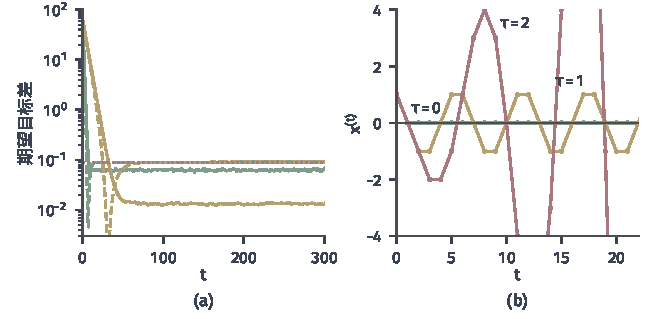
\includegraphics[width=112mm]{figures/05-optimization/05-stochastic-optimization/matplotlib/sgdb-bias-delay/figure.pdf}
  \caption{偏差、噪声与延迟的影响。(a)目标$f(x)=(x-1)^2+5$，初值$x=9$，$2000$次独立运行的平均目标差，绿线$\alpha=0.2$，黄线$\alpha=0.05$。实线是只有方差为$1$的噪声；虚线是只有常数偏差$b=0.6$，两种步长最终都停在红色点线$b^2/4=0.09$上。(b)目标$\frac12x^2$，$\alpha=1$，延迟$\tau=0,1,2$的迭代点。}
  \label{fig:sgdb-bias-delay}
\end{BookInlineFigure}

\paragraph{把偏差和噪声代入递推}
现在按式~\eqref{eq:sgdb-reading-decomposition}把两类误差代入有限步递推。下面的结果与前面的无偏分析结构相同，只多了偏差产生的一项。

\begin{theorem}[有偏读数下的平均平方梯度范数]
\label{thm:sgdb-biased}
设$f$梯度$L$-Lipschitz连续，下确界为$f_{\inf}$。设读数满足式~\eqref{eq:sgdb-reading-decomposition}，其中$\bm{b}^{(t)}$由$\mathcal{F}^{(t)}$确定，并且
\begin{equation}
 \lVert\bm{b}^{(t)}\rVert_2\leq B,\qquad
 \mathbb{E}\bigl[\lVert\bm{\xi}^{(t)}\rVert_2^2\mid\mathcal{F}^{(t)}\bigr]\leq\sigma^2 .
 \label{eq:sgdb-biased-condition}
\end{equation}
取固定步长$0<\alpha\leq1/L$，用$\hat{\bm g}^{(t)}$代替梯度做一步更新。则
\begin{equation}
 \mathbb{E}\bigl[f(\bm{x}^{(t+1)})\mid\mathcal{F}^{(t)}\bigr]\leq f(\bm{x}^{(t)})-\frac\alpha2\lVert\bm{g}^{(t)}\rVert_2^2+\frac\alpha2B^2+\frac{L\alpha^2}{2}\sigma^2,
 \label{eq:sgdb-biased-step}
\end{equation}
因而
\begin{equation}
 \frac1T\sum_{t=0}^{T-1}\mathbb{E}\lVert\bm{g}^{(t)}\rVert_2^2\leq\frac{2\bigl(f(\bm{x}^{(0)})-f_{\inf}\bigr)}{\alpha T}+B^2+L\alpha\sigma^2 .
 \label{eq:sgdb-biased-bound}
\end{equation}
\end{theorem}

\begin{proof}
由下降引理，
\[
 f(\bm{x}^{(t+1)})\leq f(\bm{x}^{(t)})-\alpha\langle\bm{g}^{(t)},\hat{\bm g}^{(t)}\rangle+\frac{L\alpha^2}{2}\lVert\hat{\bm g}^{(t)}\rVert_2^2 .
\]

记$\bm{a}=\bm{g}^{(t)}+\bm{b}^{(t)}$，它由历史确定。固定$\mathcal{F}^{(t)}$取条件期望。噪声的条件均值为零，所以交叉项消失，
\[
 \mathbb{E}\langle\bm{g}^{(t)},\hat{\bm g}^{(t)}\rangle=\langle\bm{g}^{(t)},\bm{a}\rangle,\qquad
 \mathbb{E}\lVert\hat{\bm g}^{(t)}\rVert_2^2\leq\lVert\bm{a}\rVert_2^2+\sigma^2 .
\]

由$\alpha\leq1/L$，$L\alpha^2/2\leq\alpha/2$，于是$\lVert\bm{a}\rVert_2^2$前的系数可以放大到$\alpha/2$，得到
\[
 \mathbb{E}f(\bm{x}^{(t+1)})\leq f(\bm{x}^{(t)})-\alpha\langle\bm{g}^{(t)},\bm{a}\rangle+\frac\alpha2\lVert\bm{a}\rVert_2^2+\frac{L\alpha^2}{2}\sigma^2 .
\]

展开平方并配方，
\[
 -\alpha\langle\bm{g}^{(t)},\bm{a}\rangle+\frac\alpha2\lVert\bm{a}\rVert_2^2
 =\frac\alpha2\bigl(\lVert\bm{a}-\bm{g}^{(t)}\rVert_2^2-\lVert\bm{g}^{(t)}\rVert_2^2\bigr)
 =\frac\alpha2\bigl(\lVert\bm{b}^{(t)}\rVert_2^2-\lVert\bm{g}^{(t)}\rVert_2^2\bigr).
\]

代入$\lVert\bm{b}^{(t)}\rVert_2\leq B$，得到式~\eqref{eq:sgdb-biased-step}。对$t=0,\ldots,T-1$取全期望并累加，用$f(\bm{x}^{(T)})\geq f_{\inf}$，两边除以$\alpha T/2$，得到式~\eqref{eq:sgdb-biased-bound}。
\end{proof}

式~\eqref{eq:sgdb-biased-bound}有三项。第一项是初始误差，随$T$消失。第三项是噪声，正比于$\alpha$，可以用小步长或小批量压低。第二项$B^2$既不依赖$\alpha$，也不依赖$T$。

图~\ref{fig:sgdb-bias-delay}(a)验证了这一分工。只有噪声时，$\alpha$从$0.2$减到$0.05$，平台约从$0.0625$降到$0.0132$，与$\alpha/(2(2-2\alpha))$一致。只有常数偏差时，两种步长最终停在同一高度$b^2/4=0.09$，小步长只是到达得更慢。

\paragraph{上界中的残余不是下限}
$B^2$是上界中的项，不是误差的下限。偏差项能否真的造成残余，取决于偏差的结构。

设$f(x)=\frac12x^2$，常数偏差$b$使读数的均值变成$x+b$，迭代的平衡点是$x=-b$，平方梯度是$b^2$，这时界是紧的。如果偏差随梯度变小，满足
\[
 \lVert\bm{b}^{(t)}\rVert_2\leq\rho\lVert\bm{g}^{(t)}\rVert_2,\qquad\rho<1,
\]
回到证明中的配方等式，确定部分的下降量至少是$\frac\alpha2(1-\rho^2)\lVert\bm{g}^{(t)}\rVert_2^2$，平方梯度可以趋于零。裁剪在读数范数以概率$1$小于阈值时偏差恰好为零，这时实际残余也小于用$B^2$估计的量。

\subsection{替代梯度（补充）}
\label{sec:sgdb-surrogate}

\paragraph{导数没有用处的前向函数}
前向函数有时是分段常数，经典梯度几乎处处为零。设$Q(w)=\lfloor w+\tfrac12\rfloor$是取整，损失为
\begin{equation}
 F(w)=\frac12\bigl(Q(w)-a\bigr)^2 .
 \label{eq:sgdb-rounding}
\end{equation}

$Q$在非半整数点局部为常数，所以除了可数个跳跃点外$F'(w)=0$，导数不提供任何信息。梯度下降一步也不会动。

\paragraph{人为指定的反向规则}
\term{直通估计}（straight-through estimator）在反向计算时假装$Q$是恒等映射，规定$\mathrm{d}Q/\mathrm{d}w=1$\scite{math-bengio2013estimating}，返回的方向是
\begin{equation}
 g_{\mathrm{STE}}(w)=Q(w)-a .
 \label{eq:sgdb-ste}
\end{equation}

这类人为指定的方向统称\term{替代梯度}（surrogate gradient）。要区分两件事：前向函数$F$是实际被评价的对象，反向规则是另外选的方向生成方式，两者之间没有求导关系。在计算图中还常用\term{停止梯度}（stop-gradient）这一传播规则写成$w+\operatorname{sg}(Q(w)-w)$，其中$\operatorname{sg}$前向原样传值，反向阻断传播；前向得到$Q(w)$，反向等于恒等映射。它是计算图上的规则，不是数学运算的导数。

\paragraph{跨阈值的两次更新}
图~\ref{fig:sgdb-ste-round}给出同一点出发的两个结果。取$w=0.3$，此时$Q(w)=0$。若$a=1$，损失是$F=0.5$，替代方向是$-1$，取步长$0.4$走到$w=0.7$，此时$Q=1$，损失降到
\[
 F(0.7)=\frac12(1-1)^2=0.
\]

若$a=0.3$，损失是$F=0.045$，替代方向是$-0.3$，取步长$4/3$同样走到$w=0.7$，损失却升到
\[
 F(0.7)=\frac12(1-0.3)^2=0.245.
\]

光滑情形下的下降依赖于“小步之内一阶模型准确”，而跨过跳跃点时一阶模型完全失效。所以无法从替代方向推出下降。

\begin{BookInlineFigure}
  \centering
  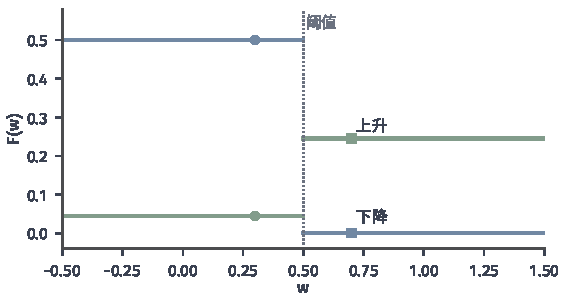
\includegraphics[width=96mm]{figures/05-optimization/05-stochastic-optimization/matplotlib/sgdb-ste-round/figure.pdf}
  \caption{取整前向上的直通更新。蓝线$F(w)=\frac12(Q(w)-1)^2$，绿线$F(w)=\frac12(Q(w)-0.3)^2$，都是分段常数，点线是取整阈值$w=0.5$。圆点是起点$w=0.3$，方块是走一步后的$w=0.7$：蓝色的损失由$0.5$降到$0$，绿色的损失由$0.045$升到$0.245$。}
  \label{fig:sgdb-ste-round}
\end{BookInlineFigure}

\paragraph{替代方向的地位}
替代方向既不是原目标的经典梯度，一般也不是凸次梯度。以$a=1$，$w=0.3$为例，若$s$是全局次梯度，要求不等式$F(y)\geq F(0.3)+s(y-0.3)$对一切$y$成立。

取$y=0.7$，得到$0\geq0.5+0.4s$，即$s\leq-1.25$。取$y=-0.4$，$F(-0.4)=0.5$，得到$s\geq0$。两者矛盾，这样的$s$不存在，$F$在该点没有全局次梯度，$-1$更不是。局部上$F$在该点附近为常数，局部的次梯度只有$0$，也不是$-1$。

所以使用替代方向的算法，只能回到实际的前向目标上评价。比较的量应是前向损失或原问题的目标值，停止准则也应基于前向量，而不是替代方向的范数是否变小。

\section{误差与计算成本}
\label{sec:sgdb-cost}

本章已经出现了很多方法，每一种都有自己的误差界和成本描述。它们能不能放在一起比较？回答这个问题，先要固定三件事：要最小化哪个目标，算法返回什么，用什么量计算成本。本节依次讨论评价对象、总计算成本，以及当输入的数据发生变化时算法的有限步响应。

\subsection{误差的评价对象}
\label{sec:sgdb-error-objects}

\paragraph{量与返回点的配对}
一个收敛结论由两部分组成：度量什么量，度量哪个点。常用的量有目标差、到最小点的距离、梯度范数或邻近残差；常用的返回点有最后一点、平均点和随机返回点。量和点的配对不能互换，表~\ref{tab:sgdb-error-pairing}列出常见的配对。

\begin{BookInlineTable}
  \centering
  \caption{常见的误差量与返回点的配对。条件只列出主要假设，具体常数和步长以相应结论为准。}
  \label{tab:sgdb-error-pairing}
  \begin{tabular}{lll}
    \toprule
    误差量 & 返回点 & 主要条件\\
    \midrule
    期望目标差 & 加权平均点 & 凸\\
    期望目标差 & 最后一点 & 强凸\\
    到最小点的距离 & 最后一点 & 强凸\\
    平方梯度范数 & 按权重随机返回 & 光滑非凸\\
    邻近残差 & 按权重随机返回 & 复合目标\\
    \bottomrule
  \end{tabular}
\end{BookInlineTable}

配对的差别可以在贯穿例上看见。常步长$\alpha=0.1$时，随机梯度下降的最后一点的期望目标差趋于$0.528$，不随轮数继续下降。模拟$20$万条路径，后$2000$轮的平均点的期望目标差约为$0.0024$，比最后一点小两个多量级。平均减小了噪声，但关于平均点的界不能直接移用到某个单独的迭代点上。

\paragraph{期望保证与概率保证}
上面的误差界都是期望。期望小不等于每次运行都小。若$Z\geq0$是目标差，$\mathbb{E}Z\leq\varepsilon$，由Markov不等式，对任意$\delta\in(0,1)$，
\begin{equation}
 \mathbb{P}\Bigl(Z\geq\frac{\varepsilon}{\delta}\Bigr)\leq\delta .
 \label{eq:sgdb-markov}
\end{equation}

比如$\mathbb{E}Z\leq0.01$，只能得到目标差超过$0.1$的概率不超过$0.1$。这里$\varepsilon/\delta$随$\delta$变小放大得很快。更强的高概率保证需要读数的尾部条件，例如有界或次高斯，并使用鞅集中不等式，推导要用到鞅的工具，这里只说明它与期望保证的区别。

路径的长期性质是另一个问题，例如一条路径是否几乎必然收敛，这类结论依赖步长条件和鞅收敛定理，属于前面提到的长期路径分析。有限步的期望界不能回答这个问题。

\paragraph{各类误差进入递推的位置}
本章遇到的误差进入递推的不同位置。条件噪声进入二次项，贡献$\sigma^2$乘以步长的相应幂次，能靠减小步长或增大批量压低。系统偏差进入一次项，贡献的$B^2$不随步长变小。近似求解的误差与偏差类似，由内层精度决定。

这些都是\term{优化误差}（optimization error），针对的是给定的目标。如果目标是由一批样本构造的有限和，而真正关心的是总体上的目标，那么还有一部分由样本有限造成的差距。这部分属于统计误差，优化再精确也不能消除，分析它需要样本数和分布条件。优化误差不能代替统计误差，反过来也一样。

\subsection{总计算成本}
\label{sec:sgdb-total-cost}

\paragraph{统一单位}
比较方法之前，先把计量单位统一下来。常用的单位有样本梯度读取次数、参数更新次数、完整遍历次数。一次全梯度是$N$次样本梯度读取；一轮批量大小为$b$的小批量是$b$次读取、一次更新。此外要把快照、梯度表、矩阵分解、邻近求解、同步统计这些额外工作计入。

下面的估计都假定目标在同一种归一化下，要求同一个精度$\varepsilon$，略去常数因子。设$f$是$N$项的平均，强凸常数$\mu$，整体光滑常数$L$，逐项光滑常数最大值$L_{\max}$，$\kappa_{\max}=L_{\max}/\mu$，读数方差$\sigma^2$。

\begin{BookInlineTable}
  \centering
  \caption{强凸有限和目标上达到目标差$\varepsilon$的样本梯度读取量，略去常数因子。}
  \label{tab:sgdb-cost-table}
  \begin{tabular}{lll}
    \toprule
    方法 & 读取量 & 额外状态\\
    \midrule
    全梯度下降 & $N\kappa\ln(1/\varepsilon)$ & 无\\
    随机梯度下降 & $\sigma^2/(\mu\varepsilon)$ & 无\\
    SVRG & $(N+\kappa_{\max})\ln(1/\varepsilon)$ & 一个快照\\
    SAGA & $(N+\kappa_{\max})\ln(1/\varepsilon)$ & 梯度表，$N$份\\
    \bottomrule
  \end{tabular}
\end{BookInlineTable}

用具体数比较。取$N=1000$，$\kappa=\kappa_{\max}=100$，$\sigma^2/\mu=1$。

当$\varepsilon=10^{-3}$时，$\ln(1/\varepsilon)\approx6.9$，全梯度下降、随机梯度下降和SVRG的读取量分别是
\[
 6.9\times10^{5},\qquad 1000,\qquad 7.6\times10^{3},
\]
随机梯度下降最便宜。当$\varepsilon=10^{-6}$时，$\ln(1/\varepsilon)\approx13.8$，三个读取量变成
\[
 1.4\times10^{6},\qquad 10^{6},\qquad 1.5\times10^{4},
\]
SVRG的读取量比随机梯度下降少约$60$倍。结论是：用什么方法取决于要求的精度，低精度时常步长的简单方法足够，高精度时方差减小的方法更划算。

\paragraph{按不同单位，排序不同}
图~\ref{fig:sgdb-cost-units}在同一个最小二乘问题上用两种单位画出四种方法。按参数更新次数，全梯度下降明显最快，因为每次更新读了全部$200$项。按样本读取量，全梯度下降落到后面，SAGA和随机梯度下降早期下降最快。只按外层轮数排序，或者只按更新次数排序，都会得出不同的结论。

\begin{BookInlineFigure}
  \centering
  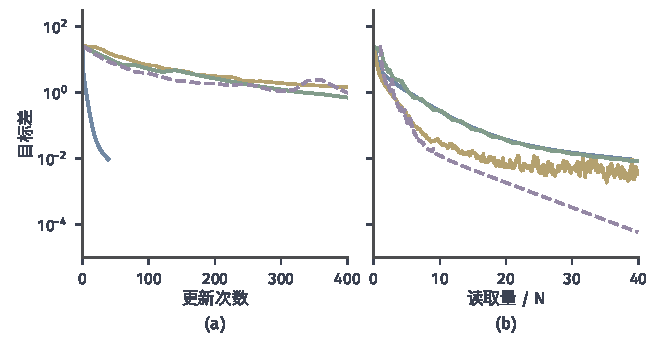
\includegraphics[width=112mm]{figures/05-optimization/05-stochastic-optimization/matplotlib/sgdb-cost-units/figure.pdf}
  \caption{同一个问题按不同单位的进展，有限和最小二乘加平方惩罚，$N=200$，$n=10$，$\gamma=0.1$。蓝线是步长$1/L$的全梯度下降，黄线是常步长随机梯度下降，绿线是SVRG，紫色虚线是SAGA。(a)横轴是参数更新次数。(b)横轴是样本读取量除以$N$，SVRG的快照和控制变量都计入读取量，SAGA的梯度表初始化也计入。}
  \label{fig:sgdb-cost-units}
\end{BookInlineFigure}

\paragraph{批量、微批量与历史更新的计时}
计时单位在调度中也要说明。步长调度按更新次数、样本读取量还是遍历次数推进，不同的实现可能相差一个批量大小的倍数。把一个批量拆成微批量累积梯度时，读取量不变，但更新次数减少；若统计量（比如批量内的归一化）按微批量更新，就要规定它的计时。

减少更新次数是否值得增加单步工作，取决于这次工作能否并行、读取是否昂贵、更新本身的成本。计算结论应写成“在某某单位下，某方法达到某精度需要多少”，不能只说某方法更快。

\subsection{样本替换的有限步响应}
\label{sec:sgdb-stability}

\paragraph{问题}
前面都固定了目标。现在换一个问题：两份数据只相差一个样本，让同一个算法在两份数据上运行，输出相差多少？这刻画的是算法这个从数据到输出的映射对单个样本有多敏感，称为\term{算法稳定性}（algorithmic stability）。

设目标$f$由$N$项平均而成，另一份数据的目标$\tilde f$只把第$k$项换成$\tilde f_k$，其余项相同。两次运行使用相同的初值、相同的步长序列，以及\emph{相同的}下标路径$i^{(0)},i^{(1)},\ldots$，得到$\bm{x}^{(t)}$和$\tilde{\bm x}^{(t)}$。这种做法称为耦合，它把抽样噪声的影响去掉，图~\ref{fig:sgdb-coupling}展示了它的结构：差异只在抽到第$k$项时产生。

\begin{BookInlineFigure}
  \centering
  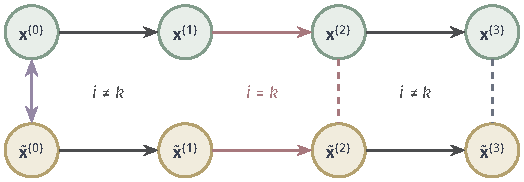
\includegraphics[width=88.74mm]{figures/05-optimization/05-stochastic-optimization/tikz/sgdb-coupling/figure.pdf}
  \caption{两次耦合运行。两条轨迹起点相同（紫色）。下标$i\neq k$时，两边用同一项更新，只传播已有差异；$i=k$时（红色箭头），两边用不同的项更新，新差异在此注入。}
  \label{fig:sgdb-coupling}
\end{BookInlineFigure}

\paragraph{用贯穿例计算}
取贯穿例，把第$3$项$f_3=\frac32(x-3)^2$换成$\tilde f_3=\frac32x^2$，也就是$b_3$从$3$变成$0$。起点都是$2$，$\alpha=0.1$，读取顺序为第$3,1,2$项，其中第一轮抽到被替换的项。两条轨迹依次是
\[
 \begin{aligned}
 x^{(1)}&=2.3, & \tilde x^{(1)}&=1.4, & \lvert x-\tilde x\rvert&=0.9,\\
 x^{(2)}&=1.77, & \tilde x^{(2)}&=0.96, & \lvert x-\tilde x\rvert&=0.81,\\
 x^{(3)}&=1.416, & \tilde x^{(3)}&=0.768, & \lvert x-\tilde x\rvert&=0.648.
 \end{aligned}
\]

第一轮两边的读数分别是$-3$和$6$，注入的差异是$0.1\cdot9=0.9$。后两轮用相同的项，$a_i=1,2$，差异分别乘以$1-\alpha a_i=0.9$和$0.8$，没有放大。下面的分析把这两种情形一般化。

\paragraph{传播：梯度步的非扩张}
先看未抽到被替换项的一步。两边用同一个函数走一步，距离不增加，这由下面的引理保证。这里为了证明简短，假定函数二阶连续可微。

\begin{lemma}[梯度步的非扩张与压缩]
\label{lem:sgdb-nonexpansive}
设$\phi$二阶连续可微，$\mu_0\bm{I}\preceq\nabla^2\phi\preceq L\bm{I}$，$\mu_0\geq0$。若$0<\alpha\leq2/(L+\mu_0)$，则对任意$\bm{x},\bm{y}$，
\begin{equation}
 \bigl\lVert\bigl(\bm{x}-\alpha\nabla\phi(\bm{x})\bigr)-\bigl(\bm{y}-\alpha\nabla\phi(\bm{y})\bigr)\bigr\rVert_2\leq(1-\alpha\mu_0)\lVert\bm{x}-\bm{y}\rVert_2 .
 \label{eq:sgdb-nonexpansive}
\end{equation}
\end{lemma}

\begin{proof}
由微积分基本定理，
\[
 \nabla\phi(\bm{x})-\nabla\phi(\bm{y})=\bm{A}(\bm{x}-\bm{y}),\qquad
 \bm{A}=\int_0^1\nabla^2\phi\bigl(\bm{y}+s(\bm{x}-\bm{y})\bigr)\,\mathrm{d}s .
\]

$\bm{A}$对称且$\mu_0\bm{I}\preceq\bm{A}\preceq L\bm{I}$。于是左端等于$\lVert(\bm{I}-\alpha\bm{A})(\bm{x}-\bm{y})\rVert_2$，矩阵$\bm{I}-\alpha\bm{A}$的特征值落在$[1-\alpha L,1-\alpha\mu_0]$内。条件$\alpha\leq2/(L+\mu_0)$保证$\alpha L-1\leq1-\alpha\mu_0$，所以这些特征值的绝对值不超过$1-\alpha\mu_0$，由此得到结论。
\end{proof}

\paragraph{注入与传播的合成}
差异只在抽到第$k$项时产生，每一步的概率是$1/N$。下面的定理把注入和传播合成一个界。

\begin{theorem}[样本替换下的期望参数距离]
\label{thm:sgdb-stability}
设每个$f_i$与$\tilde f_k$二阶连续可微，满足$\bm{0}\preceq\nabla^2\preceq L\bm{I}$。下标独立均匀抽取，确定的步长满足$0<\alpha^{(t)}\leq2/L$。设在两条轨迹访问的点上，被替换的两项梯度满足
\begin{equation}
 \lVert\nabla f_k(\bm{x}^{(t)})\rVert_2\leq G,\qquad \lVert\nabla\tilde f_k(\tilde{\bm x}^{(t)})\rVert_2\leq G .
 \label{eq:sgdb-stability-condition}
\end{equation}
则
\begin{equation}
 \mathbb{E}\lVert\bm{x}^{(T)}-\tilde{\bm x}^{(T)}\rVert_2\leq\frac{2G}{N}\sum_{t=0}^{T-1}\alpha^{(t)} .
 \label{eq:sgdb-stability}
\end{equation}
\end{theorem}

\begin{proof}
记两条轨迹的距离为
\[
 \delta^{(t)}=\lVert\bm{x}^{(t)}-\tilde{\bm x}^{(t)}\rVert_2,\qquad\delta^{(0)}=0.
\]

若$i^{(t)}\neq k$，两条轨迹用同一个$f_i$走一步，由引理~\ref{lem:sgdb-nonexpansive}（$\mu_0=0$），
\[
 \delta^{(t+1)}\leq\delta^{(t)} .
\]

若$i^{(t)}=k$，由三角不等式和式~\eqref{eq:sgdb-stability-condition}，
\[
 \delta^{(t+1)}\leq\delta^{(t)}+\alpha^{(t)}\bigl(\lVert\nabla f_k(\bm{x}^{(t)})\rVert_2+\lVert\nabla\tilde f_k(\tilde{\bm x}^{(t)})\rVert_2\bigr)\leq\delta^{(t)}+2\alpha^{(t)}G .
\]

下标与历史独立，后一种情形的条件概率是$1/N$，所以
\[
 \mathbb{E}\bigl[\delta^{(t+1)}\mid\mathcal{F}^{(t)}\bigr]\leq\delta^{(t)}+\frac{2\alpha^{(t)}G}{N}.
\]

取全期望，对$t=0,\ldots,T-1$累加，得到式~\eqref{eq:sgdb-stability}。
\end{proof}

这个界的结构是：每步以概率$1/N$注入不超过$2\alpha^{(t)}G$的差异，注入后的差异不再放大。若每项还$\mu_0$强凸，$\mu_0>0$，$\alpha\leq2/(L+\mu_0)$，引理给出的压缩因子就进入递推，常步长下
\[
 \mathbb{E}\delta^{(t+1)}\leq(1-\alpha\mu_0)\mathbb{E}\delta^{(t)}+\frac{2\alpha G}{N},
\]
它的极限不超过$2G/(N\mu_0)$，界不再随$T$无限增长。图~\ref{fig:sgdb-stability-run}(b)显示了实际平均距离与两条界：实际距离上升到约$0.04$后回落并稳定，远低于两条上界。上界偏保守的一个原因是$G$取了路径上的最大值，而实际注入的差异通常小于$2\alpha G$。

\begin{BookInlineFigure}
  \centering
  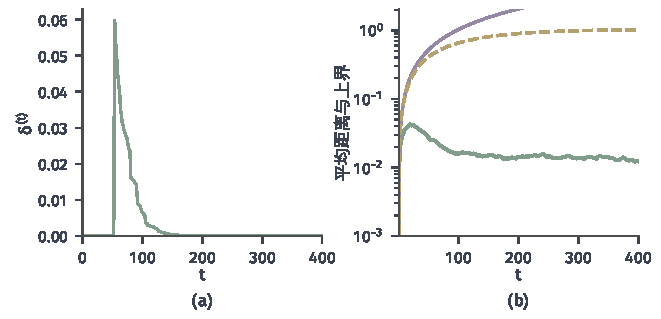
\includegraphics[width=112mm]{figures/05-optimization/05-stochastic-optimization/matplotlib/sgdb-stability-run/figure.pdf}
  \caption{样本替换的有限步响应，平方损失加平方惩罚的$N=100$项平均，$\gamma=0.2$，常步长$1/L_{\max}$，第$1$项被替换。(a)一条耦合路径上的距离$\delta^{(t)}$：抽到被替换项时跳起，之后逐渐压缩。(b)$1500$对路径的平均距离（绿），式~\eqref{eq:sgdb-stability}的非扩张界（紫）与利用强凸的压缩界（黄色虚线）。}
  \label{fig:sgdb-stability-run}
\end{BookInlineFigure}

\paragraph{结论的适用范围}
逐项的条件要逐一核对。这里要求的是每一项凸且光滑，只有平均目标凸是不够的，否则未抽到被替换项的那一步也可能拉开距离。凸性和步长决定传播：目标不凸时，梯度步可以把差异放大到$1+\alpha L$倍；步长超过$2/L$时，即使凸函数的梯度步也可能扩张。梯度界$G$只需要在实际访问的点上成立；对最小二乘这样的目标，它依赖轨迹所停留的区域。去掉二阶可微条件时，凸$L$光滑函数的梯度步仍然非扩张，证明需要梯度的余强制性，篇幅较长，读者可查阅\scite{hardt2016sgd}。

式~\eqref{eq:sgdb-stability}说的是参数的距离。要把它转成损失的变化，还需要损失对参数的定量控制：若损失关于参数$K$-Lipschitz，则损失之差不超过$K\lVert\bm{x}^{(T)}-\tilde{\bm x}^{(T)}\rVert_2$。这是另一个独立的条件。从算法的输出差异到统计泛化结论，还要有样本分布和数据生成假设，这部分不在有限步优化的范围内。

\section{本章小结}
\label{sec:sgd-summary}

本章回答了一个问题：不读全部目标项时，怎样构造更新并判断它的结果。抽样决定读取哪些项，读数的条件无偏是一切分析的起点，但单步读数可能指向上升方向，要靠期望递推和步长控制来管理噪声。

方差控制决定怎样利用额外读取和记忆。小批量、非均匀抽样和控制变量都能减小读数的方差，代价是快照、梯度表或抽样分布的维护。方差减小并不等同于总计算减少，要按相同的目标和精度比较。

动量、自适应尺度和方向处理分别改变实际更新的不同环节。动量把历史读数合成方向，平滑噪声的同时带来滞后，它对当前梯度不是无偏的，常步长下的噪声残余由有效步长决定。Nesterov方法的读数对应前瞻点，确定性的加速不能直接继承，噪声在势函数中留下不随步数消失的项。Lion与Muon对动量做非线性变换，分别舍弃坐标和奇异方向的幅度，实际位移、原目标残差和矩阵运算成本要分开核对。

自适应方法用历史幅度决定尺度。AdaGrad累计平方而难以遗忘，RMSProp用指数平均，Adam再加上方向平均和零初始化修正，AMSGrad让分母单调，AdamW把收缩与统计分开，Adafactor和Shampoo处理矩阵参数的存储和方向关系。这些尺度通常依赖当前读数，每种保证都必须连同它的假设一起引用，单调性之类的代数性质不是收敛结论。

裁剪、近似和替代让实际方向偏离梯度。把读数分解为真梯度、条件偏差和噪声，就能看到噪声项随步长缩小，偏差项不随步长缩小，而上界中的残余不一定是实际的下限。替代方向不是原目标的导数，评价和停止都要回到实际的前向目标。

所有保证都对应一个具体的目标、一个返回点和一个计算单位。同一个问题按更新次数和按读取量计时，方法的排序可以不同。有限步优化误差、路径的长期收敛和样本造成的统计误差是三个不同的问题，本章处理的是第一个，只说明了另外两个与它的分工。样本替换的分析则把算法看作从数据到输出的映射，为后续讨论统计误差提供了一种输入。

随机梯度方法需要目标的梯度读数。若只能读到函数值，就要先由函数值构造方向，下一章研究这个问题。


\chapter{零阶随机优化}
\label{chap:zeroth-order-optimization}

设想调节一台仿真器的两个参数。把参数填进去，运行一次，仿真器吐出一个代价数字。它的内部是几十万行别人写的程序，没有人能告诉你代价对参数的导数，甚至不确定这个导数处处存在。此前各章每一步都要读梯度，这里没有梯度可读，能做的只是换一组参数再试一次。

这样的处境里，局部方向只能靠函数值的差别来构造。\term{零阶优化}（zeroth-order optimization）指只使用函数值的优化，“零阶”相对于用梯度的一阶和用Hessian的二阶而言。本章讨论其中用随机扰动构造方向的一类方法，称为\term{零阶随机优化}（zeroth-order stochastic optimization，ZOSO）。全章用同一个目标核对每一步：
\begin{equation}
 f(\bm{x})=\frac12\bigl(x_1^2+9x_2^2\bigr),\qquad
 \bm{x}^{(0)}=(9,1).
 \label{eq:zo-example}
\end{equation}
它的梯度是$\nabla f(\bm{x})=(x_1,9x_2)$，$L=9$，$\mu=1$，起点处$f=45$，$\nabla f=(9,9)$。这些量只用来检查算法，算法本身看不到表达式，只能读数。

第~\ref{sec:zo-feedback}节先说清一次查询返回什么，因为后面所有结论都依赖这个接口。第~\ref{sec:zo-finite-differences}节用差商逼近原目标的梯度，会遇到两个对手：扰动尺度太大时的截断误差，太小时被放大的读数噪声。第~\ref{sec:zo-smoothing}节换一种看法：不去逼近原梯度，而是把目标在邻域上平均一下，于是函数值能够给出这个平均目标梯度的无偏估计。

有了方向，第~\ref{sec:zo-method}节把它接进迭代，需要分清算法到底在优化哪个目标。第~\ref{sec:zo-error-cost}节按函数读数次数比较各种方法，并回答最后一个问题：在平滑目标上得到的结论，对原目标意味着什么。

\section{函数值反馈}
\label{sec:zo-feedback}

调节仿真器参数时，算法与仿真器之间到底交换什么信息？同样叫“只能读函数值”，读数是否带噪声、一轮能读几个位置、两次读数能否共用一次仿真，会让后面的误差结论相差几个量级。所以先把接口固定下来。

\paragraph{目标、查询点与读数}
我们要最小化$f(\bm{x})$，$\bm{x}\in\bm{C}\subseteq\mathbb{R}^n$。算法每次提交一个\term{查询点}（query point）$\bm{q}\in\mathbb{R}^n$，黑箱返回一个实数$y$，称为\term{读数}（reading）。查询点不一定等于当前迭代点，算法常常故意偏离当前点一点，再比较读数。

这里出现两种性质不同的随机性，如图~\ref{fig:zo-feedback}所示。第一种在算法内部：算法自己抽取偏离的方向，这是我们主动加入的。第二种在黑箱内部：同一个查询点运行两次，可能因为测量噪声或仿真种子不同而得到不同的读数，这是我们无法控制的。

\begin{BookInlineFigure}
  \centering
  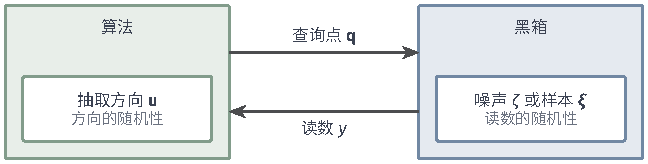
\includegraphics[width=110mm]{figures/05-optimization/05-stochastic-optimization/tikz/zo-feedback/figure.pdf}
  \caption{零阶优化的接口。算法提交查询点$\bm{q}$，黑箱返回读数$y$。方向$\bm{u}$的随机性由算法产生，噪声$\zeta$或样本$\bm{\xi}$的随机性来自黑箱，二者相互独立地起作用，分析时分别记录。}
  \label{fig:zo-feedback}
\end{BookInlineFigure}

\subsection{精确函数值与含噪读数}
\label{sec:zo-readings}

按黑箱内部的情况，读数分成三种模型。图~\ref{fig:zo-readings}画出了它们在一条一元曲线上的样子。

\paragraph{三种读数模型}
第一种是精确函数值，同一点读多少次都是同一个数：
\begin{equation}
 y=f(\bm{q}).
 \label{eq:zo-reading-exact}
\end{equation}
第二种是带\term{加性噪声}（additive noise）的读数，真实值上叠加一个随机误差$\zeta$：
\begin{equation}
 y=f(\bm{q})+\zeta.
 \label{eq:zo-reading-additive}
\end{equation}
第三种是期望目标的样本函数值。目标本身定义成随机函数的平均，一次读数对应一个随机场景$\bm{\xi}$：
\begin{equation}
 f(\bm{x})=\mathbb{E}_{\bm{\xi}}\bigl[F(\bm{x};\bm{\xi})\bigr],\qquad
 y=F(\bm{q};\bm{\xi}).
 \label{eq:zo-reading-sample}
\end{equation}

后两种的差别在于噪声是否依赖位置。贯穿例上取样本函数$F(\bm{x};\bm{\xi})=f(\bm{x})+\bm{\xi}^\top\bm{x}$，$\bm{\xi}$均值为零。场景$\bm{\xi}=(0.2,-0.1)$在起点给出
\[
 F(\bm{x}^{(0)};\bm{\xi})=45+0.2\cdot9-0.1\cdot1=46.7.
\]
这里偏差$1.7$随$\bm{x}$线性变化。固定一个场景，$F(\cdot;\bm{\xi})$是一条完整的曲线，如图~\ref{fig:zo-readings}(c)；而加性噪声模型里每次读数的误差是孤立的一个数，没有“这条曲线”可言。

\begin{BookInlineFigure}
  \centering
  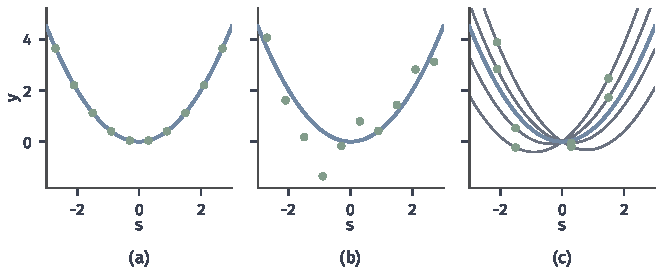
\includegraphics[width=112mm]{figures/05-optimization/05-stochastic-optimization/matplotlib/zo-readings/figure.pdf}
  \caption{同一个目标$s^2/2$（蓝线）的三种读数，绿点是读数。(a)精确读数落在曲线上。(b)加性噪声读数在曲线上下散开，标准差$0.6$。(c)样本函数$s^2/2+\xi s$，取四个场景$\xi$（灰线），绿点是同一场景曲线上的读数，蓝线是它们的期望。}
  \label{fig:zo-readings}
\end{BookInlineFigure}

\paragraph{无偏须对给定的历史和查询点成立}
什么叫“读数没有系统偏差”？直观要求是平均起来等于真值。但这个平均必须在“算法已经知道的一切”都固定时计算，否则算法可能恰好挑中噪声偏低的位置。记$\mathcal{H}$为提交本次查询之前算法产生的全部方向和读数。

\begin{definition}[条件无偏读数]
\label{def:zo-unbiased-reading}
读数$y$在查询点$\bm{q}$处称为\term{条件无偏}（conditionally unbiased）的，如果
\begin{equation}
 \mathbb{E}\bigl[y\mid\mathcal{H},\bm{q}\bigr]=f(\bm{q}).
 \label{eq:zo-conditional-unbiased}
\end{equation}
其方差有界是指：给定$\mathcal{H}$和$\bm{q}$时，$y$的条件方差不超过某个常数$\sigma^2<\infty$。
\end{definition}

条件期望可以理解为：把算法手里的信息看作已知常数，只对尚未发生的随机性求平均。严格定义可参考\BookChapterRef{chap:conditional-expectation}{卷七第4章“条件期望与条件分布”}，本章只用这一层含义和逐层取期望的规则。

边际无偏是不够的。设两个候选的真实值都是$0$，噪声等可能取$\pm1$，每个候选的噪声一旦生成就不再变化。先各读一次，然后挑读数较低的候选再读一次。第一次读数的边际均值是$0$，第二次读数却满足：
\[
 \mathbb{P}(\text{第二次读数}=-1)=\frac34,\qquad
 \mathbb{P}(\text{第二次读数}=+1)=\frac14.
\]
第二次读数的均值是$-\tfrac12$，而被选中候选的真值是$0$。噪声与“查询哪里”发生了关联，式~\eqref{eq:zo-conditional-unbiased}不成立。这说明重复使用同一份噪声时，查询点不能依赖这份噪声生成的读数。

\paragraph{目标确定时也可以用随机方向}
“随机优化”容易让人以为目标必须是随机的，其实不然。贯穿例~\eqref{eq:zo-example}若采用模型~\eqref{eq:zo-reading-exact}，黑箱完全确定。算法仍可以抽方向$\bm{u}=(0.6,0.8)$，查询$\bm{x}^{(0)}\pm0.5\bm{u}$，得到
\[
 f(9.3,1.4)=52.065,\qquad f(8.7,0.6)=39.465.
\]
重读多少次这两个数都不变，唯一的随机性是方向。反过来，若固定方向沿坐标轴逐个差分而读数带噪声，随机性就全部来自黑箱。两种随机性可以单独出现，也可以同时出现，分析时分开记录。

\subsection{单点查询与成对查询}
\label{sec:zo-pair-interface}

读数的模型说的是一次读数的性质，还需要规定多次读数之间的关系。这里有两个相互独立的问题。

\paragraph{一轮能读几个位置}
有些系统每次只能在一组参数下运行，下一轮参数已经变了，同一状态无法读第二个位置。这称为\term{单点查询}（single-point query）。另一些系统允许在同一轮提交两个位置，比如对称地偏离当前点，这称为\term{成对查询}（paired query）。前者更受限，后者能够比较两个读数，这是一项实质性的额外能力，不是实现细节。

\paragraph{两个位置能否共用一次仿真}
成对查询时还要问：两次读数用的是不是同一个随机场景？比如仿真器允许固定随机种子，那么可以读
\begin{equation}
 y_+=F(\bm{q}_+;\bm{\xi}),\qquad y_-=F(\bm{q}_-;\bm{\xi}),
 \label{eq:zo-shared-pair}
\end{equation}
也就是沿同一条样本曲线读两点。这称为\term{共享样本}（shared sample），又叫共同随机数。如果种子无法控制，两个读数各带独立的噪声：
\begin{equation}
 y_+=f(\bm{q}_+)+\zeta_+,\qquad y_-=f(\bm{q}_-)+\zeta_-.
 \label{eq:zo-independent-pair}
\end{equation}

\paragraph{为什么不能混为一谈}
两个模型的读数单独看可能分布完全相同，算差却完全不同。图~\ref{fig:zo-pair-readings}取$f(s)=s^2/2$，在$s=1$两侧相距$0.4$读两点，真实导数是$1$。左边噪声独立，分别取$+0.3$和$-0.3$，差商是
\[
 \frac{y_+-y_-}{2\cdot0.4}=\frac{(0.98+0.3)-(0.18-0.3)}{0.8}=1.75.
\]
右边两点共享噪声$+0.3$，差商里这个数被减掉，得到准确的$1$。相同大小的噪声，一边造成$75\%$的误差，一边没有影响。

\begin{BookInlineFigure}
  \centering
  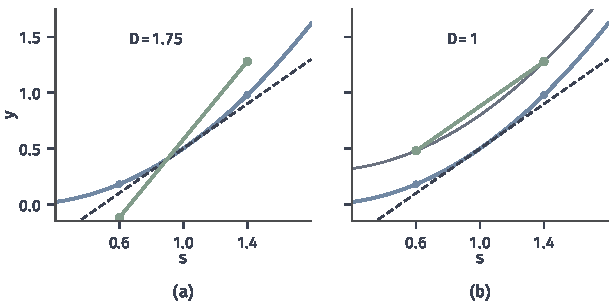
\includegraphics[width=104mm]{figures/05-optimization/05-stochastic-optimization/matplotlib/zo-pair-readings/figure.pdf}
  \caption{成对读数的两种接口，蓝线为$f(s)=s^2/2$，虚线是$s=1$处的切线，绿色线段连接两次读数，蓝点是真实函数值。(a)两点噪声独立，分别为$+0.3$和$-0.3$，线段斜率$1.75$，偏离切线。(b)两点共享噪声$+0.3$，读数都落在灰色曲线上，斜率恰为$1$。}
  \label{fig:zo-pair-readings}
\end{BookInlineFigure}

所以误差界必须与实际接口匹配。文献和本章后面给出的速率都带着接口条件，表~\ref{tab:zo-interfaces}先列出本章要用到的四种情形，第~\ref{sec:zo-pair-noise}节再推导对应的方差。

\begin{BookInlineTable}
  \centering
  \begin{tabular}{@{}lll@{}}
    \toprule
    接口 & 一轮读数 & 两点之差的噪声\\
    \midrule
    精确函数值 & 任意 & 无\\
    单点，含噪 & $1$ & 不适用\\
    成对，独立噪声 & $2$ & 方差$2\sigma^2$，不随距离变小\\
    成对，共享样本 & $2$ & 取决于样本函数的波动\\
    \bottomrule
  \end{tabular}
  \caption{本章区分的查询接口。“独立噪声”指式~\eqref{eq:zo-independent-pair}，噪声方差为$\sigma^2$；“共享样本”指式~\eqref{eq:zo-shared-pair}。}
  \label{tab:zo-interfaces}
\end{BookInlineTable}

\section{有限差分}
\label{sec:zo-finite-differences}

只凭几个函数值，怎样得到梯度的近似？思路来自一元微积分：导数是割线斜率的极限，步子小一点，割线斜率就接近导数。

\paragraph{从一元差商开始}
设$\varphi(s)$是一元函数，$h>0$是\term{扰动尺度}（perturbation scale）。两种常用的\term{差商}（difference quotient）是\term{前向差分}（forward difference）和\term{中心差分}（central difference）：
\begin{equation}
 \frac{\varphi(s+h)-\varphi(s)}{h},\qquad
 \frac{\varphi(s+h)-\varphi(s-h)}{2h}.
 \label{eq:zo-quotients-1d}
\end{equation}
图~\ref{fig:zo-secants}用$\varphi(s)=s^2/2+s^3/6$，$s_0=1$，$h=0.8$画出两条割线和切线。切线斜率是$\varphi'(1)=1.5$。

由$\varphi(1)=2/3$、$\varphi(1.8)=2.592$和$\varphi(0.2)\approx0.0213$，两种差商是
\[
 \frac{2.592-0.6667}{0.8}\approx2.407,\qquad
 \frac{2.592-0.0213}{1.6}\approx1.607.
\]
前向差商偏离$0.907$，中心差商只偏离$0.107$。原因是Taylor展开的二次项：前向割线把弯曲全部算进了斜率，中心割线的两侧弯曲互相抵消。

\begin{BookInlineFigure}
  \centering
  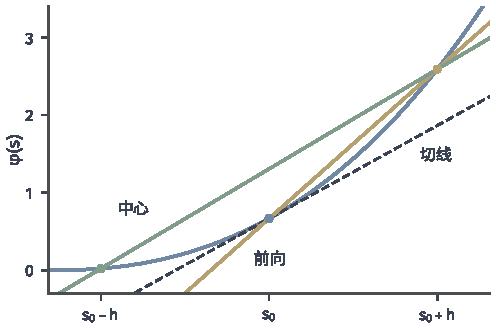
\includegraphics[width=84mm]{figures/05-optimization/05-stochastic-optimization/matplotlib/zo-secants/figure.pdf}
  \caption{$\varphi(s)=s^2/2+s^3/6$（蓝线）在$s_0=1$处的两种差商，$h=0.8$。虚线是切线，斜率$1.5$；黄线是前向割线，斜率约$2.407$；绿线是中心割线，斜率约$1.607$，方向最接近切线。}
  \label{fig:zo-secants}
\end{BookInlineFigure}

\paragraph{多元函数：沿一个方向看}
差商搬到多元函数上，只要限制在一条直线上。令$\varphi(s)=f(\bm{x}+s\bm{u})$，由链式法则$\varphi'(0)=\langle\nabla f(\bm{x}),\bm{u}\rangle$，这是方向导数。于是沿$\bm{u}$的中心差商近似$\langle\nabla f(\bm{x}),\bm{u}\rangle$。一次差商只告诉我们梯度在一个方向上的投影，要拼出整个梯度，需要多个方向，或者后面将看到的随机化。

下面的引理量化差商的\term{截断误差}（truncation error），它只涉及函数本身，不涉及噪声。第~\ref{chap:smooth-foundations}章的下降引理给出：$\nabla f$是$L$-Lipschitz时，对任意$\bm{x},\bm{v}$，
\[
 \bigl\lvert f(\bm{x}+\bm{v})-f(\bm{x})-\langle\nabla f(\bm{x}),\bm{v}\rangle\bigr\rvert
 \leq\frac{L}{2}\lVert\bm{v}\rVert_2^2.
\]

\begin{lemma}[差商的余项]
\label{lem:zo-remainder}
设$\nabla f$是$L$-Lipschitz的。对任意$\bm{x},\bm{v}$，
\begin{equation}
 \bigl\lvert f(\bm{x}+\bm{v})-f(\bm{x}-\bm{v})-2\langle\nabla f(\bm{x}),\bm{v}\rangle\bigr\rvert
 \leq L\lVert\bm{v}\rVert_2^2.
 \label{eq:zo-central-L}
\end{equation}
若$f$还二阶连续可微，且$\nabla^2f$按谱范数是$M$-Lipschitz的，则
\begin{equation}
 \bigl\lvert f(\bm{x}+\bm{v})-f(\bm{x}-\bm{v})-2\langle\nabla f(\bm{x}),\bm{v}\rangle\bigr\rvert
 \leq\frac{M}{3}\lVert\bm{v}\rVert_2^3.
 \label{eq:zo-central-M}
\end{equation}
\end{lemma}

\begin{proof}
把上面的不等式分别用于$\bm{v}$和$-\bm{v}$，两式相减，由三角不等式得式~\eqref{eq:zo-central-L}。

对第二个结论，记$\bm{H}=\nabla^2f(\bm{x})$。积分形式的Taylor公式给出
\[
 \begin{aligned}
 &f(\bm{x}+\bm{v})-f(\bm{x})-\langle\nabla f(\bm{x}),\bm{v}\rangle-\frac12\bm{v}^\top\bm{H}\bm{v}\\
 &\quad=\int_0^1(1-s)\,\bm{v}^\top\bigl(\nabla^2f(\bm{x}+s\bm{v})-\bm{H}\bigr)\bm{v}\,\mathrm{d}s.
 \end{aligned}
\]
右端的绝对值不超过
\[
 \int_0^1(1-s)\,Ms\,\lVert\bm{v}\rVert_2^3\,\mathrm{d}s=\frac{M}{6}\lVert\bm{v}\rVert_2^3.
\]
对$\bm{v}$和$-\bm{v}$各写一次再相减，二次项$\tfrac12\bm{v}^\top\bm{H}\bm{v}$恰好相消，余项相加得$\tfrac{M}{3}\lVert\bm{v}\rVert_2^3$。
\end{proof}

\paragraph{三笔账}
每种差分都要记三笔账。第一笔是截断误差，随$h$变小而变小。第二笔是读数噪声造成的误差：独立噪声方差$\sigma^2$时，前向差商的噪声是$(\zeta_1-\zeta_0)/h$，中心差商的噪声是$(\zeta_+-\zeta_-)/(2h)$，方差分别为
\begin{equation}
 \frac{2\sigma^2}{h^2},\qquad\frac{\sigma^2}{2h^2},
 \label{eq:zo-quotient-noise}
\end{equation}
都随$h$变小而变大。第三笔是查询次数。这三笔账彼此独立，下面逐个方法记录，第~\ref{sec:zo-tradeoff}节再做取舍。

\subsection{坐标差分}
\label{sec:zo-coordinate}

最直接的做法是沿$n$个坐标方向逐个差分，用$n$个方向导数拼成梯度。记$\bm{e}_i$为第$i$个标准基向量，两种\term{坐标差分}（coordinate difference）的第$i$个分量是
\begin{equation}
 \hat{g}^{\mathrm{F}}_i=\frac{f(\bm{x}+h\bm{e}_i)-f(\bm{x})}{h},\qquad
 \hat{g}^{\mathrm{C}}_i=\frac{f(\bm{x}+h\bm{e}_i)-f(\bm{x}-h\bm{e}_i)}{2h}.
 \label{eq:zo-coordinate}
\end{equation}

\paragraph{查询次数}
前向差分的$n$个分量可以共用中心读数$f(\bm{x})$，所以一共$n+1$次查询。中心差分每个坐标读两点，共$2n$次，中心点本身不读。图~\ref{fig:zo-stencils}(a)(b)画出了这两种查询模式。

\begin{BookInlineFigure}
  \centering
  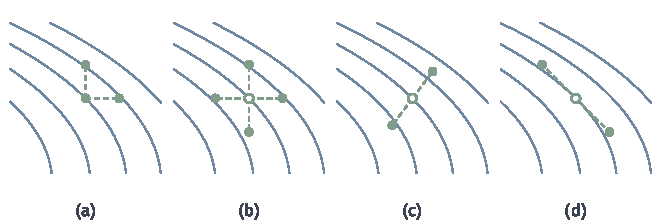
\includegraphics[width=112mm]{figures/05-optimization/05-stochastic-optimization/matplotlib/zo-stencils/figure.pdf}
  \caption{贯穿例在$(9,1)$附近的查询点，蓝线是等高线，为便于观察取$h=0.4$。实心点要读函数值，空心点是当前点、不读。(a)前向坐标差分，$3$次。(b)中心坐标差分，$4$次。(c)沿$\bm{u}=(0.6,0.8)$的随机方向差分，$2$次。(d)第~\ref{sec:zo-spsa}节的同时扰动，$\bm{\Delta}=(1,-1)$，$2$次，位移长度是$h\sqrt{2}$。}
  \label{fig:zo-stencils}
\end{BookInlineFigure}

\paragraph{手算比较}
在贯穿例的起点取$h=0.1$。为算前向差商，读三个函数值：
\[
 f(9,1)=45,\qquad f(9.1,1)=45.905,\qquad f(9,1.1)=45.945.
\]
代入式~\eqref{eq:zo-coordinate}，前向差分给出
\[
 \hat{\bm{g}}^{\mathrm{F}}=(9.05,\ 9.45).
\]
真实梯度是$(9,9)$，误差$(0.05,\,0.45)$，恰好等于$\tfrac{h}{2}H_{ii}$：沿$x_2$方向弯曲是$x_1$方向的$9$倍，误差也是$9$倍。

再读$f(8.9,1)=44.105$和$f(9,0.9)=44.145$，中心差分给出
\[
 \hat{\bm{g}}^{\mathrm{C}}=\Bigl(\frac{45.905-44.105}{0.2},\ \frac{45.945-44.145}{0.2}\Bigr)=(9,\ 9).
\]
对二次函数，中心差分没有截断误差，因为三阶以上的导数都是零。多付一次查询，换来了精确值。

\paragraph{截断误差的一般结论}
上面的现象对一般函数也成立，只是阶数要由相应的导数条件来保证。

\begin{theorem}[坐标差分的截断误差]
\label{thm:zo-coordinate}
设读数精确。若$\nabla f$是$L$-Lipschitz的，则
\begin{equation}
 \lVert\hat{\bm{g}}^{\mathrm{F}}-\nabla f(\bm{x})\rVert_2\leq\frac{\sqrt{n}\,Lh}{2}.
 \label{eq:zo-coordinate-forward}
\end{equation}
若$f$还二阶连续可微且$\nabla^2f$是$M$-Lipschitz的，则
\begin{equation}
 \lVert\hat{\bm{g}}^{\mathrm{C}}-\nabla f(\bm{x})\rVert_2\leq\frac{\sqrt{n}\,Mh^2}{6}.
 \label{eq:zo-coordinate-central}
\end{equation}
\end{theorem}

\begin{proof}
对前向差分，把下降引理用于$\bm{v}=h\bm{e}_i$，再除以$h$，得
\[
 \lvert\hat{g}^{\mathrm{F}}_i-\partial_if(\bm{x})\rvert\leq\frac{Lh}{2}.
\]

对中心差分，把式~\eqref{eq:zo-central-M}用于$\bm{v}=h\bm{e}_i$，再除以$2h$，得
\[
 \lvert\hat{g}^{\mathrm{C}}_i-\partial_if(\bm{x})\rvert\leq\frac{Mh^2}{6}.
\]
$n$个分量各不超过同一个上界，向量的欧氏范数不超过该上界乘以$\sqrt{n}$。
\end{proof}

定理的条件各有作用。前向差分只用到梯度的Lipschitz性，误差是一阶的。中心差分要快一阶，需要三阶信息受控，也就是Hessian的Lipschitz性；只有$L$时，由式~\eqref{eq:zo-central-L}只能得到每个分量$Lh/2$，与前向差分同阶。

图~\ref{fig:zo-trunc-log}在$\varphi(s)=s^2/2+s^3/6$上验证这两个阶数。双对数坐标下，前向误差的斜率是$1$，中心误差的斜率是$2$，$h$每缩小$10$倍，中心差分的误差缩小$100$倍。

\begin{BookInlineFigure}
  \centering
  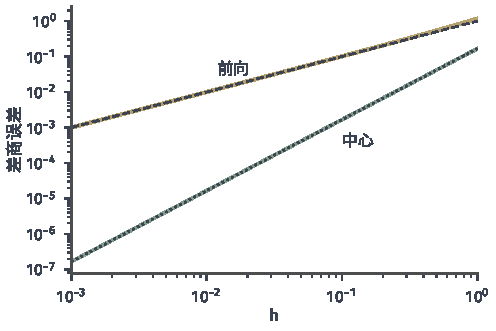
\includegraphics[width=84mm]{figures/05-optimization/05-stochastic-optimization/matplotlib/zo-trunc-log/figure.pdf}
  \caption{精确读数下差商误差随$h$的变化，$\varphi(s)=s^2/2+s^3/6$，$s_0=1$，真实导数$1.5$。黄线为前向差分，绿线为中心差分；虚线是$h$，点线是$h^2/6$，分别对应理论的斜率$1$和$2$。}
  \label{fig:zo-trunc-log}
\end{BookInlineFigure}

\subsection{随机方向差分}
\label{sec:zo-random-direction}

坐标差分每算一次梯度要$n$轮查询，维数大时一步也走不起。一个自然的想法是：每轮只沿一个方向差分，方向随机抽，多轮平均下来也许能覆盖各个方向。

\paragraph{从方向导数恢复向量}
一次差商是一个标量，要把它变成向量，乘上方向本身。设$\bm{u}$在单位球面$\bm{S}$（$\mathbb{R}^n$中全体长度为$1$的向量）上均匀分布。记$\bm{g}=\nabla f(\bm{x})$，考察$\langle\bm{g},\bm{u}\rangle\bm{u}$的均值。由对称性，$\mathbb{E}[u_iu_j]=0$（$i\neq j$），且$n$个$\mathbb{E}[u_i^2]$相等，和为$1$，所以
\[
 \mathbb{E}[\bm{u}\bm{u}^\top]=\frac{1}{n}\bm{I}.
\]
于是
\[
 \mathbb{E}\bigl[\langle\bm{g},\bm{u}\rangle\bm{u}\bigr]=\mathbb{E}[\bm{u}\bm{u}^\top]\bm{g}=\frac{1}{n}\bm{g}.
\]
乘以$n$就得到$\bm{g}$的无偏量。把方向导数换成中心差商，定义\term{随机方向差分}（random-direction difference）：
\begin{equation}
 D_h(\bm{u})=\frac{f(\bm{x}+h\bm{u})-f(\bm{x}-h\bm{u})}{2h},\qquad
 \hat{\bm{g}}=n\,D_h(\bm{u})\,\bm{u}.
 \label{eq:zo-random-direction}
\end{equation}
一般地，若方向分布满足$\mathbb{E}[\bm{u}\bm{u}^\top]=c\,\bm{I}$，归一化因子就是$1/c$。因子$n$来自单位球面的二阶矩，不是万能常数。

\paragraph{一条方向只有一条方向的信息}
在起点，贯穿例是二次函数，中心差商精确等于方向导数，$\hat{\bm{g}}=2\langle\bm{g},\bm{u}\rangle\bm{u}$。取几个方向，结果如下：
\[
 \bm{u}=(1,0):\ \hat{\bm{g}}=(18,0),\qquad
 \bm{u}=(0,1):\ \hat{\bm{g}}=(0,18).
\]
第三、第四个方向是$(1,1)/\sqrt{2}$和$(1,-1)/\sqrt{2}$，得到
\[
 \hat{\bm{g}}=(18,18),\qquad\hat{\bm{g}}=(0,0).
\]
四个估计的平均是$(9,9)$，但没有一个单独接近$(9,9)$。方向$(1,-1)/\sqrt{2}$与梯度垂直，一条差商得到零，什么也看不出来。

图~\ref{fig:zo-circle}(a)说明所有估计的分布：$n=2$时，$2\langle\bm{g},\bm{u}\rangle\bm{u}$走遍一个以$\bm{g}$为圆心、过原点的圆。圆心就是均值，半径就是误差的大小。单个估计总是偏离$\lVert\bm{g}\rVert_2$，只有平均才接近$\bm{g}$。

\begin{BookInlineFigure}
  \centering
  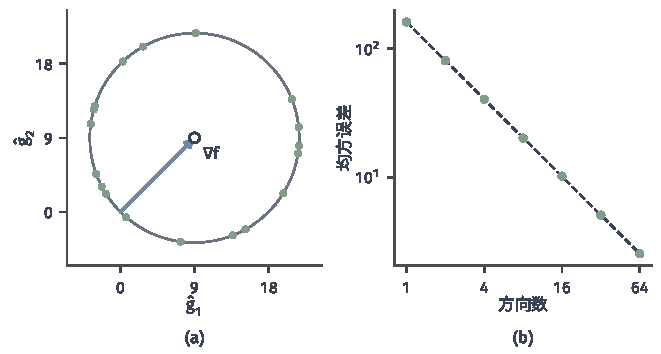
\includegraphics[width=112mm]{figures/05-optimization/05-stochastic-optimization/matplotlib/zo-circle/figure.pdf}
  \caption{贯穿例起点处$\bm{g}=(9,9)$的随机方向估计。(a)绿点是$18$个随机方向给出的$2\langle\bm{g},\bm{u}\rangle\bm{u}$，全部落在以$\bm{g}$（空心圆）为圆心、半径$\lVert\bm{g}\rVert_2$的灰圆上，蓝色箭头是真实梯度。(b)$m$个独立方向平均后的均方误差，绿点是Monte Carlo结果，虚线是$162/m$。}
  \label{fig:zo-circle}
\end{BookInlineFigure}

\paragraph{偏差与二阶矩}
下面的定理把偏差和波动分开。

\begin{theorem}[随机方向差分]
\label{thm:zo-random-direction}
设读数精确，$\bm{u}$在$\bm{S}$上均匀分布，$\hat{\bm{g}}$由式~\eqref{eq:zo-random-direction}定义。若$f$是二次函数，则
\begin{equation}
 \mathbb{E}[\hat{\bm{g}}]=\bm{g},\qquad
 \mathbb{E}\lVert\hat{\bm{g}}-\bm{g}\rVert_2^2=(n-1)\lVert\bm{g}\rVert_2^2.
 \label{eq:zo-direction-quadratic}
\end{equation}
若$f$二阶连续可微且$\nabla^2f$是$M$-Lipschitz的，则偏差满足
\begin{equation}
 \bigl\lVert\mathbb{E}[\hat{\bm{g}}]-\bm{g}\bigr\rVert_2\leq\frac{nMh^2}{6}.
 \label{eq:zo-direction-bias}
\end{equation}
\end{theorem}

\begin{proof}
二次函数的中心差商没有余项，$\hat{\bm{g}}=n\langle\bm{g},\bm{u}\rangle\bm{u}$，由$\mathbb{E}[\bm{u}\bm{u}^\top]=\bm{I}/n$得$\mathbb{E}[\hat{\bm{g}}]=\bm{g}$。

二阶矩用$\lVert\bm{u}\rVert_2=1$计算：
\[
 \mathbb{E}\lVert\hat{\bm{g}}\rVert_2^2=n^2\mathbb{E}\langle\bm{g},\bm{u}\rangle^2=n^2\cdot\frac{\lVert\bm{g}\rVert_2^2}{n}=n\lVert\bm{g}\rVert_2^2.
\]
减去均值的平方$\lVert\bm{g}\rVert_2^2$，得到方差。

一般情形写$D_h(\bm{u})=\langle\bm{g},\bm{u}\rangle+r$。把式~\eqref{eq:zo-central-M}用于$\bm{v}=h\bm{u}$并除以$2h$，得$\lvert r\rvert\leq Mh^2/6$。于是
\[
 \bigl\lVert\mathbb{E}[\hat{\bm{g}}]-\bm{g}\bigr\rVert_2=n\bigl\lVert\mathbb{E}[r\bm{u}]\bigr\rVert_2\leq n\,\mathbb{E}\lvert r\rvert\leq\frac{nMh^2}{6}.
\]
\end{proof}

式~\eqref{eq:zo-direction-quadratic}的$n-1$就是维数的代价：一条方向只探测了$n$维中的一维，其余$n-1$维的信息要靠多轮平均。图~\ref{fig:zo-circle}(b)验证了$m$个独立方向平均后，均方误差按$(n-1)\lVert\bm{g}\rVert_2^2/m$下降。

\paragraph{有限扰动下一般有偏}
二次函数上的无偏是特例。一旦有三阶项，中心差商不再等于方向导数，由它乘$\bm{u}$形成的向量，均值一般不等于原梯度。取$n=2$，$f(\bm{x})=x_1^3$，在$x_1=0$处真实梯度为零。差商和估计为
\[
 D_h(\bm{u})=h^2u_1^3,\qquad\hat{\bm{g}}=2h^2u_1^3\,\bm{u}.
\]
记$\bm{u}=(\cos\theta,\sin\theta)$。由$\mathbb{E}[\cos^4\theta]=\tfrac38$和$\mathbb{E}[\cos^3\theta\sin\theta]=0$，
\[
 \mathbb{E}[\hat{\bm{g}}]=\bigl(\tfrac34h^2,\ 0\bigr)\neq\bm{0}.
\]
这里$M=6$，定理的界是$2h^2$，实际偏差$\tfrac34h^2$在界内。偏差确实存在，而且随$h$平方缩小。

\subsection{同时扰动随机逼近}
\label{sec:zo-spsa}

随机方向差分要从球面上抽方向，并且需要因子$n$。Spall提出的\term{同时扰动随机逼近}（simultaneous perturbation stochastic approximation，SPSA）用更简单的方式达到类似的效果：让所有坐标同时动一下，每个坐标只取正负两个方向。

\paragraph{主要思想}
抽取向量$\bm{\Delta}\in\{-1,+1\}^n$，各分量独立，等可能取$\pm1$。查询两点$\bm{x}\pm h\bm{\Delta}$，算一个函数差，再把同一个差除以各分量的扰动：
\begin{equation}
 D=\frac{y_+-y_-}{2h},\qquad \hat{g}_i=\frac{D}{\Delta_i},\quad i=1,\ldots,n.
 \label{eq:zo-spsa}
\end{equation}
只读了两次，却得到了$n$个分量。为什么这样能行？若$f$是二次函数，$D=\langle\bm{g},\bm{\Delta}\rangle$，于是
\[
 \hat{g}_i=g_i+\sum_{j\neq i}g_j\frac{\Delta_j}{\Delta_i}.
\]
第一项是想要的。后面每一项都是其他坐标的“串扰”。因为$\Delta_j$与$\Delta_i$独立，且$\mathbb{E}[\Delta_j]=0$，串扰的均值是零，平均之后消失。

除法要求$\mathbb{E}[1/\lvert\Delta_i\rvert]$有限，这解释了分布的选择。正态或区间上的均匀扰动在$0$附近有正的密度，$1/\lvert\Delta_i\rvert$的期望发散，不能用于这个公式。$\pm1$时$1/\Delta_i=\Delta_i$，估计也可以写成$\hat{\bm{g}}=D\,\bm{\Delta}$。

\paragraph{手算四种情形}
贯穿例起点，$h=0.1$，$n=2$，$\bm{\Delta}$有四种等可能取值。取$\bm{\Delta}=(1,1)$，读数和差商是
\[
 y_+=f(9.1,1.1)=46.85,\qquad y_-=f(8.9,0.9)=43.25,\qquad D=18.
\]
取$\bm{\Delta}=(1,-1)$，两次读数相等，差商为零：
\[
 y_+=f(9.1,0.9)=45.05,\qquad y_-=f(8.9,1.1)=45.05,\qquad D=0.
\]
$-\bm{\Delta}$与$\bm{\Delta}$的结果相同。四种情形的估计分别是$(18,18)$、$(0,0)$、$(0,0)$、$(18,18)$，平均恰为$(9,9)$，如图~\ref{fig:zo-spsa}(b)。

\begin{BookInlineFigure}
  \centering
  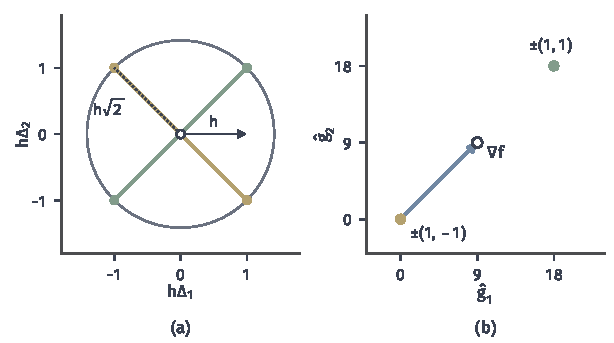
\includegraphics[width=104mm]{figures/05-optimization/05-stochastic-optimization/matplotlib/zo-spsa/figure.pdf}
  \caption{$n=2$时的同时扰动。(a)四个扰动$h\bm{\Delta}$（$h=1$）位于正方形顶点，一对相反的点共用一次差分，绿、黄各一对；每个坐标只动$h$，位移长度却是$h\sqrt{2}$，四点都在半径$h\sqrt{2}$的圆上。(b)贯穿例起点的估计，绿点是$\bm{\Delta}=\pm(1,1)$的结果，黄点是$\bm{\Delta}=\pm(1,-1)$的结果，它们的平均是真实梯度（空心圆）。}
  \label{fig:zo-spsa}
\end{BookInlineFigure}

\paragraph{偏差与噪声}
SPSA在原梯度上的偏差由差商余项决定，与随机方向差分的结论形式一样，只是这里的位移长度不再是$h$。

\begin{theorem}[SPSA的偏差]
\label{thm:zo-spsa}
设$f$二阶连续可微，$\nabla^2f$是$M$-Lipschitz的，$\bm{\Delta}$的分量独立且等可能取$\pm1$，读数为$y_\pm=f(\bm{x}\pm h\bm{\Delta})+\zeta_\pm$，且给定$\bm{x},\bm{\Delta}$时$\zeta_+-\zeta_-$的条件均值为零。则对$\hat{\bm{g}}$的每个分量，
\begin{equation}
 \bigl\lvert\mathbb{E}[\hat{g}_i\mid\bm{x}]-\partial_if(\bm{x})\bigr\rvert\leq\frac{M h^2n^{3/2}}{6}.
 \label{eq:zo-spsa-bias}
\end{equation}
\end{theorem}

\begin{proof}
$\lVert h\bm{\Delta}\rVert_2=h\sqrt{n}$。把差商写成主项、余项和噪声三部分：
\[
 D=\langle\bm{g},\bm{\Delta}\rangle+r+\frac{\zeta_+-\zeta_-}{2h}.
\]
由式~\eqref{eq:zo-central-M}，余项满足
\[
 \lvert r\rvert\leq\frac{1}{2h}\cdot\frac{M}{3}(h\sqrt{n})^3=\frac{Mh^2n^{3/2}}{6}.
\]
除以$\Delta_i$后取条件期望。主项由串扰的零均值给出$g_i$；噪声项先对给定的$\bm{\Delta}$取期望，为零；余项的绝对值不变，因为$\lvert\Delta_i\rvert=1$。
\end{proof}

对二次函数$r=0$，SPSA精确无偏。一般函数上$h$有限时仍有偏差，只有$h\to0$时偏差才消失，这一点与随机方向差分相同。定理只要求噪声差的条件均值为零，噪声本身不必独立。

\paragraph{坐标尺度与位移长度}
比较SPSA和球面方向时容易犯一个错误：SPSA的$h$是每个坐标的扰动，实际位移长度是$h\sqrt{n}$。在$n=100$、$h=0.1$时，查询点已偏离当前点$1$个单位。公平的比较要令位移长度相同，取$h=\delta/\sqrt{n}$与球面半径$\delta$对应。

这样比较之后两者的噪声完全一致。独立噪声下，SPSA的$\lVert\hat{\bm{g}}\rVert_2^2$中噪声贡献的均值是$n\sigma^2/(2h^2)$，代入$h=\delta/\sqrt{n}$得
\[
 \frac{n^2\sigma^2}{2\delta^2},
\]
恰好等于球面方向的噪声贡献$n^2\cdot\sigma^2/(2\delta^2)$。二次函数上，SPSA的二阶矩也与球面方向相同：
\[
 \mathbb{E}\lVert\hat{\bm{g}}\rVert_2^2=n\,\mathbb{E}\langle\bm{g},\bm{\Delta}\rangle^2=n\lVert\bm{g}\rVert_2^2.
\]
SPSA的优势主要在实现简单，每个坐标扰动大小固定。

表~\ref{tab:zo-differences}汇总本节三种差分。

\begin{BookInlineTable}
  \centering
  \begin{tabular}{@{}llll@{}}
    \toprule
    方法 & 查询 & 截断偏差 & 独立噪声的二阶矩\\
    \midrule
    前向坐标 & $n+1$ & $\sqrt{n}Lh/2$ & $2n\sigma^2/h^2$\\
    中心坐标 & $2n$ & $\sqrt{n}Mh^2/6$ & $n\sigma^2/(2h^2)$\\
    随机方向 & $2$ & $nMh^2/6$ & $n^2\sigma^2/(2h^2)$\\
    SPSA & $2$ & $n^2Mh^2/6$ & $n\sigma^2/(2h^2)$\\
    \bottomrule
  \end{tabular}
  \caption{三种差分的成本与误差。偏差为欧氏范数的上界，SPSA一行由式~\eqref{eq:zo-spsa-bias}乘$\sqrt{n}$得到。独立噪声的二阶矩指$\mathbb{E}\lVert\text{噪声造成的估计误差}\rVert_2^2$，SPSA的$h$是坐标尺度，位移长度为$h\sqrt{n}$。}
  \label{tab:zo-differences}
\end{BookInlineTable}

\section{随机平滑与梯度估计}
\label{sec:zo-smoothing}

上一节的估计以原梯度为目标，有限的$h$总带来偏差。于是要问：能否换一个目标，让函数值给出的估计严格无偏？答案是把目标函数在一个小邻域上取平均。平均之后的函数有自己的梯度，而这个梯度恰好可以写成函数值的期望。

打个比方，用原目标比较两点的高低，好比踩着一块小石头判断地面坡度，容易被局部起伏误导；平滑目标则像站在一块平板上，平板的倾斜由它覆盖的整片地面决定。我们估计的是平板的倾斜，不是脚下那一点的坡度。比方的边界也要记住：平板的倾斜和地面的坡度是两个对象，它们的差别要到第~\ref{sec:zo-original-error}节才算清。

\subsection{平滑目标}
\label{sec:zo-smooth-target}

\paragraph{定义}
记$\bm{B}$为$\mathbb{R}^n$中的单位球，即全体长度不超过$1$的向量。下面给出两种平均方式，$\delta>0$是球的半径，$\tau>0$是高斯分布的尺度。

\begin{definition}[球平滑与高斯平滑]
\label{def:zo-smoothing}
设$\bm{v}$在$\bm{B}$上均匀分布，$\bm{w}\sim\mathcal{N}(\bm{0},\bm{I})$。$f$的\term{球平滑}（ball smoothing）与\term{高斯平滑}（Gaussian smoothing）分别是
\begin{equation}
 f^{\mathrm{B}}_{\delta}(\bm{x})=\mathbb{E}_{\bm{v}}\bigl[f(\bm{x}+\delta\bm{v})\bigr],\qquad
 f^{\mathrm{G}}_{\tau}(\bm{x})=\mathbb{E}_{\bm{w}}\bigl[f(\bm{x}+\tau\bm{w})\bigr].
 \label{eq:zo-smoothing}
\end{equation}
前提是期望有定义。它们统称\term{平滑目标}（smoothed objective）。
\end{definition}

\paragraph{定义成立需要什么}
两种平均对$f$的要求不同。球平滑只看$\bm{x}$周围半径$\delta$的球，$f$在这个球上局部可积就够了，比如局部连续。它对球外的$f$没有任何要求。

高斯平滑要看整个空间，于是必须控制$f$在无穷远的增长，局部的好性质帮不上忙。例如$n=1$，$f(x)=e^{x^2}$处处光滑，但
\[
 \mathbb{E}\bigl[e^{(x+\tau w)^2}\bigr]<\infty\quad\Longleftrightarrow\quad 2\tau^2<1.
\]
$\tau\geq1/\sqrt{2}$时高斯平滑根本不存在。多项式增长或指数增长（$\lvert f(\bm{z})\rvert$不超过$Ce^{a\lVert\bm{z}\rVert_2}$）都可以被高斯密度压住。

\paragraph{二次函数上的平滑}
贯穿例上平滑的效果可以算出来。二次函数满足
\[
 f(\bm{x}+\bm{z})=f(\bm{x})+\langle\nabla f(\bm{x}),\bm{z}\rangle+\frac12\bm{z}^\top\bm{H}\bm{z}.
\]
取$\bm{z}$为对称分布的扰动，一次项的期望为零。均匀球上$\mathbb{E}[\bm{v}\bm{v}^\top]=\bm{I}/(n+2)$，所以
\[
 f^{\mathrm{B}}_{\delta}(\bm{x})=f(\bm{x})+\frac{\delta^2\operatorname{tr}\bm{H}}{2(n+2)},\qquad
 f^{\mathrm{G}}_{\tau}(\bm{x})=f(\bm{x})+\frac{\tau^2\operatorname{tr}\bm{H}}{2}.
\]
贯穿例$\operatorname{tr}\bm{H}=10$，$n=2$，分别得到$f+1.25\delta^2$和$f+5\tau^2$。平滑只把目标抬高一个常数，梯度完全不变。所以在二次函数上，平滑目标的梯度就是原梯度，这也解释了上一节的中心差分为什么在二次函数上无偏。

\paragraph{绝对值函数：不可微时平滑仍可微}
平滑真正的用处在不光滑的目标上。$f(x)=\lvert x\rvert$在$0$处没有导数。$n=1$时单位球是区间$[-1,1]$，直接积分得到
\begin{equation}
 f^{\mathrm{B}}_{\delta}(x)=
 \begin{cases}
 \dfrac{x^2+\delta^2}{2\delta},&\lvert x\rvert\leq\delta,\\
 \lvert x\rvert,&\lvert x\rvert>\delta.
 \end{cases}
 \label{eq:zo-abs-ball}
\end{equation}
它的导数在$\lvert x\rvert\leq\delta$上是$x/\delta$，在$x=\pm\delta$处与外侧的$\pm1$衔接，因此连续可微。高斯平滑的结果用误差函数表示：
\[
 f^{\mathrm{G}}_{\tau}(x)=\tau\sqrt{\frac{2}{\pi}}\,e^{-x^2/(2\tau^2)}+x\operatorname{erf}\Bigl(\frac{x}{\sqrt{2}\tau}\Bigr).
\]
图~\ref{fig:zo-smooth-abs}取$\delta=1$，$\tau=1/\sqrt{3}$，这时两种扰动的方差相同。尖点被磨圆了，但代价也在图上：$x=0$处，两条曲线的值分别是$1/2$和约$0.46$，原函数值是$0$。

\begin{BookInlineFigure}
  \centering
  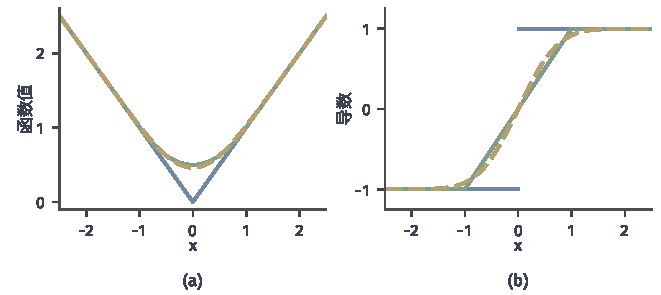
\includegraphics[width=112mm]{figures/05-optimization/05-stochastic-optimization/matplotlib/zo-smooth-abs/figure.pdf}
  \caption{$f(x)=\lvert x\rvert$的平滑。蓝线是原函数，绿线是$\delta=1$的球平滑，黄色虚线是$\tau=1/\sqrt{3}$的高斯平滑。(a)函数值，尖点被磨圆且抬高。(b)导数，原函数在$0$处跳变，平滑后连续。}
  \label{fig:zo-smooth-abs}
\end{BookInlineFigure}

\paragraph{平滑误差}
平滑目标与原目标差多少，由原目标的光滑程度决定。下面的引理后面会多次使用。

\begin{lemma}[平滑的基本性质]
\label{lem:zo-smoothing-properties}
\begin{enumerate}
 \item 若$\nabla f$是$L$-Lipschitz的，则$f^{\mathrm{B}}_{\delta}$与$f^{\mathrm{G}}_{\tau}$的梯度也是$L$-Lipschitz的，并且
 \begin{equation}
  \lvert f^{\mathrm{B}}_{\delta}-f\rvert\leq\frac{L\delta^2}{2},\qquad
  \lVert\nabla f^{\mathrm{B}}_{\delta}-\nabla f\rVert_2\leq L\delta,
  \label{eq:zo-ball-error}
 \end{equation}
 \begin{equation}
  \lvert f^{\mathrm{G}}_{\tau}-f\rvert\leq\frac{L\tau^2n}{2},\qquad
  \lVert\nabla f^{\mathrm{G}}_{\tau}-\nabla f\rVert_2\leq L\tau\sqrt{n}.
  \label{eq:zo-gauss-error}
 \end{equation}
 \item 若$f$是$G$-Lipschitz的，则
 \begin{equation}
  \lvert f^{\mathrm{B}}_{\delta}-f\rvert\leq G\delta.
  \label{eq:zo-lipschitz-error}
 \end{equation}
 \item 若$f$是凸函数，则平滑目标也是凸函数，且$f^{\mathrm{B}}_{\delta}\geq f$，$f^{\mathrm{G}}_{\tau}\geq f$。
\end{enumerate}
\end{lemma}

\begin{proof}
只写球平滑，高斯平滑把$\delta\bm{v}$换成$\tau\bm{w}$，并用$\mathbb{E}\lVert\bm{w}\rVert_2^2=n$与$\mathbb{E}\lVert\bm{w}\rVert_2\leq\sqrt{n}$。

第一项。$\nabla f$连续且至多线性增长，可在期望号下求导：
\[
 \nabla f^{\mathrm{B}}_{\delta}(\bm{x})=\mathbb{E}\bigl[\nabla f(\bm{x}+\delta\bm{v})\bigr].
\]
两点作差，由$\nabla f$的Lipschitz性得到相同常数$L$。由$\mathbb{E}[\bm{v}]=\bm{0}$，
\[
 f^{\mathrm{B}}_{\delta}(\bm{x})-f(\bm{x})=\mathbb{E}\bigl[f(\bm{x}+\delta\bm{v})-f(\bm{x})-\delta\langle\nabla f(\bm{x}),\bm{v}\rangle\bigr].
\]
下降引理给出右端绝对值不超过
\[
 \frac{L}{2}\delta^2\,\mathbb{E}\lVert\bm{v}\rVert_2^2\leq\frac{L\delta^2}{2}.
\]
梯度差由$\nabla f$的Lipschitz性取期望，不超过$L\delta$。

第二项由下式取期望得到：
\[
 \lvert f(\bm{x}+\delta\bm{v})-f(\bm{x})\rvert\leq G\delta\lVert\bm{v}\rVert_2\leq G\delta.
\]

第三项。对每个固定的$\bm{v}$，$\bm{x}\mapsto f(\bm{x}+\delta\bm{v})$是凸函数，凸函数的平均是凸函数。再由Jensen不等式：凸函数在随机点上的平均不小于在平均点上的值，
\[
 f^{\mathrm{B}}_{\delta}(\bm{x})=\mathbb{E}[f(\bm{x}+\delta\bm{v})]\geq f\bigl(\bm{x}+\delta\mathbb{E}[\bm{v}]\bigr)=f(\bm{x}).
\]
\end{proof}

式~\eqref{eq:zo-gauss-error}比式~\eqref{eq:zo-ball-error}多了维数因子。这不是高斯平滑更差，而是$\tau$的含义不同：$\tau\bm{w}$的长度约为$\tau\sqrt{n}$。令$\tau=\delta/\sqrt{n}$时，两组界同阶。

\subsection{单点估计}
\label{sec:zo-one-point}

现在寻找用函数值表示平滑梯度的公式。出发点是一个几何观察，图~\ref{fig:zo-disc-shift}画的是$n=2$的情形。

\paragraph{主要思想}
把球心从$\bm{x}$移动一点点到$\bm{x}+\Delta\bm{x}$，球内积分的变化只发生在边界：右边新进入一片月牙，左边离开一片月牙，中间的部分原封不动。所以球平均的变化率完全由球面上的函数值决定，球内部的值只通过边界起作用。

把这个想法写成式子。月牙在法向$\bm{u}$处的厚度是$\langle\Delta\bm{x},\bm{u}\rangle$，于是积分的一阶变化是球面积分$\int f(\bm{x}+\delta\bm{u})\langle\Delta\bm{x},\bm{u}\rangle\,\mathrm{d}S$。再除以球的体积。半径$\delta$的球面积与球体积之比是$n/\delta$，这就是公式里因子的来历。

\begin{BookInlineFigure}
  \centering
  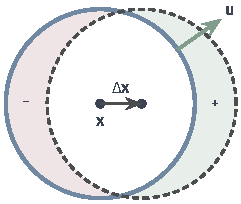
\includegraphics[width=41mm]{figures/05-optimization/05-stochastic-optimization/tikz/zo-disc-shift/figure.pdf}
  \caption{球平滑梯度的来历。蓝色实线是以$\bm{x}$为心的圆，虚线是平移$\Delta\bm{x}$后的圆。绿色月牙是新进入的区域，红色月牙是离开的区域，公共部分对积分的变化没有贡献。月牙在外法向$\bm{u}$处的厚度约为$\langle\Delta\bm{x},\bm{u}\rangle$。}
  \label{fig:zo-disc-shift}
\end{BookInlineFigure}

\begin{theorem}[球平滑的梯度恒等式]
\label{thm:zo-ball-identity}
设$f$在开集$\bm{U}$上连续，闭球$\bm{x}+\delta\bm{B}\subset\bm{U}$，$\bm{u}$在单位球面$\bm{S}$上均匀分布。则$f^{\mathrm{B}}_{\delta}$在$\bm{x}$处可微，且
\begin{equation}
 \nabla f^{\mathrm{B}}_{\delta}(\bm{x})=\frac{n}{\delta}\,\mathbb{E}_{\bm{u}}\bigl[f(\bm{x}+\delta\bm{u})\,\bm{u}\bigr].
 \label{eq:zo-ball-identity}
\end{equation}
\end{theorem}

\begin{proof}
先设$f$连续可微。可在积分号下求导，得
\[
 \partial_if^{\mathrm{B}}_{\delta}(\bm{x})=\frac{1}{\operatorname{vol}(\delta\bm{B})}\int_{\delta\bm{B}}\partial_if(\bm{x}+\bm{z})\,\mathrm{d}\bm{z}.
\]
对向量场$f(\bm{x}+\bm{z})\bm{e}_i$在球$\delta\bm{B}$上用散度定理，外法向是$\bm{z}/\delta$，于是
\[
 \partial_if^{\mathrm{B}}_{\delta}(\bm{x})=\frac{1}{\operatorname{vol}(\delta\bm{B})}\int_{\delta\bm{S}}f(\bm{x}+\bm{z})\frac{z_i}{\delta}\,\mathrm{d}S(\bm{z}).
\]

半径$\delta$的球体积是$c\,\delta^n$，对半径求导得球面积$nc\,\delta^{n-1}$，两者之比为$n/\delta$。把球面积分写成均匀分布下的期望，$\bm{z}=\delta\bm{u}$，就得到式~\eqref{eq:zo-ball-identity}。

再设$f$只连续。取$\bm{x}$的一个小邻域，使它的$\delta$膨胀的闭包是$\bm{U}$内的紧集，用光滑函数$f_k$在这个紧集上一致逼近$f$。$f_k$的平滑函数一致收敛到$f^{\mathrm{B}}_{\delta}$，它们的梯度由恒等式给出，一致收敛到式~\eqref{eq:zo-ball-identity}右端，右端关于位置连续。函数列一致收敛且导数列一致收敛时，极限函数可微且导数等于导数的极限。
\end{proof}

定理要求$f$连续，这个条件不能省。球面在球内的体积为零，把$f$在球面上的值任意修改，$f^{\mathrm{B}}_{\delta}$不变，式~\eqref{eq:zo-ball-identity}的右端却变了。恒等式右端要读取球面上的值，这些值必须与球内的值相联系，连续性保证了这一点。

\paragraph{估计器}
恒等式的右端是期望，抽一个方向就得到它的无偏样本。这称为\term{单点估计}（one-point estimator）：
\begin{equation}
 \hat{\bm{g}}^{(1)}=\frac{n}{\delta}\,y\,\bm{u},\qquad y=f(\bm{x}+\delta\bm{u}).
 \label{eq:zo-one-point}
\end{equation}
它每轮只需一次读数，单点接口也能用。读数含噪声时，只要给定历史、位置和方向时$\zeta$的条件均值为零，噪声项$\zeta\bm{u}$的均值就是零，估计的均值不变，仍是$\nabla f^{\mathrm{B}}_{\delta}(\bm{x})$。注意查询点在球面上，但被估计的是球内平均的梯度，两个集合不要混淆。

\paragraph{常数偏移改变二阶矩}
目标加一个常数$c$，梯度不变，估计的均值也不变，因为$\mathbb{E}[c\bm{u}]=\bm{0}$。可是估计本身变了。由$\lVert\bm{u}\rVert_2=1$，
\begin{equation}
 \mathbb{E}\lVert\hat{\bm{g}}^{(1)}\rVert_2^2=\frac{n^2}{\delta^2}\,\mathbb{E}\bigl[y^2\bigr],
 \label{eq:zo-one-point-moment}
\end{equation}
读数绝对值越大，二阶矩越大，哪怕它的大小与优化毫无关系。

贯穿例起点$f=45$，取$\delta=0.1$，$n=2$，因子$n/\delta=20$。沿$\pm\bm{e}_1$方向的两个估计是
\[
 \bm{u}=\bm{e}_1:\ (918.1,\ 0),\qquad\bm{u}=-\bm{e}_1:\ (-882.1,\ 0).
\]
沿$\pm\bm{e}_2$方向是
\[
 \bm{u}=\bm{e}_2:\ (0,\ 918.9),\qquad\bm{u}=-\bm{e}_2:\ (0,\ -882.9).
\]
四个向量的平均是$(9,9)$，等于真实梯度，但每个向量的长度约为$900$，比梯度长度$12.7$大七十倍。巨大的数相互抵消后才剩下需要的信号，如图~\ref{fig:zo-single-cloud}(a)。

如果事先知道$f$大约在$45$附近，把估计中的$y$换成$y-45$，均值不变，散布却缩回$20$左右，如图~\ref{fig:zo-single-cloud}(b)。可是这个常数算法事先并不知道，这就引出了下一小节的成对读数。

\begin{BookInlineFigure}
  \centering
  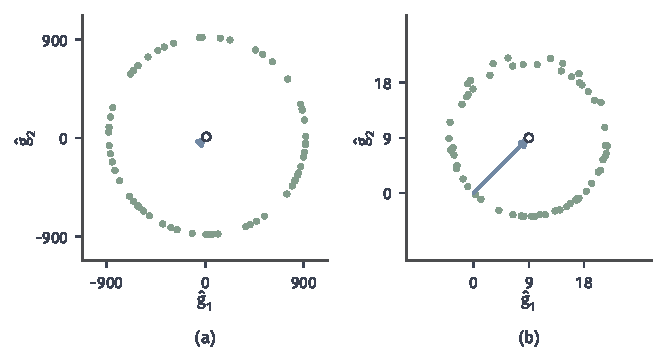
\includegraphics[width=112mm]{figures/05-optimization/05-stochastic-optimization/matplotlib/zo-single-cloud/figure.pdf}
  \caption{贯穿例起点的单点估计，$\delta=0.1$，$60$个随机方向。绿点是估计值，蓝色箭头是真实梯度$(9,9)$，空心圆是它的终点。(a)原读数的估计分布在半径约$900$的圆上，比梯度大两个量级。(b)读数减去常数$45$后，同样的$60$个方向给出的估计缩到半径约$13$的圆上。两张图的坐标范围不同。}
  \label{fig:zo-single-cloud}
\end{BookInlineFigure}

\paragraph{平滑目标的光滑常数}
单点估计常用于$f$只是$G$-Lipschitz的情形。这时$f^{\mathrm{B}}_{\delta}$是否光滑？由恒等式~\eqref{eq:zo-ball-identity}，对任意$\bm{x},\bm{z}$，
\[
 \lVert\nabla f^{\mathrm{B}}_{\delta}(\bm{x})-\nabla f^{\mathrm{B}}_{\delta}(\bm{z})\rVert_2
 \leq\frac{n}{\delta}\mathbb{E}\lvert f(\bm{x}+\delta\bm{u})-f(\bm{z}+\delta\bm{u})\rvert
 \leq\frac{nG}{\delta}\lVert\bm{x}-\bm{z}\rVert_2.
\]
所以$f^{\mathrm{B}}_{\delta}$的光滑常数不超过$nG/\delta$。$\delta$越小，平滑目标越接近原目标，但也越弯曲。这个上界不一定紧，它的作用是说明平滑后有光滑常数可用。

\subsection{双点估计}
\label{sec:zo-two-point}

成对查询允许把单点估计里的大数减掉。在相反方向各读一次，得到\term{双点估计}（two-point estimator）：
\begin{equation}
 \hat{\bm{g}}^{(2)}=\frac{n}{2\delta}\bigl(y_+-y_-\bigr)\bm{u},\qquad
 y_\pm=f(\bm{x}\pm\delta\bm{u}).
 \label{eq:zo-two-point}
\end{equation}
这正是第~\ref{sec:zo-random-direction}节的式~\eqref{eq:zo-random-direction}取$h=\delta$。公式相同，这里的解释却更精确。

\paragraph{为什么均值是平滑梯度}
$\bm{u}$和$-\bm{u}$同分布，所以单点估计用$-\bm{u}$代替$\bm{u}$，期望不变：
\[
 \frac{n}{\delta}\mathbb{E}\bigl[f(\bm{x}+\delta\bm{u})\bm{u}\bigr]
 =\frac{n}{\delta}\mathbb{E}\bigl[f(\bm{x}-\delta\bm{u})(-\bm{u})\bigr].
\]
两式相加除以$2$，右端正是$\mathbb{E}[\hat{\bm{g}}^{(2)}]$，左端由恒等式等于$\nabla f^{\mathrm{B}}_{\delta}(\bm{x})$。于是
\begin{equation}
 \mathbb{E}\bigl[\hat{\bm{g}}^{(2)}\bigr]=\nabla f^{\mathrm{B}}_{\delta}(\bm{x}).
 \label{eq:zo-two-point-mean}
\end{equation}

把两节的说法对照起来，同一个向量有两种读法。作为原梯度的近似，它有偏差，Hessian是Lipschitz时偏差是$O(\delta^2)$；作为平滑梯度的估计，它严格无偏。表~\ref{tab:zo-two-views}列出两种读法的差别。选哪种读法，取决于最终想回答关于哪个目标的问题。

\begin{BookInlineTable}
  \centering
  \begin{tabular}{@{}lll@{}}
    \toprule
    读法 & 估计对象 & 偏差\\
    \midrule
    有限差分 & $\nabla f(\bm{x})$ & 一般非零，随$\delta$缩小\\
    平滑估计 & $\nabla f^{\mathrm{B}}_{\delta}(\bm{x})$ & 严格为零\\
    \bottomrule
  \end{tabular}
  \caption{同一个双点向量的两种读法。原目标不可微时第一种读法没有对象，第二种仍然成立。}
  \label{tab:zo-two-views}
\end{BookInlineTable}

\paragraph{减去中心值的形式}
另一个双点形式把$y_-$换成中心读数：
\begin{equation}
 \hat{\bm{g}}^{(\mathrm{c})}=\frac{n}{\delta}\bigl(f(\bm{x}+\delta\bm{u})-f(\bm{x})\bigr)\bm{u}.
 \label{eq:zo-center-point}
\end{equation}
由$\mathbb{E}[f(\bm{x})\bm{u}]=\bm{0}$，它的均值也是$\nabla f^{\mathrm{B}}_{\delta}(\bm{x})$。两种形式都消除了常数偏移，贯穿例上把“很大的$45$”去掉了。

\paragraph{二阶矩的比较}
消去偏移后，估计的大小由差商决定。下面的引理针对光滑目标给出统一的界。

\begin{lemma}[双点估计的二阶矩]
\label{lem:zo-two-point-moment}
设$\nabla f$是$L$-Lipschitz的，读数精确。对估计~\eqref{eq:zo-two-point}和~\eqref{eq:zo-center-point}，都有
\begin{equation}
 \mathbb{E}\lVert\hat{\bm{g}}\rVert_2^2\leq 2n\lVert\nabla f(\bm{x})\rVert_2^2+\frac{n^2L^2\delta^2}{2}.
 \label{eq:zo-two-point-moment}
\end{equation}
\end{lemma}

\begin{proof}
记$\bm{g}=\nabla f(\bm{x})$，$\hat{\bm{g}}=nD\bm{u}$，其中$D$是对应的差商，写成$D=\langle\bm{g},\bm{u}\rangle+r$。由式~\eqref{eq:zo-central-L}或下降引理，两种形式都有$\lvert r\rvert\leq L\delta/2$。

用$(a+b)^2\leq2a^2+2b^2$和$\lVert\bm{u}\rVert_2=1$，
\[
 \lVert\hat{\bm{g}}\rVert_2^2=n^2D^2\leq 2n^2\langle\bm{g},\bm{u}\rangle^2+\frac{n^2L^2\delta^2}{2}.
\]
取期望，再用$\mathbb{E}[\bm{u}\bm{u}^\top]=\bm{I}/n$，得到结论。
\end{proof}

式~\eqref{eq:zo-two-point-moment}与单点的式~\eqref{eq:zo-one-point-moment}对比，分母里的$\delta^2$不见了，$\delta$可以取得很小而不使估计爆炸。这是精确读数下成对查询的实质收益。

两种双点形式的差别要看函数。贯穿例上，对称形式的差商精确等于方向导数，二阶矩是$n\lVert\bm{g}\rVert_2^2$；中心形式多出$\tfrac{\delta}{2}\bm{u}^\top\bm{H}\bm{u}$，二阶矩更大。在极小点$\bm{g}=\bm{0}$处，对称形式的估计恒为零，而中心形式不为零，这点上对称形式完全不抖动。$f=\lvert x\rvert$在$x=0$处，对称形式同样恒为零，中心形式的估计是$\pm1$。

但是“方差改善”不是无条件的结论。第一，改善来自消去$f$的大小，如果$f$本身在零附近，单点估计并没有这部分额外的方差。第二，带独立噪声时，两次单点估计取平均与一次双点估计噪声贡献相同，都是$n^2\sigma^2/(2\delta^2)$，第~\ref{sec:zo-pair-noise}节会算出来。所以成对读数消去的是函数值的公共部分，不是噪声。

\subsection{高斯方向估计}
\label{sec:zo-gaussian}

球面方向需要扰动恰好落在半径$\delta$的球面上。如果改用高斯扰动，查询点不再被限制在球面上，分析也更简单，因为高斯密度的导数有封闭形式。

\paragraph{主要思想}
作变量替换$\bm{z}=\bm{x}+\tau\bm{w}$，把高斯平滑写成
\[
 f^{\mathrm{G}}_{\tau}(\bm{x})=\frac{1}{(2\pi\tau^2)^{n/2}}\int f(\bm{z})\exp\Bigl(-\frac{\lVert\bm{z}-\bm{x}\rVert_2^2}{2\tau^2}\Bigr)\mathrm{d}\bm{z}.
\]
现在$\bm{x}$只出现在指数里，$f$不必可微，梯度全部落到光滑的高斯核上。这与球平滑的情况类似：导数从$f$转移到了平均方式上。

\begin{theorem}[高斯平滑的梯度恒等式]
\label{thm:zo-gauss-identity}
设$f$可测，存在$C,a\geq0$使$\lvert f(\bm{z})\rvert$处处不超过$Ce^{a\lVert\bm{z}\rVert_2}$，$\bm{w}\sim\mathcal{N}(\bm{0},\bm{I})$。则$f^{\mathrm{G}}_{\tau}$可微，且
\begin{equation}
 \nabla f^{\mathrm{G}}_{\tau}(\bm{x})=\frac{1}{\tau}\,\mathbb{E}_{\bm{w}}\bigl[f(\bm{x}+\tau\bm{w})\,\bm{w}\bigr].
 \label{eq:zo-gauss-identity}
\end{equation}
\end{theorem}

\begin{proof}
高斯核对$\bm{x}$的梯度等于核本身乘$(\bm{z}-\bm{x})/\tau^2$。当$\bm{x}$在一个有界邻域内时，被积函数对$\bm{x}$的梯度被一个不依赖$\bm{x}$的可积函数控制：指数增长被高斯衰减压住。由控制收敛定理，可在积分号下求导，得
\[
 \nabla f^{\mathrm{G}}_{\tau}(\bm{x})=\frac{1}{(2\pi\tau^2)^{n/2}}\int f(\bm{z})\frac{\bm{z}-\bm{x}}{\tau^2}\exp\Bigl(-\frac{\lVert\bm{z}-\bm{x}\rVert_2^2}{2\tau^2}\Bigr)\mathrm{d}\bm{z}.
\]
再换回$\bm{z}=\bm{x}+\tau\bm{w}$，$(\bm{z}-\bm{x})/\tau^2=\bm{w}/\tau$，即得结论。
\end{proof}

这个定理比球面的恒等式要求的局部性质弱：$f$可以不连续，因为积分覆盖整个空间，$f$在零测集上的值不起作用。要求转移到了全局的增长上，这正好是定义中高斯平滑存在所需要的。

\paragraph{三种形式}
抽一个$\bm{w}$，式~\eqref{eq:zo-gauss-identity}给出单点形式。与球面的情形一样，减去中心值或取对称差，均值不变：
\begin{equation}
 \hat{\bm{g}}^{\mathrm{G}}=\frac{y}{\tau}\bm{w},\qquad
 \hat{\bm{g}}^{\mathrm{Gc}}=\frac{y-f(\bm{x})}{\tau}\bm{w},\qquad
 \hat{\bm{g}}^{\mathrm{Gs}}=\frac{y-y'}{2\tau}\bm{w},
 \label{eq:zo-gauss-estimators}
\end{equation}
其中$y=f(\bm{x}+\tau\bm{w})$，$y'=f(\bm{x}-\tau\bm{w})$。第二种利用了$\mathbb{E}[\bm{w}]=\bm{0}$，第三种利用了$\bm{w}$与$-\bm{w}$同分布。

贯穿例起点，取$\tau=0.1$，抽到$\bm{w}=(1,-0.5)$。对称形式的读数和差商是
\[
 f(9.1,0.95)=45.46625,\qquad f(8.9,1.05)=44.56625,\qquad\frac{y-y'}{2\tau}=4.5.
\]
这里$\langle\nabla f,\bm{w}\rangle=9-4.5=4.5$，吻合。估计是$4.5\,\bm{w}=(4.5,-2.25)$。

\paragraph{与球面方向的区别}
公式里没有因子$n$，这是因为$\mathbb{E}[\bm{w}\bm{w}^\top]=\bm{I}$，球面方向则是$\bm{I}/n$。如果把球面的归一化照搬过来写成$(n/\tau)y\bm{w}$，二次函数上的均值就变成$n\nabla f$，整整放大$n$倍。

另一个区别是扰动的长度。$\lVert\bm{w}\rVert_2$是随机的，大约是$\sqrt{n}$，如图~\ref{fig:zo-sphere-gauss}(b)。$\tau$只是尺度，不是查询半径。$n=2$时
\[
 \mathbb{P}\bigl(\lVert\bm{w}\rVert_2>3\bigr)=e^{-4.5}\approx0.011,
\]
一百次里约有一次偏离三个尺度。要与球面半径$\delta$对应，应取$\tau=\delta/\sqrt{n}$，这时$\tau\bm{w}$的均方长度等于$\delta^2$。

\begin{BookInlineFigure}
  \centering
  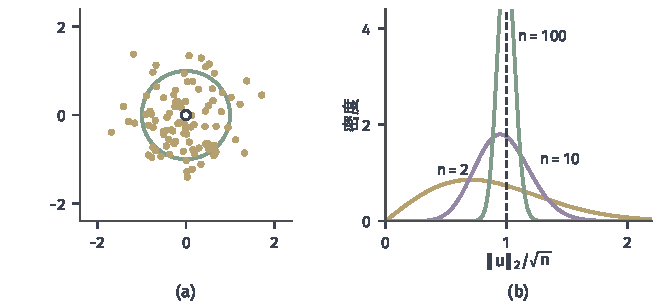
\includegraphics[width=112mm]{figures/05-optimization/05-stochastic-optimization/matplotlib/zo-sphere-gauss/figure.pdf}
  \caption{球面方向与高斯方向。(a)$n=2$，绿圆是半径$\delta=1$的球面查询位置，黄点是尺度$\tau=1/\sqrt{2}$的高斯查询点，二者均方长度相同，高斯点散布在圆内外。(b)$\lVert\bm{w}\rVert_2/\sqrt{n}$的密度。维数增大时高斯方向的长度集中到$\sqrt{n}$附近，$n=2$时差异很大。}
  \label{fig:zo-sphere-gauss}
\end{BookInlineFigure}

二次函数上，对称形式的二阶矩可以直接算：
\[
 \mathbb{E}\bigl[\langle\bm{g},\bm{w}\rangle^2\lVert\bm{w}\rVert_2^2\bigr]=(n+2)\lVert\bm{g}\rVert_2^2.
\]
所以方差是$(n+1)\lVert\bm{g}\rVert_2^2$，比球面方向的$(n-1)\lVert\bm{g}\rVert_2^2$略大，多出来的部分来自长度的波动。一般光滑函数上有类似的上界：
\begin{equation}
 \mathbb{E}\lVert\hat{\bm{g}}^{\mathrm{Gs}}\rVert_2^2\leq2(n+2)\lVert\nabla f(\bm{x})\rVert_2^2+\frac{L^2\tau^2}{2}n(n+2)(n+4).
 \label{eq:zo-gauss-moment}
\end{equation}
推导与引理~\ref{lem:zo-two-point-moment}相同，只是余项是$\lvert r\rvert\leq L\tau\lVert\bm{w}\rVert_2^2/2$，再用高斯矩$\mathbb{E}\lVert\bm{w}\rVert_2^6=n(n+2)(n+4)$。

\subsection{成对读数的噪声}
\label{sec:zo-pair-noise}

到此为止的二阶矩都假设读数精确。本小节回到第~\ref{sec:zo-pair-interface}节的接口问题：读数含噪声时，成对差分的波动是多少？

\paragraph{独立噪声}
采用式~\eqref{eq:zo-independent-pair}，$\zeta_+,\zeta_-$条件独立，均值零，方差不超过$\sigma^2$。差商的噪声部分是$(\zeta_+-\zeta_-)/(2\delta)$，于是
\begin{equation}
 \operatorname{Var}\Bigl(\frac{\zeta_+-\zeta_-}{2\delta}\Bigr)\leq\frac{\sigma^2}{2\delta^2}.
 \label{eq:zo-independent-variance}
\end{equation}
半径减半，方差变成四倍。噪声大小不随距离变小，分母却在变小。图~\ref{fig:zo-pair-noise}中黄线的斜率是$-2$。

噪声与差商主项的交叉项为零，因为噪声的条件均值是零。代入估计，$\lVert\hat{\bm{g}}^{(2)}\rVert_2^2$的期望增加$n^2\sigma^2/(2\delta^2)$。结合引理~\ref{lem:zo-two-point-moment}，得到后面反复使用的二阶矩界：
\begin{equation}
 \mathbb{E}\lVert\hat{\bm{g}}^{(2)}\rVert_2^2\leq2n\lVert\nabla f(\bm{x})\rVert_2^2+V,\qquad
 V=\frac{n^2L^2\delta^2}{2}+\frac{n^2\sigma^2}{2\delta^2}.
 \label{eq:zo-noisy-moment}
\end{equation}

\paragraph{单点平均与成对差分}
单点估计用两次独立读数和两个独立方向取平均时，噪声贡献是
\[
 \frac14\Bigl(\frac{n^2\sigma^2}{\delta^2}+\frac{n^2\sigma^2}{\delta^2}\Bigr)=\frac{n^2\sigma^2}{2\delta^2},
\]
与双点估计完全相同。这验证了前面的说法：独立噪声下，配对不减少噪声，只消去函数值的公共部分。

\paragraph{共享样本}
采用式~\eqref{eq:zo-shared-pair}，差分的方差包含协方差：
\begin{equation}
 \operatorname{Var}\bigl[F(\bm{q}_+;\bm{\xi})-F(\bm{q}_-;\bm{\xi})\bigr]
 =\operatorname{Var}F_++\operatorname{Var}F_--2\operatorname{Cov}(F_+,F_-).
 \label{eq:zo-shared-variance}
\end{equation}
共享样本带来的是正的协方差，协方差越大，抵消越多。若两个噪声的相关系数是$\rho$且方差都是$\sigma^2$，差的方差是$2\sigma^2(1-\rho)$，从$\rho=0$的独立到$\rho=1$的完全抵消，中间是连续变化的。

\paragraph{三个例子}
共享样本的效果取决于样本函数本身的波动。

第一个例子是两点共享同一个加性噪声，$F(\bm{x};\xi)=f(\bm{x})+\xi$。差分时$\xi$完全消失，噪声方差为零，无论半径多小，差商都是精确的。

第二个例子是样本函数关于$\bm{x}$Lipschitz，比如$F(\bm{x};\bm{\xi})=f(\bm{x})+\bm{\xi}^\top\bm{x}$。差分的随机部分是
\[
 \frac{\bm{\xi}^\top(\bm{q}_+-\bm{q}_-)}{2\delta}=\bm{\xi}^\top\bm{u},
\]
它不依赖$\delta$。一般地，若$F(\cdot;\bm{\xi})$是Lipschitz的，常数为$G(\bm{\xi})$，差商的二阶矩不超过$\mathbb{E}[G(\bm{\xi})^2]$，$\delta$可以取得很小。图~\ref{fig:zo-pair-noise}中绿线是水平的。

第三个例子是样本函数不连续。$F(x;\xi)=\mathbb{1}\{x>\xi\}$，$\xi$的密度为$p$。共享$\xi$时差分只在$\xi\in[x-h,x+h)$时非零，概率约$2hp(x)$，于是差商方差约为
\[
 \frac{2hp(x)}{4h^2}=\frac{p(x)}{2h}.
\]
它比独立噪声的$1/h^2$好，但仍随$h$缩小而增大，图~\ref{fig:zo-pair-noise}中紫线的斜率是$-1$。所以共享样本带来改善的前提是差值的波动受控，只说“用了同一个种子”并不够。

\begin{BookInlineFigure}
  \centering
  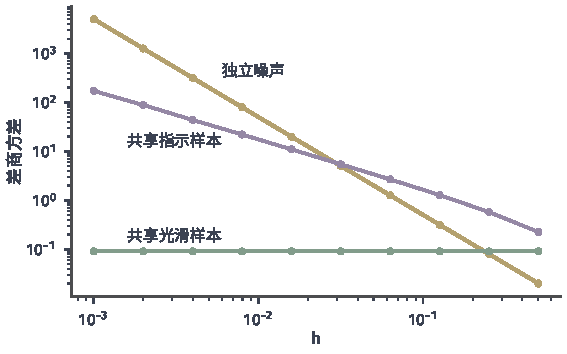
\includegraphics[width=96mm]{figures/05-optimization/05-stochastic-optimization/matplotlib/zo-pair-noise/figure.pdf}
  \caption{中心差商的方差随$h$的变化，$x=0.5$。黄线：独立加性噪声，标准差$0.1$，斜率$-2$。紫线：共享指示样本$F=\mathbb{1}\{x>\xi\}$，$\xi\sim\mathcal{N}(0,1)$，斜率$-1$。绿线：共享光滑样本$F=x^2/2+\xi x$，$\xi$标准差$0.3$，方差不随$h$变化。共享同一加性噪声时方差为零，未画出。每点来自$4\times10^6$次模拟。}
  \label{fig:zo-pair-noise}
\end{BookInlineFigure}

\section{零阶随机梯度方法}
\label{sec:zo-method}

前两节构造了各种方向估计。接下来要弄清：把它们放进迭代后，算法实际在优化什么，步长和扰动尺度怎样定，遇到约束怎么办，最后交出什么结果？

\subsection{基本迭代}
\label{sec:zo-basic}

\paragraph{主要思想}
第~\ref{chap:stochastic-gradient-methods}章的随机更新沿随机方向$\hat{\bm{g}}^{(t)}$的负向走一步。它能用的原因是，这个方向平均起来指向某个函数的梯度。零阶方法沿用这个更新，只是$\hat{\bm{g}}^{(t)}$由函数值算出：
\begin{equation}
 \bm{x}^{(t+1)}=\bm{x}^{(t)}-\alpha^{(t)}\hat{\bm{g}}^{(t)},\qquad
 \hat{\bm{g}}^{(t)}=\frac{n}{2\delta}\bigl(y_+^{(t)}-y_-^{(t)}\bigr)\bm{u}^{(t)}.
 \label{eq:zo-update}
\end{equation}
这是\term{零阶随机梯度方法}（zeroth-order stochastic gradient method）的双点形式，其他估计器可以替换第二式。一轮的流程如图~\ref{fig:zo-flow}所示。

\begin{BookInlineFigure}
  \centering
  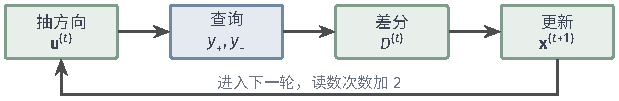
\includegraphics[width=105mm]{figures/05-optimization/05-stochastic-optimization/tikz/zo-flow/figure.pdf}
  \caption{双点零阶方法的一轮。绿框是算法内部的计算，蓝框是向黑箱提交的查询。每轮两次函数读数，查询预算按读数次数累计。}
  \label{fig:zo-flow}
\end{BookInlineFigure}

更新形式都一样，算法朝哪里走却由估计器的条件均值决定，不能只看形式。式~\eqref{eq:zo-update}的条件均值是$\nabla f^{\mathrm{B}}_{\delta}(\bm{x}^{(t)})$，所以它是平滑目标上的随机梯度方法，不是原目标上的。

\needspace{6\baselineskip}
\paragraph{变量}
\begin{itemize}
 \item $\bm{x}^{(t)}\in\mathbb{R}^n$：当前迭代点。
 \item $\bm{u}^{(t)}\in\bm{S}$：本轮的单位方向，$n$维。
 \item $y_\pm^{(t)}$：两次读数，标量。
 \item $D^{(t)}=(y_+^{(t)}-y_-^{(t)})/(2\delta)$：差商，标量。
 \item $\hat{\bm{g}}^{(t)}\in\mathbb{R}^n$：方向估计。
 \item $\alpha$、$\delta$：步长与扰动半径，取常数。
 \item $Q$：已用读数次数。
\end{itemize}

\paragraph{初始化}
取起点$\bm{x}^{(0)}$，选定$\alpha$、$\delta$和读数预算$Q_{\max}$，令$Q=0$。例中目标是贯穿例~\eqref{eq:zo-example}，读数带独立噪声，并取
\[
 \bm{x}^{(0)}=(9,1),\quad\alpha=0.05,\quad\delta=0.5,\quad Q_{\max}=6.
\]

\needspace{6\baselineskip}
\paragraph{每轮更新}
下面的数值用事先给定的方向和噪声，便于逐项核对。
\begin{enumerate}
 \item 抽取方向$\bm{u}^{(t)}$。例中第一轮$\bm{u}^{(0)}=(0.6,0.8)$，第二轮$\bm{u}^{(1)}=(0.8,-0.6)$，第三轮$\bm{u}^{(2)}=(0.28,0.96)$。
 \item 查询$\bm{x}^{(t)}\pm\delta\bm{u}^{(t)}$，$Q$增加$2$。例中第一轮两个查询点是$(9.3,1.4)$和$(8.7,0.6)$，真实函数值为$52.065$和$39.465$，噪声分别为$+0.1$和$-0.1$，读数是
 \[
  y_+^{(0)}=52.165,\qquad y_-^{(0)}=39.365.
 \]
 \item 由式~\eqref{eq:zo-update}算差商和方向估计。例中$2\delta=1$，$n=2$，第一轮结果是
 \[
  D^{(0)}=12.8,\qquad\hat{\bm{g}}^{(0)}=2\cdot12.8\cdot(0.6,0.8)=(15.36,\ 20.48).
 \]
 \item 由式~\eqref{eq:zo-update}沿$-\hat{\bm{g}}^{(t)}$走步长$\alpha$。例中第一轮得到
 \[
  \bm{x}^{(1)}=(9,1)-0.05\,(15.36,20.48)=(8.232,\ -0.024).
 \]
\end{enumerate}

第二轮从$\bm{x}^{(1)}$出发，查询点是$(8.632,-0.324)$和$(7.832,0.276)$，噪声是$-0.1$和$+0.1$，读数和结果为
\[
 y_+^{(1)}\approx37.628,\quad y_-^{(1)}\approx31.113,\quad D^{(1)}\approx6.515,
\]
\[
 \hat{\bm{g}}^{(1)}\approx(10.424,\ -7.818),\qquad\bm{x}^{(2)}\approx(7.711,\ 0.367).
\]

第三轮查询点是$(7.851,0.847)$和$(7.571,-0.113)$，噪声是$+0.05$和$+0.15$，读数和结果为
\[
 y_+^{(2)}\approx34.095,\quad y_-^{(2)}\approx28.866,\quad D^{(2)}\approx5.229,
\]
\[
 \hat{\bm{g}}^{(2)}\approx(2.928,\ 10.040),\qquad\bm{x}^{(3)}\approx(7.564,\ -0.135).
\]

迭代在$Q$达到$Q_{\max}$时结束。例中三轮用完$6$次读数，最终得到$\bm{x}^{(3)}\approx(7.564,-0.135)$，真实目标值约$28.69$，从$45$下降了三分之一多。第二轮的梯度第二分量只有$-0.216$，估计的第二分量却是$-7.818$，$x_2$从$-0.024$跳到$0.367$，这种摆动是单方向估计的常态。继续运行的结果见图~\ref{fig:zo-paths}。

\begin{BookInlineFigure}
  \centering
  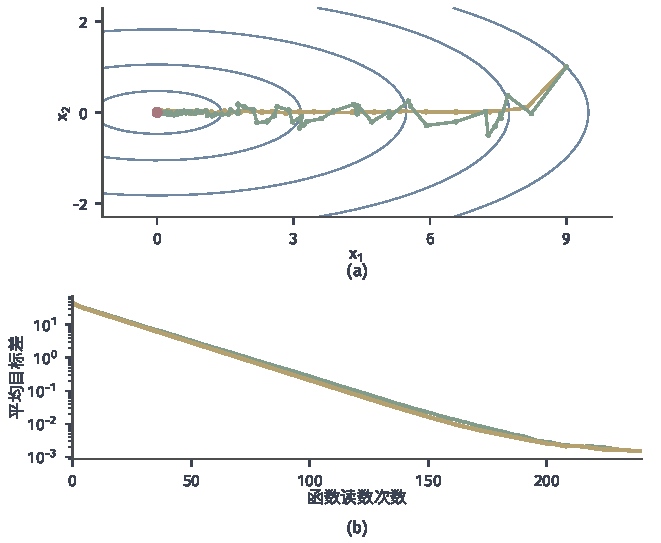
\includegraphics[width=112mm]{figures/05-optimization/05-stochastic-optimization/matplotlib/zo-paths/figure.pdf}
  \caption{贯穿例上的零阶迭代，读数噪声标准差$0.1$。(a)绿线是双点球面方法的一次运行，$\alpha=0.05$，$\delta=0.5$，前三轮即正文手算的数据，共$120$轮；黄线是中心坐标差分的梯度下降，$\alpha=0.1$，$h=0.5$，共$60$轮；蓝线是等高线，红点是解。(b)$200$次运行的平均目标差，横轴是函数读数次数。}
  \label{fig:zo-paths}
\end{BookInlineFigure}

图~\ref{fig:zo-paths}(a)中绿线抖动，黄线平稳，但按读数次数算两者几乎重合，如图~\ref{fig:zo-paths}(b)。这里两者的步长不同：单方向估计的步长要比完整梯度小一个与$n$相关的倍数，原因在第~\ref{sec:zo-step-scale}节说明。

\paragraph{多方向平均}
每轮抽$m$个独立方向，分别计算估计后取平均，是最常见的变体，一轮用$2m$次读数：
\begin{equation}
 \hat{\bm{g}}^{(t)}=\frac{1}{m}\sum_{j=1}^{m}\frac{n}{2\delta}\bigl(y_{j,+}^{(t)}-y_{j,-}^{(t)}\bigr)\bm{u}_j^{(t)}.
 \label{eq:zo-multi-direction}
\end{equation}
条件均值不变，方差变成$1/m$。例中第一轮若用$\bm{u}_1=(0.6,0.8)$和$\bm{u}_2=(0.8,-0.6)$两个方向，不计噪声时，两个估计是
\[
 (15.12,\ 20.16),\qquad(2.88,\ -2.16).
\]
它们的平均恰为$(9,9)$，这时$\bm{x}^{(1)}=(8.55,0.55)$。两个方向正交且数量等于维数，对二次函数恰好拼出了完整梯度。

\paragraph{一步分析：有偏与无偏两条路}
把估计器代入迭代，有两种分析方式，对应前面的两种读法。先假设$\nabla f$是$L$-Lipschitz的，第一种直接看原目标。

\begin{lemma}[单步下降]
\label{lem:zo-one-step}
设$\bm{x}^+=\bm{x}-\alpha\hat{\bm{g}}$，$\nabla f$是$L$-Lipschitz的。若$\hat{\bm{g}}$的条件均值是$\nabla f(\bm{x})+\bm{b}$，且$\lVert\bm{b}\rVert_2\leq\beta$，则
\begin{equation}
 \mathbb{E}[f(\bm{x}^+)\mid\bm{x}]\leq f(\bm{x})-\frac{\alpha}{2}\lVert\nabla f(\bm{x})\rVert_2^2+\frac{\alpha}{2}\beta^2+\frac{L\alpha^2}{2}\mathbb{E}\bigl[\lVert\hat{\bm{g}}\rVert_2^2\mid\bm{x}\bigr].
 \label{eq:zo-biased-step}
\end{equation}
若$\hat{\bm{g}}$的条件均值是$\nabla f^{\mathrm{B}}_{\delta}(\bm{x})$，则
\begin{equation}
 \mathbb{E}[f^{\mathrm{B}}_{\delta}(\bm{x}^+)\mid\bm{x}]\leq f^{\mathrm{B}}_{\delta}(\bm{x})-\alpha\lVert\nabla f^{\mathrm{B}}_{\delta}(\bm{x})\rVert_2^2+\frac{L\alpha^2}{2}\mathbb{E}\bigl[\lVert\hat{\bm{g}}\rVert_2^2\mid\bm{x}\bigr].
 \label{eq:zo-unbiased-step}
\end{equation}
\end{lemma}

\begin{proof}
由下降引理，对$L$-光滑函数$\psi$，
\[
 \psi(\bm{x}^+)\leq\psi(\bm{x})-\alpha\langle\nabla\psi(\bm{x}),\hat{\bm{g}}\rangle+\frac{L\alpha^2}{2}\lVert\hat{\bm{g}}\rVert_2^2.
\]
取$\psi=f$并取条件期望，内积项变为$-\alpha\lVert\nabla f\rVert_2^2-\alpha\langle\nabla f,\bm{b}\rangle$。再用
\[
 -\langle\nabla f,\bm{b}\rangle\leq\frac12\lVert\nabla f\rVert_2^2+\frac12\beta^2,
\]
得式~\eqref{eq:zo-biased-step}。

取$\psi=f^{\mathrm{B}}_{\delta}$，由引理~\ref{lem:zo-smoothing-properties}，它也是$L$-光滑的，内积项的条件期望是$-\alpha\lVert\nabla f^{\mathrm{B}}_{\delta}\rVert_2^2$，得式~\eqref{eq:zo-unbiased-step}。
\end{proof}

两式对比可以看出两种分析的差别。式~\eqref{eq:zo-biased-step}留下了偏差项$\tfrac{\alpha}{2}\beta^2$，它每步都存在，累加后构成不会随步数消失的误差。式~\eqref{eq:zo-unbiased-step}没有偏差项，账记在平滑目标上，代价是结论说的是$f^{\mathrm{B}}_{\delta}$，要回到$f$还须另算，这留给第~\ref{sec:zo-original-error}节。

\subsection{步长与扰动尺度}
\label{sec:zo-step-scale}

这里有两个旋钮。步长$\alpha$决定参数实际走多远，扰动尺度$\delta$决定在多大的邻域里比较函数值。两者的量纲都不同：改变$\delta$不移动$\bm{x}$，只改变估计的性质。

\paragraph{步长的上限}
由式~\eqref{eq:zo-noisy-moment}，二阶矩中有$2n\lVert\nabla f\rVert_2^2$，比完整梯度的$\lVert\nabla f\rVert_2^2$大$2n$倍。代入式~\eqref{eq:zo-unbiased-step}，要让下降项压住二阶矩项，需要$\alpha\lesssim1/(nL)$。直观地说，估计的长度波动约为梯度的$\sqrt{n}$倍，步长必须相应地收小。

这个步长要与每轮的读数次数放在一起看。完整坐标差分的步长是$1/L$，但每轮要$2n$次读数；单方向的步长是$1/(nL)$，每轮$2$次读数。按读数次数算，两者每次读数的“进展”同阶，这就是图~\ref{fig:zo-paths}(b)中两条曲线重合的原因。

贯穿例的手算用了$\alpha=0.05<1/(nL)=1/18$。下一小节定理要求的$\alpha\leq1/(4nL)=1/72$更保守，这是为了在任意光滑函数上保证下降，实际使用时常可放宽。

\paragraph{固定尺度对应固定的平滑目标}
$\delta$固定时，迭代是同一个$f^{\mathrm{B}}_{\delta}$上的随机梯度方法，所以固定步长最终会停在一个噪声水平上。图~\ref{fig:zo-delta-floor}(a)在贯穿例上取$\alpha=0.02$，噪声$\sigma=1$，分别用$\delta=0.1,0.5,2$。

三条曲线下降段相同，稳定后的水平差别很大，$\delta$从$0.1$增大到$0.5$，水平约下降$25$倍。这正是式~\eqref{eq:zo-noisy-moment}中$V$的噪声项$n^2\sigma^2/(2\delta^2)$的$1/\delta^2$规律。这个例子是二次函数，平滑没有引入任何偏差，所以$\delta$越大越好；一般函数上$\delta$还有偏差的代价，第~\ref{sec:zo-tradeoff}节讨论。

\begin{BookInlineFigure}
  \centering
  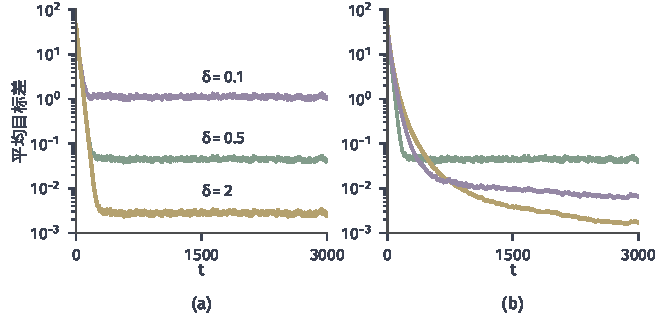
\includegraphics[width=112mm]{figures/05-optimization/05-stochastic-optimization/matplotlib/zo-delta-floor/figure.pdf}
  \caption{贯穿例上双点方法的平均目标差，读数噪声$\sigma=1$，$300$次运行。(a)固定$\alpha=0.02$，紫、绿、黄三线分别为$\delta=0.1,0.5,2$，稳定水平按$1/\delta^2$变化。(b)$\delta=0.5$时固定$\alpha=0.02$（绿）；步长递减$\alpha^{(t)}=0.02/(1+t/100)$（黄）；步长递减较慢、尺度也递减，$\alpha^{(t)}=0.02/(1+t/100)^{0.75}$，$\delta^{(t)}=0.5/(1+t/100)^{0.1}$（紫）。}
  \label{fig:zo-delta-floor}
\end{BookInlineFigure}

\paragraph{递减步长}
要越过这个水平，步长必须递减，这与第~\ref{chap:stochastic-gradient-methods}章的情形相同。图~\ref{fig:zo-delta-floor}(b)的黄线就是在$\delta$固定时让步长递减，曲线继续下降。

\paragraph{逐步缩小尺度要多记两笔}
既然小的$\delta$偏差小，能否让$\delta^{(t)}$随迭代缩小？可以，但目标函数本身在变，分析要多记两笔。

第一笔是目标的变化。第$t$步看的是$f^{\mathrm{B}}_{\delta^{(t)}}$，下一步换成$f^{\mathrm{B}}_{\delta^{(t+1)}}$，累加时不再是同一个函数相减，多出差值$f^{\mathrm{B}}_{\delta^{(t+1)}}-f^{\mathrm{B}}_{\delta^{(t)}}$。若$\delta^{(t+1)}\leq\delta^{(t)}$，由式~\eqref{eq:zo-ball-error}，这个差值的绝对值不超过$L(\delta^{(t)})^2$，一般情形要把它们加起来，$\sum_t(\delta^{(t)})^2$必须受控。

凸函数的情形方便一些。设$\delta_1\leq\delta_2$，$\lambda=\delta_1/\delta_2$。由凸性，
\[
 f(\bm{x}+\delta_1\bm{v})\leq\lambda f(\bm{x}+\delta_2\bm{v})+(1-\lambda)f(\bm{x}).
\]
取期望并用$f\leq f^{\mathrm{B}}_{\delta_2}$，得
\[
 f^{\mathrm{B}}_{\delta_1}\leq f^{\mathrm{B}}_{\delta_2}.
\]
所以缩小半径时平滑目标只降不升，这一笔差值对凸函数不造成损失。

第二笔是方差的变化。$V$里的噪声项是$n^2\sigma^2/(2(\delta^{(t)})^2)$，缩小$\delta$会放大方差，步长必须缩得更快，抵消这部分增长。累加式~\eqref{eq:zo-unbiased-step}可见需要控制的是$\sum_t(\alpha^{(t)})^2V^{(t)}$，因此独立噪声下的标准要求是
\begin{equation}
 \sum_t\alpha^{(t)}=\infty,\qquad
 \sum_t\Bigl(\frac{\alpha^{(t)}}{\delta^{(t)}}\Bigr)^2<\infty,\qquad
 \delta^{(t)}\to0.
 \label{eq:zo-schedule}
\end{equation}
前一个条件保证能走得足够远，后一个条件是随机逼近步长条件的变形\scite{math-robbins1951stochastic}，分母上多了$\delta^{(t)}$，反映差商的噪声放大。图~\ref{fig:zo-delta-floor}(b)的紫线步长递减更慢，尺度也在缩小，两者都使噪声项更大，所以高于黄线。这个二次函数上$\delta$没有偏差可减，缩小尺度没有收益，这也说明$\delta$是否该缩小要看偏差。

\subsection{约束下的查询}
\label{sec:zo-constrained-query}

约束问题要多考虑一件事：不光更新点要可行，查询点也可能需要可行。仿真器在非法参数下可能崩溃，物理实验在限制之外可能损坏设备。

\paragraph{更新可行不等于查询可行}
投影更新
\[
 \bm{x}^{(t+1)}=\Pi_{\bm{C}}\bigl(\bm{x}^{(t)}-\alpha\hat{\bm{g}}^{(t)}\bigr)
\]
保证了迭代点在$\bm{C}$内，但没有限制查询点。以$\bm{C}=[1,9]\times[-1,1]$为例，$\bm{x}=(1,0.4)$在边界上，取$\delta=0.2$，$\bm{u}=(0.6,0.8)$，两个查询点是
\[
 \bm{x}+\delta\bm{u}=(1.12,\ 0.56),\qquad\bm{x}-\delta\bm{u}=(0.88,\ 0.24).
\]
第二个点的$x_1<1$，越出了可行域，如图~\ref{fig:zo-constrained}(a)。投影把迭代点拉回来，却管不到这一步。

\begin{BookInlineFigure}
  \centering
  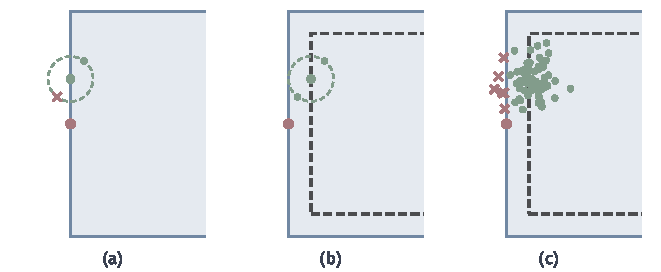
\includegraphics[width=112mm]{figures/05-optimization/05-stochastic-optimization/matplotlib/zo-constrained/figure.pdf}
  \caption{可行域$\bm{C}=[1,9]\times[-1,1]$的左端（浅蓝），红点是贯穿例在$\bm{C}$上的解$(1,0)$，绿点是迭代点和可行的查询点，红叉是越界查询。(a)迭代点在边界上，半径$0.2$的查询圆（绿色虚线）越界，$(0.88,0.24)$不可行。(b)把迭代点限制在内缩域（灰色虚线），查询圆完全在$\bm{C}$内。(c)同样的内缩域，尺度$\tau=\delta/\sqrt{2}$的高斯扰动仍有查询点越界。}
  \label{fig:zo-constrained}
\end{BookInlineFigure}

\paragraph{收缩查询区域}
解决办法是把迭代点限制在一个内缩的区域里，让半径$\delta$的球放得下。设凸集$\bm{C}$含有以原点为心、半径$r$的球，即$r\bm{B}\subseteq\bm{C}$。令$\theta=\delta/r\in(0,1)$，取收缩集合
\begin{equation}
 \bm{C}_\theta=(1-\theta)\bm{C}.
 \label{eq:zo-shrink}
\end{equation}

\begin{theorem}[收缩集合的查询可行性与边界误差]
\label{thm:zo-shrink}
设$\bm{C}$是凸集，$r\bm{B}\subseteq\bm{C}$，$\theta=\delta/r<1$。则对$\bm{x}\in\bm{C}_\theta$和$\bm{v}\in\bm{B}$，有$\bm{x}+\delta\bm{v}\in\bm{C}$。若$f$在$\bm{C}$上是凸函数，$\bm{x}^\star\in\bm{C}$是解，则
\begin{equation}
 \min_{\bm{x}\in\bm{C}_\theta}f(\bm{x})-f^\star\leq\theta\bigl(f(\bm{0})-f^\star\bigr).
 \label{eq:zo-shrink-error}
\end{equation}
\end{theorem}

\begin{proof}
设$\bm{x}=(1-\theta)\bm{c}$，$\bm{c}\in\bm{C}$。则
\[
 \bm{x}+\delta\bm{v}=(1-\theta)\bm{c}+\theta\,(r\bm{v}),
\]
这里用了$\delta=\theta r$。右端是$\bm{C}$中两点$\bm{c}$和$r\bm{v}$的凸组合，所以在$\bm{C}$中。

误差界：$(1-\theta)\bm{x}^\star\in\bm{C}_\theta$，由凸性，
\[
 f\bigl((1-\theta)\bm{x}^\star+\theta\bm{0}\bigr)\leq(1-\theta)f^\star+\theta f(\bm{0}).
\]
移项即得。
\end{proof}

定理的条件中，内部球不可少：$r$越小，同样的$\delta$需要收缩得越多，$\bm{C}$没有内点时完全无法在$\bm{C}$内做全维扰动。凸性用在了两处，凸组合的可行性和最后的误差界。

继续上面的例子，以$(5,0)$为中心平移，$\bm{C}$含半径$r=1$的球。$\delta=0.2$时$\theta=0.2$，$\bm{C}_\theta=[1.8,8.2]\times[-0.8,0.8]$。解$(1,0)$被挡在外面，$\bm{C}_\theta$上最好的点是$(1.8,0)$，代价是$f(1.8,0)-f(1,0)=1.12$，定理的上界是$0.2\cdot(12.5-0.5)=2.4$。按比例收缩对长边很不划算。

如果知道$\bm{C}$的形状，直接用内缩集$\{\bm{x}:\bm{x}+\delta\bm{B}\subseteq\bm{C}\}$更好。这里它是$[1.2,8.8]\times[-0.8,0.8]$，如图~\ref{fig:zo-constrained}(b)，代价只有$f(1.2,0)-f(1,0)=0.22$。

收缩产生的误差要计入最终结果：算法解的是$\bm{C}_\theta$上的问题，$\delta$越大这笔误差越大，同时噪声方差越小，这是约束情形下多出来的一层取舍。

\paragraph{高斯扰动的问题}
高斯分布的支撑是全空间，从任何一点出发都有正概率越界，如图~\ref{fig:zo-constrained}(c)，收缩多少都无法消除。要用高斯扰动，必须有办法在域外查询：比如$f$有明确的域外延拓，且恒等式~\eqref{eq:zo-gauss-identity}所需的增长条件在延拓后成立，那么平滑目标就是延拓函数的平滑。

如果域外不能查询，把越界的点投影回来或截断分布都会改变查询点的分布，恒等式不再成立，需要另行设计估计器并重新分析它的偏差。

\subsection{输出与停止}
\label{sec:zo-output}

迭代结束时要交出一个点，并且说明它满足什么保证。下面先给无约束情形的两个基本结论，它们的累加方式与一阶方法相同，只是二阶矩换成了零阶估计的二阶矩。

\paragraph{光滑非凸情形}
非凸目标上只能期望梯度变小。迭代序列上最小的梯度无法用读数辨认，所以常用随机返回：事先在$\{0,\ldots,T-1\}$上均匀抽取下标$R$，输出$\bm{x}^{(R)}$\scite{ghadimi2013stochastic}。这样输出点的期望恰好等于全部迭代的平均。

\begin{theorem}[光滑非凸目标]
\label{thm:zo-nonconvex}
设$\nabla f$是$L$-Lipschitz的，$f\geq f_{\inf}$，读数带独立噪声，方差不超过$\sigma^2$（$\sigma=0$为精确读数）。迭代~\eqref{eq:zo-update}取常数$\alpha\leq1/(4nL)$，常数$\delta>0$。记
\begin{equation}
 \Delta_\delta=f^{\mathrm{B}}_{\delta}(\bm{x}^{(0)})-f_{\inf},\qquad W=4nL^2\delta^2+V,
 \label{eq:zo-nonconvex-constants}
\end{equation}
其中$V$见式~\eqref{eq:zo-noisy-moment}。则
\begin{equation}
 \mathbb{E}\bigl\lVert\nabla f^{\mathrm{B}}_{\delta}(\bm{x}^{(R)})\bigr\rVert_2^2\leq\frac{2\Delta_\delta}{\alpha T}+L\alpha W.
 \label{eq:zo-nonconvex-rate}
\end{equation}
\end{theorem}

\begin{proof}
由引理~\ref{lem:zo-smoothing-properties}，$\nabla f$与$\nabla f^{\mathrm{B}}_{\delta}$至多相差$L\delta$，于是
\[
 \lVert\nabla f\rVert_2^2\leq2\lVert\nabla f^{\mathrm{B}}_{\delta}\rVert_2^2+2L^2\delta^2.
\]
代入式~\eqref{eq:zo-noisy-moment}，二阶矩不超过$4n\lVert\nabla f^{\mathrm{B}}_{\delta}\rVert_2^2+W$。

代入式~\eqref{eq:zo-unbiased-step}，并由$\alpha\leq1/(4nL)$得$2nL\alpha^2\leq\alpha/2$，于是
\[
 \mathbb{E}[f^{\mathrm{B}}_{\delta}(\bm{x}^{+})\mid\bm{x}]\leq f^{\mathrm{B}}_{\delta}(\bm{x})-\frac{\alpha}{2}\lVert\nabla f^{\mathrm{B}}_{\delta}(\bm{x})\rVert_2^2+\frac{L\alpha^2}{2}W.
\]
取全期望，对$t=0,\ldots,T-1$累加，左端相消，由$f^{\mathrm{B}}_{\delta}\geq f_{\inf}$得
\[
 \frac{\alpha}{2}\sum_{t=0}^{T-1}\mathbb{E}\lVert\nabla f^{\mathrm{B}}_{\delta}(\bm{x}^{(t)})\rVert_2^2\leq\Delta_\delta+\frac{TL\alpha^2}{2}W.
\]
除以$\alpha T/2$，左端就是随机返回点的期望。
\end{proof}

\paragraph{光滑凸情形}
凸目标上有明确的目标差，常用迭代平均$\bar{\bm{x}}=\tfrac1T\sum_{t=0}^{T-1}\bm{x}^{(t)}$作为输出。

\begin{theorem}[光滑凸目标]
\label{thm:zo-convex}
设$f$是凸函数，$\nabla f$是$L$-Lipschitz的，解$\bm{x}^\star$存在，$R_0=\lVert\bm{x}^{(0)}-\bm{x}^\star\rVert_2$，读数条件与$V$同定理~\ref{thm:zo-nonconvex}。取$\alpha\leq1/(4nL)$，则
\begin{equation}
 \mathbb{E}f^{\mathrm{B}}_{\delta}(\bar{\bm{x}})-f^{\mathrm{B}}_{\delta}(\bm{x}^\star)\leq\frac{R_0^2}{\alpha T}+\alpha V+\frac{L\delta^2}{2}.
 \label{eq:zo-convex-rate}
\end{equation}
\end{theorem}

\begin{proof}
记
\[
 a=f(\bm{x})-f^\star\geq0,\qquad e=f^{\mathrm{B}}_{\delta}(\bm{x})-f^{\mathrm{B}}_{\delta}(\bm{x}^\star).
\]
展开距离并用无偏性，得
\[
 \mathbb{E}\lVert\bm{x}^+-\bm{x}^\star\rVert_2^2=\lVert\bm{x}-\bm{x}^\star\rVert_2^2-2\alpha\langle\nabla f^{\mathrm{B}}_{\delta}(\bm{x}),\bm{x}-\bm{x}^\star\rangle+\alpha^2\mathbb{E}\lVert\hat{\bm{g}}\rVert_2^2.
\]
$f^{\mathrm{B}}_{\delta}$是凸函数，内积不小于$e$。$f$是$L$-光滑的凸函数，$\lVert\nabla f\rVert_2^2\leq2La$，所以二阶矩不超过$4nLa+V$。

由$f^{\mathrm{B}}_{\delta}\geq f$和式~\eqref{eq:zo-ball-error}，$e\geq a-L\delta^2/2$。把$-2\alpha e$拆成两半，其中一半用这个下界：
\[
 -2\alpha e\leq-\alpha e-\alpha a+\frac{\alpha L\delta^2}{2}.
\]
再由$\alpha\leq1/(4nL)$，$4nL\alpha^2a\leq\alpha a$，两个含$a$的项相互抵消，得到
\[
 \mathbb{E}\lVert\bm{x}^+-\bm{x}^\star\rVert_2^2\leq\lVert\bm{x}-\bm{x}^\star\rVert_2^2-\alpha e+\frac{\alpha L\delta^2}{2}+\alpha^2V.
\]
累加$T$轮后除以$\alpha T$，再由$f^{\mathrm{B}}_{\delta}$的凸性和Jensen不等式转到$\bar{\bm{x}}$。
\end{proof}

两个定理都假设了读数的独立噪声和光滑性，换成共享样本时，$V$要按第~\ref{sec:zo-pair-noise}节重新计算。定理说的都是平滑目标上的量，第~\ref{sec:zo-original-error}节负责换算回原目标。

\paragraph{约束情形}
有约束时，梯度不必为零，应该看投影后是否还能移动。对闭凸集$\bm{C}'$，定义残差
\begin{equation}
 \bm{r}_\alpha(\bm{x})=\frac{1}{\alpha}\bigl(\bm{x}-\Pi_{\bm{C}'}(\bm{x}-\alpha\nabla f(\bm{x}))\bigr).
 \label{eq:zo-projected-residual}
\end{equation}
$\bm{r}_\alpha(\bm{x})=\bm{0}$恰好表示$\bm{x}$是$\bm{C}'$上的一阶驻点。凸问题可以沿用定理~\ref{thm:zo-convex}证明中的累加，投影的非扩张性使距离递推依然成立，$\bm{x}^\star$换成$\bm{C}'$中的比较点。不同的是约束解处梯度一般不为零，不能再用$\lVert\nabla f\rVert_2^2\leq2La$，要改用$\bm{C}'$上的梯度上界$G_0$，二阶矩换成$2nG_0^2+V$，步长按此选取。

非凸约束情形要谨慎：投影是非线性的，单方向估计的方差不会在残差中平均掉，通常要用每轮方向数随总轮数增长的多方向平均，才能得到残差的保证。证明需要逐轮控制投影残差的方差，篇幅较长，读者可查阅随机投影方法的相关文献；这里需要记住的是，无约束的结论不能直接搬用。

\paragraph{三种不同的停止依据}
“什么时候停”有三种根据，含义不同。

第一种是预算耗尽。这是实际中最常见的依据，也是唯一确定能执行的，但它什么也不保证。

第二种是函数值暂时不变。连续若干轮读数变化很小，可能是到了最优点附近，也可能是走进了一片平坦区域，或者步长太小，或者读数精度不够。比如读数按整数舍入时，小步长下读数完全不变，而函数并没有到达极小。这个信号不等于驻点。

第三种是驻点保证。定理~\ref{thm:zo-nonconvex}这类保证是期望意义的，由假设和步数推出，不来自运行中的观测，因为算法读不到真实梯度，含噪的估计也远比梯度大。

\paragraph{含噪目标的比较需要复评}
含噪读数下，有一个常见的陷阱：把历史上读数最低的点当作最好的点。图~\ref{fig:zo-selection}(a)中$12$个候选真实值全都是$1$，选读数最低的那个，读数看起来远远低于$1$，其实只是噪声最负的一个。

设$K$个候选真实值相同，读数噪声独立标准正态。最小读数的期望低于真值：$K=2$时低$1/\sqrt{\pi}\approx0.56$倍标准差，$K=10$时约$1.54$倍，$K=100$时约$2.51$倍，如图~\ref{fig:zo-selection}(b)。这种偏差称为\term{选择偏差}（selection bias）。

解决办法是\term{独立复评}（independent re-evaluation）：选定候选之后，用新的读数重新评价，这些新读数与选择过程无关，因此无偏。$r$次复评的平均，标准差是$\sigma/\sqrt{r}$，$r$要计入总预算。如果不复评，报告结果时要说明它带有这个偏差。

\begin{BookInlineFigure}
  \centering
  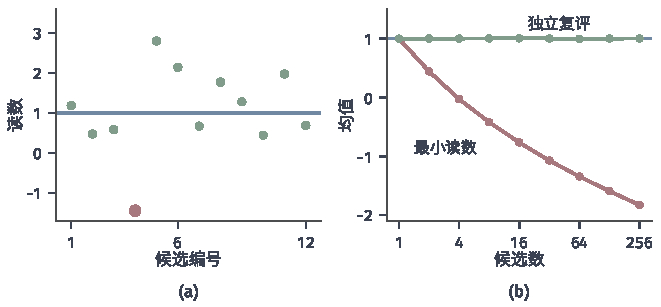
\includegraphics[width=112mm]{figures/05-optimization/05-stochastic-optimization/matplotlib/zo-selection/figure.pdf}
  \caption{含噪比较的选择偏差，真实值都是$1$（蓝线），噪声为标准正态。(a)$12$个候选的一次读数，红点是读数最低者，它并不比其他候选好。(b)红线是$K$个候选中最小读数的均值，随$K$增大而偏低；绿线是选定后独立复评的均值，始终等于真值。每点$10^5$次模拟。}
  \label{fig:zo-selection}
\end{BookInlineFigure}

\section{误差与查询成本}
\label{sec:zo-error-cost}

前面记下了各种误差的账，本节把它们合并。要解决的问题是：给定函数读数的总预算，误差由哪几部分构成，各种方法怎样比较，平滑问题上的结论又怎样回到原问题？比较时固定同一个评价预算，分开记录三种误差：平滑或差分偏差、随机方向误差和读数噪声。

\subsection{扰动尺度的取舍}
\label{sec:zo-tradeoff}

\paragraph{差商的U形曲线}
扰动太大，差商在量一段弯曲路径的平均坡度；扰动太小，一点噪声就被放大。这两股力量相反，总误差随尺度呈U形。

取均方误差分析。前向差商在二阶导有上界$L$时，偏差不超过$Lh/2$；中心差商在三阶导有上界$M$时，偏差不超过$Mh^2/6$。结合式~\eqref{eq:zo-quotient-noise}，独立噪声下的均方误差满足
\begin{equation}
 \mathrm{MSE}_{\mathrm{F}}(h)\leq\frac{L^2h^2}{4}+\frac{2\sigma^2}{h^2},\qquad
 \mathrm{MSE}_{\mathrm{C}}(h)\leq\frac{M^2h^4}{36}+\frac{\sigma^2}{2h^2}.
 \label{eq:zo-mse}
\end{equation}
第二项随$h$平方的倒数增长，这对独立的加性噪声是不可避免的。对两式右端关于$h$求导并令其为零，得到最优尺度
\begin{equation}
 h_{\mathrm{F}}=\Bigl(\frac{8\sigma^2}{L^2}\Bigr)^{1/4},\qquad
 h_{\mathrm{C}}=\Bigl(\frac{3\sigma}{M}\Bigr)^{1/3}.
 \label{eq:zo-optimal-h}
\end{equation}

继续用$\varphi(s)=s^2/2+s^3/6$，$s_0=1$，这里局部取$L=\varphi''(1)=2$，$M=1$，噪声$\sigma=0.01$。代入式~\eqref{eq:zo-optimal-h}，得到
\[
 h_{\mathrm{F}}\approx0.119,\qquad h_{\mathrm{C}}\approx0.311.
\]
最优点上的均方根误差分别约为$0.17$和$0.028$，如图~\ref{fig:zo-tradeoff}。差别不只在数值：中心差分可以用更大的$h$，这同时削弱了噪声放大，所以在噪声存在时收益比精确读数时更明显。

\begin{BookInlineFigure}
  \centering
  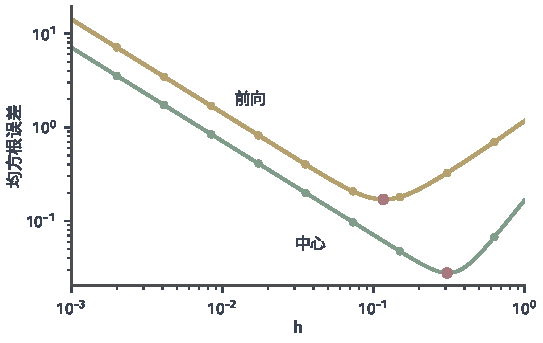
\includegraphics[width=92mm]{figures/05-optimization/05-stochastic-optimization/matplotlib/zo-tradeoff/figure.pdf}
  \caption{差商均方根误差随$h$的变化，$\varphi(s)=s^2/2+s^3/6$，$s_0=1$，独立噪声$\sigma=0.01$。黄线为前向差分，绿线为中心差分，曲线是偏差平方加方差的精确值，圆点是$2\times10^5$次模拟的结果，红点是各自的最小值。$h$小时两线斜率都是$-1$，$h$大时分别是$1$和$2$。}
  \label{fig:zo-tradeoff}
\end{BookInlineFigure}

\paragraph{迭代中的同一取舍}
在迭代算法中，平滑半径受同样的取舍支配，但记账的单位变了。定理~\ref{thm:zo-convex}的上界对$\delta$的依赖是$\alpha V+L\delta^2/2$，而$V$里的噪声项$\propto1/\delta^2$。

图~\ref{fig:zo-delta-u}用一个非二次的凸目标$f(\bm{x})=\sum_{i=1}^2(e^{x_i}-x_i-1)$做实验，解是原点，$f^\star=0$，算法跑固定轮数，噪声$\sigma=0.2$。$\delta$小的一侧，误差按$1/\delta^2$增长，来自噪声；$\delta$大的一侧，平滑目标的解偏离原点，误差快速上升。最好的$\delta$在$0.5$附近，目标差约$0.0026$，$\delta=0.02$和$\delta=4$时都超过$1$。

\begin{BookInlineFigure}
  \centering
  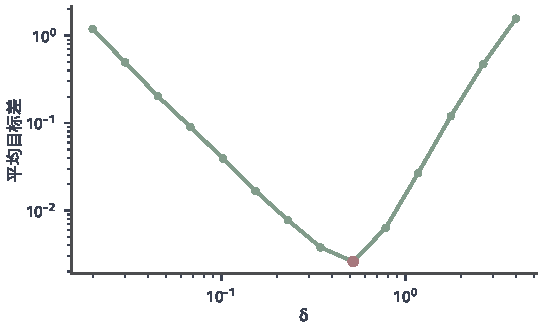
\includegraphics[width=92mm]{figures/05-optimization/05-stochastic-optimization/matplotlib/zo-delta-u/figure.pdf}
  \caption{双点方法在$f(\bm{x})=\sum_{i=1}^2(e^{x_i}-x_i-1)$上的平均目标差随$\delta$的变化，起点$(1,1)$，$\alpha=0.02$，$\sigma=0.2$，$T=3000$，取最后$500$步的平均，$200$次运行。左支由噪声放大主导，右支由平滑偏差主导，红点是扫描到的最小值。}
  \label{fig:zo-delta-u}
\end{BookInlineFigure}

\paragraph{共享样本时规律不同}
上面的$1/\delta^2$规律只适用于独立加性噪声。共享的Lipschitz样本下，差商的方差不随$\delta$增大而爆炸，$\delta$可以尽量取小，U形曲线的左支几乎消失。而指示函数样本的方差$\propto1/\delta$，左支依然存在，只是坡度减半。用哪个$\delta$要先确定噪声模型。

\subsection{维数与方向数}
\label{sec:zo-dimension}

“每轮只读两次”常被误解成成本与维数无关。上面的$\alpha\lesssim1/(nL)$已经说明，维数并没有消失，只是从每轮的读数次数转移到了步长上。

\paragraph{单轮比较}
表~\ref{tab:zo-moments}比较完整坐标差分和随机方向在单轮的成本与误差。这里的“方向波动”是读数精确时二次函数上的$\mathbb{E}\lVert\hat{\bm{g}}-\bm{g}\rVert_2^2$。

\begin{BookInlineTable}
  \centering
  \begin{tabular}{@{}llll@{}}
    \toprule
    方法 & 单轮读数 & 方向波动 & 独立噪声贡献\\
    \midrule
    中心坐标 & $2n$ & $0$ & $n\sigma^2/(2h^2)$\\
    单方向对称 & $2$ & $(n-1)\lVert\bm{g}\rVert_2^2$ & $n^2\sigma^2/(2\delta^2)$\\
    $m$方向对称 & $2m$ & $(n-1)\lVert\bm{g}\rVert_2^2/m$ & $n^2\sigma^2/(2m\delta^2)$\\
    $m$方向共用中心 & $m+1$ & 取决于函数 & $2n^2\sigma^2/(m\delta^2)$\\
    \bottomrule
  \end{tabular}
  \caption{一轮估计的成本与误差。$m=n$时，随机方向的噪声贡献与中心坐标差分相同，都是$n\sigma^2/(2\delta^2)$，读数次数也相同。}
  \label{tab:zo-moments}
\end{BookInlineTable}

\paragraph{相同预算下的结果}
图~\ref{fig:zo-dims}在$n=20$的二次目标上比较三种配置，步长按单轮二阶矩调节：坐标差分用$1/L$，$m$方向平均用$1/(L(1+(n-1)/m))$。横轴都是函数读数次数。读数精确时三条线基本平行，图(a)；读数含噪时停在几乎同一水平，图(b)。

\begin{BookInlineFigure}
  \centering
  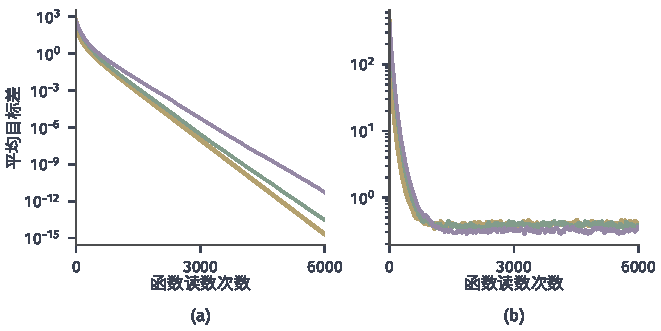
\includegraphics[width=112mm]{figures/05-optimization/05-stochastic-optimization/matplotlib/zo-dims/figure.pdf}
  \caption{$n=20$的二次目标，$\bm{H}$的对角元从$1$均匀到$9$，$h=\delta=0.1$，$30$次运行平均。黄线：中心坐标差分。绿线：$m=1$的随机方向。紫线：$m=5$的随机方向。(a)读数精确。(b)独立噪声$\sigma=0.1$。按读数次数计，三者的差别远小于“两次查询对$40$次查询”的字面差距。}
  \label{fig:zo-dims}
\end{BookInlineFigure}

这个实验的结论有范围。它说明在按读数计费、读数可独立提交的情形下，每轮少读并不等于总成本少。随机方向的优势在别处：可以在读完所有坐标之前就开始移动。梯度集中在少数方向时效果可能更好，但这取决于具体结构，本章没有相应的定理。反过来，如果读数可并行、每轮墙钟时间固定，完整差分反而可能更快。

\paragraph{方向平均与共用中心读数}
独立方向平均把方差除以$m$，这部分依赖独立性。为节省读数，有人让所有方向共用一次中心读数$y_0=f(\bm{x})+\zeta_0$，读数次数从$2m$降到$m+1$。这时
\[
 \hat{\bm{g}}=\frac{n}{\delta m}\sum_{j=1}^m(y_j-y_0)\bm{u}_j,
\]
噪声部分是$\tfrac{n}{\delta m}\sum_j(\zeta_j-\zeta_0)\bm{u}_j$。给定方向，$\zeta_0$对所有方向是同一个数，噪声不再独立，二阶矩是
\[
 \frac{n^2\sigma^2}{\delta^2m^2}\Bigl(m+\Bigl\lVert\sum_{j=1}^m\bm{u}_j\Bigr\rVert_2^2\Bigr).
\]
方向独立随机时$\mathbb{E}\lVert\sum_j\bm{u}_j\rVert_2^2=m$，总贡献是$2n^2\sigma^2/(m\delta^2)$，与每方向单独读中心点的情形相同。方向相关时，比如都偏向同一侧，第二项可以高达$m^2$。所以共用中心读数引入了相关性，必须单独计入。

坐标方向上这一点最清楚。前向坐标差分共用$f(\bm{x})$时，噪声的协方差是
\[
 \frac{\sigma^2}{h^2}\bigl(\bm{I}+\bm{1}\bm{1}^\top\bigr),
\]
它的特征值是$(n+1)\sigma^2/h^2$（对应方向$\bm{1}$）和$n-1$个$\sigma^2/h^2$。公共噪声把误差压到一个方向上，如图~\ref{fig:zo-cov}(a)，而中心差分的误差是各向同性的，如图(b)。

\begin{BookInlineFigure}
  \centering
  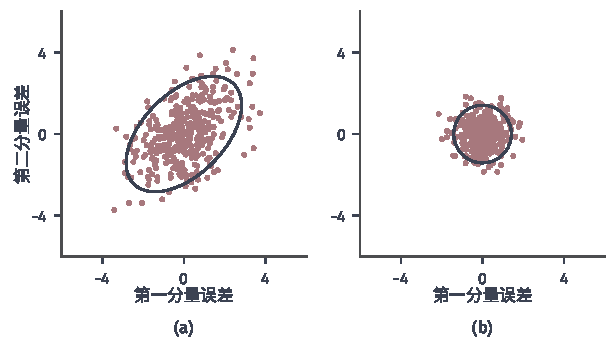
\includegraphics[width=104mm]{figures/05-optimization/05-stochastic-optimization/matplotlib/zo-cov/figure.pdf}
  \caption{$n=2$，$\sigma=h=0.1$时坐标差分的噪声误差。红点是$350$次模拟，黑色椭圆是两倍标准差的等概率线。(a)前向差分共用中心读数，协方差$\begin{bmatrix}2&1\\1&2\end{bmatrix}$，误差沿$(1,1)$方向拉长。(b)中心差分，协方差为$\tfrac12\bm{I}$。}
  \label{fig:zo-cov}
\end{BookInlineFigure}

\subsection{原目标的误差评价}
\label{sec:zo-original-error}

第~\ref{sec:zo-output}节的定理说的都是平滑目标。原来要解决的问题是最小化$f$，本小节补上这一步。

\paragraph{函数平滑误差}
设平滑目标$f_{\mathrm{s}}$与$f$处处至多相差$\gamma_f$，这个常数$\gamma_f$是\term{函数平滑误差}（function smoothing error）。由引理~\ref{lem:zo-smoothing-properties}，光滑函数的球平滑可取$\gamma_f=L\delta^2/2$，$G$-Lipschitz函数可取$\gamma_f=G\delta$。

\begin{theorem}[从平滑目标回到原目标]
\label{thm:zo-transfer}
设$\lvert f_{\mathrm{s}}-f\rvert\leq\gamma_f$，$\bm{x}^\star$是$f$的解，则对任意$\hat{\bm{x}}$，
\begin{equation}
 f(\hat{\bm{x}})-f^\star\leq f_{\mathrm{s}}(\hat{\bm{x}})-f_{\mathrm{s}}(\bm{x}^\star)+2\gamma_f.
 \label{eq:zo-function-transfer}
\end{equation}
若两者的梯度处处至多相差$\gamma_g$（按欧氏范数），则
\begin{equation}
 \lVert\nabla f(\hat{\bm{x}})\rVert_2^2\leq2\lVert\nabla f_{\mathrm{s}}(\hat{\bm{x}})\rVert_2^2+2\gamma_g^2.
 \label{eq:zo-gradient-transfer}
\end{equation}
\end{theorem}

\begin{proof}
由一致误差的假设，
\[
 f(\hat{\bm{x}})\leq f_{\mathrm{s}}(\hat{\bm{x}})+\gamma_f,\qquad f_{\mathrm{s}}(\bm{x}^\star)\leq f^\star+\gamma_f.
\]
两式相加移项得式~\eqref{eq:zo-function-transfer}。

由三角不等式，$\lVert\nabla f\rVert_2$不超过$\lVert\nabla f_{\mathrm{s}}\rVert_2+\gamma_g$，两边平方并用$(a+b)^2\leq2a^2+2b^2$，得式~\eqref{eq:zo-gradient-transfer}。
\end{proof}

式~\eqref{eq:zo-function-transfer}中的$2\gamma_f$在凸函数上可以省一半，因为$f\leq f^{\mathrm{B}}_{\delta}$。把定理~\ref{thm:zo-convex}代回，对光滑凸目标得到
\begin{equation}
 \mathbb{E}f(\bar{\bm{x}})-f^\star\leq\frac{R_0^2}{\alpha T}+\alpha V+L\delta^2.
 \label{eq:zo-convex-original}
\end{equation}
把定理~\ref{thm:zo-nonconvex}代回，取$\gamma_g=L\delta$，对光滑非凸目标得到
\begin{equation}
 \mathbb{E}\bigl\lVert\nabla f(\bm{x}^{(R)})\bigr\rVert_2^2\leq\frac{4\Delta_\delta}{\alpha T}+2L\alpha W+2L^2\delta^2.
 \label{eq:zo-nonconvex-original}
\end{equation}

\paragraph{平滑目标的解不是原目标的解}
这个换算的$\gamma_f$是不能省的。取$f(x)=\max\{x,-2x\}$，$n=1$，$\delta=1$，解是$x^\star=0$。$\lvert x\rvert<1$时，平滑目标的导数是
\[
 \bigl(f^{\mathrm{B}}_{\delta}\bigr)'(x)=\frac{f(x+1)-f(x-1)}{2}=\frac{3x-1}{2},
\]
零点在$x=1/3$，如图~\ref{fig:zo-asym}(a)。平滑目标的精确解带着原目标差$f(1/3)=1/3$。原目标两侧的斜率不对称，平均之后最低点向缓的一侧移动。这笔误差不是算法或噪声造成的，平滑的定义本身就带来了它。

\begin{BookInlineFigure}
  \centering
  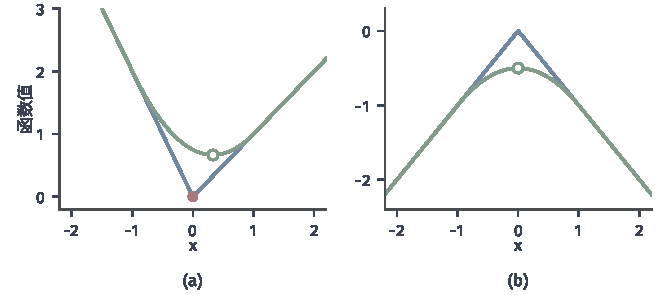
\includegraphics[width=112mm]{figures/05-optimization/05-stochastic-optimization/matplotlib/zo-asym/figure.pdf}
  \caption{平滑目标（绿）与原目标（蓝）的差别，$\delta=1$，一维区间平均。(a)$f(x)=\max\{x,-2x\}$，原解是红点$x=0$，平滑目标的解是空心点$x=1/3$，不在原解上。(b)$f(x)=-\lvert x\rvert$，平滑后在$x=0$处导数为零（空心点），而$x=0$是原函数的极大点。}
  \label{fig:zo-asym}
\end{BookInlineFigure}

\paragraph{原目标不光滑时要换驻点的概念}
式~\eqref{eq:zo-gradient-transfer}需要$\nabla f$存在且$\gamma_g$有限。原目标不可微时，平滑梯度小不能说明原目标梯度小。回到$f=\lvert x\rvert$，由$\bigl(f^{\mathrm{B}}_{\delta}\bigr)'(x)=x/\delta$，在$x=0.01\delta$处平滑导数只有$0.01$，而原函数在此处的导数是$1$。

平滑梯度小给出的是另一种结论。$f$是Lipschitz时，$\nabla f^{\mathrm{B}}_{\delta}(\bm{x})$是$\delta$邻域内各点梯度的平均，所以它小，说明邻域内的梯度有一个小的平均。这是Goldstein意义下的$\delta$驻点，比经典驻点弱。

这也不保证全局最优。图~\ref{fig:zo-asym}(b)的$f=-\lvert x\rvert$，平滑后$x=0$处导数为零，而$x=0$恰恰是原函数的极大点。更一般的多谷目标上，平滑可能磨掉一些浅谷，但没有定理保证平滑目标的驻点在全局最优点附近。

\subsection{函数评估总成本}
\label{sec:zo-total-cost}

\paragraph{成本的组成}
一次优化消耗的函数读数总数是
\begin{equation}
 Q=T\cdot m\cdot q\cdot r+Q_{\mathrm{eval}},
 \label{eq:zo-total-cost}
\end{equation}
其中$T$是迭代轮数，$m$是每轮方向数，$q$是每方向的查询次数，$r$是每个查询点的重复测量次数，$Q_{\mathrm{eval}}$是最终复评的开销。

取$T=200$，$m=2$，$q=2$，$r=3$，末了对$5$个候选各复评$20$次，代入式~\eqref{eq:zo-total-cost}，得到
\[
 Q=200\cdot2\cdot2\cdot3+5\cdot20=2500.
\]
重复测量$r$和扰动尺度$\delta$都能减小差商的噪声，但是方式不同：$r$把方差除以$r$，代价是读数翻$r$倍；增大$\delta$不需要额外读数，但引入偏差。

\paragraph{并行耗时与评估总量}
总量$Q$和实际等待时间是两个量。如果有$12$个并行的仿真槽，上例每轮的$12$次读数可同时提交，迭代部分需要$200$个批次，复评$100$次需要$9$个批次，总共$209$批。单线运行时就是$2500$次。比较算法时要说明用的是哪一个。并行时完整差分的劣势大大减小，甚至可能占优，因为它的每一轮都同时做完。

\paragraph{达到指定精度的成本}
下面把前面的上界解出来，得到达到精度$\varepsilon$所需的读数量级。$\sigma$是独立噪声的标准差。

读数精确且$f$是$L$-光滑凸函数时，由式~\eqref{eq:zo-convex-original}，$V=n^2L^2\delta^2/2$。取$\alpha=1/(4nL)$，上界是
\[
 \frac{4nLR_0^2}{T}+\Bigl(\frac{n}{8}+1\Bigr)L\delta^2.
\]
$\delta$可以任意小，只受浮点精度的限制。取$\delta^2\leq\varepsilon/((2+n/4)L)$，$T=8nLR_0^2/\varepsilon$，每轮两次读数，得到
\[
 Q=\frac{16\,nLR_0^2}{\varepsilon}.
\]
梯度下降需要$O(LR_0^2/\varepsilon)$次梯度，这里多出的正是因子$n$，同完整坐标差分的成本同阶。

独立噪声下，由式~\eqref{eq:zo-convex-original}和$V\approx n^2\sigma^2/(2\delta^2)$，把步长调到最优后上界约为
\[
 2R_0\sqrt{\frac{V}{T}}+L\delta^2=\frac{\sqrt{2}R_0n\sigma}{\delta\sqrt{T}}+L\delta^2.
\]
对$\delta$求最小，得$\delta\propto T^{-1/6}$，误差$\varepsilon\propto T^{-1/3}$，反解$T$得到$Q=O(LR_0^2n^2\sigma^2/\varepsilon^3)$。这里$\delta$必须随预算一起缩小，否则$L\delta^2$这项不消失。这是第~\ref{sec:zo-tradeoff}节U形曲线在迭代算法中的结果。

只有单点反馈且$f$是$G$-Lipschitz凸函数、$\lvert f\rvert\leq B$时，二阶矩是$n^2B^2/\delta^2$，平滑误差是$G\delta$。同样的累加分析给出误差约$R_0nB/(\delta\sqrt{T})+G\delta$，最优化$\delta$后$\varepsilon\propto T^{-1/4}$。

光滑非凸情形按式~\eqref{eq:zo-nonconvex-original}同样处理。精确读数时取足够小的$\delta$，$\alpha=1/(4nL)$，得$Q=O(nL\Delta/\varepsilon^2)$，这里$\Delta$是初始目标与下界之差。独立噪声时平衡$\delta$，得$\varepsilon^2\propto T^{-1/3}$，反解得表中的量级。

表~\ref{tab:zo-costs}汇总这些结果。

\begin{BookInlineTable}
  \centering
  \begin{tabular}{@{}lll@{}}
    \toprule
    反馈与正则性 & 估计器 & 读数量级\\
    \midrule
    精确，$L$-光滑凸 & 双点球面 & $nLR_0^2/\varepsilon$\\
    精确，$L$-光滑非凸 & 双点球面 & $nL\Delta/\varepsilon^2$\\
    独立噪声，$L$-光滑凸 & 双点球面 & $LR_0^2n^2\sigma^2/\varepsilon^3$\\
    独立噪声，$L$-光滑非凸 & 双点球面 & $L^3\Delta n^2\sigma^2/\varepsilon^6$\\
    单点，$G$-Lipschitz凸，$\lvert f\rvert\leq B$ & 单点球面 & $n^2R_0^2B^2G^2/\varepsilon^4$\\
    共享Lipschitz样本，凸 & 双点球面 & $n^2G^2R_0^2/\varepsilon^2$\\
    \bottomrule
  \end{tabular}
  \caption{本章简单估计器达到精度$\varepsilon$的读数量级，略去常数。凸问题的精度指目标差，非凸问题指$\lVert\nabla f\rVert_2\leq\varepsilon$；末行由$\lVert\hat{\bm{g}}\rVert_2\leq nG$的粗略界得到。这些都是上界，不是问题本身的下界。}
  \label{tab:zo-costs}
\end{BookInlineTable}

表的最后一行可以改进。利用球面上Lipschitz函数的集中不等式，双点估计的二阶矩能够改进到$O(nG^2)$，读数量级相应地变成$nG^2R_0^2/\varepsilon^2$。这一步的证明需要用到球面集中不等式，篇幅较长，读者可查阅Duchi等人及Shamir关于双点反馈的工作。它的含义是：共享样本下，配对的收益是把维数从平方降到一次方。

比较时要留意三件事。一是接口：表中的噪声列不能跨行混用，独立噪声的速率不适用于共享样本，反之亦然。二是度量：目标差和梯度范数的$\varepsilon$不是一回事。三是假设：更好的指数往往需要更强的光滑性和更复杂的估计器，不是换一个步长就能得到。

\section{本章小结}
\label{sec:zo-summary}

本章在只能读函数值的条件下回答了怎样构造方向、怎样迭代、最后得到什么保证。函数值反馈先要说清接口：精确值、加性噪声和样本函数是三种读数模型，单点与成对、独立噪声与共享样本是不同的读取条件，算法抽方向的随机性与读数的随机性分开记录。

局部方向有两种读法。有限差分以原梯度为对象：坐标差分需要$n+1$或$2n$次读数，随机方向差分和SPSA只需两次，但一条方向只有一条方向的信息，有限扰动下一般有偏，SPSA的坐标尺度乘以$\sqrt{n}$才是位移长度。随机平滑以平滑目标为对象：球平滑的恒等式~\eqref{eq:zo-ball-identity}和高斯平滑的恒等式~\eqref{eq:zo-gauss-identity}给出严格无偏的估计，单点估计受函数值大小影响，双点估计消去常数偏移。独立噪声让差商方差按$1/\delta^2$增长，共享样本是否改善取决于差值的波动。

把估计器代入迭代后，算法实际优化的目标由条件均值决定。步长受维数限制约为$1/(nL)$，扰动尺度决定平滑目标和噪声，缩小它要同时记入目标变化和方差增长。约束下要分清更新可行与查询可行，球形扰动可用收缩集合，高斯扰动有无界支撑。输出按问题选择平均点或随机返回点，预算耗尽、读数不变和驻点保证是不同的停止依据，含噪比较需要独立复评。

按读数计费时，两次查询并不代表成本与维数无关，因子$n$转移到了步长上。平滑目标上的结论要加上平滑误差才是原目标的结论，原目标不光滑时平滑梯度小只是较弱的驻点概念，也不保证全局最优。选择方法时，先看接口：能读坐标且读数便宜就用差分；扰动必须同时施加时用SPSA；只有单点反馈时用单点估计；能共享样本时优先双点估计并尽量取小$\delta$。

高斯平滑的恒等式也可以看作：把$\bm{x}$当作高斯搜索分布的均值，这个估计描述均值移动时平均目标的变化。第~\ref{chap:random-search}章继续讨论怎样更新搜索分布和种群，那里的方法不都等同于本章的零阶梯度下降。


\chapter{随机搜索}
\label{chap:random-search}

要安排一批车辆的出发顺序，或者调一台模拟程序的几个开关和旋钮，每试一组方案，都只能得到一个代价数字。没有梯度，顺序和开关也谈不上求导；代价随方案的变化还可能高低起伏，朝眼前更好的方向走几步就停在一个局部低谷里。这时能做的，是决定下一批试哪些方案，以及怎样利用已经试过的结果。

第~\ref{chap:zeroth-order-optimization}章用函数值构造局部方向，仍然沿着一条路径向下走。本章换一种组织方式：不估计方向，而是管理候选。把这种方式统称为\term{随机搜索}（random search）：用随机提议产生候选，用评价结果决定保留什么，再由保留下来的信息安排后续的提议。

下面先固定问题，看清局部改善为什么会停。然后依次讨论四类方法，它们的差别在于保存什么、怎样更新：模拟退火只保存一个状态，靠接受规则决定要不要走；演化策略保存一个高斯分布，靠选择结果调整它的中心和形状；遗传算法保存一个种群，靠编码上的交叉和变异重组已有候选；粒子群让每个候选带着速度和记忆移动。

后三节处理所有方法共有的问题：候选不可行时怎么办，读数有噪声时最好记录还能不能信，结果应当怎样报告。全章反复用到两个小例子，一个是七个状态的双谷代价，一个是二维多峰函数，手算的步骤都在这些例子上进行。

\section{搜索问题}
\label{sec:rs-problem}

只能评价候选时，搜索到底在面对什么？先把目标、允许的候选和一次评价的回报固定下来，再看局部改善为什么会停滞。

\paragraph{目标、候选和一次评价}
全章考虑的问题写成
\begin{equation}
 \min_{\bm{x}\in\bm{C}}f(\bm{x}),
 \label{eq:rs-problem}
\end{equation}
其中$\bm{C}$是允许的候选集合，$f$是待最小化的代价，$f^\star$和$\bm{x}^\star$是最优值和最优解。$\bm{C}$可以是$\mathbb{R}^n$的一块区域，也可以是有限集合，比如所有长度为$n$的0--1串，或者$n$个元素的所有排列。

算法与问题之间只有一种接触方式：提交一个候选$\bm{x}$，收到一个数。这叫一次\term{评价}（evaluation）。收到的数不告诉我们$f$在别处的取值，也不带梯度或曲率。全章把预算记作$B$，表示允许的评价总次数；字母$T$留给后面的温度。

\paragraph{局部改善为什么会停}
看一个最小的例子。状态集合是$\{1,2,\ldots,7\}$，每个状态只与左右相邻的状态相连，代价是
\begin{equation}
 \bigl(f(1),f(2),\ldots,f(7)\bigr)=(3,\,1,\,3,\,5,\,2,\,0,\,2).
 \label{eq:rs-double-valley}
\end{equation}
全局最小在$x=6$，代价为$0$；$x=2$是另一个低谷，代价为$1$。两个低谷之间隔着代价为$5$的$x=4$。

规则“只走向更低的邻居”从$x=3$出发，下一步到$x=2$。在$x=2$，两个邻居的代价都是$3$，都比当前高，于是永远停在这里。从$1,2,3$出发都停在$x=2$，从$4,5,6,7$出发才能到达$x=6$。七个状态里有三个起点拿不到最优解，而算法在$x=2$上收不到任何“还有更好的地方”的信号。这就是图~\ref{fig:rs-two-landscapes}(a)。

连续变量也一样。考虑二维的Rastrigin函数
\begin{equation}
 f(\bm{x})=20+\sum_{i=1}^{2}\bigl(x_i^2-10\cos(2\pi x_i)\bigr).
 \label{eq:rs-rastrigin}
\end{equation}
全局最小在原点，$f^\star=0$。余弦项在每个整数点附近挖出一个小坑，在$[-5.12,5.12]^2$内共有$11^2=121$个局部极小点。

图~\ref{fig:rs-two-landscapes}(b)从四个起点运行梯度下降，每条路径都很快落进离起点最近的小坑。例如从$(-2.3,2.6)$出发，终点约为$(-1.99,2.98)$，那里的代价约为$12.9$。梯度下降在那里做的是对的事情，梯度也确实趋于零，只是这个驻点离全局最小还很远。

\begin{BookInlineFigure}
 \centering
 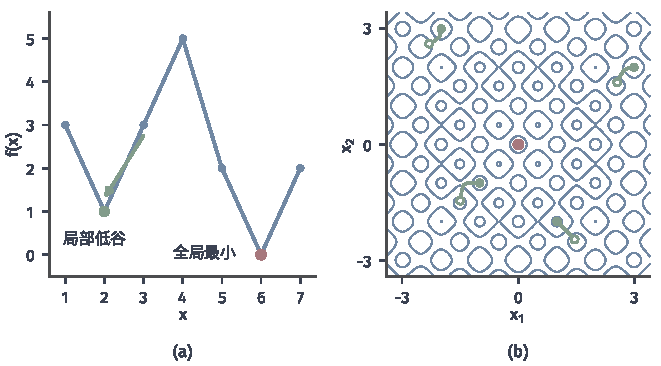
\includegraphics[width=112mm]{figures/05-optimization/05-stochastic-optimization/matplotlib/rs-two-landscapes/figure.pdf}
 \caption{两个多谷的代价。(a)七状态双谷代价~\eqref{eq:rs-double-valley}，绿色箭头是从$x=3$出发的下降，绿点是停止处，红点是全局最小。(b)二维Rastrigin函数~\eqref{eq:rs-rastrigin}的等高线（$f=8,24,40$），绿色曲线是从四个空心起点运行的梯度下降，它们都停在邻近的局部极小点（绿色实心点），红点是全局最小点。}
 \label{fig:rs-two-landscapes}
\end{BookInlineFigure}

要越过这样的障碍，算法必须做一些眼前并不划算的事：接受更差的候选，或者同时在多个地方试探。本章各方法的差别就在这里。

\paragraph{三个不同的数}
讨论算法时要分清三个数，它们经常被混为一谈。第一个是\textbf{真实目标值}$f(\bm{x})$，这是问题真正关心的量。

第二个是\textbf{读数}。评价可能含有噪声，这时收到的是
\begin{equation}
 \tilde f(\bm{x})=f(\bm{x})+\varepsilon,
 \label{eq:rs-reading}
\end{equation}
其中$\varepsilon$是这一次评价的误差。无噪声时$\tilde f=f$。第~\ref{sec:rs-noise}节之前都设无噪声。

第三个是\textbf{历史最好记录}。算法运行到第$t$次评价时，把已见的可行候选中读数最低的那个单独存下来：
\begin{equation}
 \begin{gathered}
 \bm{x}_{\mathrm{best}}^{(t)}\in\argmin\bigl\{\tilde f(\bm{x}^{(s)}):s\leq t,\ \bm{x}^{(s)}\in\bm{C}\bigr\},\\
 f_{\mathrm{best}}^{(t)}=\min_{s\leq t,\,\bm{x}^{(s)}\in\bm{C}}\tilde f(\bm{x}^{(s)}).
 \end{gathered}
 \label{eq:rs-best-record}
\end{equation}
无噪声时$f_{\mathrm{best}}^{(t)}$是真实值，而且随$t$不增。有噪声时它只是“最幸运的读数”，第~\ref{sec:rs-noise}节专门讨论这个差别。

\subsection{搜索空间}
\label{sec:rs-space}

同一个问题有不同的方式描述“从这个候选能走到哪里”。这一小节的问题是：候选的表示和移动方式怎样决定了搜索能到达什么地方？

\paragraph{三种候选，三种移动}
连续参数$\bm{x}\in\mathbb{R}^n$上最常用的移动是扰动$\bm{x}+\sigma\bm{z}$，其中$\bm{z}$是随机向量，$\sigma>0$控制尺度。一步可以到达的候选充满$\bm{x}$周围的一片区域。

二进制串$\bm{b}\in\{0,1\}^n$上的基本移动是翻位：改变一位。长度为$n$的串恰有$n$个翻位邻居，任何两个串之间相差几位，就至少需要几次翻位。

排列是把$n$个元素排成一列，$n!$种排法对应$n!$个候选。基本移动是交换两个位置上的元素。图~\ref{fig:rs-moves}把三种移动画在一起。

\begin{BookInlineFigure}
 \centering
 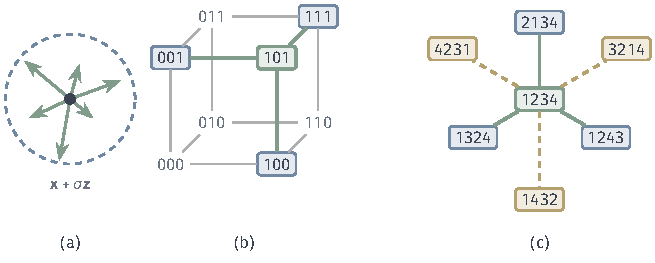
\includegraphics[width=111mm]{figures/05-optimization/05-stochastic-optimization/tikz/rs-moves/figure.pdf}
 \caption{三种候选上的移动，绿色表示当前候选及其一步移动。(a)连续参数的扰动，虚线圆表示尺度$\sigma$的量级。(b)三位二进制串构成立方体，蓝框是$101$的三个翻位邻居。(c)排列$1234$的邻居，蓝框是相邻交换，黄框和虚线是不相邻位置的交换。}
 \label{fig:rs-moves}
\end{BookInlineFigure}

把“一步能到达的候选”记为\term{邻域}（neighborhood）$\bm{N}(\bm{x})\subset\bm{C}$。邻域决定了一张图：候选是顶点，$\bm{y}\in\bm{N}(\bm{x})$就连一条边。局部低谷、爬坡路径都是相对这张图而言的，换一个邻域，低谷可能就不存在了。

\paragraph{编码要保留原问题的含义}
候选的表示必须让移动后的结果仍然有意义。例如选择问题用0--1串，第$i$位表示第$i$件物品选或不选，翻一位正是“多拿或少拿一件”，含义清楚。

把一个$0$到$15$的整数写成四位二进制，翻最高位会使整数变化$8$，翻最低位只变化$1$。从$7=0111$到相邻的$8=1000$要同时翻四位，数值上的近邻在编码上反而很远。这种表示下，翻位邻域与“数值接近”不是一回事，邻域的设计要先问清楚这一点。

\paragraph{相邻交换与任意交换}
用同一个问题比较两种邻域。平面上五个城市$A(1,4)$、$B(2,4)$、$C(3,5)$、$D(2,5)$、$E(5,0)$，距离取坐标差绝对值之和，一个访问顺序的代价是相邻两城距离之和，不返回起点。当前顺序$ABECD$的代价是
\[
 1+7+7+1=16.
\]
这条路线在中途绕向远处的$E$，然后折返，见图~\ref{fig:rs-swap-tour}(a)。

相邻交换只调换相邻的两个位置，$ABECD$的四个邻居的代价是
\[
 BAECD:17,\qquad AEBCD:18,\qquad ABCED:18,\qquad ABEDC:17.
\]
都比$16$高，所以$ABECD$是相邻交换下的局部低谷。

任意交换允许调换任何两个位置。交换$E$和$D$得到$ABDCE$，代价是
\[
 1+1+1+7=10,
\]
一步就到了五城问题的最优解，见图~\ref{fig:rs-swap-tour}(b)。

相邻交换也能到达最优解，只是要先爬坡：$ABECD\to ABCED\to ABCDE\to ABDCE$，代价依次是
\[
 16\ \to\ 18\ \to\ 12\ \to\ 10.
\]
这条路要先翻过高度为$2$的坎。同一对候选，在一种邻域下一步可达，在另一种邻域下隔着障碍。

\begin{BookInlineFigure}
 \centering
 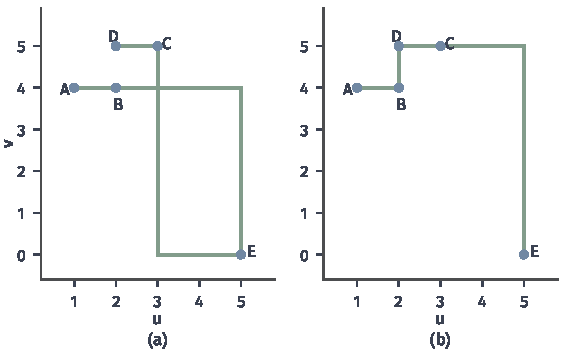
\includegraphics[width=96mm]{figures/05-optimization/05-stochastic-optimization/matplotlib/rs-swap-tour/figure.pdf}
 \caption{五城访问顺序，绿线按坐标差绝对值之和的路线画出，$u,v$是城市的横纵坐标。(a)顺序$ABECD$，长度$16$，四种相邻交换都使长度变大。(b)交换不相邻的$E$和$D$得到$ABDCE$，长度$10$。}
 \label{fig:rs-swap-tour}
\end{BookInlineFigure}

邻域并不是越大越好。五个位置时，相邻交换的邻居有$4$个，任意交换的有$10$个。任意两个排列之间，相邻交换至多需要$10$步，任意交换至多需要$4$步。

表~\ref{tab:rs-swap-neighborhood}列出这个比较。邻域大，一步能跳得远，图的直径小；代价是随机抽一个邻居时，抽到好邻居的机会被稀释，要穷举全部邻居时评价次数也更多。邻域的大小和移动尺度是算法设计中要专门决定的量，它与后面的接受规则彼此独立。

\begin{BookInlineTable}
 \centering
 \caption{$n$个元素的排列上两种交换邻域的比较，括号内是$n=5$的值。}
 \label{tab:rs-swap-neighborhood}
 \begin{tabular}{lll}
  \toprule
  & 相邻交换 & 任意交换 \\
  \midrule
  邻居个数 & $n-1$（$4$） & $n(n-1)/2$（$10$） \\
  任两排列间的最多步数 & $n(n-1)/2$（$10$） & $n-1$（$4$） \\
  是否能到达所有排列 & 能 & 能 \\
  一次移动改变的位置关系 & 小 & 可能很大 \\
  \bottomrule
 \end{tabular}
\end{BookInlineTable}

\subsection{搜索状态}
\label{sec:rs-state}

邻域回答“能走到哪里”。接下来的问题是：两次评价之间，算法手里究竟保存着什么？后面四类方法在这一点上差别最大，先把它们放在一起对比。

\paragraph{四种需要区分的对象}
\textbf{当前候选}是算法下一步移动的出发点，模拟退火就只维护这一个点。\textbf{群体成员}是同时维护的多个候选，遗传算法和粒子群属于这一类，粒子还各自带着速度。

\textbf{搜索分布参数}不是候选，而是描述“下一批候选从哪里抽”的量，例如高斯分布的中心和协方差。中心$\bm{m}$本身可能从未被评价过。\textbf{历史最好记录}是式~\eqref{eq:rs-best-record}定义的结果，它只被写入，不参与移动，除非某种算法特意使用它。

图~\ref{fig:rs-carriers}画出前三种状态，空心圆是各自的历史最好记录。表~\ref{tab:rs-state}比较它们带着什么信息。

\begin{BookInlineFigure}
 \centering
 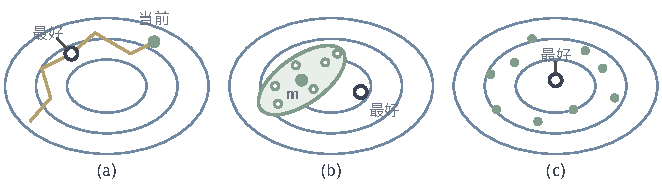
\includegraphics[width=112mm]{figures/05-optimization/05-stochastic-optimization/tikz/rs-carriers/figure.pdf}
 \caption{三种搜索状态，蓝线是目标等高线，空心圆是单独保存的历史最好记录。(a)单个当前候选（绿点）及其走过的路径（黄线），当前点可以比历史最好差。(b)搜索分布，绿点是中心$\bm{m}$，椭圆是分布的形状，空心小圆是抽到的后代，最好记录可能在椭圆外。(c)候选群体。}
 \label{fig:rs-carriers}
\end{BookInlineFigure}

\begin{BookInlineTable}
 \centering
 \caption{搜索状态承载的信息。}
 \label{tab:rs-state}
 \begin{tabular}{lll}
  \toprule
  状态 & 记住什么 & 下一批候选从哪里来 \\
  \midrule
  单个候选 & 一个点 & 这个点的邻域 \\
  搜索分布 & 中心、尺度、形状 & 从分布抽样 \\
  候选群体 & 多个点及其评价 & 成员的组合与变动 \\
  \bottomrule
 \end{tabular}
\end{BookInlineTable}

\paragraph{为什么要单独保存最好记录}
后面会看到，模拟退火有时接受更差的候选，整代替换的算法会把上一代全部丢弃。当前状态的代价因此可以上升，算法停止时手里的当前点可能比中途见过的某个点差很多。

保存记录的代价只是多存一个点。它不影响搜索的走向，却保证无噪声时交出的结果不差于任何已见的可行候选。所以无论采用什么算法，完整流程都要写上这一步。

\paragraph{与函数值方向估计的分工}
第~\ref{chap:zeroth-order-optimization}章也只用函数值：在当前点附近做差分或随机方向试探，组成梯度的估计$\hat{\bm{g}}^{(t)}$，再走一步：
\[
 \bm{x}^{(t+1)}=\bm{x}^{(t)}-\alpha^{(t)}\hat{\bm{g}}^{(t)}.
\]
它的主要对象是一个点和一个方向，分析用的是局部光滑性。

本章的主要对象是候选和选择，通常只用比较结果，也不要求$f$有导数，排列、开关这样的离散候选上根本谈不上方向。两者也有重合之处：后面第~\ref{sec:rs-es}节的高斯搜索分布，其均值的更新量可以看成平滑目标的梯度估计，这样的方法同时属于两种视角。

\section{模拟退火}
\label{sec:rs-sa}

上一节的双谷问题里，只走向更低邻居的规则停在$x=2$。这就需要回答：只维护一个状态，怎样让它有机会翻过障碍，又不至于一直乱走？\term{模拟退火}（simulated annealing，SA）的回答是：偶尔接受更差的候选，并让这种“偶尔”随时间变少。

用下山来想。一个人站在低谷里，四周都是上坡。如果他绝不上坡，就永远出不去；如果他毫不在乎坡度，就只是在地图上乱逛。合理的做法是：小坡常常愿意爬，大坡很少愿意爬，而且越到后面越不愿意爬。控制这份“愿意”的量就是温度。这个比喻到此为止：人站在山上看得到四周的坡，算法只知道它提议的那一点的代价。

\subsection{提议与接受}
\label{sec:rs-sa-accept}

一步退火由提议和接受组成。这一小节的问题是：接受规则应当怎样写，固定温度下它长期会把状态带到哪里？

\paragraph{主要思想}
一步分两半。先\textbf{提议}：从当前状态$\bm{x}$按分布$q(\bm{x},\cdot)$抽一个候选$\bm{y}$。这里设提议是对称的，即对任意$\bm{x},\bm{y}$，有$q(\bm{x},\bm{y})=q(\bm{y},\bm{x})$。

再\textbf{接受}：给定温度$T>0$，计算
\begin{equation}
 a_T(\bm{x},\bm{y})=\min\Bigl\{1,\ \exp\Bigl(-\frac{f(\bm{y})-f(\bm{x})}{T}\Bigr)\Bigr\},
 \label{eq:rs-metropolis}
\end{equation}
以概率$a_T(\bm{x},\bm{y})$移动到$\bm{y}$，否则留在$\bm{x}$。

下降或持平的提议一定被接受，上升的提议按上升量指数衰减的概率被接受。图~\ref{fig:rs-sa-acceptance}(a)画出这个函数：$T$大时曲线平缓，上坡也常被接受；$T\to0$时规则退回到只接受不上升的移动。

在双谷代价~\eqref{eq:rs-double-valley}上取$T=2$，算一次下降和一次上升。从$x=3$提议$y=2$，代价差是$-2$，接受概率为$1$。反过来，从$x=2$提议$y=3$，代价差是$+2$，接受概率为
\[
 \exp(-2/2)=\mathrm{e}^{-1}\approx0.368.
\]

上坡的代价差要除以温度才有意义。把$f$整体乘以$10$，同时把$T$乘以$10$，接受概率完全不变。所以温度的单位就是代价的单位，选温度必须看代价的尺度。

\paragraph{固定温度下的长期分布}
温度固定时，状态序列是一个马尔可夫链：下一个状态的分布只取决于当前状态。对$\bm{y}\neq\bm{x}$，一步转移的概率是
\begin{equation}
 P_T(\bm{x},\bm{y})=q(\bm{x},\bm{y})\,a_T(\bm{x},\bm{y}),
 \label{eq:rs-sa-transition}
\end{equation}
被拒绝的概率加到$P_T(\bm{x},\bm{x})$上。这个规则与下面的\term{Gibbs分布}（Gibbs distribution）紧密相关。在有限状态集合$\bm{C}$上定义
\begin{equation}
 \pi_T(\bm{x})=\frac{\exp(-f(\bm{x})/T)}{Z_T},\qquad
 Z_T=\sum_{\bm{u}\in\bm{C}}\exp(-f(\bm{u})/T).
 \label{eq:rs-gibbs}
\end{equation}
代价越低，权重越大。

\begin{theorem}[细致平衡]
\label{thm:rs-detailed-balance}
设$\bm{C}$有限，$q$对称，$T>0$。则对任意$\bm{x},\bm{y}\in\bm{C}$，
\begin{equation}
 \pi_T(\bm{x})P_T(\bm{x},\bm{y})=\pi_T(\bm{y})P_T(\bm{y},\bm{x}),
 \label{eq:rs-detailed-balance}
\end{equation}
因此$\pi_T$是转移矩阵$\bm{P}_T$的平稳分布。
\end{theorem}

\begin{proof}
$\bm{x}=\bm{y}$时两边相同。设$\bm{x}\neq\bm{y}$，不妨设$f(\bm{y})\geq f(\bm{x})$，否则交换两者的名字。这时从$\bm{y}$到$\bm{x}$是下降，$a_T(\bm{y},\bm{x})=1$，于是右边是
\[
 \pi_T(\bm{y})P_T(\bm{y},\bm{x})=\frac{\exp(-f(\bm{y})/T)}{Z_T}\,q(\bm{y},\bm{x}).
\]

从$\bm{x}$到$\bm{y}$是上升，代入式~\eqref{eq:rs-metropolis}，左边是
\[
 \begin{aligned}
 \pi_T(\bm{x})P_T(\bm{x},\bm{y})
 &=\frac{\exp(-f(\bm{x})/T)}{Z_T}\,q(\bm{x},\bm{y})\exp\Bigl(-\frac{f(\bm{y})-f(\bm{x})}{T}\Bigr)\\
 &=\frac{\exp(-f(\bm{y})/T)}{Z_T}\,q(\bm{x},\bm{y}).
 \end{aligned}
\]
由$q$的对称性，两边相等。

对式~\eqref{eq:rs-detailed-balance}关于$\bm{x}$求和，转移概率对第二个变量求和为$1$，于是
\[
 \sum_{\bm{x}}\pi_T(\bm{x})P_T(\bm{x},\bm{y})=\pi_T(\bm{y}),
\]
这正是平稳性。
\end{proof}

平稳分布存在不等于状态序列一定趋向它。若提议图连通，并且链不被周期卡住（例如某些状态有正的停留概率），状态的分布才从任何起点收敛到$\pi_T$。这一收敛结论的证明用到有限马尔可夫链的基本定理，可参考\BookChapterRef{chap:discrete-time-stochastic-processes}{卷九第3章“离散时间随机过程”}。

图~\ref{fig:rs-sa-acceptance}(b)是双谷问题的$\pi_T$。$T=2$时六号状态的概率约为$0.348$，二号状态约为$0.211$，高处的状态也有不小的份额。$T=0.5$时六号状态约为$0.850$，二号状态约为$0.115$。

\begin{BookInlineFigure}
 \centering
 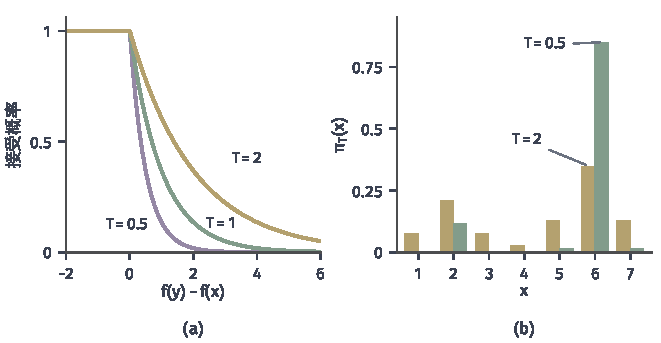
\includegraphics[width=112mm]{figures/05-optimization/05-stochastic-optimization/matplotlib/rs-sa-acceptance/figure.pdf}
 \caption{接受规则与长期分布。(a)接受概率~\eqref{eq:rs-metropolis}作为代价差的函数。(b)双谷代价~\eqref{eq:rs-double-valley}的Gibbs分布，黄色柱为$T=2$，绿色柱为$T=0.5$，温度越低，概率越集中在代价低的状态。}
 \label{fig:rs-sa-acceptance}
\end{BookInlineFigure}

温度趋于零时，$\pi_T$集中到全局最小点上。设$\bm{S}^\star$是全局最小点的集合，对任一非全局最小点$\bm{x}$和$\bm{x}^\star\in\bm{S}^\star$，比值
\[
 \frac{\pi_T(\bm{x})}{\pi_T(\bm{x}^\star)}=\exp\Bigl(-\frac{f(\bm{x})-f^\star}{T}\Bigr)\to0\qquad(T\to0^+).
\]
状态有限，所以$\pi_T(\bm{S}^\star)\to1$。这就是降温的动机：低温时的长期分布几乎全在最优解上。

问题在于“长期”。温度越低，翻越障碍越慢，走到长期分布所需的时间越长。第~\ref{sec:rs-sa-barrier}节把这件事说清楚。

\paragraph{提议不对称会怎样}
证明的最后一步用了$q$的对称性。提议不对称时，平衡关系就不再成立。看两个状态、代价相同的情形，$\pi_T=(1/2,1/2)$。

设从状态$1$总是提议$2$，而从状态$2$以$1/2$的概率提议$1$，以$1/2$的概率提议自身。代价相同，接受概率都是$1$。两状态的平稳条件是$\pi(1)\cdot1=\pi(2)\cdot\tfrac12$，于是
\[
 \pi=\Bigl(\frac13,\frac23\Bigr)\neq\Bigl(\frac12,\frac12\Bigr).
\]

要恢复目标分布，需要把提议比例放进接受概率：
\begin{equation}
 a_T(\bm{x},\bm{y})=\min\Bigl\{1,\ \exp\Bigl(-\frac{f(\bm{y})-f(\bm{x})}{T}\Bigr)\frac{q(\bm{y},\bm{x})}{q(\bm{x},\bm{y})}\Bigr\}.
 \label{eq:rs-hastings}
\end{equation}
上面的例子里，$a(1,2)=1/2$，$a(2,1)=1$，两个方向的流量都是$\pi(\cdot)\cdot\tfrac12$，$(1/2,1/2)$重新平稳。这个修正的一般讨论可参考\BookChapterRef{chap:random-sampling-integration}{卷七第14章“随机采样与积分计算”}。

\needspace{6\baselineskip}
\paragraph{变量}
下面在双谷代价上手算几步。要维护的量是：
\begin{itemize}
 \item $x^{(t)}$：当前状态，$f(x^{(t)})$是它的代价；
 \item $T^{(t)}>0$：第$t$步的温度；
 \item $x_{\mathrm{best}}$，$f_{\mathrm{best}}$：历史最好记录。
\end{itemize}

\paragraph{初始化}
选起点和初始温度，把起点记为最好记录。例中从局部低谷出发，温度每步乘以$0.9$：
\[
 x^{(0)}=2,\qquad T^{(0)}=2,\qquad T^{(t)}=2\times0.9^{t},\qquad f_{\mathrm{best}}=1.
\]
提议是等概率选左或右，超出范围时提议留在原地。

\paragraph{每轮更新}
第$t$轮依次执行以下步骤，直到用完预算。下面每一轮的提议方向和均匀随机数$u$都是事先列好的，以便逐步核对。

\begin{enumerate}
 \item 从$q(x^{(t)},\cdot)$抽候选$y$，评价$f(y)$。例中第$0$轮提议$y=1$，$f(y)=3$。
 \item 由式~\eqref{eq:rs-metropolis}计算接受概率。例中第$0$轮代价差是$2$，$T^{(0)}=2$，接受概率为$0.368$。
 \item 抽$u\sim\mathrm{U}(0,1)$，若$u<a$，令$x^{(t+1)}=y$，否则$x^{(t+1)}=x^{(t)}$。例中第$0$轮$u=0.71$，拒绝，状态仍为$2$。
 \item 若$y$可行且$f(y)<f_{\mathrm{best}}$，更新最好记录。例中第$0$轮不更新。
\end{enumerate}

表~\ref{tab:rs-sa-hand}列出前六轮。第$1$、$2$轮两次上坡都被接受，状态爬到垒顶$x=4$，代价是$5$，比记录差很多；接着第$3$、$4$轮是下坡，必然接受，第$4$轮到达$x=6$，最好记录更新为$0$。第$5$轮提议上坡到$x=7$，被拒绝。

\begin{BookInlineTable}
 \centering
 \caption{双谷代价上的前六轮，$a$是接受概率，$u$是列好的随机数。}
 \label{tab:rs-sa-hand}
 \begin{tabular}{rrrrrrrr}
  \toprule
  $t$ & $T^{(t)}$ & $x^{(t)}$ & $y$ & $f(y)-f(x^{(t)})$ & $a$ & $u$ & $f_{\mathrm{best}}$ \\
  \midrule
  $0$ & $2.000$ & $2$ & $1$ & $+2$ & $0.368$ & $0.71$ & $1$ \\
  $1$ & $1.800$ & $2$ & $3$ & $+2$ & $0.329$ & $0.25$ & $1$ \\
  $2$ & $1.620$ & $3$ & $4$ & $+2$ & $0.291$ & $0.18$ & $1$ \\
  $3$ & $1.458$ & $4$ & $5$ & $-3$ & $1$ & --- & $1$ \\
  $4$ & $1.312$ & $5$ & $6$ & $-2$ & $1$ & --- & $0$ \\
  $5$ & $1.181$ & $6$ & $7$ & $+2$ & $0.184$ & $0.62$ & $0$ \\
  \bottomrule
 \end{tabular}
\end{BookInlineTable}

最终得到$x_{\mathrm{best}}=6$，$f_{\mathrm{best}}=0$。这是特意挑选的一条幸运路径，连续爬坡两次的概率并不大，真实的成功机会要由下面的整体计算回答。

这个例子也说明了两条轨迹的区别：当前状态在第$2$轮爬到了代价$5$，比出发时差得多，而记录始终不变差。

\subsection{温度与能垒}
\label{sec:rs-sa-barrier}

温度要降到多慢，才能保证最终找到全局最小？这一小节回答这个问题，也要说明这个答案能用到什么程度。

\paragraph{能垒}
在双谷问题中，从$x=2$到代价更低的$x=6$，必须经过$x=4$。路径上的最高代价是$5$，比出发点高$4$。这个高度刻画了离开这个低谷的困难。

一般地，给定提议图和一个不是全局最小的局部低谷$\bm{x}$，考虑从$\bm{x}$到所有代价严格更低的状态的路径。路径$\bm{x}=\bm{w}_0,\bm{w}_1,\ldots,\bm{w}_k$沿提议图的边走，$f(\bm{w}_k)<f(\bm{x})$。定义\term{能垒}（energy barrier）为
\begin{equation}
 d(\bm{x})=\min_{\text{路径}}\ \max_{0\leq j\leq k}\bigl(f(\bm{w}_j)-f(\bm{x})\bigr),
 \label{eq:rs-barrier}
\end{equation}
即在所有出路中，选最省力的一条，所要爬的最大高度。全部非全局低谷的能垒中最大的一个记为$d^\star$。

双谷问题只有一个非全局低谷$x=2$。向左走不通，向右必须经过$x=4$，所以
\[
 d(2)=5-1=4,\qquad d^\star=4.
\]
图~\ref{fig:rs-barrier-depth}标出这个高度。注意能垒不等于单步的代价差：$x=2$的邻居只比它高$2$，真正要爬的是连续两步累计的$4$。

\begin{BookInlineFigure}
 \centering
 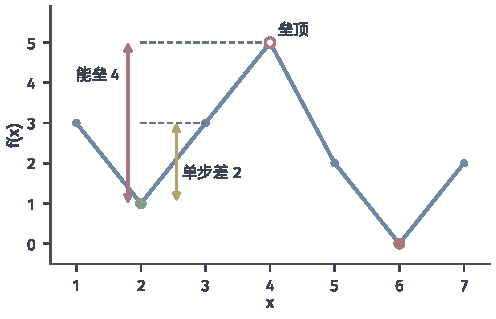
\includegraphics[width=84mm]{figures/05-optimization/05-stochastic-optimization/matplotlib/rs-barrier-depth/figure.pdf}
 \caption{双谷代价的能垒。绿点是非全局低谷$x=2$，空心红点是通往全局最小（红色实心点）必经的垒顶$x=4$。红色双箭头是能垒$d(2)=4$，黄色双箭头是一步上坡的代价差$2$。}
 \label{fig:rs-barrier-depth}
\end{BookInlineFigure}

\paragraph{对数降温的条件}
先看量级。温度为$T$时，翻过能垒$d$的那条路径大约要付出$\exp(-d/T)$的概率，所以大约要等$\exp(d/T)$步才能出去一次。$T=1$时$\mathrm{e}^4\approx55$步，$T=0.25$时已经约有$8.9\times10^{6}$步。

要让出去的机会永远不会用完，把每一步的逃逸机会加起来应当发散：
\[
 \sum_{t}\exp(-d^\star/T^{(t)})=\infty.
\]
取\term{对数降温}（logarithmic cooling）$T^{(t)}=c/\log(t+2)$，有$\exp(-d^\star/T^{(t)})=(t+2)^{-d^\star/c}$，这个级数在$c\geq d^\star$时发散，在$c<d^\star$时收敛。这就是下面定理的来历。

\begin{theorem}[对数降温下的全局收敛]
\label{thm:rs-log-cooling}
设$\bm{C}$是有限集，提议$q$对称，提议图连通，链允许原地停留。若温度取
\begin{equation}
 T^{(t)}=\frac{c}{\log(t+2)},\qquad c\geq d^\star,
 \label{eq:rs-log-cooling}
\end{equation}
则从任何起点出发，
\begin{equation}
 \lim_{t\to\infty}\mathbb{P}\bigl(\bm{x}^{(t)}\in\bm{S}^\star\bigr)=1.
 \label{eq:rs-log-cooling-limit}
\end{equation}
反之，若$0<c<d^\star$，则存在起点使这个极限不为$1$。
\end{theorem}

这一结论由Hajek于1988年给出，证明需要按代价高度逐层分析链在谷之间的转移，篇幅较长，这里不给出。下面的引理证明其中反方向的一个特殊情形，它能说明温度降得太快时发生了什么。

\begin{lemma}[降温过快时可能永远停住]
\label{lem:rs-stuck}
设$\bm{x}$的所有邻居的代价都至少比$f(\bm{x})$高$h>0$。若$T^{(t)}=c/\log(t+2)$，$0<c<h$，则从$\bm{x}$出发，状态永远不离开$\bm{x}$的概率为正。
\end{lemma}

\begin{proof}
第$t$步离开$\bm{x}$，必须接受一次上升量不小于$h$的提议，其概率不超过
\[
 \exp(-h/T^{(t)})=(t+2)^{-h/c}.
\]

记$\beta=h/c>1$。在前面各步都没有离开的条件下，第$t$步留下的概率至少是$1-(t+2)^{-\beta}$，把这些条件概率连乘，永远不离开的概率至少是
\[
 \prod_{t=0}^{\infty}\bigl(1-(t+2)^{-\beta}\bigr).
\]
由$\beta>1$，$\sum_t(t+2)^{-\beta}<\infty$，并且每个因子都大于$0$，所以这个无穷乘积大于$0$。
\end{proof}

用双谷问题具体算一次。$x=2$的两个邻居都比它高$2$，所以$h=2$。取$c=1$，提议左右各$1/2$，接受概率都是$(t+2)^{-2}$，第$t$步离开的概率恰为$(t+2)^{-2}$。于是永远留在$x=2$的概率是
\[
 \prod_{k=2}^{\infty}\Bigl(1-\frac{1}{k^2}\Bigr)=\lim_{K\to\infty}\frac{K+1}{2K}=\frac12.
\]
部分积由$(1-1/k^2)=\frac{(k-1)(k+1)}{k\cdot k}$逐项相消得到。这个算法从$x=2$出发，有一半的概率从第一步到无穷都不动。

图~\ref{fig:rs-sa-log-cooling}用转移矩阵的精确乘积算出从$x=2$出发时$x^{(t)}=6$的概率，不含抽样误差。$c=1$和$c=2$都低于$d^\star=4$，概率很快走平，到$t=2\times10^6$时分别约为$0.007$和$0.077$。$c=4$和$c=8$满足条件，概率持续上升，但到$t=2\times10^6$时也只有约$0.895$和$0.816$。

\begin{BookInlineFigure}
 \centering
 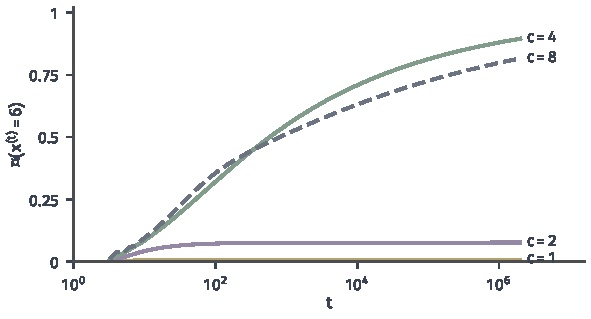
\includegraphics[width=100mm]{figures/05-optimization/05-stochastic-optimization/matplotlib/rs-sa-log-cooling/figure.pdf}
 \caption{对数降温~\eqref{eq:rs-log-cooling}下从$x=2$出发时第$t$步处于全局最小的概率，由双谷链的转移矩阵逐步相乘精确算出。$d^\star=4$，黄、紫两线的$c$小于$d^\star$，绿线取$c=4$，灰色虚线取$c=8$。横轴为对数刻度。}
 \label{fig:rs-sa-log-cooling}
\end{BookInlineFigure}

\paragraph{定理能保证什么}
这个定理的每个条件都要读准。常数$c$要覆盖能垒$d^\star$，而$d^\star$事先通常不知道。定理只对有限状态、对称连通提议成立，提议不对称或被修复过时，要重新核对。

结论是概率的极限，不是“多少步之内一定找到”。七个状态的问题，穷举只要$7$次评价，满足条件的对数降温用了两百万步仍有约一成的概率不在最优解上。$c$取得更大也不是更好：$c=8$在这个时间范围内反而不如$c=4$。

定理也不能换成任意的降温规则。按固定比例降温，$T^{(t)}=T^{(0)}\rho^t$，$0<\rho<1$，这时$\sum_t\exp(-d^\star/T^{(t)})<\infty$，定理的发散条件不满足。下一小节会看到，实际常用的正是这种规则；它能用，但不能借用上面的极限结论。

\subsection{有限预算的退火}
\label{sec:rs-sa-budget}

实际运行时，预算$B$是给定的。这一小节讨论：在$B$次评价之内，温度应当怎样安排，完整流程要包含什么？

\paragraph{三种安排}
第一种是\textbf{固定温度}，全程$T$不变，一共$B$步。第二种是\term{几何降温}（geometric cooling），每隔若干步把温度乘以比例$\rho\in(0,1)$：
\begin{equation}
 T^{[\ell]}=T^{[0]}\rho^{\ell},\qquad\ell=0,1,\ldots,K-1.
 \label{eq:rs-geometric}
\end{equation}
这里$\ell$是温度的层号，用方括号上标与迭代步区分。第三种是\textbf{分段降温}，事先列出几个温度，每个温度跑一段。

一层温度上尝试$M$次提议，共$K$层，那么一次提议就是一次评价，加上起点的一次，总评价次数是
\begin{equation}
 B=1+KM.
 \label{eq:rs-sa-budget}
\end{equation}
预算一定时，层数多则每层短，$\rho$接近$1$时降得慢。预算增加时应当把降温拉长，而不是在同样的降温后面接一段低温下的原地踏步。

\paragraph{温度的尺度}
上一小节说过，温度要和代价尺度配套。常用办法是用初始的上坡量定温度。若典型的上坡量是$\bar{\Delta}$，希望初始接受概率是$\chi_0$，那么由$\exp(-\bar{\Delta}/T^{[0]})=\chi_0$，得到
\begin{equation}
 T^{[0]}=\frac{\bar{\Delta}}{\ln(1/\chi_0)}.
 \label{eq:rs-initial-temp}
\end{equation}

双谷问题的上坡量多为$2$，取$\chi_0=0.6$，得
\[
 T^{[0]}=\frac{2}{\ln(1/0.6)}\approx3.9,
\]
可取$T^{[0]}=4$。结束温度取到上坡几乎不被接受，比如$0.1$，这时上坡量$2$的接受概率约为$2\times10^{-9}$。$\bar{\Delta}$可以先随机试若干对邻居来估计，这些试探也要记入评价次数。

提议的尺度是另一个独立的量。温度决定“接不接受”，邻域大小决定“提议走多远”。把温度调高，并不会让提议跳得更远。

\paragraph{预算内的结果}
图~\ref{fig:rs-sa-schedules}在双谷链上比较四种安排，每种安排都按预算$B$重新拉伸，并用吸收链精确计算“前$B$步内到过$x=6$”的概率。几何降温从$4$到$0.1$；分段降温依次用$4,2,1,0.5,0.25$；固定温度取$T=1$；对数降温取$c=4$。

预算为$10^4$时，几何、分段和固定温度三种安排都几乎必然到过全局最小，只有对数降温的概率约为$0.80$。对数降温在小预算时略占优势，到了大预算反而落后：它在高温停留很短，后面长时间逗留在约$0.5$的低温，翻过能垒的机会稀少。

\begin{BookInlineFigure}
 \centering
 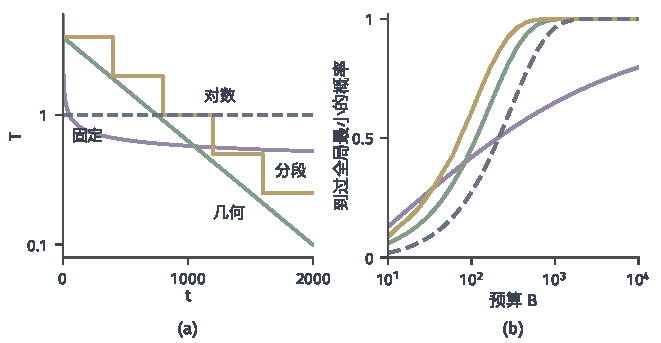
\includegraphics[width=112mm]{figures/05-optimization/05-stochastic-optimization/matplotlib/rs-sa-schedules/figure.pdf}
 \caption{双谷链上的降温安排比较。紫线为对数降温$c=4$，绿线为几何降温（$4\to0.1$），黄线为分段降温，灰色虚线为固定温度$T=1$。(a)预算$B=2000$时的温度，纵轴对数刻度。(b)预算$B$之内到过全局最小的精确概率。}
 \label{fig:rs-sa-schedules}
\end{BookInlineFigure}

这里要分清两个量。“到过”对应最好记录；“结束时停在那里”对应当前状态。预算$10^4$时，结束时处于$x=6$的概率，几何降温约为$0.79$，分段降温约为$0.75$，对数降温约为$0.71$，固定温度$T=1$约为$0.57$。固定温度下最好记录几乎一定拿到最优，当前状态却只有$\pi_1(6)\approx0.57$。

这也回答了为什么最好记录必须写进流程：不写它，固定温度下交出的当前状态有四成多的概率不是最优解。

\paragraph{完整流程}
把前面的决定合起来，一次带重启的退火这样组织。先确定预算$B$，试探代价尺度，由式~\eqref{eq:rs-initial-temp}定$T^{[0]}$，选结束温度、比例$\rho$和每层步数$M$，使总评价满足预算。

然后运行提议、接受和记录更新，每完成一层就降温。一次退火结束后，若预算还有剩余，就从新的起点重新开始，保留全局的最好记录。若单次运行成功的概率是$p$，独立重启$K$次，至少成功一次的概率是
\begin{equation}
 1-(1-p)^K.
 \label{eq:rs-restart}
\end{equation}
例如$p=0.2$，$K=5$，得到$1-0.8^5\approx0.67$。把预算切成几次短运行，单次的$p$会变小，所以切多少份要依问题试验确定。

图~\ref{fig:rs-sa-path}是二维Rastrigin函数上一次预算为$3000$的运行。高温阶段当前点在各个小坑之间跳动，代价可以高到几十；温度降低后渐渐落入一个小坑，后期几乎不再接受上坡。这次运行的最好记录为$(-0.004,0.034)$，代价约为$0.23$。

这是这一次运行得到的结果，换一个种子结果就可能不同。在有限预算下，这样的方法要按运行结果的分布评价，不能因为存在对数降温的极限定理，就说它“能收敛到全局最优”。第~\ref{sec:rs-evaluation}节回到如何评价的问题。

\begin{BookInlineFigure}
 \centering
 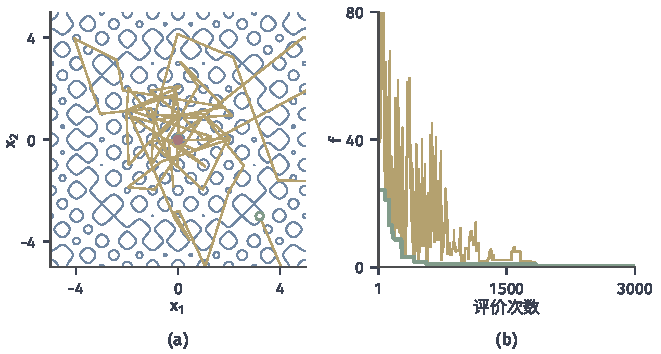
\includegraphics[width=112mm]{figures/05-optimization/05-stochastic-optimization/matplotlib/rs-sa-path/figure.pdf}
 \caption{二维Rastrigin函数~\eqref{eq:rs-rastrigin}上的一次模拟退火，高斯提议$\sigma=0.8$，温度从$25$几何下降到$0.05$，$B=3000$，种子固定。(a)蓝线是等高线，黄线是当前状态的路径（每隔$18$步取一点），空心圆是起点，绿点是最好记录，红点是全局最小点。(b)黄线是当前状态的代价，绿线是最好记录的代价。}
 \label{fig:rs-sa-path}
\end{BookInlineFigure}

\section{演化策略}
\label{sec:rs-es}

模拟退火只有一个状态，提议的形状事先给定。连续变量上还有一种选择：不维护候选，而维护一个“下一批候选从哪里抽”的分布，并让评价结果来修改这个分布。怎样根据一批候选的好坏，调整分布的中心、尺度和形状？这类方法称为\term{演化策略}（evolution strategy，ES）。

一代的流程是：抽出若干候选（称为\term{后代}，offspring），评价，选出较好的（称为\term{亲代}，parents），再由亲代决定下一代的分布。这里的“亲代”“后代”只是名称，所有内容都由下面的公式定义。本节用$\mu$表示亲代个数，$\lambda$表示后代个数，两者都是正整数，不再表示强凸常数和乘子。

\subsection{变异与重组}
\label{sec:rs-es-mutation}

后代从亲代而来。这一小节的问题是：单个后代怎样产生，有多个亲代时又怎样利用它们？

\paragraph{高斯变异}
从亲代$\bm{x}$产生后代的基本方式是加一个高斯扰动：
\begin{equation}
 \bm{y}=\bm{x}+\sigma\bm{z},\qquad\bm{z}\sim\mathcal{N}(\bm{0},\bm{I}),
 \label{eq:rs-mutation}
\end{equation}
称为\term{高斯变异}（Gaussian mutation）。步长$\sigma>0$控制扰动的整体尺度，各向同性指的是所有方向的扰动幅度相同。

用全卷的二次例子$f(\bm{x})=\tfrac12(x_1^2+9x_2^2)$手算一次。在$\bm{x}=(9,1)$处，$f=45$。取$\sigma=1$，抽到$\bm{z}=(-0.8,-0.5)$，后代是$(8.2,0.5)$，代价为
\[
 \tfrac12(67.24+2.25)\approx34.75,
\]
比亲代好，留下。抽到$\bm{z}=(-0.2,0.9)$时，后代是$(8.8,1.9)$，代价约为$54.97$，变差，丢弃。这样只保留变好的结果，就是最简单的$(1+1)$策略，名字的含义下一小节解释。

\paragraph{各向同性的局限}
这个目标在$x_2$方向比$x_1$方向陡$9$倍。图~\ref{fig:rs-es-isotropic}(a)在$(9,1)$周围取$\sigma=2$抽$60$个后代，绿点代价下降，红圈代价上升。圆形的云团和拉长的等高线不匹配：往$x_2$方向稍远一点就越出了等高线。

图~\ref{fig:rs-es-isotropic}(b)用$8\times10^5$个样本估计改善的概率。$\sigma$趋于零时，等高线局部接近直线，改善概率趋于$1/2$；$\sigma$增大，各向同性的抽样在$\sigma\approx2$时约为$0.31$，而沿等高线拉伸的抽样（两个方向的标准差比为$3:1$，面积相同）仍约有$0.42$。

\begin{BookInlineFigure}
 \centering
 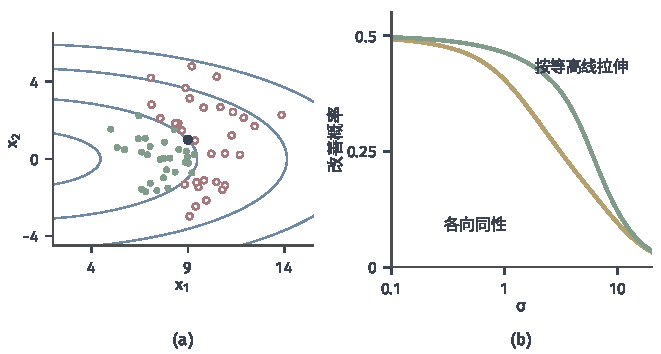
\includegraphics[width=112mm]{figures/05-optimization/05-stochastic-optimization/matplotlib/rs-es-isotropic/figure.pdf}
 \caption{$f=\tfrac12(x_1^2+9x_2^2)$上的变异，亲代在$(9,1)$。(a)蓝线是等高线，深色点是亲代，$\sigma=2$的各向同性后代中绿点改善、红圈变差。(b)改善概率随$\sigma$的变化，黄线为各向同性抽样，绿线的两个坐标标准差分别为$\sqrt3\sigma$和$\sigma/\sqrt3$，由固定种子抽样估计。}
 \label{fig:rs-es-isotropic}
\end{BookInlineFigure}

所以固定的圆形变异有两个问题：$\sigma$要随进展变化，形状也应当贴合地形。后面两小节分别解决。

\paragraph{多个亲代：选一个还是合成一个}
有多个亲代时，有两种产生后代的方式。一种是每次选一个亲代，在它周围变异。另一种是先把亲代合成一个点，称为\term{重组}（recombination），再从这一点变异，比如取权重$w_1\geq\cdots\geq w_\mu>0$，$\sum_iw_i=1$，按代价从好到差排序，
\begin{equation}
 \bm{m}=\sum_{i=1}^{\mu}w_i\bm{x}_{i:\lambda},
 \label{eq:rs-recombination}
\end{equation}
下标$i:\lambda$表示$\lambda$个后代中第$i$好的那个。

取两个亲代手算。$\bm{x}_{1:\lambda}=(7,-0.8)$的代价为$27.38$，$\bm{x}_{2:\lambda}=(8,0.6)$的代价为$33.62$。权重取$(3/4,1/4)$，重组后得到
\[
 \bm{m}=\tfrac34(7,-0.8)+\tfrac14(8,0.6)=(7.25,-0.45),\qquad f(\bm{m})\approx27.19.
\]
重组点比两个亲代都好。

原因在于两个亲代沿$x_2$的偏差一正一负，平均后相互抵消，$x_2$方向的代价又贵，于是抵消的好处很大。这是重组的一种效果：把各个亲代中互不相关的扰动平均掉，保留它们共有的移动。这也不是必然的结果，两个亲代偏差同号时重组就没有这个好处。

\paragraph{两类量}
演化策略中有两类量要分开。一类是\textbf{待优化变量}，就是候选$\bm{x}$本身，提交给$f$评价。另一类是\textbf{策略参数}，如$\sigma$和后面的协方差，它们决定怎样抽样，不提交给$f$，却随代更新。

\subsection{亲代选择}
\label{sec:rs-es-selection}

一代产生了$\lambda$个后代，下一代的亲代应从谁中选？这一小节比较两种规则，并说明它们各自能保证什么。

\paragraph{两种规则}
$(\mu+\lambda)$策略从$\mu$个旧亲代和$\lambda$个后代的并集中选出最好的$\mu$个。$(\mu,\lambda)$策略只从$\lambda$个后代中选最好的$\mu$个，旧亲代全部丢弃，因此要求$\lambda\geq\mu$；$\lambda=\mu$时全部后代都入选，就没有选择了，实际要取$\lambda>\mu$。

前面的$(1+1)$就是一个亲代、一个后代，留下较好者的规则。

\begin{theorem}[保留亲代时最好值不增]
\label{thm:rs-elitist}
设评价无噪声，亲代的代价是准确的。采用$(\mu+\lambda)$选择时，记第$t$代亲代中的最小代价为$f_{\min}^{(t)}$，则
\begin{equation}
 f_{\min}^{(t+1)}\leq f_{\min}^{(t)},\qquad t=0,1,\ldots.
 \label{eq:rs-elitist}
\end{equation}
\end{theorem}

\begin{proof}
第$t$代代价最小的亲代属于第$t+1$代选择的并集。选择取并集中最好的$\mu$个，所以并集的最小代价一定入选，而并集的最小代价不超过$f_{\min}^{(t)}$。
\end{proof}

\paragraph{这个保证的边界}
最好值不增不等于在进步，更不等于走向全局最优。把$(1+1)$规则放在双谷问题上，变异只提议左右相邻的状态，从$x=2$出发，两个邻居都更差，永远不会有后代入选。式~\eqref{eq:rs-elitist}成立，算法却永远停在$f=1$。

高斯变异的支撑是全空间，任何点都有正的概率被抽到，但一次跳过很宽的障碍的概率随距离指数下降，这个正概率在有限预算下没有意义。旧亲代保留也可能拖累搜索：一个特别好的旧亲代长期占据位置，后代都比不过它，$\sigma$的调整也因此失去依据。

\paragraph{两种规则的对比}
图~\ref{fig:rs-es-plus-comma}(a)在二次目标上用固定的$\sigma=0.5$，$\lambda=5$，$\mu=1$。保留亲代时曲线单调下降，到第$80$代代价约为$0.0026$。整代替换时，每一代的亲代都是新的，到了尺度$\sigma$能分辨的精度后就在附近上下波动，第$80$代当前代价约为$0.10$，只有其最好记录（虚线）约为$0.0016$。

图~\ref{fig:rs-es-plus-comma}(b)换到二维Rastrigin函数，$\sigma=0.45$，$40$次独立运行取中位数，起点$(2,2)$，代价为$8$。保留亲代时前期被小坑拦住，改进较慢；整代替换的最好记录（虚线）早期下降更快，因为当前点可以连续穿过小坑，但它的当前代价一直在$10$到$14$之间摆动，到$200$代时中位数约为$14$，而保留亲代的中位数约为$0.39$，整代替换的最好记录约为$0.85$。

\begin{BookInlineFigure}
 \centering
 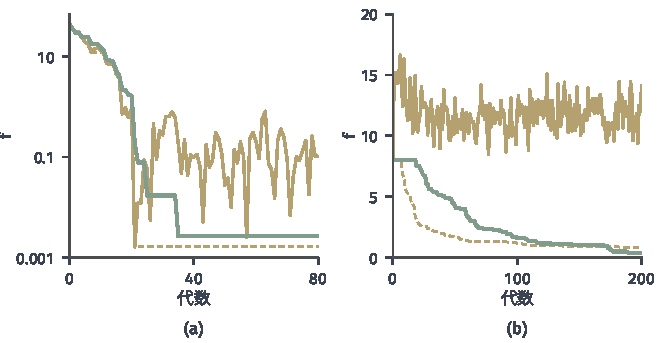
\includegraphics[width=112mm]{figures/05-optimization/05-stochastic-optimization/matplotlib/rs-es-plus-comma/figure.pdf}
 \caption{保留亲代（绿线）与整代替换（黄色实线为当前亲代的代价，黄色虚线为其历史最好）的对比，$\mu=1$，$\lambda=5$，$\sigma$固定。(a)$f=\tfrac12(x_1^2+9x_2^2)$，$\sigma=0.5$，一次运行，纵轴对数刻度。(b)二维Rastrigin函数，$\sigma=0.45$，$40$次运行的中位数，线性纵轴。}
 \label{fig:rs-es-plus-comma}
\end{BookInlineFigure}

\begin{BookInlineTable}
 \centering
 \caption{两种亲代选择的对比。}
 \label{tab:rs-plus-comma}
 \begin{tabular}{lll}
  \toprule
  & $(\mu+\lambda)$ & $(\mu,\lambda)$ \\
  \midrule
  旧亲代 & 与后代竞争 & 全部丢弃 \\
  无噪声时亲代最好值 & 不增 & 可能上升 \\
  是否需要单独保存最好记录 & 不必（已含在亲代中） & 必须 \\
  好亲代长期占位 & 可能 & 不会 \\
  \bottomrule
 \end{tabular}
\end{BookInlineTable}

两种规则都需要配合下面的尺度和形状更新。选择只决定谁留下，走多远、朝哪个形状抽，还要靠策略参数。

\subsection{协方差适应}
\label{sec:rs-es-cma}

圆形的抽样不贴合地形，这一小节的问题是：怎样让抽样分布的形状从评价结果中学出来？

\paragraph{主要思想}
把圆形的扰动换成椭圆形，后代从下式抽取：
\begin{equation}
 \bm{x}_i^{(t+1)}=\bm{m}^{(t)}+\sigma^{(t)}\bm{y}_i,\qquad\bm{y}_i\sim\mathcal{N}(\bm{0},\bm{\Sigma}^{(t)}),\quad i=1,\ldots,\lambda.
 \label{eq:rs-cma-sample}
\end{equation}
这里$\bm{m}^{(t)}$是分布的中心，$\sigma^{(t)}$是整体尺度，对称正定矩阵$\bm{\Sigma}^{(t)}$描述形状。\term{协方差矩阵适应演化策略}（covariance matrix adaptation evolution strategy，CMA-ES）的思路是：让“抽到好后代的那些位移”的分布，成为下一代的抽样分布。

好后代位移的方向多次出现，就说明沿那个方向走有好处，下次沿这个方向多抽一些。可以这样对应：等高线是一条拉长的山谷，中心$\bm{m}$是当前站立的位置，$\bm{\Sigma}$是下一次向四周探路时的步幅分配，把更多的步幅给谷底的走向。

具体的目标用旋转过的椭圆：
\begin{equation}
 f(\bm{x})=\frac12\bm{x}^\top\bm{A}\bm{x},\qquad
 \bm{A}=\begin{bmatrix}5&-4\\-4&5\end{bmatrix}.
 \label{eq:rs-rotated}
\end{equation}
$\bm{A}$的特征值是$1$和$9$，对应的特征方向是$(1,1)$和$(1,-1)$，所以山谷沿$(1,1)$方向。这种倾斜不能靠给两个坐标各设一个步长来表示，必须有非对角元。

更新分三步。第一步按评价排序，只用排序不用代价的数值，取前$\mu$个$\bm{y}_{i:\lambda}$。中心向它们的加权平均移动，权重$w_i$为正，和为$1$：
\begin{equation}
 \bm{y}_w=\sum_{i=1}^{\mu}w_i\bm{y}_{i:\lambda},\qquad
 \bm{m}^{(t+1)}=\bm{m}^{(t)}+\sigma^{(t)}\bm{y}_w.
 \label{eq:rs-cma-mean}
\end{equation}

第二步累积一条路径。一代的$\bm{y}_w$里有随机成分，但真实的好方向会在连续几代中重复出现。把连续几代的$\bm{y}_w$累加起来，得到\term{演化路径}（evolution path）：
\begin{equation}
 \bm{p}_c^{(t+1)}=(1-c_c)\bm{p}_c^{(t)}+\sqrt{c_c(2-c_c)\mu_w}\,\bm{y}_w,\qquad
 \mu_w=\frac{1}{\sum_iw_i^2},
 \label{eq:rs-cma-pc}
\end{equation}
其中$c_c\in(0,1]$决定记忆长度。$\mu_w$是有效亲代数，权重越平均越大。系数$\sqrt{c_c(2-c_c)\mu_w}$的来历在下一小节解释。

第三步更新协方差，把三部分加起来：
\begin{equation}
 \bm{\Sigma}^{(t+1)}=(1-c_1-c_\mu)\bm{\Sigma}^{(t)}
 +c_1\bm{p}_c^{(t+1)}\bigl(\bm{p}_c^{(t+1)}\bigr)^\top
 +c_\mu\sum_{i=1}^{\mu}w_i\bm{y}_{i:\lambda}\bm{y}_{i:\lambda}^\top.
 \label{eq:rs-cma-cov}
\end{equation}
第一部分是旧的形状，第二部分来自路径方向，称为秩一更新，第三部分是这一代选中位移的加权协方差，称为秩$\mu$更新。

式~\eqref{eq:rs-cma-cov}的$\bm{y}_{i:\lambda}$是相对旧中心的位移，用的是旧的$\bm{m}$。如果用新的$\bm{m}$，等于把这一代沿平均方向的进展减掉了，协方差就只记录了后代之间的散布，看不出朝哪边走有好处。

\paragraph{协方差保持正定}
抽样要求$\bm{\Sigma}$正定，下面的引理说明正权重时自动满足。

\begin{lemma}[协方差更新保持正定]
\label{lem:rs-cma-pd}
设$\bm{\Sigma}^{(t)}$对称正定，$c_1,c_\mu\geq0$，$c_1+c_\mu<1$，$w_i>0$。则由式~\eqref{eq:rs-cma-cov}得到的$\bm{\Sigma}^{(t+1)}$对称正定。
\end{lemma}

\begin{proof}
任取$\bm{u}\neq\bm{0}$，由式~\eqref{eq:rs-cma-cov}，
\[
 \bm{u}^\top\bm{\Sigma}^{(t+1)}\bm{u}
 =(1-c_1-c_\mu)\bm{u}^\top\bm{\Sigma}^{(t)}\bm{u}
 +c_1\langle\bm{u},\bm{p}_c^{(t+1)}\rangle^2
 +c_\mu\sum_iw_i\langle\bm{u},\bm{y}_{i:\lambda}\rangle^2.
\]
第一项为正，后两项非负。对称性由三个对称矩阵之和得到。
\end{proof}

这里假定权重全为正。有的实现给排序靠后的后代分配负权重，用来主动缩小不好的方向，那时要专门限制幅度，上面的引理不再适用。

\needspace{6\baselineskip}
\paragraph{变量}
下面用目标~\eqref{eq:rs-rotated}手算一代。要维护的量是：
\begin{itemize}
 \item $\bm{m}^{(t)}\in\mathbb{R}^n$：中心，$\sigma^{(t)}>0$：整体尺度；
 \item $\bm{\Sigma}^{(t)}\in\mathbb{R}^{n\times n}$：形状，对称正定；
 \item $\bm{p}_c^{(t)}\in\mathbb{R}^n$：协方差路径，$\bm{p}_\sigma^{(t)}\in\mathbb{R}^n$：步长路径，下一小节使用；
 \item 最好记录。整代替换时中心本身未必被评价过，记录必须单独保存。
\end{itemize}

\paragraph{初始化}
中心取$\bm{m}^{(0)}$，尺度取一个足以覆盖初始不确定性的量，形状取单位阵，两条路径取零。例中为了手算，把参数取成简单的数：
\[
 \bm{m}^{(0)}=\begin{bmatrix}3\\1\end{bmatrix},\qquad\sigma^{(0)}=1,\qquad\bm{\Sigma}^{(0)}=\bm{I},\qquad\bm{p}_c^{(0)}=\bm{p}_\sigma^{(0)}=\bm{0},
\]
\[
 \lambda=4,\quad\mu=2,\quad(w_1,w_2)=\bigl(\tfrac34,\tfrac14\bigr),\quad c_c=\tfrac12,\quad c_1=c_\mu=\tfrac15.
\]
于是$\mu_w=1/(9/16+1/16)=1.6$，路径系数$\sqrt{c_c(2-c_c)\mu_w}=\sqrt{1.2}\approx1.095$。此时$f(\bm{m}^{(0)})=13$。实际运行时参数按维数取默认公式，这里的简单数值只为演示。

\paragraph{每轮更新}
第$t$代依次执行以下步骤，直到预算用完或$\sigma$小到分辨不出差别。

\begin{enumerate}
 \item 由式~\eqref{eq:rs-cma-sample}抽$\lambda$个后代并评价，这一步要做$\lambda$次评价。例中$\bm{\Sigma}^{(0)}=\bm{I}$，取四个位移，后代和代价是
 \[
  \begin{gathered}
  \bm{y}_1=(-1,-0.6):\ \bm{x}_1=(2,0.4),\ f=7.2,\\
  \bm{y}_2=(0.5,0.5):\ \bm{x}_2=(3.5,1.5),\ f=15.25,\\
  \bm{y}_3=(-0.4,-1):\ \bm{x}_3=(2.6,0),\ f=16.9,\\
  \bm{y}_4=(1,-0.5):\ \bm{x}_4=(4,0.5),\ f=32.625.
  \end{gathered}
 \]
 \item 按代价排序，更新最好记录。例中顺序就是$1,2,3,4$，记录为$(2,0.4)$，代价$7.2$。
 \item 由式~\eqref{eq:rs-cma-mean}更新中心。例中
 \[
  \bm{y}_w=\tfrac34\begin{bmatrix}-1\\-0.6\end{bmatrix}+\tfrac14\begin{bmatrix}0.5\\0.5\end{bmatrix}=\begin{bmatrix}-0.625\\-0.325\end{bmatrix},\qquad
  \bm{m}^{(1)}=\begin{bmatrix}2.375\\0.675\end{bmatrix}.
 \]
 新中心的代价约为$8.83$，它没有被评价，这里只是核对。
 \item 更新步长路径$\bm{p}_\sigma$，见下一小节。
 \item 由式~\eqref{eq:rs-cma-pc}更新协方差路径。例中$\bm{p}_c^{(0)}=\bm{0}$，
 \[
  \bm{p}_c^{(1)}=1.095\,\bm{y}_w\approx\begin{bmatrix}-0.685\\-0.356\end{bmatrix}.
 \]
 \item 由式~\eqref{eq:rs-cma-cov}更新协方差。例中秩$\mu$部分是
 \[
  \tfrac34\begin{bmatrix}1&0.6\\0.6&0.36\end{bmatrix}+\tfrac14\begin{bmatrix}0.25&0.25\\0.25&0.25\end{bmatrix}=\begin{bmatrix}0.8125&0.5125\\0.5125&0.3325\end{bmatrix},
 \]
 秩一部分是
 \[
  \bm{p}_c^{(1)}\bigl(\bm{p}_c^{(1)}\bigr)^\top\approx\begin{bmatrix}0.469&0.244\\0.244&0.127\end{bmatrix},
 \]
 于是
 \[
  \bm{\Sigma}^{(1)}=0.6\,\bm{I}+0.2\,(\text{秩一})+0.2\,(\text{秩}\mu)\approx\begin{bmatrix}0.856&0.151\\0.151&0.692\end{bmatrix}.
 \]
 \item 更新$\sigma$，见下一小节。
\end{enumerate}

第一代结束，非对角元从$0$变成了正的$0.151$，大特征值$0.946$对应的方向约为$(0.86,0.51)$，已经朝山谷方向$(1,1)$倾斜了一点。最终在这一代得到中心$(2.375,0.675)$与记录$(2,0.4)$，后续各代重复以上步骤。

\paragraph{形状在做什么，以及它不是什么}
图~\ref{fig:rs-cma-adapt}取$n=2$的默认参数（$\lambda=6$，$\mu=3$）从$(5,-1)$出发。左图中椭圆起初是圆，几代之后沿山谷拉长，然后整体缩小。右图把$\bm{\Sigma}$的行列式归一后叠在一起：第$40$代的椭圆长短轴之比的平方约为$7.2$，方向与山谷一致，形状接近$\bm{A}^{-1}$的椭圆（比值为$9$）。

\begin{BookInlineFigure}
 \centering
 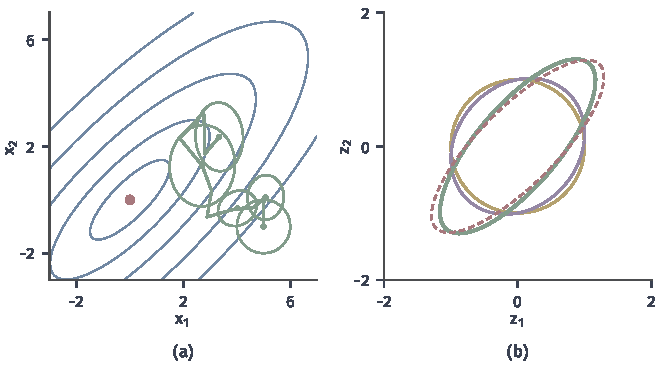
\includegraphics[width=112mm]{figures/05-optimization/05-stochastic-optimization/matplotlib/rs-cma-adapt/figure.pdf}
 \caption{CMA-ES在式~\eqref{eq:rs-rotated}上的一次运行，默认参数，$\lambda=6$，种子固定。(a)蓝线是等高线，绿线是中心的路径，绿色椭圆是第$0,2,4,7,11$代的$\sigma\bm{\Sigma}^{1/2}$单位圆像。(b)把$\bm{\Sigma}$的行列式归一化后的形状：黄线第$0$代，紫线第$6$代，绿线第$40$代，红色虚线是同样归一化的$\bm{A}^{-1}$。}
 \label{fig:rs-cma-adapt}
\end{BookInlineFigure}

在二次目标上，$\bm{\Sigma}$大致正比于$\bm{A}^{-1}$是可以理解的：作坐标变换$\bm{u}=\bm{A}^{1/2}\bm{x}$后等高线变成圆，而$\bm{\Sigma}\propto\bm{A}^{-1}$的抽样在$\bm{u}$坐标下正好是各向同性的。但这是对运行结果的描述，并不是一个无条件的等式。

一个简单的论证说明两者不可能恒等。CMA-ES只用排序，所以把$f$换成任何严格递增的函数，比如$h=\sqrt{f}$，排序完全不变，同一组随机数给出完全相同的$\bm{\Sigma}$序列。可是在$f>0$的点，
\[
 \nabla^2h=\frac{1}{2\sqrt{f}}\nabla^2f-\frac{1}{4f^{3/2}}\nabla f\nabla f^\top,
\]
它与$\nabla^2f$的形状不同。同一个$\bm{\Sigma}$不能同时是两者的逆。所以搜索协方差不是目标的Hessian，也不无条件地等于它的逆；它记录的是最近一段时间里选中位移的分布，并且依赖种群大小和有限的代数。

只用排序的好处恰恰在这里：算法的行为不随$f$的单调变换改变。这是它与第~\ref{chap:zeroth-order-optimization}章直接用函数值大小构造方向的做法的一个区别。

\subsection{步长适应}
\label{sec:rs-es-step}

协方差$\bm{\Sigma}$描述形状，而$\sigma$描述整体尺度。把两者分开的理由是：尺度需要比形状快得多的调整。这一小节的问题是：只看选中位移，怎样判断$\sigma$太大还是太小？

\paragraph{路径长度}
连续几代的位移如果彼此同向，说明本可以走得更远，$\sigma$偏小。如果彼此反向、互相抵消，说明走过了头在来回摆动，$\sigma$偏大。

图~\ref{fig:rs-cma-path-sigma}(a)(b)画的就是这两种情形：四段长度差不多的位移，同向时首尾相接的总位移很长，来回抵消时总位移很短。所以要比较的是累计路径的长度与“位移彼此无关时的路径长度”。

\begin{BookInlineFigure}
 \centering
 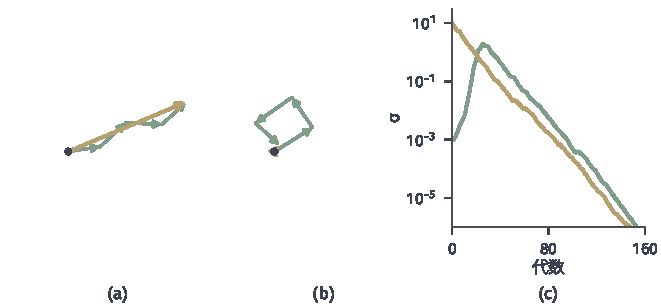
\includegraphics[width=112mm]{figures/05-optimization/05-stochastic-optimization/matplotlib/rs-cma-path-sigma/figure.pdf}
 \caption{路径长度与步长适应。(a)四段位移（绿）大致同向，累计位移（黄）长度约$4.8$。(b)四段位移互相抵消，累计位移长度约$0.2$。(c)五维球面$f=\tfrac12\lVert\bm{x}\rVert_2^2$上$\sigma$随代数的变化，只使用下面的步长路径，从$\sigma^{(0)}=10^{-3}$（绿）和$\sigma^{(0)}=10$（黄）出发，纵轴对数刻度。}
 \label{fig:rs-cma-path-sigma}
\end{BookInlineFigure}

\paragraph{标准化后累积}
为了把形状的影响除掉，累积之前先用$(\bm{\Sigma}^{(t)})^{-1/2}$把位移变成各向同性：
\begin{equation}
 \bm{p}_\sigma^{(t+1)}=(1-c_\sigma)\bm{p}_\sigma^{(t)}+\sqrt{c_\sigma(2-c_\sigma)\mu_w}\,\bigl(\bm{\Sigma}^{(t)}\bigr)^{-1/2}\bm{y}_w.
 \label{eq:rs-cma-psigma}
\end{equation}
再把路径长度与标准正态向量的期望长度比较，据此调整尺度：
\begin{equation}
 \sigma^{(t+1)}=\sigma^{(t)}\exp\Bigl(\frac{c_\sigma}{d_\sigma}\Bigl(\frac{\lVert\bm{p}_\sigma^{(t+1)}\rVert_2}{\mathbb{E}\lVert\bm{z}\rVert_2}-1\Bigr)\Bigr),\qquad\bm{z}\sim\mathcal{N}(\bm{0},\bm{I}).
 \label{eq:rs-cma-sigma}
\end{equation}
其中$d_\sigma>0$是阻尼。路径偏长时$\sigma$增大，偏短时$\sigma$减小。

系数的选取有一个清楚的理由。设选择完全随机，即排序与位移无关。这时$\bm{y}_w\sim\mathcal{N}(\bm{0},\bm{\Sigma}^{(t)}/\mu_w)$，于是$\sqrt{\mu_w}(\bm{\Sigma}^{(t)})^{-1/2}\bm{y}_w$是标准正态向量，记为$\bm{\xi}$。

若$\bm{p}_\sigma^{(t)}$也是标准正态向量，且与$\bm{\xi}$独立，那么式~\eqref{eq:rs-cma-psigma}的两项之和仍是高斯向量，协方差的系数为
\[
 (1-c_\sigma)^2+c_\sigma(2-c_\sigma)=1.
\]
所以随机选择下路径的分布不变，$\lVert\bm{p}_\sigma\rVert_2$的期望等于比较基准，$\sigma$在对数尺度上没有系统漂移。式~\eqref{eq:rs-cma-pc}的系数是同一个道理。一旦有真实选择，路径的长度偏离基准才来自评价信息。

\paragraph{例中的这一步}
接上一小节的第一代，取$c_\sigma=1/2$，$d_\sigma=1$，$\bm{\Sigma}^{(0)}=\bm{I}$，所以由式~\eqref{eq:rs-cma-psigma}，
\[
 \bm{p}_\sigma^{(1)}=1.095\,\bm{y}_w\approx\begin{bmatrix}-0.685\\-0.356\end{bmatrix},\qquad\lVert\bm{p}_\sigma^{(1)}\rVert_2\approx0.772.
\]

二维时$\bm{z}$的期望长度是$\sqrt{\pi/2}\approx1.253$。由式~\eqref{eq:rs-cma-sigma}，
\[
 \sigma^{(1)}=\exp\Bigl(\tfrac12\bigl(\tfrac{0.772}{1.253}-1\bigr)\Bigr)\approx\exp(-0.192)\approx0.825.
\]
路径比基准短，尺度缩小。第一代的路径从零开始，只积累了一代，这个判断偏保守。

图~\ref{fig:rs-cma-path-sigma}(c)是这个规则的效果。$\sigma$起初只有$10^{-3}$时，路径持续同向，$\sigma$在约$25$代内升到接近$2$；起初为$10$时，$\sigma$直接下降。之后两条线都随着接近最优点按稳定的比例减小，代价在$160$代后约为$10^{-13}$量级。

\paragraph{两条路径的职责}
两条路径形式相近，用途不同，表~\ref{tab:rs-two-paths}是对比。

\begin{BookInlineTable}
 \centering
 \caption{两条演化路径。}
 \label{tab:rs-two-paths}
 \begin{tabular}{lll}
  \toprule
  & 协方差路径$\bm{p}_c$ & 步长路径$\bm{p}_\sigma$ \\
  \midrule
  累积的量 & $\bm{y}_w$，含形状 & $\bm{\Sigma}^{-1/2}\bm{y}_w$，已标准化 \\
  用到它的什么 & 方向和符号相关 & 长度 \\
  更新谁 & $\bm{\Sigma}$（秩一项） & $\sigma$ \\
  \bottomrule
 \end{tabular}
\end{BookInlineTable}

\paragraph{更新顺序与数值处理}
一代内的次序是：抽样和评价；更新$\bm{m}$；用旧的$\bm{\Sigma}$更新$\bm{p}_\sigma$；更新$\bm{p}_c$；更新$\bm{\Sigma}$；最后更新$\sigma$。把$\bm{\Sigma}$的更新放在$\sigma$之前，是因为式~\eqref{eq:rs-cma-cov}中的$\bm{y}_{i:\lambda}$已按抽样时的$\sigma^{(t)}$标准化，这时不需要新的尺度。

实际实现还有一个小的修正：当$\lVert\bm{p}_\sigma\rVert_2$异常大，说明$\sigma$正在快速调整，这时暂停式~\eqref{eq:rs-cma-pc}右端的累积，防止形状被一次快速移动带偏。

代价方面，抽样要用$\bm{\Sigma}^{1/2}$，$\bm{p}_\sigma$要用$\bm{\Sigma}^{-1/2}$，这需要对称特征分解，稠密时一次约$O(n^3)$。通常每隔若干代才重新分解一次，把平均开销压到每次评价$O(n^2)$。

数值上要防止协方差病态：每次分解前把$\bm{\Sigma}$强制对称化，检查最小特征值是否仍为正，条件数太大时重置或停止。式~\eqref{eq:rs-cma-sigma}的指数形式保证$\sigma$恒正，无需额外处理。

\subsection{自然演化策略（补充）}
\label{sec:rs-es-nes}

前面的更新公式是逐条设计的。这一小节换一个角度：能不能把搜索分布的参数本身当作优化变量，直接写出它的梯度下降？这样得到的方法称为\term{自然演化策略}（natural evolution strategy，NES）。

\paragraph{分布参数上的目标}
设搜索分布$q_{\bm{\theta}}$由参数$\bm{\theta}$决定，把期望代价作为$\bm{\theta}$的函数：
\begin{equation}
 J(\bm{\theta})=\mathbb{E}_{\bm{x}\sim q_{\bm{\theta}}}[f(\bm{x})]=\int f(\bm{x})q_{\bm{\theta}}(\bm{x})\,\mathrm{d}\bm{x}.
 \label{eq:rs-nes-objective}
\end{equation}

$\bm{x}$可以是离散的，$f$可以不可微，只要$q_{\bm{\theta}}$对$\bm{\theta}$光滑。在可交换微分与积分的条件下，
\[
 \nabla_{\bm{\theta}}J(\bm{\theta})=\int f(\bm{x})\nabla_{\bm{\theta}}q_{\bm{\theta}}(\bm{x})\,\mathrm{d}\bm{x}.
\]

再把$\nabla q$写成$q\nabla\log q$，得到可以用样本估计的形式：
\begin{equation}
 \nabla_{\bm{\theta}}J(\bm{\theta})=\mathbb{E}_{\bm{x}\sim q_{\bm{\theta}}}\bigl[f(\bm{x})\nabla_{\bm{\theta}}\log q_{\bm{\theta}}(\bm{x})\bigr].
 \label{eq:rs-score-gradient}
\end{equation}
其中$\nabla_{\bm{\theta}}\log q_{\bm{\theta}}$称为\term{得分函数}（score function）。

\paragraph{与平滑估计的交叉}
取$q=\mathcal{N}(\bm{m},\sigma^2\bm{I})$，只把中心$\bm{m}$当参数，$\sigma$固定。写$\bm{x}=\bm{m}+\sigma\bm{z}$，得分是
\[
 \nabla_{\bm{m}}\log q=\frac{\bm{x}-\bm{m}}{\sigma^2}=\frac{\bm{z}}{\sigma}.
\]

代入式~\eqref{eq:rs-score-gradient}，有
\begin{equation}
 \nabla_{\bm{m}}J=\frac{1}{\sigma}\mathbb{E}_{\bm{z}}\bigl[f(\bm{m}+\sigma\bm{z})\bm{z}\bigr].
 \label{eq:rs-nes-gaussian}
\end{equation}
这里的$J$把$f$在$\bm{m}$周围按高斯权重做了平均，这正是第~\ref{chap:zeroth-order-optimization}章的高斯平滑目标，式~\eqref{eq:rs-nes-gaussian}正是那里的高斯方向估计。在这一实例上，分布梯度和平滑梯度是同一件事，这就是本节开头说的两种视角的重合。

一个可手算的例子：$f(x)=x^2$，$q=\mathcal{N}(m,\sigma^2)$，$m=2$，$\sigma=1$。这时精确值是$J=m^2+\sigma^2$，$\partial_mJ=2m=4$。取两个样本$z=\pm1$，读数为$f(3)=9$，$f(1)=1$，估计值为
\[
 \frac12\bigl(9\cdot1+1\cdot(-1)\bigr)=4,
\]
恰好是精确值。一般样本下估计值有方差，只有期望等于$2m$。

\paragraph{基线}
由于$\mathbb{E}[\nabla\log q]=\bm{0}$，给$f$减去一个常数$b$不改变期望，却改变方差。上例中估计量$(f(m+z)-b)z$的方差可以逐项算出。

记$a=m^2-b$，把$(m+z)^2-b$展开，估计量等于$az+2mz^2+z^3$，用$\mathbb{E}z^2=1$，$\mathbb{E}z^4=3$，$\mathbb{E}z^6=15$，奇数阶矩为零，得到
\[
 \operatorname{Var}=a^2+6a+15+8m^2.
\]

$m=2$时，$b=0$（$a=4$）的方差是$87$；$b=5$（$a=-1$）的方差是$42$；$b=7$（$a=-3$）的方差最小，是$38$。基线不改变估计的目标，只改变噪声大小。

\paragraph{自然梯度}
普通梯度依赖参数怎样写。把$\sigma$换成$\log\sigma$，梯度的方向就变了，可分布族是同一个。自然的办法是用分布之间的差别来度量参数的变化，即用\term{Fisher信息矩阵}（Fisher information matrix）
\begin{equation}
 \bm{F}(\bm{\theta})=\mathbb{E}_{\bm{x}\sim q_{\bm{\theta}}}\bigl[\nabla_{\bm{\theta}}\log q_{\bm{\theta}}(\bm{x})\nabla_{\bm{\theta}}\log q_{\bm{\theta}}(\bm{x})^\top\bigr]
 \label{eq:rs-fisher}
\end{equation}
作度量，沿\term{自然梯度}（natural gradient）下降：
\begin{equation}
 \bm{\theta}^{(t+1)}=\bm{\theta}^{(t)}-\eta\,\bm{F}(\bm{\theta}^{(t)})^{-1}\nabla_{\bm{\theta}}J(\bm{\theta}^{(t)}).
 \label{eq:rs-natural-gradient}
\end{equation}

一维高斯$\bm{\theta}=(m,\sigma)$，得分是$(z/\sigma,(z^2-1)/\sigma)$，由$\mathbb{E}z^2=1$，$\mathbb{E}(z^2-1)^2=2$，交叉项为$\mathbb{E}z(z^2-1)=0$，得
\[
 \bm{F}=\begin{bmatrix}1/\sigma^2&0\\0&2/\sigma^2\end{bmatrix}.
\]

还是目标$J=m^2+\sigma^2$，普通梯度是$(2m,2\sigma)$，自然梯度是
\[
 \bm{F}^{-1}\nabla J=(2m\sigma^2,\ \sigma^3).
\]
在$(m,\sigma)=(2,1)$，普通梯度是$(4,2)$，自然梯度是$(4,1)$。

图~\ref{fig:rs-nes-flow}比较两条连续轨迹。普通梯度沿直线同比例缩小$m$和$\sigma$。自然梯度下由$\mathrm{d}m/\mathrm{d}\sigma=2m/\sigma$得$m\propto\sigma^2$，均值比宽度收得快，分布先把中心挪到位，再缩小探索范围。

\begin{BookInlineFigure}
 \centering
 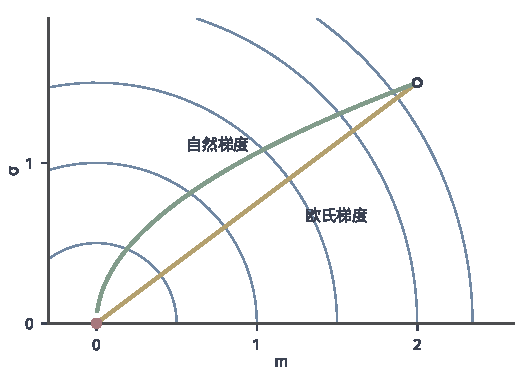
\includegraphics[width=88mm]{figures/05-optimization/05-stochastic-optimization/matplotlib/rs-nes-flow/figure.pdf}
 \caption{分布参数平面上的两条下降路径，$J(m,\sigma)=m^2+\sigma^2$，蓝线是$J$的等值线，空心圆是起点$(2,1.5)$，红点是最小点。黄线沿普通梯度，绿线沿自然梯度，后者满足$m\propto\sigma^2$。}
 \label{fig:rs-nes-flow}
\end{BookInlineFigure}

\paragraph{和CMA-ES的关系，以及要核对什么}
把$\bm{\theta}$限于中心，并把$f$换成按排序给的效用：选中的后代权重$w_i$，其余为$0$。对$\mathcal{N}(\bm{m},\sigma^2\bm{\Sigma})$，Fisher矩阵的均值块是$(\sigma^2\bm{\Sigma})^{-1}$，自然梯度下的均值更新量是
\[
 \sigma^2\bm{\Sigma}\cdot\sum_iw_i(\sigma^2\bm{\Sigma})^{-1}(\bm{x}_{i:\lambda}-\bm{m})=\sigma\sum_iw_i\bm{y}_{i:\lambda},
\]
这正是式~\eqref{eq:rs-cma-mean}。

这里有一点要小心：把$f$换成排序效用后，优化的已经不是原来的$J$，排序依赖当前样本，估计量也不再是式~\eqref{eq:rs-score-gradient}的无偏估计。基线只改变方差，排序效用改变了目标，把尺度参数写成$\sigma$还是$\log\sigma$则改变普通梯度的方向，这三件事不能混为一谈。说一个更新“是梯度下降”时，要先说清是哪个目标、哪个估计量、哪种度量。


\section{遗传算法}
\label{sec:rs-ga}

演化策略的搜索分布依赖连续变量的高斯结构，换到开关选择或排列上就用不上了。于是要问：候选是离散的编码时，怎样利用一批已评价的候选产生新的候选？\term{遗传算法}（genetic algorithm，GA）的做法是：维护一个种群，用评价选出亲代，把亲代的编码拼接和改动，得到新的候选。

“基因”“繁殖”只是沿用下来的名称。这些类比并不告诉我们一个操作在实际问题上做了什么。下面把四件事分开说明：候选的编码、亲代的选择、新候选的产生、下一代的组成。

\subsection{候选解的编码}
\label{sec:rs-ga-encoding}

遗传算法的操作都作用在编码上。这一小节的问题是：候选应当怎样写成编码，编码与原问题的解是什么关系？

\paragraph{选择问题：0--1串}
全节用一个背包问题作例子。有六件物品，第$j$件价值$v_j$、重量$w_j$，容量为$15$：
\[
 \bm{v}=(6,5,8,9,6,7),\qquad\bm{w}=(2,3,6,7,5,9).
\]

用串$\bm{b}\in\{0,1\}^6$表示选择，$b_j=1$表示选第$j$件。要最小化的是价值的相反数：
\begin{equation}
 f(\bm{b})=-\sum_{j=1}^{6}v_jb_j,\qquad\text{约束}\quad\sum_{j=1}^{6}w_jb_j\leq15.
 \label{eq:rs-knapsack}
\end{equation}
例如$\bm{b}=101100$选第$1,3,4$件，总重$15$，$f=-23$。穷举全部$2^6=64$个串可知这正是最优解，总共$30$个可行串。

\term{解码}（decoding）是从编码回到原问题的解，评价永远在解码之后进行。这里编码与解是一一对应的，解码平凡，但重量约束使得并非每个串都可行，第~\ref{sec:rs-constraints}节处理这一点。

\paragraph{顺序问题：排列}
访问顺序、任务排程的自然编码是排列，第~\ref{sec:rs-space}节的$ABDCE$就是一个例子，排列本身就是解。

把排列硬写成二进制会带来麻烦。五个元素每个用三位表示，一共$15$位，有$2^{15}=32768$种串，其中只有$5!=120$种是合法排列，约占$0.37\%$。翻一位多半得到重复元素的串，算法大部分精力花在非法候选上。

\paragraph{连续变量}
连续变量可以直接用实数向量编码，第~\ref{sec:rs-evaluation}节的比较实验就是这样做的，这时“交叉”是两个实数向量的组合，“变异”是加一个小扰动。

编码决定了什么叫“邻近”，决定了哪些操作合法，所以不存在一种通用的串表示。写清楚编码的含义、解码方式和合法操作，是这类算法要做的第一件事。

\subsection{亲代选择}
\label{sec:rs-ga-parents}

有了种群和评价，下一个问题是：谁来产生下一代的候选？选得太偏向好个体，种群很快只剩少数几种；选得太平均，又等于随机游走。用同一组数比较几种规则。设种群有$N=5$个候选，代价从好到差为
\begin{equation}
 (f_{1:5},\ldots,f_{5:5})=(-24,-20,-19,-15,-10).
 \label{eq:rs-selection-costs}
\end{equation}

\paragraph{排序选择}
把候选按代价排序，只按名次分配概率。线性排序取参数$s\in(1,2]$，第$r$名被选中的概率是
\begin{equation}
 p_r=\frac{1}{N}\Bigl(2-s+2(s-1)\frac{N-r}{N-1}\Bigr).
 \label{eq:rs-rank-selection}
\end{equation}
$s=1.5$，$N=5$时，五个名次的概率是
\[
 (0.30,\ 0.25,\ 0.20,\ 0.15,\ 0.10).
\]
由于只用名次，把代价做单调变换不影响选择。

\paragraph{锦标赛选择}
\term{锦标赛选择}（tournament selection）每次有放回地抽$k$个候选，选其中代价最小的。它不需要排序全体，也只用比较结果。第$r$名被选中，当且仅当这$k$次抽样都不比第$r$名更好（共有$N-r+1$个这样的候选可抽），并且至少有一次抽到了第$r$名。所以
\begin{equation}
 p_r=\frac{(N-r+1)^k-(N-r)^k}{N^k}.
 \label{eq:rs-tournament}
\end{equation}
这里默认没有并列。

$N=5$，$k=2$时，五个名次的概率是
\[
 (0.36,\ 0.28,\ 0.20,\ 0.12,\ 0.04).
\]

$k=3$时是
\[
 (0.488,\ 0.296,\ 0.152,\ 0.056,\ 0.008).
\]
$k$越大，好候选被选中的倾向越强。这种倾向称为\term{选择压力}（selection pressure）。以第$1$名在$N$次选择中的期望份数$Np_1$度量，$k=2$时是$1.8$份，$k=3$时是$2.44$份。

\paragraph{比例选择要先转换}
经典的比例选择把选中概率设为正比于\term{适应度}（fitness）$F$。最小化问题的代价不能直接拿来用：代价越低越好，比例却是数越大份额越大，方向就是反的。

把式~\eqref{eq:rs-selection-costs}的代价都加上$20$，问题没有变，五个数成为$(-4,0,1,5,10)$，总和是$12$，第一个比值是负数，根本不是概率。

必须先指定从代价到非负权重的转换。一种做法是以当前最差者为基准：
\begin{equation}
 F_i=f_{\max}-f_i+\delta,\qquad\delta>0.
 \label{eq:rs-fitness}
\end{equation}
取$\delta=1$，得到权重$(15,11,10,6,1)$，总和为$43$，五个概率约为
\[
 (0.349,\ 0.256,\ 0.233,\ 0.140,\ 0.023).
\]

这个转换对代价的平移不变，但概率依赖代价差的相对大小，也依赖$\delta$的取值，把$\delta$取大，选择会趋于均匀。图~\ref{fig:rs-ga-selection}把几种规则画在一起。

\begin{BookInlineFigure}
 \centering
 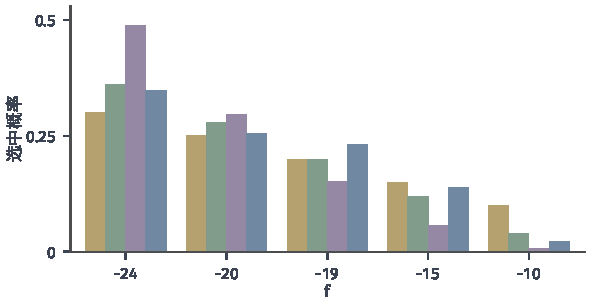
\includegraphics[width=100mm]{figures/05-optimization/05-stochastic-optimization/matplotlib/rs-ga-selection/figure.pdf}
 \caption{同一组代价~\eqref{eq:rs-selection-costs}下五个候选的选中概率，从左到右依次为线性排序（黄，$s=1.5$）、二元锦标赛（绿）、三元锦标赛（紫）、比例选择（蓝，$\delta=1$）。}
 \label{fig:rs-ga-selection}
\end{BookInlineFigure}

\subsection{交叉与变异}
\label{sec:rs-ga-operators}

选出亲代以后，怎样产生新候选？有两种操作，职责不同。\term{交叉}（crossover）把两个亲代已有的片段重新组合，只能产生两个亲代片段的拼接。\term{变异}（mutation）改动个别位置，引入亲代都没有的内容。

\paragraph{二进制串}
\textbf{单点交叉}随机选一个切点，交换切点后的尾部。用两个亲代
\[
 \bm{a}=110\,100,\qquad\bm{b}=101\,010,
\]
切点在第$3$位之后。

$\bm{b}$的前三位接$\bm{a}$的后三位，得到$101\,100$；$\bm{a}$的前三位接$\bm{b}$的后三位，得到$110\,010$。第一个后代正是最优解$101100$，$f=-23$，比两个亲代的$-20$都好。第二个后代$110010$总重$10$，$f=-17$，比两个亲代都差。交叉只是重新组合，不保证任何一个后代更好。

\textbf{逐位变异}对每一位独立以概率$p_m$翻转，常取$p_m=1/n$，平均每个串翻一位。图~\ref{fig:rs-ga-crossover}(a)中第二个后代的第$4$位翻转，变成$110110$。这个串总重$17$，超过容量，是不可行的。

\begin{BookInlineFigure}
 \centering
 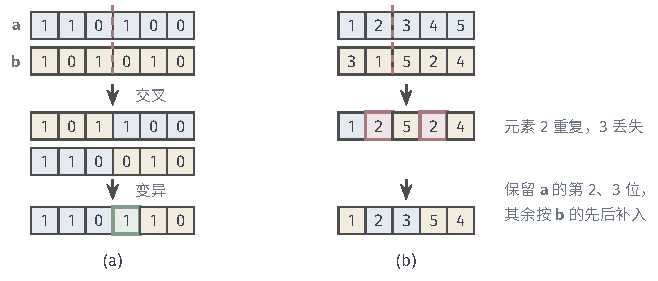
\includegraphics[width=111mm]{figures/05-optimization/05-stochastic-optimization/tikz/rs-ga-crossover/figure.pdf}
 \caption{二进制串与排列上的操作。蓝色格来自亲代$\bm{a}$，黄色格来自亲代$\bm{b}$，红色虚线是切点。(a)单点交叉后，第二个后代的第$4$位变异（绿框）。(b)在排列上直接交换尾部会产生重复元素（红框）；保留$\bm{a}$的中段再按$\bm{b}$的先后顺序补入其余元素，得到合法排列。}
 \label{fig:rs-ga-crossover}
\end{BookInlineFigure}

\paragraph{排列要用保持排列的算子}
排列上的单点交叉会出错。$\bm{a}=12345$，$\bm{b}=31524$，切点在第$2$位之后，直接拼接得到$12\,524$，元素$2$出现两次，元素$3$丢失，已经不是排列。

有两种处理办法：换用保持排列的算子，或者明确规定修复规则。\textbf{顺序交叉}属于前者：保留$\bm{a}$的第$2$、$3$位，即$23$，其余位置按$\bm{b}$中出现的先后依次填入尚未使用的元素，$\bm{b}$的顺序去掉$2,3$后是$1,5,4$，于是得到$12354$。排列上的变异也用交换两个位置或翻转一段，而不用单独改一个位置。

\paragraph{两组参数分开记录}
交叉概率$p_c$是一对亲代发生交叉的概率，不交叉时后代直接复制亲代。变异概率$p_m$是每一位翻转的概率，作用范围是一位而不是一个串。两者要分别记录。

两种操作各自都不保证改善目标。上面的例子里，同一次交叉同时给出了最好的和较差的后代，一次变异把后代变得不可行。质量的提升要靠后面的选择来累积。

\subsection{后代替换}
\label{sec:rs-ga-replacement}

亲代选择决定谁来产生新候选，后代替换决定谁进入下一代，两者是两个独立的决定。

\paragraph{三种替换}
\textbf{整代替换}用后代完全替代上一代。\term{精英保留}（elitism）在整代替换的基础上把上一代最好的若干个直接带入下一代。\textbf{逐个替换}每产生一个后代，就让它替换当前种群中最差的个体，如果它比那个个体好的话。

\needspace{6\baselineskip}
\paragraph{变量}
下面在背包问题上走完一代。要维护的量是：
\begin{itemize}
 \item 种群$\bm{b}_1,\ldots,\bm{b}_N$及其代价，$N$是种群规模；
 \item 历史最好可行解及其代价。
\end{itemize}

\paragraph{初始化}
产生初始种群并评价，这一步消耗$N$次评价。例中$N=4$，初始种群是
\[
 \begin{gathered}
 A=110100\ (\text{重}12,\ f=-20),\qquad B=101010\ (\text{重}13,\ f=-20),\\
 C=011010\ (\text{重}14,\ f=-19),\qquad D=100110\ (\text{重}14,\ f=-21).
 \end{gathered}
\]
最好记录是$D$，代价$-21$。超重的串在选择时用罚项代价$f+10\times$（超重量），第~\ref{sec:rs-constraints}节再比较其他做法。

\paragraph{每轮更新}
每一代重复以下步骤，直到预算用完。

\begin{enumerate}
 \item 用二元锦标赛选两个亲代。例中第一次比较$(B,C)$，胜者$B$；第二次比较$(A,C)$，胜者$A$。
 \item 按$p_c$决定是否交叉。例中切点在第$3$位之后，得到$101100$和$110010$。
 \item 按$p_m$逐位变异。例中第一个后代不变，第二个后代第$4$位翻转，成为$110110$。
 \item 解码并评价后代，更新历史最好可行解。例中$101100$总重$15$，$f=-23$，可行，记录更新。$110110$总重$17$，价值$26$，$f=-26$，超重$2$，罚项代价为
 \[
  -26+10\times2=-6.
 \]
 这个串的$f$虽低，却不能进入可行解的记录。
 \item 重复第1到4步，直到得到$N$个后代。例中第二对亲代的比较为$(D,A)$，胜者$D$；$(C,C)$抽到同一个候选，$C$胜出。切点在第$2$位之后，无变异，得到$101010$（$f=-20$）和$010110$（重$15$，$f=-20$）。
 \item 组成下一代。整代替换时下一代是这四个后代；精英保留一个时，$D$取代后代中最差的$110110$。
\end{enumerate}

这一代消耗$4$次评价。最终得到历史最好可行解$101100$，它是这个问题的最优解。

三种替换的结果放在表~\ref{tab:rs-ga-replacement}中。这次后代中有更好的解，三种规则的最好值都是$-23$；差别在于下一代的其余成员。如果这一代的后代都很差，整代替换会使种群的最好值变差，精英保留和逐个替换不会。

\begin{BookInlineTable}
 \centering
 \caption{同一代的三种替换结果，第三列是对应的选择用代价。}
 \label{tab:rs-ga-replacement}
 \begin{tabular}{lll}
  \toprule
  规则 & 下一代 & 代价 \\
  \midrule
  整代替换 & $101100,110110,101010,010110$ & $-23,-6,-20,-20$ \\
  精英保留 & $101100,100110,101010,010110$ & $-23,-21,-20,-20$ \\
  逐个替换 & $110100,101010,101100,100110$ & $-20,-20,-23,-21$ \\
  \bottomrule
 \end{tabular}
\end{BookInlineTable}

逐个替换那一行的过程是：$101100$替换当时最差的$C(-19)$；$110110$的$-6$比当前最差的$-20$差，不替换；后两个后代的$-20$与最差者持平，规定严格更好才替换，所以也不替换。

\paragraph{多样性的丢失}
种群有一个专门的失败方式：所有成员越来越像。把多样性度量为种群中两个不同成员平均相差的位数占总位数的比例。若某一位全种群都相同，交叉再怎么拼接，这一位也不会改变，只有变异才能恢复。

图~\ref{fig:rs-ga-diversity}在一个$40$件物品的背包问题上比较两种变异率，种群$N=30$，二元锦标赛，单点交叉，精英保留一个。没有变异时，多样性约$20$代内降到$0$，种群变成同一个串，此后每一代的后代都与亲代相同，相对最优值的间隙卡在约$15\%$。变异率$1/40$时多样性稳定在约$0.2$，$150$代后间隙约为$1.4\%$。

\begin{BookInlineFigure}
 \centering
 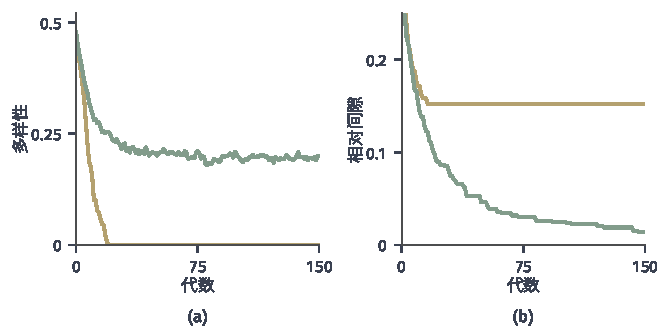
\includegraphics[width=112mm]{figures/05-optimization/05-stochastic-optimization/matplotlib/rs-ga-diversity/figure.pdf}
 \caption{$40$件物品的背包问题，$31$次运行的中位数。黄线不变异，绿线变异率$1/40$。(a)种群多样性，即两个不同成员平均相差的位数占总位数的比例。(b)历史最好可行解与最优价值的相对间隙，最优价值由动态规划算出。}
 \label{fig:rs-ga-diversity}
\end{BookInlineFigure}

保持多样性的手段有三个：变异持续注入新内容；较大的种群让位点的多样性丢失得慢；种群收敛后保留最好记录并重启。它们都消耗评价次数，要在预算内权衡。

精英保留也不能提供有限预算下的全局保证。它只保证种群的最好值不变差，这和第~\ref{sec:rs-es-selection}节的结论相同，精英甚至可能加速多样性的丢失，因为它的片段被反复选中。

\section{粒子群}
\label{sec:rs-pso}

演化策略让分布移动，遗传算法重组编码。还有一种组织方式：让每个候选都带着速度在连续空间中移动，并记住自己和同伴到过的好位置。这称为\term{粒子群优化}（particle swarm optimization，PSO）。接下来要弄清：怎样利用已发现的位置引导移动，移动的幅度由什么控制？

可以把它想成一群人在雾中找谷底，每人记得自己到过的最低处，也听得到一些同伴报告的最低处。每一步他沿惯性继续走，同时被这两个记忆的方向拉一下。这个比喻只对应更新公式的结构，不能推出任何收敛性质。

\subsection{个人与群体记忆}
\label{sec:rs-pso-memory}

粒子的移动依赖记忆。这一小节的问题是：每个粒子要记住什么，同伴之间共享什么？

\paragraph{完整状态}
设有$N$个粒子，变量是$\bm{x}\in\mathbb{R}^n$。第$i$个粒子第$t$步的状态由四个量组成：
\begin{itemize}
 \item 位置$\bm{x}_i^{(t)}$：当前候选；
 \item 速度$\bm{v}_i^{(t)}$：上一步的位移，不是目标的导数；
 \item \term{个人最好位置}（personal best）$\bm{p}_i^{(t)}$：这个粒子到过的最好位置；
 \item \term{邻域最好位置}（neighborhood best）$\bm{g}_i^{(t)}$：指定邻域内各粒子的个人最好位置中最好的一个。
\end{itemize}
本节的$\bm{g}_i$是位置，不是梯度。

初始化时在搜索区域内均匀抽位置，抽较小的初速度，评价一遍，令$\bm{p}_i^{(0)}=\bm{x}_i^{(0)}$，然后由定义得到$\bm{g}_i^{(0)}$。

个人记忆的更新规则是：
\begin{equation}
 \bm{p}_i^{(t+1)}=
 \begin{cases}
  \bm{x}_i^{(t+1)},&f(\bm{x}_i^{(t+1)})<f(\bm{p}_i^{(t)}),\\
  \bm{p}_i^{(t)},&\text{否则}.
 \end{cases}
 \label{eq:rs-pso-pbest}
\end{equation}
相同评价值时规定不更新，这样结果不依赖浮点上的偶然差别。在邻域内比较时，若有并列，按粒子编号取最小者，也要事先固定。

\paragraph{共享范围}
图~\ref{fig:rs-pso-topology}是两种共享方式。\textbf{全局共享}时所有粒子彼此相连，$\bm{g}_i$对所有$i$相同，就是全体个人记忆中最好的一个。\textbf{局部邻域}时每个粒子只与环上的相邻粒子交换信息，好位置要经过多步才能传遍全群。

\begin{BookInlineFigure}
 \centering
 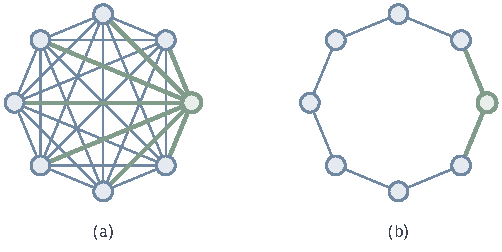
\includegraphics[width=85mm]{figures/05-optimization/05-stochastic-optimization/tikz/rs-pso-topology/figure.pdf}
 \caption{八个粒子的两种信息共享方式，绿色圆是当前关注的粒子，绿线是它能直接获知的同伴。(a)全局共享：每个粒子能看到其他所有粒子。(b)环形邻域：只与左右两个粒子交换。}
 \label{fig:rs-pso-topology}
\end{BookInlineFigure}

全局共享传播快，全群容易一起挤向同一个地方；环形邻域传播慢，不同区段可以暂时朝不同的好位置移动，保留较多的探索。

\paragraph{同步与异步}
实现上有两种顺序。\textbf{同步}更新时，一轮内所有粒子都用上一轮结束时的记忆移动，全部评价完再统一更新记忆，这便于并行评价。\textbf{异步}更新时，每评价完一个粒子，立即更新记忆，后面的粒子马上能用到新发现。两者的结果不同，记录算法时要写清楚用的是哪一种。下面用同步。

\subsection{速度与位置更新}
\label{sec:rs-pso-update}

有了状态和记忆，这一小节写出一步更新的公式，并按实际的次序算一遍。

\paragraph{主要思想}
新速度由三部分叠加：沿旧速度的惯性，朝个人记忆的拉力，朝邻域记忆的拉力。两个拉力的强度带随机性，以避免所有粒子沿同一条确定的轨迹运动：
\begin{equation}
 \begin{aligned}
 \bm{v}_i^{(t+1)}&=\bm{v}_i^{(t)}+c_1\bm{r}_{1}\odot\bigl(\bm{p}_i^{(t)}-\bm{x}_i^{(t)}\bigr)+c_2\bm{r}_{2}\odot\bigl(\bm{g}_i^{(t)}-\bm{x}_i^{(t)}\bigr),\\
 \bm{x}_i^{(t+1)}&=\bm{x}_i^{(t)}+\bm{v}_i^{(t+1)},
 \end{aligned}
 \label{eq:rs-pso-update}
\end{equation}
其中$c_1,c_2>0$是吸引系数，$\odot$表示按分量相乘，$\bm{r}_1,\bm{r}_2$的各个分量独立地均匀取自$[0,1]$，并且对每个粒子、每一轮重新抽取。

这里的差$\bm{p}_i-\bm{x}_i$和$\bm{g}_i-\bm{x}_i$只是到记忆位置的位移，不是目标的梯度。在下面的例子里$\bm{x}=(4,2)$，负梯度是$(-4,-18)$，朝邻域记忆的位移是$(-3,-1)$，两者的夹角约为$59^\circ$。粒子可以朝一个代价更高的方向飞，因为记忆里的点在那边。

\paragraph{变量}
一个粒子需要$\bm{x}$、$\bm{v}$、$\bm{p}$、$\bm{g}$，以及$f(\bm{p})$；全局还要保存历史最好记录。

\paragraph{初始化}
下面用$f(\bm{x})=\tfrac12(x_1^2+9x_2^2)$核对一步。设系数$c_1=c_2=1.5$，粒子当前状态是
\[
 \bm{x}=\begin{bmatrix}4\\2\end{bmatrix},\quad\bm{v}=\begin{bmatrix}-1\\0.5\end{bmatrix},\quad\bm{p}=\begin{bmatrix}3\\1\end{bmatrix},\quad\bm{g}=\begin{bmatrix}1\\1\end{bmatrix}.
\]
记忆处的代价是$f(\bm{p})=9$，$f(\bm{g})=5$。

\paragraph{每轮更新}
每一轮按下面的次序处理每个粒子，用完预算为止。

\begin{enumerate}
 \item 抽随机向量。例中
 \[
  \bm{r}_1=\begin{bmatrix}0.5\\0.2\end{bmatrix},\qquad\bm{r}_2=\begin{bmatrix}0.4\\0.6\end{bmatrix}.
 \]
 \item 由式~\eqref{eq:rs-pso-update}计算新速度。例中个人项和群体项分别是
 \[
  1.5\,\bm{r}_1\odot(\bm{p}-\bm{x})=\begin{bmatrix}-0.75\\-0.3\end{bmatrix},\qquad
  1.5\,\bm{r}_2\odot(\bm{g}-\bm{x})=\begin{bmatrix}-1.8\\-0.9\end{bmatrix},
 \]
 加上旧速度得到
 \[
  \bm{v}^{+}=\begin{bmatrix}-3.55\\-0.7\end{bmatrix}.
 \]
 \item 计算新位置并评价。例中
 \[
  \bm{x}^{+}=\begin{bmatrix}0.45\\1.3\end{bmatrix},\qquad f(\bm{x}^{+})=\tfrac12(0.2025+15.21)\approx7.71.
 \]
 \item 完成评价后更新记忆。例中$7.71<9$，个人记忆更新为$(0.45,1.3)$；$7.71>5$，邻域记忆$\bm{g}$不变。
\end{enumerate}

图~\ref{fig:rs-pso-vector}把这一步的三段位移画成首尾相接的箭头。这个粒子一步就把代价从$26$降到了约$7.71$，主要靠群体项。

\begin{BookInlineFigure}
 \centering
 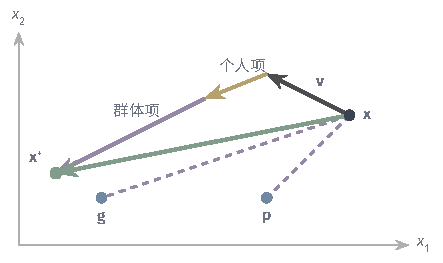
\includegraphics[width=75mm]{figures/05-optimization/05-stochastic-optimization/tikz/rs-pso-vector/figure.pdf}
 \caption{粒子的一步更新。深灰箭头是旧速度，黄箭头是个人项，紫箭头是群体项，绿箭头是合成的实际位移，虚线连向两个记忆位置。两个拉力分量的比例来自随机向量，所以合成位移不必指向任何一个记忆位置。}
 \label{fig:rs-pso-vector}
\end{BookInlineFigure}

\paragraph{速度限幅的计算}
实际常把速度各分量限制在$[-v_{\max},v_{\max}]$内。此时必须用修正后的速度计算位移。例中取$v_{\max}=2$，$\bm{v}^{+}$被截断为$(-2,-0.7)$，新位置是$(2,1.3)$，代价约为$9.61$。这比$f(\bm{p})=9$大，这一步个人记忆就不更新了。

记录下来的$\bm{v}^{+}$必须是截断后的那个，否则下一轮的惯性项与实际位移不一致。

图~\ref{fig:rs-pso-swarm}是二维Rastrigin函数上$24$个粒子的一次运行，三幅分别是第$0,8,60$轮的位置。第$8$轮粒子已聚向原点附近，第$60$轮已基本聚集，这次最好代价约为$2\times10^{-5}$。

\begin{BookInlineFigure}
 \centering
 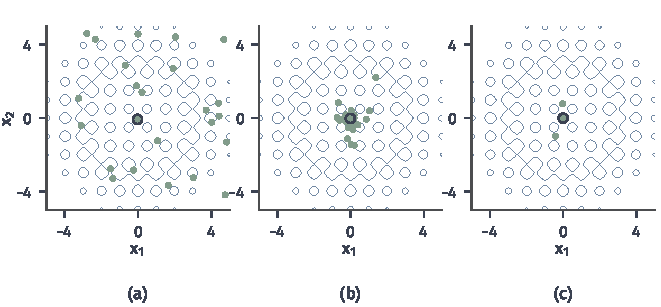
\includegraphics[width=112mm]{figures/05-optimization/05-stochastic-optimization/matplotlib/rs-pso-swarm/figure.pdf}
 \caption{二维Rastrigin函数上的粒子群，$N=24$，全局共享，带惯性权重$\omega=0.7298$，$c_1=c_2=1.496$，$v_{\max}=2$，同步更新，种子固定。(a)(b)(c)分别是第$0,8,60$轮的粒子位置（绿点），蓝线是等高线$f=30$，深色圆圈是当前的全局最好记忆，红点是全局最小点。}
 \label{fig:rs-pso-swarm}
\end{BookInlineFigure}

\subsection{移动尺度与停滞}
\label{sec:rs-pso-scale}

式~\eqref{eq:rs-pso-update}没有任何东西让速度变小。这一小节的问题是：什么控制粒子的移动尺度，粒子群停止移动时又说明了什么？

\paragraph{为什么要给速度加阻尼}
把问题简化。只看一维，记忆固定在$p=g=0$，把随机量换成常数，记$\varphi=c_1r_1+c_2r_2$。在旧速度前面乘上一个系数$\omega$（称为惯性权重），更新变成
\begin{equation}
 v^{+}=\omega v-\varphi x,\qquad x^{+}=x+v^{+}.
 \label{eq:rs-pso-deterministic}
\end{equation}
式~\eqref{eq:rs-pso-update}对应$\omega=1$。

\begin{theorem}[确定性粒子的稳定条件]
\label{thm:rs-pso-stability}
递推~\eqref{eq:rs-pso-deterministic}对任意初值都有$x^{(t)}\to0$，$v^{(t)}\to0$，当且仅当
\begin{equation}
 \lvert\omega\rvert<1,\qquad0<\varphi<2+2\omega.
 \label{eq:rs-pso-stable}
\end{equation}
\end{theorem}

\begin{proof}
把$v^{+}$代入第二式，$x^{+}=(1-\varphi)x+\omega v$，于是
\[
 \begin{bmatrix}x^{+}\\v^{+}\end{bmatrix}=\bm{M}\begin{bmatrix}x\\v\end{bmatrix},\qquad
 \bm{M}=\begin{bmatrix}1-\varphi&\omega\\-\varphi&\omega\end{bmatrix}.
\]
线性递推对任意初值收敛到零，当且仅当$\bm{M}$的两个特征值模都小于$1$。

$\bm{M}$的迹是$1-\varphi+\omega$，行列式是$\omega(1-\varphi)+\omega\varphi=\omega$，特征多项式为
\[
 \chi(z)=z^2-(1-\varphi+\omega)z+\omega.
\]

先计算两个端点的值：
\[
 \chi(1)=\varphi,\qquad\chi(-1)=2+2\omega-\varphi.
\]

两根为实数时，两根都在$(-1,1)$内，当且仅当$\chi(1)>0$，$\chi(-1)>0$，且两根之积的绝对值小于$1$，这三条合起来正是式~\eqref{eq:rs-pso-stable}。

两根为共轭复数时，$\omega>0$，模的平方等于乘积$\omega$，所以模小于$1$当且仅当$\omega<1$。此时判别式为负，给出
\[
 \lvert1-\varphi+\omega\rvert<2\sqrt{\omega}\leq1+\omega,
\]
这就是$0<\varphi<2+2\omega$，所以它自动成立。两种情形合起来，即得结论。
\end{proof}

$\omega=1$时行列式为$1$，两个特征值的模乘积为$1$，不可能都小于$1$，所以原始的式~\eqref{eq:rs-pso-update}没有衰减。图~\ref{fig:rs-pso-stability}(a)中$\omega=1$，$\varphi=1.5$的轨迹一直等幅振荡；$\omega=0.7$时振荡衰减，$45$步后已接近零。

这是把随机量换成常数后的结论，真实的$\varphi$每轮变化，乘积的稳定性与平均值的稳定性并不相同，定理只用来解释阻尼的作用。它说明了实践中必须做一件事：要么加$v_{\max}$，要么取$\omega<1$，否则粒子会越飞越散。

\begin{BookInlineFigure}
 \centering
 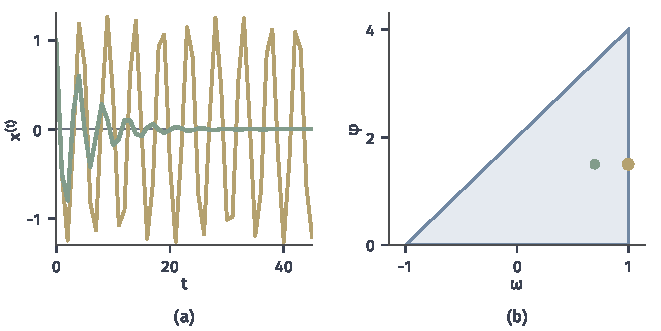
\includegraphics[width=112mm]{figures/05-optimization/05-stochastic-optimization/matplotlib/rs-pso-stability/figure.pdf}
 \caption{确定性粒子~\eqref{eq:rs-pso-deterministic}，记忆在原点，$x^{(0)}=1$，$v^{(0)}=0$。(a)$\varphi=1.5$，黄线$\omega=1$，绿线$\omega=0.7$。(b)蓝色三角形是稳定区域~\eqref{eq:rs-pso-stable}，两个点对应(a)中的两组参数，黄点位于边界上。}
 \label{fig:rs-pso-stability}
\end{BookInlineFigure}

\paragraph{三个控制量}
表~\ref{tab:rs-pso-controls}比较影响移动尺度和信息传播的三个量。它们的合适取值依赖问题和预算。

\begin{BookInlineTable}
 \centering
 \caption{粒子群的三个控制量。}
 \label{tab:rs-pso-controls}
 \begin{tabular}{lll}
  \toprule
  控制量 & 增大时 & 过度时 \\
  \midrule
  $v_{\max}$ & 允许跳得更远 & 粒子飞出搜索区域 \\
  $c_1,c_2$ & 向记忆靠拢更用力 & 振荡，越过记忆点 \\
  邻域大小 & 信息传播更快 & 全群过早聚到一处 \\
  \bottomrule
 \end{tabular}
\end{BookInlineTable}

\paragraph{越界的处理}
粒子飞出搜索区域$[\ell_j,u_j]$时，位置和速度都要处理。常用的做法是把位置截断到边界并把该分量速度置零，或者把位置反射回来并反转速度分量。

只截断位置、保留原速度是不行的：下一步粒子会继续往外冲，每一轮都贴在边界上。不管用哪一种，都要保证下一轮的$\bm{v}$与实际位移一致，这一点和速度限幅相同。第~\ref{sec:rs-constraints}节会说明，这些处理也改变了搜索的分布。

\paragraph{停滞}
考虑这样的状态：全体粒子都位于同一点$\bm{x}^\circ$，$\bm{p}_i=\bm{g}_i=\bm{x}^\circ$，$\bm{v}_i=\bm{0}$。代入式~\eqref{eq:rs-pso-update}，两个差都是零，旧速度也是零，于是不论$\bm{r}_1,\bm{r}_2$取什么值，
\[
 \bm{v}_i^{+}=\bm{0},\qquad\bm{x}_i^{+}=\bm{x}^\circ.
\]
算法从此不再移动。

这个$\bm{x}^\circ$可以是任何点。比如在$f=\tfrac12(x_1^2+9x_2^2)$上，$\bm{x}^\circ=(1,1)$的梯度是$(1,9)$，它连驻点都不是。所以粒子聚在一起、速度趋于零或者记录长期不变，都只是搜索过程的描述，不是最优性的证明。

实际运行中粒子不一定精确聚在一点，但速度变小后移动的尺度已不足以发现更好的位置，效果相同。常用的补救是重新分散一部分粒子，同时保留历史最好记录。

\section{约束处理}
\label{sec:rs-constraints}

前面几节的手算例子已经遇到了不可行的候选：背包问题里超重的串，排列交叉产生的重复元素，粒子飞出区域。这就需要回答：候选不可行时有哪些处理方式，每种方式实际上交出了什么解，又对搜索分布有什么影响？

\paragraph{先判断可行}
处理之前要能回答“这个候选在不在$\bm{C}$里”。问题~\eqref{eq:rs-problem}的$\bm{C}$通常由判定条件给出：盒约束逐分量比较上下界，排列检查元素是否恰好各出现一次，背包约束把重量加起来和容量比较。

如果判定本身需要昂贵的模拟，每次判定也要计入预算。若只有$f$的评价能告诉我们是否可行，可行性就成了评价信息的一部分。

\paragraph{直接在可行集中产生候选}
第一种方式是让操作本身不产生不可行的候选：排列上用交换和顺序交叉，盒内均匀初始化。这是最干净的做法，所有评价都用在可行候选上，不需要额外的规则。它的限制是这样的操作不总存在，一般的约束集合上没有简单的抽样办法。

\paragraph{拒绝}
第二种方式是把不可行提议直接丢弃，就当没发生，等价于把不可行候选的代价设为$+\infty$。模拟退火中，拒绝后留在原地，提议的对称性不受影响，定理~\ref{thm:rs-detailed-balance}的结论在$\bm{C}$上仍然成立，平稳分布是限制在可行集上的Gibbs分布。

代价是可行集很小时大部分提议都浪费了，并且可行集不连通时，由邻域提议连接起来的图可能分成几块，算法走不到另一块。是否花费评价次数取决于是否在判定前做函数评价，这一点要照实计入。

\paragraph{修复}
第三种方式是把不可行候选映射成一个可行候选，再评价。盒约束常用的是截断和反射；背包问题可以按价值密度$v_j/w_j$从低到高去掉物品，直到重量合格。

用遗传算法一节的不可行串$110110$演示。选中的物品是$1,2,4,5$，价值密度依次是$3$，$1.67$，$1.29$，$1.2$。去掉第$5$件后总重$12$，不超容量，得到$110100$，$f=-20$。

这时要明确记录什么。评价的是修复后的$110100$，交出去的、记入最好记录的也必须是$110100$，而不是原来的串。种群中可以存修复后的串，也可以存原串但使用修复后的评价，两种规则都可以，但要事先选定。

排列也可以修复。遗传算法一节非法的$12524$里元素$2$重复、元素$3$缺失，把第二次出现的$2$改成$3$，得到合法排列$12534$。修复规则不唯一，用哪条规则也要写明。

\paragraph{修复会改变搜索分布}
修复不是无害的。图~\ref{fig:rs-box-repair}(a)是一维的例子，当前点$x=0.1$，提议$\mathcal{N}(0.1,0.3^2)$，可行集为$[0,1]$。落到区间外的概率约$0.37$。截断把这些概率全部堆到边界$0$这一点，形成一个集中的质量；反射把区间外的部分折回区间内，密度连续；拒绝则把这部分质量留在当前点。

对称性是否保留是关键。反射后的提议密度是
\[
 \tilde q(x,y)=\sum_{k\in\mathbb{Z}}\bigl[\phi(y-x+2k)+\phi(y+x+2k)\bigr],
\]
其中$\phi$是$\mathcal{N}(0,0.3^2)$的密度。它关于$x,y$对称，所以模拟退火可以沿用式~\eqref{eq:rs-metropolis}。截断不具有这个性质。

\begin{BookInlineFigure}
 \centering
 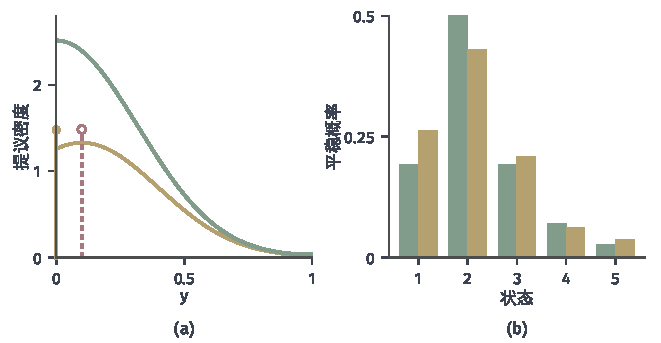
\includegraphics[width=112mm]{figures/05-optimization/05-stochastic-optimization/matplotlib/rs-box-repair/figure.pdf}
 \caption{修复对分布的影响。(a)从$x=0.1$出发的提议$\mathcal{N}(0.1,0.3^2)$在$[0,1]$上的三种处理：黄线是截断后区间内的密度，黄色竖线是截断堆积在$0$处的质量（高度为质量的$4$倍）；绿线是反射后的密度；红色虚线是拒绝时留在$x=0.1$的质量（同样放大$4$倍）。(b)五状态链的平稳分布，绿柱为Gibbs分布，黄柱是用截断提议而未修正接受概率时的实际平稳分布。}
 \label{fig:rs-box-repair}
\end{BookInlineFigure}

用离散的例子算一下。状态$\{1,\ldots,5\}$，代价$f=(1,0,1,2,3)$，$T=1$。提议从$\{-2,-1,+1,+2\}$等概率选步，超出范围就截断到端点。从$2$往左：$-1$到$1$，$-2$截断也到$1$，所以
\[
 q(2,1)=\frac12,\qquad q(1,2)=\frac14,
\]
提议不再对称。

仍用式~\eqref{eq:rs-metropolis}，实际的平稳分布约为$(0.262,0.430,0.208,0.063,0.037)$，而目标的Gibbs分布约为$(0.192,0.521,0.192,0.070,0.026)$，见图~\ref{fig:rs-box-repair}(b)。最优状态$x=2$的概率从$0.521$掉到$0.430$，边界状态的概率被抬高了。

要恢复Gibbs分布，须改用式~\eqref{eq:rs-hastings}的修正接受概率。因此模拟退火一旦带修复，就要重新核对提议与接受规则，第~\ref{sec:rs-sa-barrier}节的定理也不能直接引用。遗传算法、粒子群没有平稳分布的目标，修复的影响表现为搜索偏向边界。

\paragraph{惩罚评价}
第四种方式是把违反量折算成代价。设违反量$V(\bm{x})\geq0$，$V(\bm{x})=0$当且仅当可行，搜索时比较
\begin{equation}
 f_\rho(\bm{x})=f(\bm{x})+\rho V(\bm{x}),\qquad\rho>0.
 \label{eq:rs-penalty}
\end{equation}

系数要足够大才有用。背包问题中$V$取超重量，串$110110$的$f=-26$，$V=2$。取$\rho=1$，$f_1=-24$，低于最优可行解的$-23$，搜索会认为这个不可行的串是最好的。取$\rho=10$时是$-6$，它就排到了后面。

但$\rho$过大时，惩罚值的量级盖过$f$的差别，可行边界附近的比较失去区分度。这一取舍的系统讨论见第~\ref{chap:penalty-multiplier-methods}章。

无论$\rho$取多少，最好记录都要按式~\eqref{eq:rs-best-record}只在可行候选上更新。交出的结果若$V>0$，就要明确说明，不能和可行解的代价放在一起比较。

\paragraph{四种方式的比较}
表~\ref{tab:rs-constraints}汇总了各种方式，重点是实际返回的解。

\begin{BookInlineTable}
 \centering
 \caption{约束处理方式的比较。}
 \label{tab:rs-constraints}
 \begin{tabular}{lll}
  \toprule
  方式 & 返回的解 & 主要风险 \\
  \midrule
  可行内生成 & 原候选 & 适用的集合有限 \\
  拒绝 & 原候选 & 浪费提议，可行集分块 \\
  修复 & 修复后的候选 & 改变搜索分布 \\
  惩罚 & 原候选，须核查可行性 & 系数不当，交出不可行解 \\
  \bottomrule
 \end{tabular}
\end{BookInlineTable}

这些都是搜索算法层面的工程处理，只回答“候选不可行时算法怎么办”。约束的最优性条件、乘子和一般的约束算法由第~\ref{chap:constrained-optimality}章起的第六部分承担。


\section{含噪评价}
\label{sec:rs-noise}

到目前为止，读数都等于真实代价。如果每次评价带有噪声，如式~\eqref{eq:rs-reading}，同一个候选评价两次也会得到不同的数。噪声影响了算法的哪些环节，最好记录的含义变成了什么，额外的评价应当花在哪里？

\paragraph{噪声影响三个环节}
先明确优化的对象。本节设读数误差$\varepsilon$的均值为零，要最小化的是期望代价$f(\bm{x})=\mathbb{E}[\tilde f(\bm{x})]$；如果关心的是分位数或最坏情形，要先改定目标。这也说明，第~\ref{sec:rs-sa-barrier}节的定理和第~\ref{sec:rs-es-selection}节的单调性都是针对精确代价的，不能直接用到含噪读数上。

第一个受影响的是\textbf{接受}。设真实上坡量为$2$，$T=0.5$，无噪声时接受概率为$\mathrm{e}^{-4}\approx0.018$。若两次读数的误差各自服从$\mathcal{N}(0,1)$，接受概率的平均值变成约$0.157$，是原来的八倍多。噪声的效果相当于抬高了温度。

第二个是\textbf{排序}：种群中的名次可能和真实好坏相反，选择压力被噪声稀释。第三个是\textbf{最好记录}，这是最隐蔽的，下面专门讨论。

\paragraph{最低读数偏向有利噪声}
设有$N$个候选，真实代价都是$0$，读数相互独立，服从$\mathcal{N}(0,1)$。算法把读数最低的那个当作最好解，它的读数是$N$个标准正态变量的最小值，期望是负的。

$N=2$时可以手算。由$\min(a,b)=\tfrac12(a+b-\lvert a-b\rvert)$，两个读数$Z_1,Z_2$的最小值的期望是
\[
 \mathbb{E}\min(Z_1,Z_2)=-\tfrac12\mathbb{E}\lvert Z_1-Z_2\rvert.
\]

$Z_1-Z_2\sim\mathcal{N}(0,2)$，$\mathbb{E}\lvert Z\rvert=\sqrt{2/\pi}$，于是
\[
 \mathbb{E}\min(Z_1,Z_2)=-\tfrac12\cdot\sqrt2\cdot\sqrt{\frac2\pi}=-\frac{1}{\sqrt\pi}\approx-0.564.
\]

$N$增大，这个偏差继续变大。图~\ref{fig:rs-noise-selection}(a)显示$N=1000$时最低读数的均值约为$-3.24$，虽然所有候选的真实代价都是$0$。比较的次数越多，“最好”的读数越乐观。

\begin{BookInlineFigure}
 \centering
 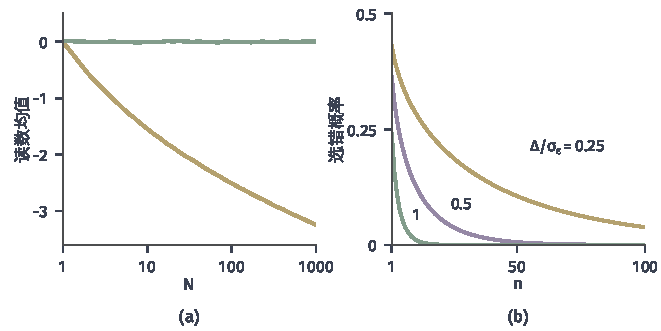
\includegraphics[width=112mm]{figures/05-optimization/05-stochastic-optimization/matplotlib/rs-noise-selection/figure.pdf}
 \caption{噪声下的选择。(a)$N$个真实代价都为$0$的候选，噪声服从$\mathcal{N}(0,1)$，黄线是最低读数的均值，绿线是对选出者重新读一次的均值，由$20000$次抽样估计。(b)两候选真实差为$\Delta$，噪声标准差为$\sigma_\varepsilon$，各读$n$次后按样本均值选错的概率，按式~\eqref{eq:rs-wrong-selection}计算。}
 \label{fig:rs-noise-selection}
\end{BookInlineFigure}

\subsection{候选比较}
\label{sec:rs-noise-compare}

两个候选的读数不同，这个差别是真的吗？这一小节讨论要读多少次才能下判断，以及读数应当分给谁。

\paragraph{重复读数}
设候选$\bm{a}$的真实代价比$\bm{b}$低$\Delta>0$。每个候选独立读$n$次，取样本均值。读数的噪声方差都是$\sigma_\varepsilon^2$时，样本均值之差的方差是$2\sigma_\varepsilon^2/n$。

样本均值之差的标准差按$1/\sqrt{n}$下降，而要分辨的真实差$\Delta$不变，所以$\Delta$越小，需要的读数越多。

\begin{theorem}[两候选比较的错误概率]
\label{thm:rs-comparison}
设两候选的读数相互独立，方差都是$\sigma_\varepsilon^2$，真实代价差为$\Delta>0$，各读$n$次后选样本均值较低者。若噪声服从高斯分布，选错的概率为
\begin{equation}
 \mathbb{P}(\text{选错})=\Phi\Bigl(-\frac{\Delta}{\sigma_\varepsilon}\sqrt{\frac{n}{2}}\Bigr),
 \label{eq:rs-wrong-selection}
\end{equation}
其中$\Phi$是标准正态分布函数。若只假定方差有限，则有
\begin{equation}
 \mathbb{P}(\text{选错})\leq\frac{2\sigma_\varepsilon^2}{n\Delta^2}.
 \label{eq:rs-wrong-chebyshev}
\end{equation}
\end{theorem}

\begin{proof}
记$\bar{a},\bar{b}$为两个样本均值，令$W=\bar{a}-\bar{b}+\Delta$，$W$的均值为$0$，方差为$2\sigma_\varepsilon^2/n$。选错即$\bar{a}\geq\bar{b}$，也就是$W\geq\Delta$。

高斯情形下$W\sim\mathcal{N}(0,2\sigma_\varepsilon^2/n)$，标准化后即得式~\eqref{eq:rs-wrong-selection}。方差有限时，由Chebyshev不等式，
\[
 \mathbb{P}(W\geq\Delta)\leq\mathbb{P}(\lvert W\rvert\geq\Delta)\leq\frac{2\sigma_\varepsilon^2}{n\Delta^2}.
\]
\end{proof}

图~\ref{fig:rs-noise-selection}(b)是式~\eqref{eq:rs-wrong-selection}。$\Delta/\sigma_\varepsilon=1$时，一次读数选错的概率约为$0.24$，$n=4$时约为$0.079$，$n=16$时约为$0.002$。$\Delta/\sigma_\varepsilon=0.5$时要$n=16$才降到$0.079$，差减半，读数要多四倍。这也就是说，$n$按$(\sigma_\varepsilon/\Delta)^2$增长。

方差未知时要用样本方差，置信水平还要计入同时比较的次数，这些统计保证的条件和推导可参考\BookChapterRef{chap:finite-sample-error-bounds}{卷八第4章“有限样本的误差上界”}。

\paragraph{把预算分给难分辨的候选}
候选的差别悬殊时，一两次读数就够分辨；差别小的，才值得多读。因此比全体平均分配读数更省的安排是：先给每个候选少量读数，计算均值和不确定性区间，淘汰区间明显落后的候选，把后续读数分给仍难分辨的那些。

这里要区分两种错误。比较误差是已见候选之间排错了名次；覆盖不足是更好的点根本没被评价过。多读几次已见的候选，只能减少前者。复核已见候选不能证明不存在更优的未见点。用于复核的读数和探索新候选竞争同一份预算，两者的分配要依问题决定。

\subsection{历史最好解的复核}
\label{sec:rs-noise-reeval}

上面看到最低读数偏向有利噪声。这一小节的问题是：对选出来的候选还能相信什么，要怎样复核？

\paragraph{选中之后重新评价}
式~\eqref{eq:rs-best-record}的记录是一次选择的结果，所以这个读数带偏。对选出的候选\textbf{用新的独立读数}重新评价，得到的就是无偏的估计。

原因是：选择只依赖旧的读数，新的噪声与选择无关。设选中的候选是$\hat{\bm{x}}$，给定$\hat{\bm{x}}$的条件下，新读数的条件期望是$f(\hat{\bm{x}})$，所以
\begin{equation}
 \mathbb{E}\bigl[\tilde f_{\mathrm{new}}(\hat{\bm{x}})\mid\hat{\bm{x}}\bigr]=f(\hat{\bm{x}}).
 \label{eq:rs-fresh-reading}
\end{equation}
图~\ref{fig:rs-noise-selection}(a)的绿线正是这一点，重新读一次的均值稳定在真实值$0$附近。

条件是新读数必须与用于选择的读数独立。把旧读数和新读数平均，偏差只是减小，并不消失。若一批复核读数又用来在多个候选中再选一次，新的选择偏差又产生了，要再留一批读数来做最终的估计。

\paragraph{新旧记录的比较}
旧记录的读数是经过多次比较选出来的最小值，新候选只有一次读数，两者并不能等量比较。$(1+1)$策略一旦遇到一次特别幸运的读数，后代的一次读数几乎都比不过它，这个亲代就长期占位，算法看起来“收敛”了，实际只是被一次噪声卡住。

常用的修正是每一代重新评价亲代，或者让记录中的候选累积多次读数后再参与比较。这些额外的评价都要计入预算，代价是每代评价数增加。

\paragraph{要记录什么}
搜索过程实际使用的选解规则要原样记录：是取最低的单次读数，还是取重复读数的最低均值，还是另留一批独立读数做最后的裁决。

报告结果时也要说清每个数字的来源。“最好值”如果是搜索过程中的最低读数，就是偏乐观的；如果来自独立的复核读数，才能作为对$f(\hat{\bm{x}})$的估计。样本复用省评价次数，但信息依赖也要一并交代。

\section{结果评价}
\label{sec:rs-evaluation}

前面每种方法都给出了手算和几幅运行图。于是要问：两种随机搜索的结果怎样比才算数，一次运行结束时能下什么结论？要把三类说法分开：有限预算内得到了什么，长期运行有什么极限性质，以及能否验证结果确实接近最优。

\subsection{停止条件}
\label{sec:rs-eval-stop}

算法要在某一刻停下来。这一小节的问题是：各种停止规则分别支持什么结论？

\paragraph{四种规则}
\textbf{评价次数上限}在用完$B$次后停止，这是最容易比较的一种。\textbf{时间上限}在规定的墙钟时间后停止，它依赖机器和实现。\textbf{目标阈值}在$f_{\mathrm{best}}\leq f_{\mathrm{target}}$时停止，要有事先给定的阈值。\textbf{停滞规则}在连续若干轮没有改善时停止。

\paragraph{停滞规则只描述已观察到的过程}
图~\ref{fig:rs-eval-budget}(c)是五维Rastrigin问题上遗传算法的一次运行。最好值从第$300$次评价前后开始，在$10.28$上停了$500$多次评价，接着又下降，最后约为$0.02$。若规则是“连续$500$次评价没有改善就停”，这次运行就会在那段平台上结束，报告$10.28$。

停滞规则说的是最近没有发现更好的点，不代表不存在更好的点。它是预算的管理手段，不是最优性的判据。分布的$\sigma$变小、粒子聚集、种群趋同也都一样。

\paragraph{有下界时报告间隙}
能证明$\ell\leq f^\star$时，可行解$\hat{\bm{x}}$的目标差不超过$f(\hat{\bm{x}})-\ell$，这是可以验证的结论，第~\ref{chap:optimization}章讨论过这种夹逼。

第~\ref{sec:rs-ga}节的背包问题就是如此：把物品按价值密度排序，允许最后一件取一部分，得到的分数背包最优值是原问题价值的上界，也就是代价的下界。那里的六件物品按价值密度排序，取第$1,2,3$件用去重量$11$，再取第$4$件的$4/7$，分数解的总价值为$19+\tfrac47\times9\approx24.14$。价值都是整数，所以$f^\star\geq-24$，最好可行解$-23$与最优值至多差$1$，这是不依赖搜索过程的结论。

大多数黑箱问题没有可靠的下界。这时老实的报告是：最好可行值是多少，用了多少次评价。不能写“达到全局最优”，因为最优值未知，而$f(\hat{\bm{x}})-f^\star$根本无从计算。

\subsection{预算与重复运行}
\label{sec:rs-eval-budget}

停下来以后要比较。这一小节的问题是：不同算法的成本怎样折算到同一单位，一次运行不够时要比较什么？

\paragraph{统一的成本单位}
不同算法的“一轮”含义不同：退火的一轮是一次评价，CMA-ES的一代是$\lambda$次，粒子群的一轮是$N$次。按轮数比较没有意义，必须换算成实际的函数调用次数。表~\ref{tab:rs-cost-accounting}列出需要计入的内容。

\begin{BookInlineTable}
 \centering
 \caption{成本的记录。第一类按评价次数统一累计，第二类另行报告。}
 \label{tab:rs-cost-accounting}
 \begin{tabular}{ll}
  \toprule
  类别 & 项目 \\
  \midrule
  函数调用 & 种群评价、退火尝试、修复后的评价 \\
  & 重复读数、最好解复核、重启 \\
  & 温度标定等试探性评价 \\
  \midrule
  内部运算 & CMA-ES的矩阵分解、排序 \\
  存储 & 种群、协方差矩阵、记忆位置 \\
  并行 & 群体通信、同步等待的时间 \\
  \bottomrule
 \end{tabular}
\end{BookInlineTable}

评价便宜时，内部运算可能反而占主导，这时只数评价次数是不够的；评价昂贵时，内部运算可以忽略。两者都要记下，分别报告。

\paragraph{结果是一个分布}
这些算法是随机的，一次运行的结果只是一个样本。比较时要固定问题、固定初始条件的抽取规则和预算，做若干次独立运行，比较结果的分布，例如中位数和四分位数。用一次最好的运行代表一个方法，或者挑选种子，都没有意义。

\paragraph{比较实验}
图~\ref{fig:rs-eval-budget}比较五种做法。问题是五维Rastrigin函数，搜索区域为$[-5.12,5.12]^5$，统一预算$B=10000$，每种方法独立运行$41$次。表~\ref{tab:rs-eval-summary}给出结束时的结果，“达标”指最好值不超过$3$。

\begin{BookInlineFigure}
 \centering
 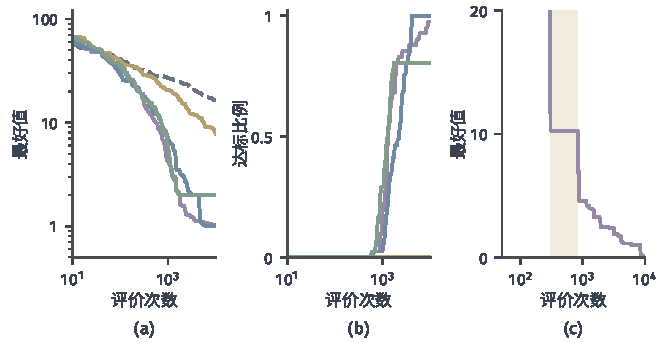
\includegraphics[width=112mm]{figures/05-optimization/05-stochastic-optimization/matplotlib/rs-eval-budget/figure.pdf}
 \caption{五维Rastrigin函数上的比较，$B=10000$，每种方法$41$次独立运行。灰色虚线为均匀随机抽样，黄线为模拟退火，紫线为实数编码遗传算法，蓝线为粒子群，绿线为CMA-ES。(a)最好值中位数随评价次数的变化。(b)最好值不超过$3$的运行所占比例。(c)遗传算法一次运行的最好值，浅黄区间是一段长约$530$次评价没有改善的平台。}
 \label{fig:rs-eval-budget}
\end{BookInlineFigure}

\begin{BookInlineTable}
 \centering
 \caption{$B=10000$时的结果（$41$次运行）。}
 \label{tab:rs-eval-summary}
 \begin{tabular}{lrrr}
  \toprule
  方法 & 中位数 & 上下四分位 & 达标比例 \\
  \midrule
  均匀随机抽样 & $16.49$ & $13.84$--$18.49$ & $0$ \\
  模拟退火 & $7.86$ & $5.69$--$10.35$ & $0$ \\
  遗传算法 & $1.03$ & $0.11$--$2.00$ & $0.98$ \\
  粒子群 & $0.99$ & $0.99$--$1.28$ & $1.00$ \\
  CMA-ES & $1.99$ & $0.99$--$2.98$ & $0.80$ \\
  \bottomrule
 \end{tabular}
\end{BookInlineTable}

这张表说明什么、不说明什么要说清楚。在这个问题、这组未专门调参的设置、这个预算下，三种基于群体或分布的方法达到了相近的量级，均匀抽样和这里的单点退火明显落后。

它不说明任何方法“更好”。退火换一组温度和提议尺度，结果可能大幅改变；CMA-ES此时已经收敛，后段的预算没有用上，加上重启可能改善；换一个问题，排序也可能颠倒。

图~\ref{fig:rs-eval-budget}(b)的曲线比一个终点数字更有信息：它回答了“要达到这个目标需要多少次评价”，三种方法都在约$10^3$次评价附近开始达标，CMA-ES的比例在约$0.8$处走平。

\paragraph{三类结论}
表~\ref{tab:rs-claims}把本章的结论按能够支持什么说法分类。写报告时，要清楚自己手里的结论属于哪一类。

\begin{BookInlineTable}
 \centering
 \caption{三类结论。}
 \label{tab:rs-claims}
 \begin{tabular}{ll}
  \toprule
  类别 & 例子与含义 \\
  \midrule
  有限预算的结果 & 中位数、达标比例：只对所测的设置成立 \\
  长期收敛结论 & 对数降温定理：是极限，并依赖模型条件 \\
  可验证的证书 & 下界与间隙：与算法如何运行无关 \\
  \bottomrule
 \end{tabular}
\end{BookInlineTable}

\section{本章小结}
\label{sec:rs-summary}

本章讨论只能评价候选时怎样组织搜索。局部改善会停在低谷，这在有限状态的双谷代价和二维多峰函数上都看得很清楚。要越过障碍，算法必须做眼前并不划算的事，四类方法的差别在于保存什么、用什么规则更新。

\textbf{模拟退火}控制单个状态的接受。对称提议下，固定温度的接受规则使Gibbs分布平稳。全局收敛定理只在有限状态、提议连通且$c\geq d^\star$的对数降温下成立，而且是概率的极限。实际的几何降温按有限预算的结果评价，温度要与代价的尺度匹配。

\textbf{演化策略}适应变异分布。保留亲代使最好值不增，整代替换允许当前值上升。CMA-ES用选中后代的加权平均移动中心，用路径和选中位移更新协方差，用标准化路径的长度调整尺度。搜索协方差不是Hessian，也不无条件等于Hessian的逆。高斯搜索分布的均值梯度与第~\ref{chap:zeroth-order-optimization}章的平滑梯度估计重合，排序效用则改变了目标。

\textbf{遗传算法}组织编码的重组与替换。编码决定什么叫邻近，排列上要用保持排列的算子，比例选择要先把代价转换为非负权重。交叉重组已有片段，变异引入新内容，没有变异时种群会完全趋同。

\textbf{粒子群}利用个人和邻域的记忆移动候选。记忆的差不是梯度，没有阻尼时确定性粒子不衰减，速度限幅后要按修正后的速度计算位移。粒子聚在一起不是最优性的证明。

各种方法要落在同一套可行性、评价信息和预算的记账上。不可行候选的处理决定了实际返回的解，修复会改变搜索分布，模拟退火须重新核对接受规则。含噪读数下最低读数偏向有利噪声，对选出的候选要用独立的新读数复核。比较方法时按实际函数调用统一预算，比较多次独立运行的结果分布。

搜索取得改善，不等于找到了全局最优。能给出下界时报告间隙，否则如实报告最好可行值和所用的预算。下一章讨论评价更昂贵的情形，用概率代理模型决定下一次评价的位置。


\chapter{贝叶斯优化}
\label{chap:bayesian-optimization}

一次流体仿真要跑四个小时，它有一个需要调节的参数，我们希望输出误差尽量小。仿真程序是一个不透明的黑箱，给它一个参数，它还回一个数，不给导数。这周的算力只够运行六次。第六次运行结束时必须交出一个参数值，往后就按它使用。六次机会应该怎么花？

第~\ref{chap:zeroth-order-optimization}章用函数值差分构造局部方向，第~\ref{chap:random-search}章靠大量候选的提议和淘汰探索解空间，这两条路都假定评价次数可以比较多。评价极贵时，每一次评价之后都值得停下来，把已有读数全部用上，认真想一想下一次该放在哪里。\term{贝叶斯优化}（Bayesian optimization）就是把这件事组织成计算的办法：用已完成的读数建立一个带不确定性的概率模型，再按潜在收益和不确定性决定下一次评价。

全章用一个一维仿真例子贯穿。我们先说清问题里“评价点”和“最终推荐”的区别，再建立高斯过程这个概率模型，然后比较几种把模型变成选点分数的规则，把它们接成一个完整的循环。之后依次放宽理想假设，讨论读数有噪声、约束也要试验才知道、多个试验同时运行三种情形。最后回答预算怎样核算，最终结果怎样评价，以及哪些结论有理论保证、在什么条件下成立。

\section{昂贵黑箱问题}
\label{sec:bo-problem}

只有$T$次昂贵评价时，优化问题应当怎样提？设搜索域$\bm{C}\subseteq\mathbb{R}^n$已知，目标$f:\bm{C}\to\mathbb{R}$的表达式未知，要解的是
\begin{equation}
 \min_{\bm{x}\in\bm{C}}\ f(\bm{x}),
 \label{eq:bo-problem}
\end{equation}
其中每次只能选一个$\bm{x}$，付出一次运行的代价，读到一个函数值。这类只能通过读数了解目标的问题称为\term{黑箱优化}（black-box optimization）。

与前面各章不同，这里最先固定的不是精度，而是预算：允许多少次评价，或者总共多少运行时间。问题随之变成“这$T$次机会怎样分配”。机会要分给两类地方：看起来有希望的区域，以及几乎一无所知的区域。只去前者可能错过别处更深的谷，只去后者又用不上已经学到的东西。

\paragraph{贯穿全章的例子}
设仿真参数$x$在$\bm{C}=[0,8]$内取值，输出误差$f(x)$已作标准化，负值表示比基准好，预算$T=6$。表~\ref{tab:bo-readings}列出整数位置上的读数。真实计算时这张表并不存在，算法只会知道被评价过的那几列；把它写出来是为了让后面的每一步都可以核对。

\begin{BookInlineTable}
 \centering
 \caption{贯穿例的整数位置读数。函数$f$是过这九个点的自然三次样条，只作为教学假设，算法不知道它。}
 \label{tab:bo-readings}
 \begin{tabular}{cccccccccc}
 \toprule
 $x$&0&1&2&3&4&5&6&7&8\\
 \midrule
 $f(x)$&0.9&0.2&$-0.5$&0.1&0.7&0.3&$-1.0$&$-0.3$&0.8\\
 \bottomrule
 \end{tabular}
\end{BookInlineTable}

这个函数有两个谷，一个在$x=2$附近，另一个在$x=6$附近，后者更深。样条的最小值约为$-1.029$，在$x\approx6.13$处取得。

\subsection{评价点与推荐解}
\label{sec:bo-query-recommend}

六次评价结束后要交出一个答案。答案未必是读数最好的那次，也未必是评价过的点。为了不把两件事混在一起，需要分开两个角色：\emph{评价点}用来收集信息，\emph{推荐解}用来实际采用。

图~\ref{fig:bo-query-recommend}是后面算法在贯穿例上实际走出的六次评价，数字是评价的先后。第$4$次去了$x=8$，读数$0.8$很差，从目标值看是一次失败。可是它告诉我们右端不值得再投入，这对后面的判断有用。第$5$次在$x=6$读到$-1.0$，于是最终推荐$\widehat{x}_6=6$。第$6$次在$x=0$的读数$0.9$又差得多，但这并不影响推荐，因为推荐解不需要是最后一次评价。

\begin{BookInlineFigure}
 \centering
 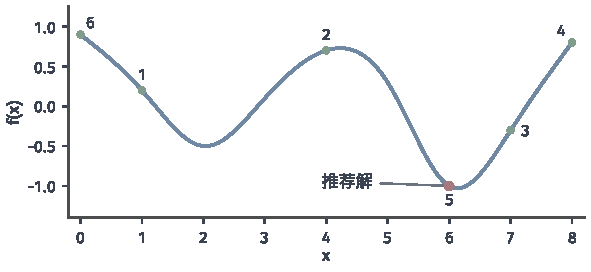
\includegraphics[width=100mm]{figures/05-optimization/05-stochastic-optimization/matplotlib/bo-query-recommend/figure.pdf}
 \caption{评价点与推荐解。蓝线是目标$f$，绿点是六次评价，旁边的数字是评价顺序，红点是最终推荐。第$4$次和第$6$次的读数很差，它们的任务是收集信息，不是交付答案。}
 \label{fig:bo-query-recommend}
\end{BookInlineFigure}

用数据集合记录当前已有的信息。设前$t$次评价的位置与读数为$(\bm{x}_i,y_i)$，记
\begin{equation}
 \mathcal{D}_t=\{(\bm{x}_i,y_i)\}_{i=1}^t.
 \label{eq:bo-data}
\end{equation}
这里下标$i$表示第$i$次评价，因为后面总要同时引用多次评价的位置，所以本章把评价序号写在下标。

选点规则必须遵守时间次序：第$t+1$个评价点只能依赖$\mathcal{D}_t$，至多再加上与目标无关的随机数，不能用尚未返回的读数。图~\ref{fig:bo-info-timeline}画出了这个次序。这条要求看似多余，实际很有约束力。比较不同方法时，若某个方法的超参数是用全部读数调好的，它在前几步就已用到了未来的信息，比较便不公平。

\begin{BookInlineFigure}
 \centering
 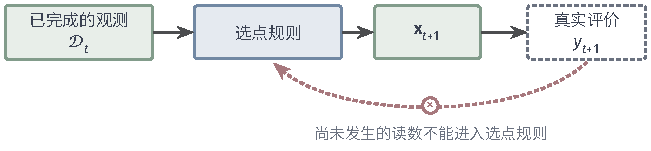
\includegraphics[width=110mm]{figures/05-optimization/05-stochastic-optimization/tikz/bo-info-timeline/figure.pdf}
 \caption{选点规则可以使用的信息。选点规则只读取已完成的观测$\mathcal{D}_t$，下一次评价的读数$y_{t+1}$在选点之后才产生（虚线框），红色虚线表示这条信息通路不允许存在。}
 \label{fig:bo-info-timeline}
\end{BookInlineFigure}

\subsection{概率模型的作用}
\label{sec:bo-probability-role}

只有三个读数时，$x=6$处的函数值是多少？我们不知道，但并非毫无看法：离读数近的地方函数值大概与读数接近，离得远的地方拿不准。要把“大概”和“拿不准”写成可以计算的东西，需要给未知的$f$配一个概率描述。

这里最容易误解的一点是，$f$本身并不随机。仿真程序是确定的，同一个$x$每次算出同样的结果，只是我们不知道结果。概率描述的是我们的认识状态，不是目标的物理性质。做法是引入一个随机函数$F$作为模型，把$f$看成它可能的一种情形。在看到数据之前，$F$的分布称为\term{先验}（prior）；把$\mathcal{D}_t$作为条件之后，$F$的分布称为\term{后验}（posterior）。

后验分布的变化，表示认识变了，不表示目标变了。可以把它想成一张还在绘制中的地形图：实地地形一直没动，测过的点清晰，没测过的地方模糊，每多测一点，图就清楚一些。这个比方有一处不准确：地形图的模糊只来自没测量，而概率模型的结论还依赖我们事先对地形光滑程度的假设，假设错了，图可能清晰却画错了。

图~\ref{fig:bo-consistent-functions}中的紫线是在$x=1,4,7$三个读数条件下，从模型里抽取的几条函数。它们都穿过三个读数，在读数之间各走各的路。蓝线是真实目标，只有一条，它在整个过程中不改变。浅蓝带是模型认为函数值大致所在的范围，读数处收成一点，远离读数时变宽。下一次评价的放置，就要根据这种“哪里可能低、哪里还拿不准”的信息来定。

\begin{BookInlineFigure}
 \centering
 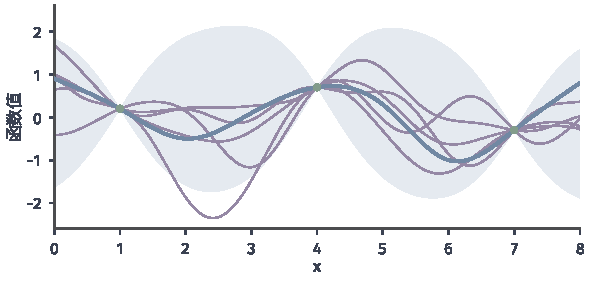
\includegraphics[width=100mm]{figures/05-optimization/05-stochastic-optimization/matplotlib/bo-consistent-functions/figure.pdf}
 \caption{固定的目标与模型的多种可能。粗蓝线是真实目标$f$，绿点是$x=1,4,7$的读数，细紫线是后验分布的五个样本，浅蓝带是后验均值上下各两倍标准差。五条紫线都与读数相符，它们的差异表示认识的不确定，不表示$f$在变化。}
 \label{fig:bo-consistent-functions}
\end{BookInlineFigure}

概率模型是本章区别于前两章的关键。三章都可以只用函数值，分工却在于用这些值做什么，表~\ref{tab:bo-three-methods}作了对比。也要注意，“贝叶斯”这个词不意味着算法每步都在抽签。后面的期望改进给定$\mathcal{D}_t$后完全确定，只有Thompson采样这样的规则才主动使用随机数。

\begin{BookInlineTable}
 \centering
 \caption{三种只用函数值的做法。}
 \label{tab:bo-three-methods}
 \begin{tabular}{lll}
 \toprule
 &用读数做什么&适合的评价预算\\
 \midrule
 零阶随机优化&差分成局部方向&较多，随维数增长\\
 随机搜索&更新搜索状态或分布&较多，候选大量淘汰\\
 贝叶斯优化&建模后计算下次评价的价值&很少，每次都很贵\\
 \bottomrule
 \end{tabular}
\end{BookInlineTable}

\section{概率代理}
\label{sec:bo-surrogate}

怎样用一个读数更新没有被评价的位置的认识？这要求模型做到两件事，一是对每个候选点给出可能函数值的分布，二是说清不同位置之间怎样关联，否则一个位置的读数对其他位置不起作用。满足这两点、用来代替昂贵目标接受查询的模型，称为\term{概率代理}（probabilistic surrogate）。

本节以高斯过程为主说明这个接口。贝叶斯优化并不依赖高斯过程，只要模型能给出相应的预测分布，例如贝叶斯神经网络、树模型的集成，也可以代入后面的选点规则，只是计算的具体公式不同。

\subsection{高斯过程先验}
\label{sec:bo-gp-prior}

先看模型要表达的直觉：相近的参数，通常给出相近的仿真结果。这句话有两层意思。其一，单看一个位置，函数值可能的范围是一个分布。其二，两个位置离得越近，它们的函数值越同涨同落。用协方差描述第二层意思最直接，而最便于计算的联合分布是多元高斯分布。

\begin{definition}[高斯过程]
\label{def:bo-gp}
设$m_0:\bm{C}\to\mathbb{R}$，$k:\bm{C}\times\bm{C}\to\mathbb{R}$。若对任意有限个点$\bm{x}_1,\ldots,\bm{x}_n\in\bm{C}$，向量$(F(\bm{x}_1),\ldots,F(\bm{x}_n))^\top$都服从多元高斯分布，且
\begin{equation}
 \mathbb{E}[F(\bm{x})]=m_0(\bm{x}),\qquad
 \operatorname{Cov}(F(\bm{x}),F(\bm{x}'))=k(\bm{x},\bm{x}'),
 \label{eq:bo-gp}
\end{equation}
就称随机函数$F$是以$m_0$为\term{均值函数}（mean function）、以$k$为\term{协方差核}（covariance kernel）的\term{高斯过程}（Gaussian process，GP）。
\end{definition}

定义只谈有限个点，这正是它好用的地方。一次计算只会碰到有限个位置，手头需要的总是一个普通的多元高斯分布。

核$k$不能随便写。把几个位置的函数值作线性组合，方差必须非负。对任意实数$a_1,\ldots,a_n$，
\[
 0\leq\operatorname{Var}\Bigl(\sum_{i=1}^n a_iF(\bm{x}_i)\Bigr)
 =\sum_{i=1}^n\sum_{j=1}^n a_ia_jk(\bm{x}_i,\bm{x}_j)
 =\bm{a}^\top\bm{K}\bm{a},
\]
其中$\bm{K}$是元素为$k(\bm{x}_i,\bm{x}_j)$的矩阵。所以$k$必须对称，且任意有限组点上的$\bm{K}$都半正定。反过来，满足这两条的$k$配上任意均值函数，确实对应一个高斯过程，证明要用到有限维分布族的相容性与延拓定理，这里只使用结论。

\paragraph{贯穿例的核}
本章取$m_0\equiv0$，并取
\begin{equation}
 k(x,x')=2^{-(x-x')^2}.
 \label{eq:bo-example-kernel}
\end{equation}
它是常用的\term{平方指数核}（squared exponential kernel）$\exp(-(x-x')^2/(2\ell^2))$在$\ell^2=1/(2\ln2)$时的情形，$\ell\approx0.85$。选这个数只是为了手算：间距$1,2,3$的相关系数分别是$1/2,1/16,1/512$。先验方差$k(x,x)=1$表示模型认为函数值大致在$\pm2$内，这与表~\ref{tab:bo-readings}的数量级相符。

取三个相邻位置$x=3,4,5$，核矩阵为
\[
 \bm{K}=\begin{bmatrix}1&1/2&1/16\\1/2&1&1/2\\1/16&1/2&1\end{bmatrix}.
\]
三个顺序主子式依次为
\[
 1,\qquad \frac34,\qquad \frac{135}{256},
\]
全部为正，所以这个$\bm{K}$正定。

\paragraph{核规定了模型愿意相信的变化尺度}
参数$\ell$称为\term{长度尺度}（length scale），它回答“隔多远的两个点就基本无关了”。图~\ref{fig:bo-kernel-scales}比较了三个取值。$\ell$小时相关性衰减快，先验样本频繁起伏；$\ell$大时样本缓慢变化。三条样本用的是同一组随机数，差别完全来自核。

\begin{BookInlineFigure}
 \centering
 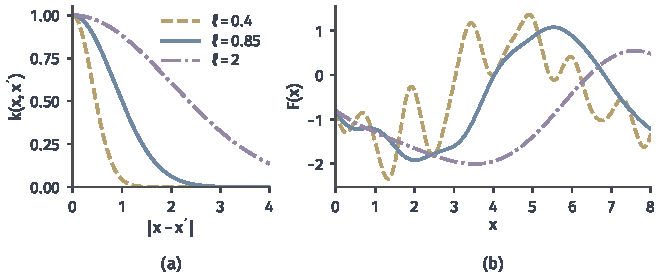
\includegraphics[width=112mm]{figures/05-optimization/05-stochastic-optimization/matplotlib/bo-kernel-scales/figure.pdf}
 \caption{长度尺度的作用。(a)平方指数核随距离的衰减，$\ell=0.85$是贯穿例的取值。(b)用同一组标准正态随机数生成的三条先验样本，线型与(a)对应。长度尺度越大，样本越缓慢。}
 \label{fig:bo-kernel-scales}
\end{BookInlineFigure}

所以核不只是计算工具，它是我们事先下的一个赌注。选了$\ell$，就等于声明目标不会比这个尺度变化得更快。这一声明可能错，第~\ref{sec:bo-model-specification}节专门讨论错了会怎样。

\subsection{后验预测}
\label{sec:bo-posterior}

先用两个位置看清更新是怎么发生的。考虑$x=3$和$x=4$，由式~\eqref{eq:bo-example-kernel}，
\[
 \begin{bmatrix}F(3)\\F(4)\end{bmatrix}
 \sim N\left(\begin{bmatrix}0\\0\end{bmatrix},
 \begin{bmatrix}1&1/2\\1/2&1\end{bmatrix}\right).
\]
现在只评价$x=3$，无噪声地读到$F(3)=1$。关键是把$F(4)$拆成“能由$F(3)$解释的部分”和“剩余部分”：
\[
 F(4)=\tfrac12F(3)+R.
\]

系数$1/2$的选法是让$R$与$F(3)$不相关：
\[
 \operatorname{Cov}(R,F(3))=\tfrac12-\tfrac12\cdot1=0.
\]
联合高斯时不相关就意味着独立，所以读到$F(3)$不改变$R$的分布。$R$的方差为
\[
 \operatorname{Var}(R)=1-2\cdot\tfrac12\cdot\tfrac12+\tfrac14\cdot1=\tfrac34.
\]
代入$F(3)=1$，得到
\[
 F(4)\mid F(3)=1\ \sim\ N\bigl(\tfrac12,\tfrac34\bigr).
\]

虽然没有评价$x=4$，这里的均值从$0$变成了$0.5$，方差从$1$降到了$0.75$。图~\ref{fig:bo-conditional-slice}中，(a)的椭圆是联合分布的等高线，在$F(3)=1$处竖切一刀，得到(b)中的绿线。椭圆是斜的，切线才偏离中心；若相关系数为$0$，椭圆不倾斜，切出来的分布就和先验一样，读数不传递任何信息。

\begin{BookInlineFigure}
 \centering
 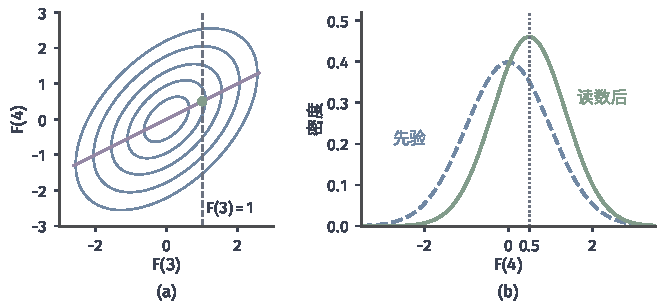
\includegraphics[width=112mm]{figures/05-optimization/05-stochastic-optimization/matplotlib/bo-conditional-slice/figure.pdf}
 \caption{读数怎样传到相关的位置。(a)蓝色椭圆是$(F(3),F(4))$的联合分布等高线，相关系数$1/2$，紫线是条件均值$F(4)=F(3)/2$，竖虚线是读数$F(3)=1$，绿点是该读数下$F(4)$的条件均值。(b)蓝虚线是$F(4)$的先验$N(0,1)$，绿线是读数后的$N(1/2,3/4)$。}
 \label{fig:bo-conditional-slice}
\end{BookInlineFigure}

一般情形只是把这种拆分写成矩阵。记$\bm{K}_t$为$t\times t$矩阵，元素是$k(\bm{x}_i,\bm{x}_j)$；$\bm{k}_t(\bm{x})$是长度$t$的向量，第$i$个分量是$k(\bm{x},\bm{x}_i)$；$\bm{y}_t$是读数向量；$\bm{m}_{0,t}$是先验均值在各评价点处的取值。读数可能含噪，设$y_i=F(\bm{x}_i)+\varepsilon_i$，$\varepsilon_i\sim N(0,\tau^2)$，彼此独立，且与$F$独立；$\tau=0$表示无噪声。

\begin{theorem}[高斯过程的后验]
\label{thm:bo-posterior}
设$F$是高斯过程，评价点固定，核与噪声参数已知，$\bm{A}_t=\bm{K}_t+\tau^2\bm{I}$可逆。则给定$\bm{y}_t$，$F$仍是高斯过程，其后验均值与后验协方差为
\begin{align}
 m_t(\bm{x})&=m_0(\bm{x})+\bm{k}_t(\bm{x})^\top\bm{A}_t^{-1}(\bm{y}_t-\bm{m}_{0,t}),
 \label{eq:bo-post-mean}\\
 c_t(\bm{x},\bm{x}')&=k(\bm{x},\bm{x}')-\bm{k}_t(\bm{x})^\top\bm{A}_t^{-1}\bm{k}_t(\bm{x}').
 \label{eq:bo-post-cov}
\end{align}
特别地，记$s_t^2(\bm{x})=c_t(\bm{x},\bm{x})$，则
\begin{equation}
 F(\bm{x})\mid\mathcal{D}_t\sim N\bigl(m_t(\bm{x}),s_t^2(\bm{x})\bigr).
 \label{eq:bo-post-marginal}
\end{equation}
\end{theorem}

\begin{proof}
取任意有限组候选点，$F$在这些点与读数向量合起来是联合高斯的。对一个候选点$\bm{x}$，令
\[
 \bm{a}=\bm{A}_t^{-1}\bm{k}_t(\bm{x}).
\]
定义剩余量
\[
 R(\bm{x})=F(\bm{x})-m_0(\bm{x})-\bm{a}^\top(\bm{y}_t-\bm{m}_{0,t}),
\]
这里$\bm{y}_t$理解为随机向量。

读数的协方差矩阵是$\bm{A}_t$，$F(\bm{x})$与读数的协方差向量是$\bm{k}_t(\bm{x})$，于是
\[
 \operatorname{Cov}(R(\bm{x}),\bm{y}_t)=\bm{k}_t(\bm{x})-\bm{A}_t\bm{a}=\bm{0}.
\]
联合高斯下，不相关推出独立，所以$\mathcal{D}_t$不改变$R(\bm{x})$的分布，它的均值仍是$0$。把读数的实际值代入$F(\bm{x})$的分解式，条件均值就是式~\eqref{eq:bo-post-mean}。

设$R'$是$\bm{x}'$处对应的剩余量，$\bm{a}'=\bm{A}_t^{-1}\bm{k}_t(\bm{x}')$。给定读数后$F(\bm{x})$与$F(\bm{x}')$的随机部分只有$R$与$R'$，因此
\[
 \begin{aligned}
 \operatorname{Cov}(R,R')
 &=k(\bm{x},\bm{x}')-\bm{a}^\top\bm{k}_t(\bm{x}')-\bm{a}'^\top\bm{k}_t(\bm{x})+\bm{a}^\top\bm{A}_t\bm{a}'\\
 &=k(\bm{x},\bm{x}')-\bm{k}_t(\bm{x})^\top\bm{A}_t^{-1}\bm{k}_t(\bm{x}').
 \end{aligned}
\]
这就是式~\eqref{eq:bo-post-cov}。任意有限组点上同样成立，所以后验仍是高斯过程。
\end{proof}

这个证明用到联合高斯下不相关推出独立，条件高斯的一般公式及其矩阵推导可参考\BookChapterRef{chap:random-vectors}{卷七第6章“随机向量”}；把核视为函数上的先验来做回归的一般理论，可参考\BookChapterRef{chap:nonparametric-inference}{卷八第2章“非参数分布与函数推断”}。

读这两个公式时，注意三件事。第一，后验方差~\eqref{eq:bo-post-cov}不含读数$\bm{y}_t$，只取决于评价放在哪里，好读数和坏读数减少的不确定性相同。第二，无噪声时$m_t(\bm{x}_i)=y_i$，$s_t(\bm{x}_i)=0$，模型穿过读数。第三，$c_t(\bm{x},\bm{x}')$要保留，不能只留方差，后面联合抽样和批量选点都要用到不同候选点之间的后验协方差。

定理假设评价点固定，而实际的$\bm{x}_{t+1}$依赖之前的读数。公式仍然成立，原因是选点规则只看$\mathcal{D}_t$：写出整条数据的似然时，选点这一步给出的因子不依赖$F$，它在归一化时被消去，后验仍只由读数的高斯因子决定。条件分布的一般含义可参考\BookChapterRef{chap:conditional-expectation}{卷七第10章“条件期望”}。

\paragraph{贯穿例：三个读数后的后验}
评价$x=1,4,7$，读数$\bm{y}_3=(0.2,0.7,-0.3)^\top$。核矩阵是
\[
 \bm{K}_3=\begin{bmatrix}1&2^{-9}&2^{-36}\\2^{-9}&1&2^{-9}\\2^{-36}&2^{-9}&1\end{bmatrix},
\]
其中$2^{-9}\approx0.002$。解线性方程$\bm{K}_3\bm{w}=\bm{y}_3$，得到
\[
 \bm{w}=\bm{K}_3^{-1}\bm{y}_3\approx(0.1986,\ 0.7002,\ -0.3014)^\top.
\]

看未评价的$x=6$。到三个评价点的距离是$5,2,1$，所以
\[
 \bm{k}_3(6)=(2^{-25},\ 1/16,\ 1/2)^\top.
\]
由式~\eqref{eq:bo-post-mean}，
\[
 m_3(6)=\bm{k}_3(6)^\top\bm{w}\approx0.0625\times0.7002-0.5\times0.3014\approx-0.107.
\]
由式~\eqref{eq:bo-post-cov}，
\[
 s_3^2(6)=1-\bm{k}_3(6)^\top\bm{K}_3^{-1}\bm{k}_3(6)\approx0.746,
\]
即$s_3(6)\approx0.864$。把$2^{-9}$按$0$手算，会得到$-0.106$和$0.746$，差别只在第三位小数。

图~\ref{fig:bo-posterior-sequence}是读数逐个加入时的后验。第一个读数只影响$x=1$附近，其他地方后验几乎还是先验。后面的读数逐段收紧不确定带。深色的后验均值并没有“找到”$x=6$的谷，这很自然：三个点都不在谷里，模型没有理由想象到它。正是这种“均值还不低、但不确定带向下伸得很远”的区域，需要由下一节的规则来评估。

\begin{BookInlineFigure}
 \centering
 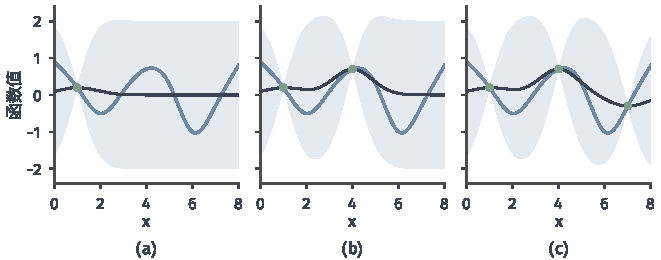
\includegraphics[width=112mm]{figures/05-optimization/05-stochastic-optimization/matplotlib/bo-posterior-sequence/figure.pdf}
 \caption{后验随读数更新。蓝线是目标$f$，深色线是后验均值$m_t$，浅蓝带是$m_t\pm2s_t$，绿点是读数。(a)只有$x=1$；(b)加入$x=4$；(c)加入$x=7$。}
 \label{fig:bo-posterior-sequence}
\end{BookInlineFigure}

计算量也要记一笔。对$\bm{A}_t$作一次Cholesky分解约需$t^3/3$次运算，见\BookChapterRef{chap:direct-linear-solvers}{卷二第12章“线性方程的直接求解”}；此后每个候选点的均值需$O(t)$次运算，方差需$O(t^2)$次。贝叶斯优化中$t$通常只有几十到几百，这笔开销相对一次昂贵评价可以忽略，第~\ref{sec:bo-budget}节再核算它什么时候不能忽略。

\subsection{模型设定}
\label{sec:bo-model-specification}

上面都假定核与噪声参数已知。实际问题中$\ell$、先验方差等\term{超参数}（hyperparameter）并不知道，这就有了本节的问题：模型的这些设定错了会怎样，又该如何对待它们的不确定性。

\paragraph{边缘似然与直接代入}
常用办法是看哪组超参数最能解释已有读数。把超参数记为$\bm{\theta}$，读数的边缘分布是$N(\bm{m}_{0,t},\bm{A}_t(\bm{\theta}))$，其对数密度
\begin{equation}
 \log p(\bm{y}_t\mid\bm{\theta})=-\tfrac12\bm{r}^\top\bm{A}_t^{-1}\bm{r}-\tfrac12\log\det\bm{A}_t-\tfrac t2\log(2\pi)
 \label{eq:bo-marginal-likelihood}
\end{equation}
称为\term{边缘似然}（marginal likelihood）的对数，其中$\bm{r}=\bm{y}_t-\bm{m}_{0,t}$。第一项奖励拟合读数，第二项惩罚过于灵活的模型。常见做法是取使它最大的$\widehat{\bm{\theta}}$，然后把它当作真值代入定理~\ref{thm:bo-posterior}。

直接代入回避了一个事实：超参数本身也拿不准。把不确定性计入的做法是对超参数的后验分布积分，得到混合预测。若$\bm{\theta}$只有有限个候选，后验概率为$w_j$，候选$j$给出的均值和方差为$m^{(j)},v^{(j)}$，则由全方差公式，
\begin{equation}
 \begin{gathered}
 \bar m=\sum_jw_jm^{(j)},\\
 \bar v=\sum_jw_jv^{(j)}+\sum_jw_j\bigl(m^{(j)}-\bar m\bigr)^2.
 \end{gathered}
 \label{eq:bo-mixture}
\end{equation}
第一项是平均的方差，第二项是不同超参数之间的分歧。第二项非负，所以混合预测的方差不小于各候选方差的加权平均，分歧越大增加越多。

\paragraph{例：两个候选长度尺度}
仍用三个读数，比较$\ell\approx0.85$和$\ell=3$，两者的先验概率相等。由式~\eqref{eq:bo-marginal-likelihood}算得对数边缘似然分别约为$-3.067$和$-3.106$，几乎相同，按贝叶斯公式得到后验概率
\[
 w_1\approx0.51,\qquad w_2\approx0.49.
\]
三个读数不足以区分这两种解释。

两种解释在$x=6$处的预测却差得很远：
\[
 \begin{aligned}
 \ell\approx0.85:&\quad m=-0.107,\quad v=0.746,\\
 \ell=3:&\quad m=0.093,\quad v=0.015.
 \end{aligned}
\]
由式~\eqref{eq:bo-mixture}，混合预测的均值和方差为
\[
 \bar m\approx-0.009,\qquad \bar v\approx0.398.
\]

若只取$\ell=3$直接代入，方差$0.015$比混合预测小了约$26$倍。图~\ref{fig:bo-model-specification}(b)显示，长度尺度大的模型在$x=6$处把标准差算得很小，而真实值$-1.0$远在它的不确定带之外。这正是直接代入的风险：边缘似然选中了一个看上去同样好的解释，却丢掉了“还有另一种解释”这条信息。

\begin{BookInlineFigure}
 \centering
 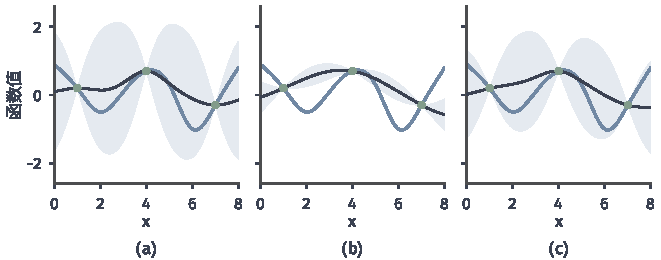
\includegraphics[width=112mm]{figures/05-optimization/05-stochastic-optimization/matplotlib/bo-model-specification/figure.pdf}
 \caption{同样三个读数下的不同模型设定。蓝线是目标，深色线是预测均值，浅蓝带是均值上下两倍标准差。(a)$\ell\approx0.85$；(b)$\ell=3$，不确定带很窄，却没有盖住$x=6$附近的谷；(c)两者按边缘似然加权的混合预测，读数之间的方差反映了两种解释的分歧。}
 \label{fig:bo-model-specification}
\end{BookInlineFigure}

\paragraph{设定要回到问题来检查}
长度尺度隐含一个假设：同样的距离代表同样的变化幅度。输入的尺度是否合适直接关系这个假设。例如学习率类的参数从$10^{-4}$变到$1$，在原始坐标上$10^{-4}$与$10^{-3}$几乎重合，但它们的效果可能相差很多；改用$\log_{10}$坐标后，相邻量级的距离才都等于$1$。多维问题中各坐标的单位不同，通常给每个坐标各设一个长度尺度。

先验的光滑程度也要与问题相符。平方指数核的样本无穷次可微，目标若有折点或跳跃，模型会用过短的长度尺度去迁就，导致全局方差偏大。可微性有限的核，如Mat\'ern族，常用来表达较弱的光滑假设。

读数本身可以检验模型。依次去掉第$i$个读数，用其余读数预测它，得到留一标准化残差
\begin{equation}
 e_i=\frac{y_i-m_{-i}(\bm{x}_i)}{\sqrt{s_{-i}^2(\bm{x}_i)+\tau^2}}.
 \label{eq:bo-loo}
\end{equation}
模型合适时这些数大致像标准正态的取值，大量绝对值超过$3$说明模型与读数不符。贯穿例的三个读数相距较远，其余读数几乎不影响被去掉的位置，$e_i$约等于读数本身，$0.2,0.7,-0.3$都不大。可是读数太少时这个检查的力量也很弱，通过检查不等于模型正确。

低方差只说明“在这个模型下”不确定性小，不能直接等同于目标已经被准确掌握。图~\ref{fig:bo-model-specification}(b)是一个具体的反例。后面几节的后验都默认超参数固定，这是为了把选点逻辑讲清楚；实际使用时，每轮通常重新估计或积分超参数，第~\ref{sec:bo-noise-variances}节还会看到这样做对方差的影响。

\section{采集函数}
\label{sec:bo-acquisition}

后验告诉了我们每个候选点上函数值的分布，但它没有说下一次该评价哪里。接下来要弄清：怎样把后验转成一个可以比较大小的分数？这个分数称为\term{采集函数}（acquisition function），记作$\alpha_t(\bm{x})$，下一个评价点取使它最大的位置。

好的分数要处理一对矛盾。后验均值低的地方看起来有希望，这是\emph{利用}；后验方差大的地方我们知之甚少，那里可能藏着好东西，这是\emph{探索}。各种采集函数的差别就在于用什么方式把两者结合起来。

本节先假定观测无噪声，当前已观测的最好值就是
\begin{equation}
 b_t=\min_{i\leq t}f(\bm{x}_i).
 \label{eq:bo-incumbent}
\end{equation}
下面统一按最小化比较。例子都用$t=3$时贯穿例的后验，$b_3=-0.3$，取整数候选点。

\subsection{改进概率（PI）}
\label{sec:bo-pi}

最朴素的想法是问：在这个位置评价，有多大可能比现在最好的结果更好？再要求至少好出一个幅度$\xi\geq0$，得到\term{改进概率}（probability of improvement，PI）：
\begin{equation}
 \mathrm{PI}_t(\bm{x})=\mathbb{P}\bigl(F(\bm{x})<b_t-\xi\mid\mathcal{D}_t\bigr)
 =\Phi\left(\frac{b_t-\xi-m_t(\bm{x})}{s_t(\bm{x})}\right),
 \label{eq:bo-pi}
\end{equation}
其中$s_t(\bm{x})>0$，$\Phi$是标准正态分布函数。$s_t(\bm{x})=0$时，函数值已确定，$\mathrm{PI}$依$m_t(\bm{x})<b_t-\xi$是否成立取$1$或$0$。

PI只数“是否过线”，不问过线之后好多少。比较两个候选，取$b_t=0$，$\xi=0$，
\[
 \text{A}:\ F\sim N(-0.1,\ 0.1^2),\qquad
 \text{B}:\ F\sim N(0.5,\ 1).
\]
代入式~\eqref{eq:bo-pi}，
\[
 \mathrm{PI}(\text{A})=\Phi(1)\approx0.841,\qquad
 \mathrm{PI}(\text{B})=\Phi(-0.5)\approx0.309.
\]
PI选A。图~\ref{fig:bo-pi-vs-ei}的绿色面积就是这两个概率。可是A即使成功也只改善零点几，B虽不常成功，一旦成功可能改善很多。

\begin{BookInlineFigure}
 \centering
 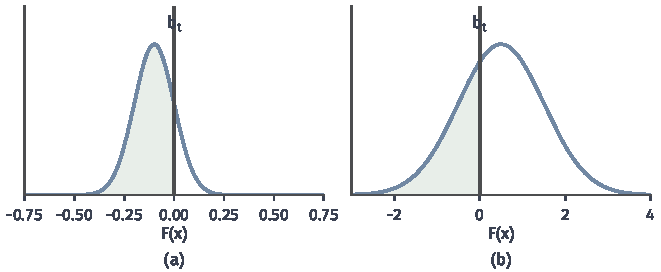
\includegraphics[width=112mm]{figures/05-optimization/05-stochastic-optimization/matplotlib/bo-pi-vs-ei/figure.pdf}
 \caption{改进的概率与幅度。蓝线是候选点函数值的后验密度，深灰竖线是当前最好值$b_t=0$，浅绿面积是改进概率。(a)候选A：$N(-0.1,0.1^2)$，大概率过线，但过线幅度很小。(b)候选B：$N(0.5,1)$，概率较小，但左尾可以伸得很远。两图横轴比例不同。}
 \label{fig:bo-pi-vs-ei}
\end{BookInlineFigure}

$\xi$的作用可以这样看。$\xi=0$时，紧贴着当前最好点的位置，后验均值几乎等于$b_t$，方差几乎为零，PI接近$1/2$，后面的图中可以看到，PI的最大点恰好贴在已观测的最好点旁边，这样的评价几乎不提供新信息。取$\xi>0$把门槛压低，这种贴边的小改进就不算数了。可是$\xi$取多大没有普适答案，它取决于函数值的尺度。

\subsection{期望改进（EI）}
\label{sec:bo-ei}

PI的缺陷指明了修改方向：把幅度也算进去。若在$\bm{x}$评价，新的最好值相比$b_t$的改善量是
\[
 \bigl(b_t-F(\bm{x})\bigr)_+=\max\{b_t-F(\bm{x}),0\}.
\]
没有改善时计为$0$，因为最好值不会变差。这个改善量的后验期望称为\term{期望改进}（expected improvement，EI）：
\begin{equation}
 \mathrm{EI}_t(\bm{x})=\mathbb{E}\bigl[(b_t-F(\bm{x}))_+\mid\mathcal{D}_t\bigr].
 \label{eq:bo-ei-def}
\end{equation}

\begin{theorem}[期望改进的闭式]
\label{thm:bo-ei}
设$F(\bm{x})\mid\mathcal{D}_t\sim N(m,s^2)$。若$s>0$，记$z=(b_t-m)/s$，则
\begin{equation}
 \mathrm{EI}_t(\bm{x})=(b_t-m)\Phi(z)+s\phi(z),
 \label{eq:bo-ei}
\end{equation}
其中$\Phi$、$\phi$分别是标准正态分布函数和密度函数。若$s=0$，则
\begin{equation}
 \mathrm{EI}_t(\bm{x})=(b_t-m)_+.
 \label{eq:bo-ei-zero}
\end{equation}
\end{theorem}

\begin{proof}
$s=0$时$F(\bm{x})=m$是确定的数，改善量就是$(b_t-m)_+$。

设$s>0$，把$F(\bm{x})$写成$m+sW$，$W\sim N(0,1)$，则
\[
 b_t-F(\bm{x})=s(z-W).
\]
所以
\[
 \mathrm{EI}_t(\bm{x})=s\int_{-\infty}^{z}(z-w)\phi(w)\,\mathrm{d}w
 =sz\Phi(z)-s\int_{-\infty}^{z}w\phi(w)\,\mathrm{d}w.
\]

由$\phi'(w)=-w\phi(w)$，后一个积分等于$-\phi(z)$，于是
\[
 \mathrm{EI}_t(\bm{x})=s\bigl(z\Phi(z)+\phi(z)\bigr).
\]
再用$sz=b_t-m$，即得式~\eqref{eq:bo-ei}。
\end{proof}

式~\eqref{eq:bo-ei}的两项正好对应利用和探索。第一项是均值带来的改进，乘上改进发生的概率；第二项随不确定性$s$增大。两者的取舍可以用导数说得更准确。把$\mathrm{EI}$看成$(m,s)$的函数，并用$\phi'(z)=-z\phi(z)$，得到
\begin{equation}
 \frac{\partial\mathrm{EI}}{\partial m}=-\Phi(z)<0,\qquad
 \frac{\partial\mathrm{EI}}{\partial s}=\phi(z)>0.
 \label{eq:bo-ei-derivatives}
\end{equation}
均值越低EI越大，方差越大EI也越大，$s>0$时总如此。$s$的增大不是白来的奖励：只有左尾越过$b_t$的部分才计入期望，右尾再长也不扣分。

回到候选A、B，$b_t=0$。代入式~\eqref{eq:bo-ei}：
\[
 \mathrm{EI}(\text{A})=0.1\,\Phi(1)+0.1\,\phi(1)\approx0.108,
\]
\[
 \mathrm{EI}(\text{B})=-0.5\,\Phi(-0.5)+\phi(0.5)\approx0.198.
\]
EI选B，把PI的结论翻转了。

\paragraph{贯穿例}
看$t=3$时的$x=6$和$x=8$。由第~\ref{sec:bo-posterior}节的后验，
\[
 m_3(6)=-0.107,\quad s_3(6)=0.864,\qquad
 m_3(8)=-0.151,\quad s_3(8)=0.866.
\]
对$x=8$计算标准化量
\[
 z=\frac{-0.3+0.151}{0.866}\approx-0.172,
\]
查表得$\Phi(z)\approx0.432$，$\phi(z)\approx0.393$，于是
\[
 \mathrm{EI}_3(8)\approx-0.149\times0.432+0.866\times0.393\approx0.276.
\]
同样算得$\mathrm{EI}_3(6)\approx0.257$。两者很接近，$x=8$略高，原因是$x=6$距离高读数$0.7$的$x=4$只有$2$，$x=8$则距离更远。

\subsection{置信下界（LCB）}
\label{sec:bo-lcb}

第三种想法不计算期望，而是持乐观态度：把每个位置都按它“可能的好情形”来看，选最好的那个。\term{置信下界}（lower confidence bound，LCB）规则选择使
\begin{equation}
 \mathrm{LCB}_t(\bm{x})=m_t(\bm{x})-\kappa_ts_t(\bm{x})
 \label{eq:bo-lcb}
\end{equation}
最小的位置，其中$\kappa_t\geq0$控制探索程度。它是最大化问题中GP-UCB规则的最小化对应形式。$\kappa_t=0$时只看均值，$\kappa_t$越大越偏向未知区域。

规则本身很简单，容易误读的是名字。取$\kappa=1.96$时，$m_t-1.96s_t$是单个固定点的$95\%$可信下限，但用它选点时，它并不自动成为有效的置信界。原因有两个。其一，选点时同时比较了所有候选，就算只有$9$个相互独立的候选，全部覆盖的概率也只有
\[
 0.95^9\approx0.63.
\]
其二，$\bm{x}_{t+1}$是看过数据之后才选出来的，它不是一个事先固定的点。要称为有效置信界，必须说明模型、噪声以及$\kappa_t$随时间的取值，第~\ref{sec:bo-guarantees}节给出一组这样的条件。在那之前，$\kappa_t$只应理解为一个探索权重。

\paragraph{三种规则的比较}
表~\ref{tab:bo-acq-values}把贯穿例整数候选上的结果放在一起。三种规则在这一步都选$x=8$，但它们在其他候选上的分数高低并不相同：$\mathrm{LCB}$在几乎未知的位置差别很小，EI和PI则能根据均值差别作区分。

\begin{BookInlineTable}
 \centering
 \caption{贯穿例$t=3$时整数候选上的后验与采集分数，$b_3=-0.3$，PI取$\xi=0$，LCB取$\kappa=2$。已观测位置$x=1,4,7$上标准差为$0$。粗体是各列选中的候选。}
 \label{tab:bo-acq-values}
 \begin{tabular}{cccccc}
 \toprule
 $x$&$m_3$&$s_3$&PI&EI&LCB\\
 \midrule
 0&0.099&0.866&0.322&0.182&$-1.633$\\
 1&0.200&0&0&0&0.200\\
 2&0.143&0.864&0.304&0.167&$-1.585$\\
 3&0.363&0.864&0.222&0.110&$-1.365$\\
 4&0.700&0&0&0&0.700\\
 5&0.331&0.864&0.233&0.117&$-1.396$\\
 6&$-0.107$&0.864&0.412&0.257&$-1.835$\\
 7&$-0.300$&0&0&0&$-0.300$\\
 8&$-0.151$&0.866&$\mathbf{0.432}$&$\mathbf{0.276}$&$\mathbf{-1.883}$\\
 \bottomrule
 \end{tabular}
\end{BookInlineTable}

图~\ref{fig:bo-acq-compare}画出了各规则在连续的$x$上的分数。第二行的黄线中，$\xi=0$的PI在$x=7$两侧紧贴读数处接近$1/2$，它的连续最大点就在$x=7$旁边，这就是前面说的贴边现象；$x=7$这一点本身函数值已知，不可能再改进，PI为$0$，曲线在此处断开。取$\xi=0.3$后，这个峰消失。第三行的EI在已观测点为$0$，在两块不确定区域形成山峰，最大点在$x=8$。第四行的LCB随$\kappa$增大，最小点从$x=8$移向更靠中间的未知区域，$\kappa=3$时连续最小点在$x\approx5.68$。

\begin{BookInlineFigure}
 \centering
 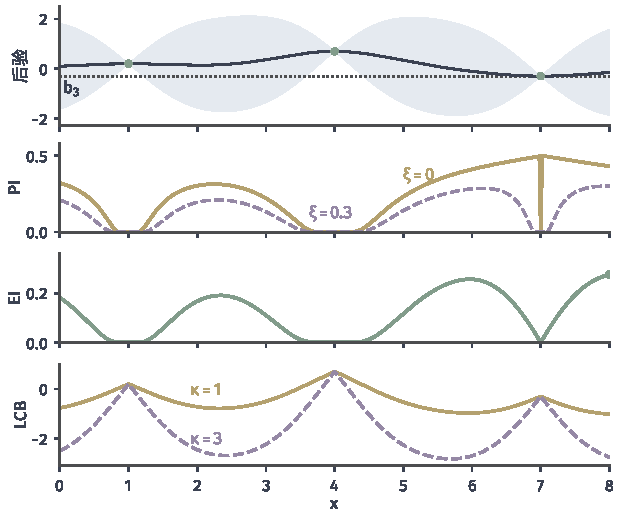
\includegraphics[width=105mm]{figures/05-optimization/05-stochastic-optimization/matplotlib/bo-acq-compare/figure.pdf}
 \caption{三种采集函数的比较，$t=3$，读数在$x=1,4,7$。第一行：深色线是后验均值，浅蓝带是均值上下两倍标准差，点线是$b_3$。第二行：改进概率，黄线$\xi=0$，紫虚线$\xi=0.3$。第三行：期望改进，绿点是最大点。第四行：置信下界，黄线$\kappa=1$，紫虚线$\kappa=3$，选点取最小点。}
 \label{fig:bo-acq-compare}
\end{BookInlineFigure}

\subsection{Thompson 采样}
\label{sec:bo-thompson}

前三种规则都把后验压缩成一个分数。\term{Thompson采样}（Thompson sampling）换了一种做法：不算分数，从当前后验抽取一整条函数$\widetilde{F}$，假装它就是真实目标，然后选它的最小点：
\begin{equation}
 \bm{x}_{t+1}\in\argmin_{\bm{x}\in\bm{C}}\widetilde{F}(\bm{x}),\qquad
 \widetilde{F}\sim F\mid\mathcal{D}_t.
 \label{eq:bo-thompson}
\end{equation}
一个位置被选中的概率，等于后验认为它是最小点的概率。乐观与谨慎不需要权重来调，而由后验分布本身决定：不确定的地方抽样起伏大，有机会被选中，但机会并不独占。

\paragraph{抽样要联合}
在有限候选集$\bm{x}_{1}',\ldots,\bm{x}_{N}'$上，抽样要从多元高斯分布$N(\bm{\mu},\bm{\Sigma})$抽取，$\bm{\mu}$和$\bm{\Sigma}$分别是后验均值向量和后验协方差矩阵。常用办法是作Cholesky分解$\bm{\Sigma}=\bm{L}\bm{L}^\top$，抽取标准正态向量$\bm{z}$，令
\begin{equation}
 \widetilde{\bm{F}}=\bm{\mu}+\bm{L}\bm{z}.
 \label{eq:bo-joint-sample}
\end{equation}

以$t=3$时的候选$x=6,8$为例。后验协方差矩阵和分解为
\[
 \bm{\Sigma}=\begin{bmatrix}0.746&-0.187\\-0.187&0.750\end{bmatrix},\qquad
 \bm{L}=\begin{bmatrix}0.864&0\\-0.217&0.838\end{bmatrix}.
\]
这里协方差是负的，这有一点反直觉：两点都与$x=7$相关，而$F(7)$已经确定，第~\ref{sec:bo-sequential}节会解释这个负号。

取$\bm{z}=(1,-0.5)^\top$，代入式~\eqref{eq:bo-joint-sample}，
\[
 \widetilde{F}(6)=-0.107+0.864=0.757,\quad
 \widetilde{F}(8)=-0.151-0.217-0.419=-0.787,
\]
这条样本的最小点在$x=8$。取$\bm{z}=(-1,0.5)^\top$，则
\[
 \widetilde{F}(6)=-0.971,\quad\widetilde{F}(8)=0.485,
\]
这条样本选$x=6$。两种结果都可能发生，选点因此带有随机性。

若把各点的边际分布独立抽样，得到的就不是后验函数。图~\ref{fig:bo-ts-paths}对比了在$0.1$网格上的两种抽样。(a)联合抽样是一条光滑曲线，穿过全部读数。(b)独立抽样忽略了相邻点的相关性，成了一串噪声，最小点总会落在方差最大的某处，这不是后验认为最可能的最小点。按20000条联合样本统计，最小点约四分之一的机会落在$x=8$附近，约四分之一的机会落在$x=6$附近，其余分散到$x=0$和$x=2$等位置。

\begin{BookInlineFigure}
 \centering
 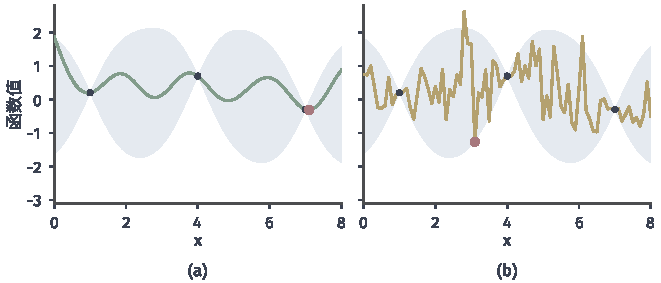
\includegraphics[width=112mm]{figures/05-optimization/05-stochastic-optimization/matplotlib/bo-ts-paths/figure.pdf}
 \caption{联合抽样与边际独立抽样。浅蓝带是$t=3$的后验均值上下两倍标准差，黑点是读数，红点是样本的最小点。(a)联合抽样得到的绿色曲线是一条可能的函数。(b)各网格点独立抽样得到的黄线不对应任何一条函数，把它的最小点当作选点并无依据。}
 \label{fig:bo-ts-paths}
\end{BookInlineFigure}

计算上，$N$个候选的联合抽样要作一次$O(N^3)$的分解。连续搜索域上不能抽取真正的无穷维函数，通常在较大的候选集上离散化，或用有限维随机特征近似，这些都是近似的来源。

\subsection{知识梯度（补充）}
\label{sec:bo-kg}

EI衡量的是“这次读数本身比现在最好的值低多少”。可是我们最终要交付的是推荐解，而一次读数即使本身不好，也可能让我们更清楚哪个位置该推荐。本小节换一个问题：这次观测能让最终推荐改善多少？

\paragraph{定义}
取一个推荐集合$\bm{R}\subseteq\bm{C}$，当前的最优推荐价值是后验均值的最小值$\min_{\bm{x}'\in\bm{R}}m_t(\bm{x}')$。设想在$\bm{x}$再观测一次，更新后的后验均值为$m_{t+1}$，它依赖尚未发生的读数，因而是随机的。\term{知识梯度}（knowledge gradient，KG）定义为
\begin{equation}
 \mathrm{KG}_t(\bm{x})=\min_{\bm{x}'\in\bm{R}}m_t(\bm{x}')-\mathbb{E}\Bigl[\min_{\bm{x}'\in\bm{R}}m_{t+1}(\bm{x}')\,\Bigm|\,\mathcal{D}_t,\bm{x}_{t+1}=\bm{x}\Bigr].
 \label{eq:bo-kg}
\end{equation}
更新后的均值以当前均值为期望，也就是
\[
 \mathbb{E}\bigl[m_{t+1}(\bm{x}')\mid\mathcal{D}_t\bigr]=m_t(\bm{x}').
\]
$\min$是凹函数，凹函数的期望不超过期望处的函数值（Jensen不等式），所以$\mathrm{KG}_t(\bm{x})\geq0$。

下一次读数的预测分布是$N(m_t(\bm{x}),s_t^2(\bm{x})+\tau^2)$，把标准化的预测残差记作$Z\sim N(0,1)$。把定理~\ref{thm:bo-posterior}应用于“以当前后验为先验、只含这一个观测”的情形，可得
\begin{equation}
 m_{t+1}(\bm{x}')=m_t(\bm{x}')+\widetilde{\sigma}_t(\bm{x}',\bm{x})Z,\quad
 \widetilde{\sigma}_t(\bm{x}',\bm{x})=\frac{c_t(\bm{x}',\bm{x})}{\sqrt{s_t^2(\bm{x})+\tau^2}}.
 \label{eq:bo-kg-update}
\end{equation}
每个推荐点的后验均值都随同一个$Z$线性移动，斜率取决于它与被观测位置的后验协方差。式~\eqref{eq:bo-kg}中的期望因此是一维积分，有限的$\bm{R}$上可以用分段线性包络精确算出，也可以用数值积分。

\paragraph{例：观测一个不推荐的位置}
取$\bm{R}=\{6,7\}$，当前后验均值$m_3(6)=-0.107$，$m_3(7)=-0.3$，当前最优推荐是$x=7$，价值$-0.3$。考虑观测$x=5$，它本身不在$\bm{R}$里。$x=7$已观测，$c_3(7,5)=0$，均值不动。由$c_3(6,5)\approx0.438$和$s_3(5)\approx0.864$，
\[
 \widetilde{\sigma}_3(6,5)\approx\frac{0.438}{0.864}\approx0.507.
\]

新的最优推荐价值是$\min\{-0.3,\ -0.107+0.507Z\}$。这个最小值可以写成$-0.3$减去$-0.3$与第二项之差的正部，代入式~\eqref{eq:bo-kg}，$\mathrm{KG}$恰好是阈值为$-0.3$的EI公式，只是均值和标准差换成$-0.107$与$0.507$：
\[
 \mathrm{KG}_3(5)\approx(-0.193)\Phi(-0.381)+0.507\,\phi(-0.381)\approx0.120.
\]
这个$x=5$的读数本身比$-0.3$低的可能性不大，因而$\mathrm{EI}_3(5)\approx0.117$，它的价值主要来自让我们更好地判断$x=6$。此处的KG同样不要求评价点属于$\bm{R}$，这是它与EI的不同，也允许最后推荐一个未曾评价的位置。

图~\ref{fig:bo-kg-vs-ei}比较了EI和取$\bm{R}$为$0.1$网格时的KG。两者的形状相近，但KG的最大点在$x\approx7.1$，紧靠当前最好点。在无噪声且核很光滑的模型中，贴着已知点再读一次，相当于测得该处的斜率，它能改变整段后验均值的最小位置，所以KG偏爱这里；而在恰好已观测的点上，读数不带来任何新信息，KG降为$0$，图中出现几个尖口。

\begin{BookInlineFigure}
 \centering
 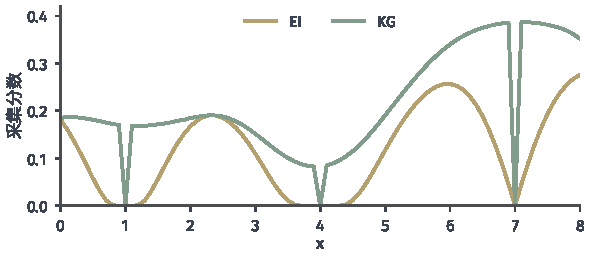
\includegraphics[width=100mm]{figures/05-optimization/05-stochastic-optimization/matplotlib/bo-kg-vs-ei/figure.pdf}
 \caption{EI与KG的对比，$t=3$，无噪声观测。黄线是期望改进，绿线是知识梯度（推荐集合为$0.1$网格，期望由$401$个等分位点数值积分）。KG在已观测点$x=1,4,7$上为$0$，在紧邻这些点的位置却不为$0$。}
 \label{fig:bo-kg-vs-ei}
\end{BookInlineFigure}

KG的计算比EI贵，并且对模型更敏感。一般的实验设计问题以信息价值安排观测，可参考\BookChapterRef{chap:observation-experiment-design}{卷八第9章“观测与实验设计”}；本章只把KG作为一种选点规则，在第~\ref{sec:bo-noisy}节有噪声时会再次用到它。

\section{顺序求解}
\label{sec:bo-sequential}

有了代理和采集函数，本节把它们接成一个完整的循环，回答一个具体问题：在预算$T$内，每一轮应当按什么次序做哪些计算，新读数又怎样改变下一轮的决策。

\paragraph{主要思想}
循环由两层组成，见图~\ref{fig:bo-loop}。外层是昂贵的真实评价，内层是便宜的计算：用数据建模，把模型转成分数，求分数的最大点。如果外层一次要几小时，内层花几秒钟算一个好的选点就很划算。

\begin{BookInlineFigure}
 \centering
 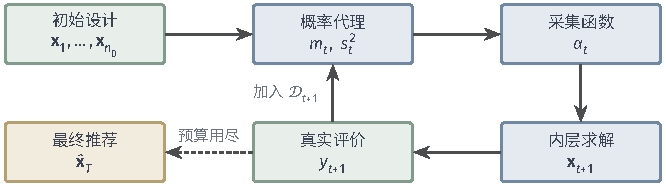
\includegraphics[width=112mm]{figures/05-optimization/05-stochastic-optimization/tikz/bo-loop/figure.pdf}
 \caption{贝叶斯优化的循环。绿框是需要运行真实目标的步骤，蓝框是只涉及代理模型的便宜计算，黄框是最后的输出。每轮读数加入$\mathcal{D}_{t+1}$，再回到概率代理更新。}
 \label{fig:bo-loop}
\end{BookInlineFigure}

每轮不必从头重算。第~\ref{sec:bo-posterior}节的后验本身是一个高斯过程，下一个读数相对它只是\emph{一个}新观测，把定理~\ref{thm:bo-posterior}应用于“以$(m_t,c_t)$为先验、只含一个观测”的情形，就得到更新式。记$\bm{x}^+=\bm{x}_{t+1}$，$y^+=y_{t+1}$，$v=s_t^2(\bm{x}^+)+\tau^2$，则
\begin{align}
 m_{t+1}(\bm{x})&=m_t(\bm{x})+\frac{c_t(\bm{x},\bm{x}^+)}{v}\bigl(y^+-m_t(\bm{x}^+)\bigr),
 \label{eq:bo-update-mean}\\
 c_{t+1}(\bm{x},\bm{x}')&=c_t(\bm{x},\bm{x}')-\frac{c_t(\bm{x},\bm{x}^+)\,c_t(\bm{x}',\bm{x}^+)}{v}.
 \label{eq:bo-update-cov}
\end{align}
式~\eqref{eq:bo-update-mean}说的是：新读数比预期低多少，其他位置就按它们与$\bm{x}^+$的后验协方差跟着调整多少，协方差为负的位置朝反方向调整。

\needspace{6\baselineskip}
\paragraph{变量}
贯穿例采用整数候选集，也就是把内层问题放在九个点上求解（内层的其他做法见第~\ref{sec:bo-inner}节）。计算中用到的量如下：
\begin{itemize}
 \item 已评价的位置与读数，长度为$t$的向量；
 \item 各候选点的后验均值$m_t$和后验协方差$c_t$，大小为$N\times N$，其中$N=9$；
 \item 当前最好值$b_t$；
 \item 每个候选点的采集分数，这里用EI。
\end{itemize}

\paragraph{初始化}
选取分散的初始点，运行真实评价，用定理~\ref{thm:bo-posterior}计算后验。例中初始点是$x=1,4,7$，读数$0.2,0.7,-0.3$，后验均值和标准差列在表~\ref{tab:bo-acq-values}中，$t=3$，$b_3=-0.3$。

\needspace{6\baselineskip}
\paragraph{每轮更新}
当$t<T$时，重复下面的步骤。
\begin{enumerate}
 \item \emph{计算采集分数。}对每个候选点按式~\eqref{eq:bo-ei}计算$\mathrm{EI}_t$。

 例中第一轮的分数见表~\ref{tab:bo-acq-values}，最大值$0.276$在$x=8$。

 \item \emph{选点并真实评价。}取分数最大的候选$\bm{x}^+$，运行目标，得到读数$y^+$。

 例中第一轮读到$f(8)=0.8$，比预期的$-0.151$高出很多，预测残差为
 \[
  y^+-m_3(8)\approx0.951.
 \]

 \item \emph{更新后验。}由式~\eqref{eq:bo-update-mean}和式~\eqref{eq:bo-update-cov}更新各候选点的均值和协方差，并更新$b_t$。

 例中$v=s_3^2(8)\approx0.750$，$c_3(6,8)\approx-0.187$，于是
 \[
  m_4(6)\approx-0.107+\frac{-0.187}{0.750}\times0.951\approx-0.345,
 \]
 \[
  s_4^2(6)\approx0.746-\frac{0.187^2}{0.750}\approx0.699.
 \]
 $x=6$的后验均值下降了，一次差的读数让另一个位置更有希望。由于$b_4$仍为$-0.3$，$\mathrm{EI}_4(6)$由$0.257$升到$0.356$，第二轮选$x=6$。
\end{enumerate}

$c_3(6,8)$的负号现在可以解释了。$x=6$和$x=8$都与$x=7$相关，而$F(7)$已知等于$-0.3$。在这个条件下，若$F(8)$比预期高，函数在$x=7$附近向右上升，光滑性要求它向左下降才能经过$F(7)$，于是$F(6)$偏低。

第二轮读到$f(6)=-1.0$，预测残差为$-0.655$，$v\approx0.699$，当前最好值变为$b_5=-1.0$。$x=5$与$x=6$的后验协方差$c_4(5,6)\approx0.431$，于是
\[
 m_5(5)\approx0.295+\frac{0.431}{0.699}\times(-0.655)\approx-0.109,
\]
\[
 s_5^2(5)\approx0.745-\frac{0.431^2}{0.699}\approx0.480.
\]

第三轮的分数变了样：$b_5$大幅降低，所有候选的EI都缩小了，
\[
 \mathrm{EI}_5(0)\approx0.042,\quad\mathrm{EI}_5(2)\approx0.037,\quad
 \mathrm{EI}_5(3)\approx0.020,\quad\mathrm{EI}_5(5)\approx0.032.
\]
EI选择了$x=0$，读到$f(0)=0.9$。此时$t=6=T$，预算用尽，循环结束。

最终得到的评价序列是$x=1,4,7,8,6,0$，读数最小的位置是$x=6$，推荐$\widehat{x}_6=6$，目标值$-1.0$。图~\ref{fig:bo-rounds}展示了三轮的后验和EI。第一轮两个峰高度相近；第二轮差读数把$x=6$的峰抬了起来；第三轮$b_t$下降后EI整体变小，算法转向还没有读数的左侧。

\begin{BookInlineFigure}
 \centering
 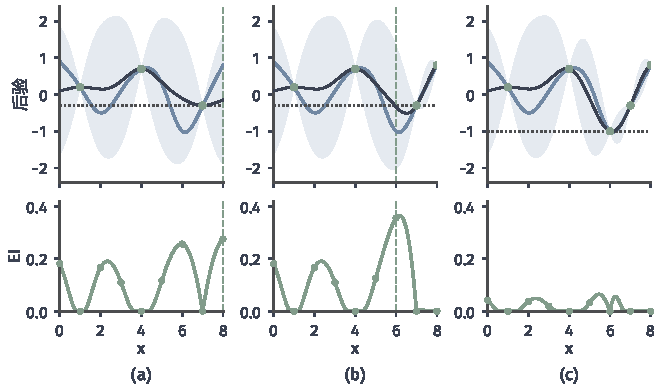
\includegraphics[width=112mm]{figures/05-optimization/05-stochastic-optimization/matplotlib/bo-rounds/figure.pdf}
 \caption{贯穿例的三轮选点。上行：蓝线是目标，深色线是后验均值，浅蓝带是均值上下两倍标准差，点线是当前最好值，绿点是读数。下行：绿线是EI，小点是整数候选上的分数。竖虚线是本轮选中的位置，依次为$x=8$、$x=6$、$x=0$。}
 \label{fig:bo-rounds}
\end{BookInlineFigure}

\subsection{初始设计}
\label{sec:bo-initial-design}

循环开始之前没有任何读数，采集函数没有依据（或者取决于先验，而先验下各处相同）。第一批点因此要在没有反馈的情况下放好，这一步称为\term{初始设计}（initial design）。本小节的问题是：放在哪里，放多少。

先验信息较少时，初始点的任务是覆盖搜索域的不同区域，同时为估计超参数提供不同间距的点对。图~\ref{fig:bo-initial-design}比较了单位方形上放九个点的三种办法。(a)均匀随机的点可能聚集，也可能在某些区域留白。(c)规则网格覆盖整齐，但投影到每个坐标上只有三个不同的值。(b)是\term{拉丁超立方抽样}（Latin hypercube sampling）：把每个坐标轴等分成九格，每行每列恰好放一个点，这样每个坐标轴的投影都分散。网格在高维时会失效，$n$维的$3^n$个格点很快超出预算。

\begin{BookInlineFigure}
 \centering
 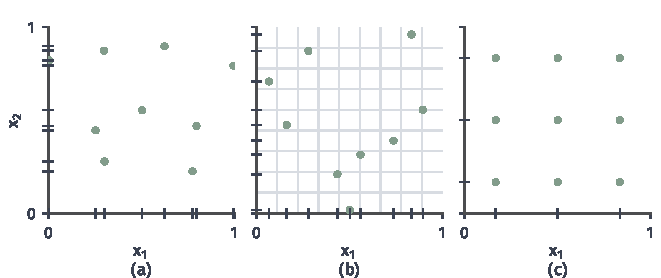
\includegraphics[width=112mm]{figures/05-optimization/05-stochastic-optimization/matplotlib/bo-initial-design/figure.pdf}
 \caption{单位方形上九个初始点的放置（固定随机种子）。(a)均匀随机；(b)拉丁超立方，浅灰线是九等分的格，每行每列恰好一个点；(c)规则网格。坐标轴上的短刻线是点在各坐标的投影，网格投影只有三个不同位置。}
 \label{fig:bo-initial-design}
\end{BookInlineFigure}

初始点不是越多越好，它们挤占后面的定向搜索。图~\ref{fig:bo-initial-budget}在贯穿例上固定总预算$T=8$，改变初始点数，其余用EI选点，统计$300$组随机初始点的平均终端误差。初始点不超过$4$时误差差别很小，因为这里的核是已知的，少量读数已经够用；初始点数达到$7$、$8$时，几乎没有定向评价的机会，平均误差升到$0.085$和$0.241$。

\begin{BookInlineFigure}
 \centering
 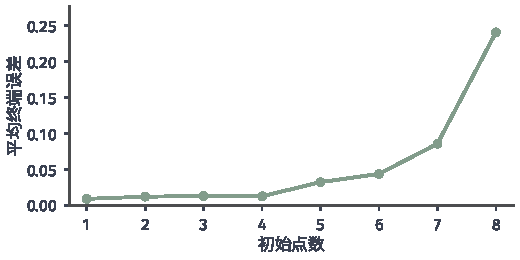
\includegraphics[width=88mm]{figures/05-optimization/05-stochastic-optimization/matplotlib/bo-initial-budget/figure.pdf}
 \caption{初始点数与最终效果。贯穿例，总预算$T=8$，初始点在$0.1$网格上均匀随机选取，其余用EI选点，纵轴是$300$组随机种子下的平均终端误差。初始点数等于$8$时全部预算都用于无反馈的覆盖。}
 \label{fig:bo-initial-budget}
\end{BookInlineFigure}

这个例子的核已知，所以很少的初始点就够了。核的超参数需要估计时，初始点太少会使边缘似然不可靠，代理在开始几轮可能严重失真，常见的经验是取搜索维数的若干倍（如$10n$），但这只是经验，总预算很小时要相应减少。

\subsection{采集函数求解}
\label{sec:bo-inner}

每轮要解一个内层优化问题：
\begin{equation}
 \bm{x}_{t+1}\in\argmax_{\bm{x}\in\bm{C}}\alpha_t(\bm{x}).
 \label{eq:bo-inner}
\end{equation}
它与外层目标的代价完全不同：$\alpha_t$是一个有解析式、可以快速求值的函数。但它一般不是凹函数，而且常有多个峰，本小节的问题就是怎样可靠地求它的最大点。

\paragraph{可用的导数}
真实目标不提供导数，但采集函数的导数完全来自代理。由式~\eqref{eq:bo-ei-derivatives}和链式法则，在$s_t(\bm{x})>0$的位置，
\begin{equation}
 \nabla\mathrm{EI}_t(\bm{x})=-\Phi(z)\nabla m_t(\bm{x})+\phi(z)\nabla s_t(\bm{x}).
 \label{eq:bo-ei-gradient}
\end{equation}
由式~\eqref{eq:bo-post-mean}和式~\eqref{eq:bo-post-cov}，令$\nabla\bm{k}_t(\bm{x})$表示$\bm{k}_t$对$\bm{x}$的Jacobi矩阵，并设核满足$k(\bm{x},\bm{x})$为常数，
\begin{align}
 \nabla m_t(\bm{x})&=\nabla\bm{k}_t(\bm{x})^\top\bm{A}_t^{-1}(\bm{y}_t-\bm{m}_{0,t})+\nabla m_0(\bm{x}),
 \label{eq:bo-grad-m}\\
 \nabla s_t(\bm{x})&=-\frac{\nabla\bm{k}_t(\bm{x})^\top\bm{A}_t^{-1}\bm{k}_t(\bm{x})}{s_t(\bm{x})}.
 \label{eq:bo-grad-s}
\end{align}
这些导数只要求核可导，不要求目标$f$可导。

用只有一个读数$F(7)=-0.3$的情形验算一下。取$x=6$，$b=-0.3$，则
\[
 k(6,7)=\tfrac12,\qquad \frac{\mathrm{d}k}{\mathrm{d}x}=-2\ln2\,(x-7)\,k\approx0.693.
\]
后验均值与方差及其导数是
\[
 m=-0.15,\quad m'\approx-0.208,\quad s\approx0.866,\quad s'\approx-0.400,
\]
其中$s'$由$(s^2)'=-2kk'$算得。这里$z\approx-0.173$，$\Phi(z)\approx0.431$，$\phi(z)\approx0.393$，代入式~\eqref{eq:bo-ei-gradient}，
\[
 \frac{\mathrm{d}\mathrm{EI}}{\mathrm{d}x}\approx0.431\times0.208-0.393\times0.400\approx-0.067.
\]
导数为负，说明从$x=6$向$x=7$走时，方差减小的损失超过了均值降低的收益。

\paragraph{多起点、候选筛选与随机搜索}
一个起点的局部上升只能到达它所在的峰。常用的做法是多起点局部优化：取一批起点，通常先在大量候选上计算$\alpha_t$，挑其中分数高的作起点，再用带约束的拟牛顿法作局部上升。也可以直接在候选集上比较分数，或用第~\ref{chap:random-search}章的随机搜索方法。这些方法都只求一个便宜函数的最大值，不增加昂贵评价。

图~\ref{fig:bo-inner-multistart}是贯穿例$t=5$时的情形。八个等距起点沿EI爬升，到达了四个不同的局部最大点，取值约为$0.042,0.049,0.065,0.057$，全局最大点在$x\approx5.46$。起点$x=7.5$附近EI几乎为零，梯度也几乎为零，上升根本走不动，这是平坦区域的常见困难，通常的对策是对EI取对数后再优化。

\begin{BookInlineFigure}
 \centering
 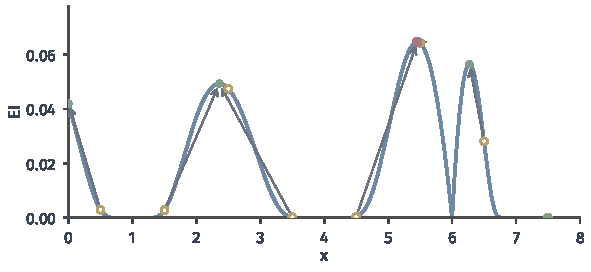
\includegraphics[width=100mm]{figures/05-optimization/05-stochastic-optimization/matplotlib/bo-inner-multistart/figure.pdf}
 \caption{内层问题的多起点求解。贯穿例$t=5$，蓝线是EI，黄色空心点是八个起点，灰色箭头是数值上升的起止，绿点是到达的局部最大点，红点是其中最好的点$x\approx5.46$。}
 \label{fig:bo-inner-multistart}
\end{BookInlineFigure}

对比这一轮的正文计算，整数候选集上的最大值是$\mathrm{EI}_5(0)\approx0.042$，而连续域上的最大点在$x\approx5.46$，取值$0.065$。内层问题的解法确实会改变外层的选点，这说明内层近似不是无关紧要的细节。内层近似求解也不自动得到采集函数的全局最优点；若分析某种算法的性质时假设了内层精确求解，实际运行时这个假设需要另外检查。

\subsection{观测更新}
\label{sec:bo-observation-update}

选定位置并运行真实评价之后，要回答的问题是：新读数应当怎样进入模型。

把新读数和它的噪声信息加入$\mathcal{D}_t$后，式~\eqref{eq:bo-update-mean}、式~\eqref{eq:bo-update-cov}更新候选点上的后验。若在搜索域的任意点上重新计算，需要更新Cholesky分解，也可以增量进行。设$\bm{A}_t=\bm{L}_t\bm{L}_t^\top$，新矩阵的因子只在末尾加一行：
\begin{equation}
 \bm{L}_{t+1}=\begin{bmatrix}\bm{L}_t&\bm{0}\\\bm{\ell}^\top&d\end{bmatrix},
 \label{eq:bo-chol-update}
\end{equation}
其中
\[
 \bm{\ell}=\bm{L}_t^{-1}\bm{k}_t(\bm{x}^+),\qquad
 d^2=k(\bm{x}^+,\bm{x}^+)+\tau^2-\bm{\ell}^\top\bm{\ell}.
\]
求$\bm{\ell}$只需一次前代，所以这一步需要$O(t^2)$次运算，不必花$O(t^3)$次重新分解。$d^2$恰好是新读数的预测方差$v$。如果这一轮重新估计了超参数，核矩阵整体改变，增量更新就不再适用，要重新分解。

这里要保留完整的历史，而不是只记住当前最好值。只记$b_t$的做法在第一轮之后只知道“最好值仍是$-0.3$”，看不到$x=8$的读数，也算不出$\mathrm{EI}_4(6)$从$0.257$升到$0.356$这个变化。未获改进的观测也有信息，它改变相关区域的预测，进而改变后续查询的价值。第一轮的$x=8$正是这种情形，图~\ref{fig:bo-rounds}(a)到(b)的变化说明了它的作用。

\section{含噪观测}
\label{sec:bo-noisy}

到目前为止，读数都是函数值本身。真实的仿真或实验常常带噪声，同一个$\bm{x}$运行两次，结果不一样。设
\begin{equation}
 y_i=f(\bm{x}_i)+\varepsilon_i,
 \label{eq:bo-noisy-obs}
\end{equation}
其中$\varepsilon_i$相互独立，服从均值为$0$、方差为$\tau^2$的高斯分布。此时要分清两个对象：未知但固定的函数值$f(\bm{x})$，和每次测量才产生的随机读数$y$。这就需要回答：噪声使前面哪些做法失效，选点规则应当怎样改？

\subsection{两种预测方差}
\label{sec:bo-noise-variances}

噪声出现后，“这个位置的不确定性”有两种说法。一种是对潜在函数值$F(\bm{x})$的不确定，后验方差为$s_t^2(\bm{x})$。另一种是对下一次读数$y$的不确定，这要多加一份测量噪声。独立噪声方差为$\tau^2$时，
\begin{equation}
 \operatorname{Var}(y\mid\mathcal{D}_t,\bm{x})=s_t^2(\bm{x})+\tau^2.
 \label{eq:bo-pred-var}
\end{equation}
这里用到$y=F(\bm{x})+\varepsilon$，新的$\varepsilon$与$F$及已有数据独立，方差相加。

图~\ref{fig:bo-noise-bands}展示了两者的差别。浅蓝带表示潜在函数值的范围，紫色虚线表示下一次读数可能的范围。读数点不再落在后验均值上，模型会把读数“往回拉”，因为它知道读数里含有噪声；即使在读数附近，后验方差也不为零。

\begin{BookInlineFigure}
 \centering
 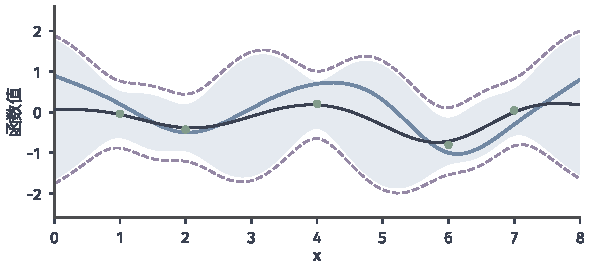
\includegraphics[width=100mm]{figures/05-optimization/05-stochastic-optimization/matplotlib/bo-noise-bands/figure.pdf}
 \caption{两种预测方差。噪声标准差$\tau=0.3$，绿点是五个含噪读数（固定随机种子）。蓝线是目标，深色线是后验均值，浅蓝带是$m_t\pm2s_t$，紫虚线是$m_t\pm2\sqrt{s_t^2+\tau^2}$。}
 \label{fig:bo-noise-bands}
\end{BookInlineFigure}

在同一位置重复读数，能减少的是第一种方差。设先验方差为$1$，$\tau^2=0.09$，在$x$处读$n$次，由定理~\ref{thm:bo-posterior}，
\[
 s^2(x)=\frac{\tau^2}{n+\tau^2}.
\]
$n=1,4,9$时，$s^2$依次约为
\[
 0.083,\qquad 0.022,\qquad 0.010.
\]
而下一次读数的方差始终比$s^2$多$0.09$，这一份噪声不会因观测而消失。观测多了，我们越来越清楚$f(x)$是多少，但下一次测量出来的数照样抖动。

\paragraph{方差能否只减不增}
超参数固定时，由更新式~\eqref{eq:bo-update-cov}，
\[
 s_{t+1}^2(\bm{x})=s_t^2(\bm{x})-\frac{c_t(\bm{x},\bm{x}^+)^2}{s_t^2(\bm{x}^+)+\tau^2}\leq s_t^2(\bm{x}),
\]
新增观测不会使潜在值的后验方差增大。这个结论只在模型固定时成立。

重新拟合超参数就可能使方差增大。设$k=\sigma^2k_0$，其中$k_0$是贯穿例的核，幅度$\sigma^2$用边缘似然估计，无噪声。只有$x=1$的读数$1$时，估计值$\widehat{\sigma}^2=1$，于是
\[
 s^2(2)=\widehat{\sigma}^2\cdot\tfrac34=0.75.
\]
再评价相距很远的$x=6$，读到$3$，两点几乎不相关，幅度估计变为
\[
 \widehat{\sigma}^2\approx\frac{1^2+3^2}{2}=5,
\]
于是$s^2(2)\approx3.75$，反而变大了。新读数告诉模型“函数的波动比原来以为的大”，模型便下调了之前的把握。这两种情形都和“消除下一次测量的噪声”无关。

\subsection{含噪选点}
\label{sec:bo-noisy-selection}

\paragraph{最低读数可能只是运气好}
式~\eqref{eq:bo-incumbent}的$b_t$在含噪时不能直接用读数的最小值代替。读数的最小值常常是噪声偏向负方向的那一次。图~\ref{fig:bo-noise-incumbent}上半部分中，六个读数里最低的是$x=2$处的$-0.95$（红圈），但$f(2)=-0.5$，真实更好的$x=6$只读到$-0.55$，因为那次噪声是正的。

用含噪的最低读数做阈值，会把门槛设得过低，好像已经找到一个其实并不存在的好结果。一种改法是把阈值换成已评价点上的最小后验均值，这样噪声被模型部分平滑了；这是一种具体的近似规则，并不等于对真实阈值作了正确处理。

\paragraph{含噪期望改进}
更一致的做法是承认阈值也不确定。真实的“已评价最好值”是$\min_iF(\bm{x}_i)$，它是随机的。把它和候选点放在同一个后验下，定义\term{含噪期望改进}（noisy expected improvement，NEI）：
\begin{equation}
 \mathrm{NEI}_t(\bm{x})=\mathbb{E}\Bigl[\bigl(\min_{i\leq t}F(\bm{x}_i)-F(\bm{x})\bigr)_+\,\Bigm|\,\mathcal{D}_t\Bigr].
 \label{eq:bo-nei}
\end{equation}
这里的期望对$F(\bm{x}_1),\ldots,F(\bm{x}_t),F(\bm{x})$的\emph{联合}后验取，协方差不能丢：若候选点与某已评价点强相关，两者的差就不会太大。一般情形下没有闭式，常用的做法是抽取这$t+1$个值的联合后验样本，取平均。

\paragraph{例：只有一个评价点}
只有一个评价点时，NEI可以手算。设$\tau^2=0.09$，在$x=2$读到$y=-0.5$，候选为$x=4$。相关系数$\rho=1/16$，由定理~\ref{thm:bo-posterior}，
\[
 \begin{aligned}
 F(2)\mid\mathcal{D}:&\ \text{均值}\ -0.459,\quad\text{方差}\ 0.083,\\
 F(4)\mid\mathcal{D}:&\ \text{均值}\ -0.029,\quad\text{方差}\ 0.996,
 \end{aligned}
\]
两者的后验协方差约为$0.005$。

把$D=F(2)-F(4)$看成一个高斯量，其均值与方差为
\[
 \mathbb{E}D\approx-0.430,\qquad \operatorname{Var}D\approx0.083+0.996-2\times0.005\approx1.069.
\]
由于$\mathrm{NEI}=\mathbb{E}D_+$，用式~\eqref{eq:bo-ei}的同一积分，标准化后$u\approx-0.416$，
\[
 \mathrm{NEI}\approx-0.430\,\Phi(u)+1.034\,\phi(u)\approx0.233.
\]

同一位置上，以读数$-0.5$为阈值的EI约为$0.206$，以后验均值$-0.459$为阈值的EI约为$0.220$。NEI最大，因为它考虑了阈值$F(2)$自身的不确定性：阈值可能比后验均值高，候选点就更容易改进。

图~\ref{fig:bo-noise-incumbent}下半部分比较了三种做法。阈值用最低读数时，门槛被噪声压低，除$x=2$附近外，分数都比另外两条线小（黄线）；阈值用最小后验均值时，$x=2$处仍有一个较高的峰，因为最小后验均值落在$x=2$（紫虚线）；NEI在已评价的$x=2$附近凹下去，并把价值分到其他地方（绿线）。

\begin{BookInlineFigure}
 \centering
 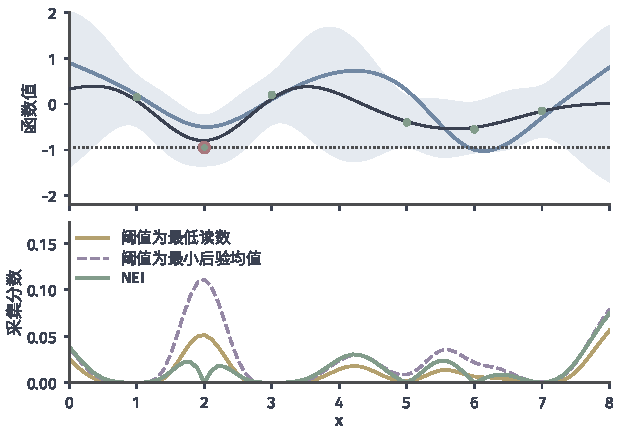
\includegraphics[width=105mm]{figures/05-optimization/05-stochastic-optimization/matplotlib/bo-noise-incumbent/figure.pdf}
 \caption{最低读数与含噪选点。上：$\tau=0.3$，六个读数，噪声依次取为$-0.05,-0.45,0.1,-0.7,0.45,0.15$（手工给定，用以突出$x=2$的偶然低值），红圈是最低读数，点线是其数值；蓝线是目标，深色线是后验均值。下：三种采集分数，NEI由$40000$个联合后验样本估计。}
 \label{fig:bo-noise-incumbent}
\end{BookInlineFigure}

NEI和知识梯度衡量的东西不同。NEI问的是“潜在函数值能否低于已评价点”，KG问的是“这次观测后，最终推荐的价值能改善多少”。无噪声时前者是EI的直接推广，后者需要再做一次前瞻。两者都在含噪时有定义，下一节就会看到它们对“重复测量”的回答相反。

\subsection{重复评价}
\label{sec:bo-replicates}

含噪时一个自然的动作是把同一个位置再测一次。这样做有用吗？按潜在改进的定义，答案是否定的。若$\bm{x}$恰好是某个已评价点$\bm{x}_j$，则$\min_iF(\bm{x}_i)\leq F(\bm{x}_j)$，改进量恒为$0$，所以
\begin{equation}
 \mathrm{NEI}_t(\bm{x}_j)=0.
 \label{eq:bo-nei-zero}
\end{equation}
图~\ref{fig:bo-noise-incumbent}的绿线在$x=2$处贴到零，正是这个原因。NEI从定义上就看不到复测的价值，因为复测不产生新位置，只是更清楚地认识旧位置。

复测的价值要由信息更新的准则来衡量。式~\eqref{eq:bo-kg}的KG没有这种限制。设两个候选A、B，$F(\text{A})$的后验均值$0$，方差$s^2=0.04$，$F(\text{B})$的后验均值$0.1$，两者后验独立，测量噪声$\tau^2=0.09$。当前推荐A。再测一次A后，由式~\eqref{eq:bo-kg-update}，
\[
 \widetilde{\sigma}=\frac{0.04}{\sqrt{0.04+0.09}}\approx0.111.
\]

新的推荐价值是$\min\{0.111Z,\ 0.1\}$，标准化的间距$u=0.1/0.111\approx0.901$。于是
\[
 \begin{aligned}
 \mathrm{KG}&=0-\mathbb{E}\min\{0.111Z,\,0.1\}\\
 &=0.111\bigl(\phi(u)-u(1-\Phi(u))\bigr)\approx0.011.
 \end{aligned}
\]
这个值大于$0$：再测一次A可能发现它其实比B差，从而改变推荐。

\paragraph{该重复多少次}
重复次数取决于要区分的差距和噪声。设两个候选的真实差距为$\Delta$，噪声标准差为$\tau$，各读$n$次后比较平均读数，选对的概率为
\begin{equation}
 \mathbb{P}(\text{选对})=\Phi\left(\frac{\Delta\sqrt{n}}{\tau\sqrt{2}}\right).
 \label{eq:bo-correct-selection}
\end{equation}
这里用到两个平均读数之差服从$N(\Delta,2\tau^2/n)$。取$\Delta=0.2$，$\tau=0.3$，$n=1,4,9$时的概率依次为
\[
 0.681,\qquad 0.827,\qquad 0.921.
\]
可见差距接近噪声水平时，一次测量基本在碰运气。代价接近的候选之间要靠复测来决定，能否负担这个复测要由预算决定。

最后要留意单次异常读数。一个比预期低$3$倍标准差的读数，可能是噪声，也可能是模型错了，比如该位置附近有一个模型没想到的窄谷。留一残差~\eqref{eq:bo-loo}只能发现它异常，不能告诉我们原因。在同一位置复测可以帮助区分：回到预期附近，说明是噪声；复测仍然很低，说明应当修改模型的设定。

\section{约束下的选点}
\label{sec:bo-constraints}

前面的搜索域是已知的。实际问题常带约束，其中有两类要分开。已知且容易判断的约束，比如参数上下限、整数限制，在内层问题~\eqref{eq:bo-inner}里直接限定搜索域即可，真实评价都发生在可行点上。另一类是未知且昂贵的约束：例如“峰值应力不超过上限”，只有仿真运行结束才知道是否满足。

设目标损失和性能上限都要运行才能测得，问题写成
\begin{equation}
 \min_{\bm{x}\in\bm{C}}\ f(\bm{x})\quad\text{s.t.}\quad g_j(\bm{x})\leq0,\ \ j=1,\ldots,m.
 \label{eq:bo-constrained}
\end{equation}
一个候选点的目标值可以很好，却是不可行的。怎样让未知约束进入选点，而“最终可行”和“每次试验都可行”又有什么不同？

\subsection{可行概率}
\label{sec:bo-feasibility}

对每个$g_j$也用一个代理建模，得到后验$G_j$。候选点满足全部约束的后验概率称为可行概率。若当前后验下各约束相互独立，并且第$j$个约束的后验为$N(m_j(\bm{x}),s_j^2(\bm{x}))$，$s_j(\bm{x})>0$，则
\begin{equation}
 \mathrm{PF}_t(\bm{x})=\prod_{j=1}^m\Phi\left(\frac{-m_j(\bm{x})}{s_j(\bm{x})}\right).
 \label{eq:bo-feasible-prob}
\end{equation}

阈值$b_t$也要相应改变：它是已评价点中\emph{可行者}的最好读数。一个不可行点读数再低，也不能作为改进的基准。可行改进的期望是
\[
 \mathbb{E}\Bigl[\bigl(b_t-F(\bm{x})\bigr)_+\,\mathbf{1}\{G_j(\bm{x})\leq0,\ \forall j\}\,\Bigm|\,\mathcal{D}_t\Bigr].
\]
其中$\mathbf{1}\{\cdot\}$表示事件成立时取$1$、否则取$0$。

当前后验下，目标改进与各约束事件相互独立时，乘积的期望等于期望的乘积，所以
\begin{equation}
 \mathrm{cEI}_t(\bm{x})=\mathrm{EI}_t(\bm{x})\cdot\mathrm{PF}_t(\bm{x}).
 \label{eq:bo-cei}
\end{equation}
独立这个条件不能省略。若目标和约束由同一个物理量驱动，相关性强，式~\eqref{eq:bo-cei}就不再是可行改进的期望，需要联合积分。

\paragraph{贯穿例}
在贯穿例上加一个约束$g(x)=(x-4.5)/4\leq0$，算法只能通过评价得知它的值，用同样的核建模。三个读数为$g(1)=-0.875$，$g(4)=-0.125$，$g(7)=0.625$。$x=7$不可行，尽管它读数最低，因此可行最好值是
\[
 b_3=f(1)=0.2.
\]

计算$x=2$的$\mathrm{cEI}$。目标的后验$m=0.143$，$s=0.864$，代入式~\eqref{eq:bo-ei}得$\mathrm{EI}\approx0.374$。约束的后验$m_g\approx-0.445$，$s_g\approx0.864$，可行概率为
\[
 \Phi(0.445/0.864)=\Phi(0.515)\approx0.697.
\]
于是
\[
 \mathrm{cEI}(2)\approx0.374\times0.697\approx0.261.
\]

表~\ref{tab:bo-cei}列出几个候选的结果。不考虑约束的EI选择$x=8$，加上可行概率之后，右侧候选的分数大幅下降，最大值转到$x=0$。图~\ref{fig:bo-constrained}画出了完整的曲线：$x=7$的EI是$0.5$，但$g(7)>0$已知，cEI为$0$。

\begin{BookInlineTable}
 \centering
 \caption{贯穿例的约束选点，$t=3$，$b_3=0.2$（可行读数中最小的）。}
 \label{tab:bo-cei}
 \begin{tabular}{cccccc}
 \toprule
 $x$&$\mathrm{EI}$&$m_g$&$s_g$&$\mathrm{PF}$&$\mathrm{cEI}$\\
 \midrule
 0&0.398&$-0.437$&0.866&0.693&$\mathbf{0.276}$\\
 2&0.374&$-0.445$&0.864&0.697&0.261\\
 6&0.520&0.305&0.864&0.362&0.188\\
 8&0.549&0.313&0.866&0.359&0.197\\
 \bottomrule
 \end{tabular}
\end{BookInlineTable}

\begin{BookInlineFigure}
 \centering
 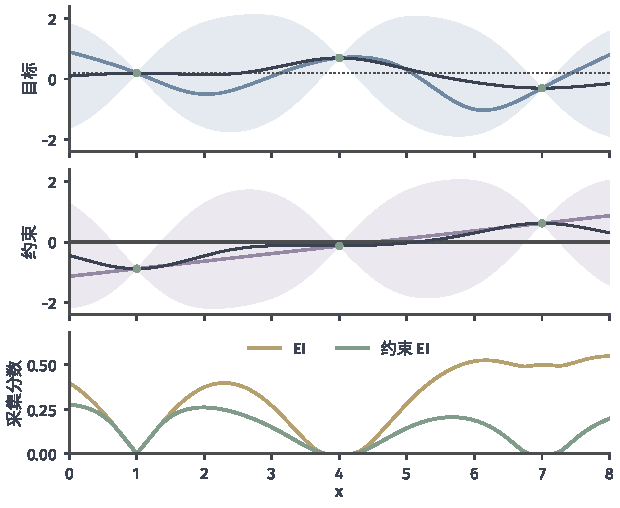
\includegraphics[width=105mm]{figures/05-optimization/05-stochastic-optimization/matplotlib/bo-constrained/figure.pdf}
 \caption{未知约束下的选点。上：目标的后验，蓝线是目标，点线是当前可行最好值$b_3=0.2$。中：约束的后验，紫线是真实的$g$，深灰线是边界$g=0$。下：黄线是不考虑约束的EI，绿线是约束EI，$x=7$处EI较大但已知不可行，约束EI为$0$。}
 \label{fig:bo-constrained}
\end{BookInlineFigure}

\paragraph{还没有可行点时}
读数中若没有可行点，$b_t$没有定义，EI也就无从算起。这时需要先规定一个寻找可行点的准则，最常见的是选$\mathrm{PF}_t(\bm{x})$最大的位置，等找到第一个可行点后，再转入$\mathrm{cEI}$。

\subsection{评价的可行性}
\label{sec:bo-eval-feasibility}

约束有两种含义，到这里还没有分开：一种要求\emph{最终推荐解}可行，中途的试验可以不可行；另一种要求\emph{每次试验}都不能违反约束，比如试验中的设备一旦过热就会损坏。前面的$\mathrm{cEI}$只处理第一种，它会故意到不可行区域采样，以弄清边界。

第二种要求要严格得多。单个点的后验可行概率高并不够用。设每轮选的点可行概率都是$0.95$，假设各轮近似独立，$20$轮全部可行的概率只有
\[
 0.95^{20}\approx0.36.
\]
要保证每次试验都可行，需要三样额外的东西：能把模型与真实约束联系起来的假设（例如$g$确实来自这个高斯过程，或有已知的Lipschitz常数）、至少一个已知可行的初始点、以及保守的选点规则。

图~\ref{fig:bo-safe-set}展示了一种保守的做法：以$g$的后验上界$m_g+2s_g\leq0$定义\emph{安全集}，每轮只在安全集内选点，示例中都取安全集的右端点。这里的约束是前面的$g(x)=(x-4.5)/4$，初始已知$x=1$可行。安全集三轮依次为
\[
 [0.66,1.34],\qquad[0.48,1.76],\qquad[0.32,2.28].
\]
这样的扩张靠边界附近的试验逐步推进，很慢，也可能永远到不了与初始点隔开的另一块可行区域。而且上界中的系数$2$是单点意义上的；要保证所有试验都安全，系数还须按第~\ref{sec:bo-guarantees}节的方式放大。

\begin{BookInlineFigure}
 \centering
 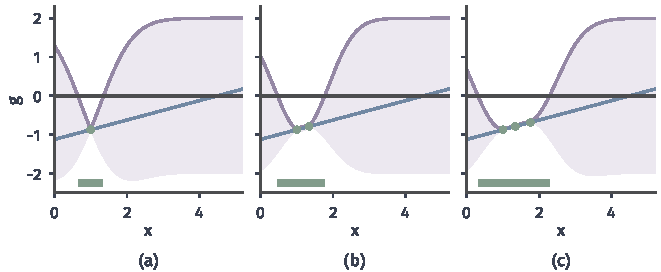
\includegraphics[width=112mm]{figures/05-optimization/05-stochastic-optimization/matplotlib/bo-safe-set/figure.pdf}
 \caption{保守选点下安全集的扩张。蓝线是真实约束$g(x)=(x-4.5)/4$，深灰线是边界，浅紫带是后验$m_g\pm2s_g$，紫线是上界$m_g+2s_g$，绿点是已做的试验，底部绿色粗线是上界不超过$0$的安全集。(a)、(b)、(c)依次是第一、二、三轮。}
 \label{fig:bo-safe-set}
\end{BookInlineFigure}

\section{批量评价}
\label{sec:bo-batch}

到现在为止，算法一次只运行一个试验，等结果回来再决定下一个。如果手上有两台机器，就可以同时跑两个。于是要问：多个试验同时运行时，候选应当怎样选，尚未返回的试验又该如何处理？

并行带来的好处和代价都很具体。图~\ref{fig:bo-parallel-timeline}比较了完成四次评价的三种方式。(a)一台机器逐个运行，每次选点都能用上之前全部结果，总时长最长。(b)两台机器同步批量运行，时长减半，但第$2$次评价没有用上第$1$次的结果。(c)两台机器异步运行，耗时不等，一台空出来就立刻派新试验，此时另一台上的试验还没有结果。

\begin{BookInlineFigure}
 \centering
 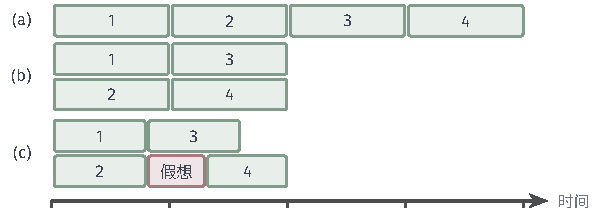
\includegraphics[width=102mm]{figures/05-optimization/05-stochastic-optimization/tikz/bo-parallel-timeline/figure.pdf}
 \caption{四次评价的三种安排，横轴是时间，每个绿框是一次评价，数字是选点顺序。(a)串行。(b)两台机器的同步批量。(c)异步，两台机器上的评价耗时不等，第$3$次选点时第$2$次评价还在运行，第$2$次评价后段的红框表示这段时间里结果尚未返回，第$3$次选点的计算对它使用假想结果，它不是观测。}
 \label{fig:bo-parallel-timeline}
\end{BookInlineFigure}

\subsection{联合选点}
\label{sec:bo-joint-batch}

一次选$q$个点时，最容易想到的做法是取单点采集分数最高的$q$个位置。问题在于这$q$个点常常挤在一个峰上。图~\ref{fig:bo-batch-joint}是贯穿例$t=4$时、在$0.25$网格上选两点的结果：单点EI最高的两点是$x=6.25$和$x=6$（黄方块），它们几乎重复。

应当衡量的是整批的价值。无噪声时，一批候选$\bm{x}_1',\ldots,\bm{x}_q'$的批量期望改进（q-EI）是
\begin{equation}
 \mathrm{qEI}_t(\bm{x}_1',\ldots,\bm{x}_q')=\mathbb{E}\Bigl[\bigl(b_t-\min_{j\leq q}F(\bm{x}_j')\bigr)_+\,\Bigm|\,\mathcal{D}_t\Bigr].
 \label{eq:bo-qei}
\end{equation}
期望对这$q$个函数值的联合后验取，所以候选点之间的相关性直接影响整批的价值。

\paragraph{相关性怎样影响整批价值}
用两个候选说清楚。设$b_t=0$，两者的后验均为$N(0,1)$，相关系数为$\rho$。单点EI都是$\phi(0)\approx0.399$，这里记$X=-F(\bm{x}_1')$，$Y=-F(\bm{x}_2')$，则
\[
 \mathrm{qEI}=\mathbb{E}\max\{0,X,Y\}.
\]

三个数$0,X,Y$从小到大排列为$U_1\leq U_2\leq U_3$。对$a,b,c$两两取最大值再求和，结果等于最大数的两倍加中间数，所以
\[
 2U_3+U_2=\max\{0,X\}+\max\{0,Y\}+\max\{X,Y\}.
\]

$(X,Y)$与$(-X,-Y)$同分布，取负号后最小的变成最大的，中间的仍是中间的，并且符号相反，所以$\mathbb{E}U_2=0$。两边取期望，再用
\[
 \mathbb{E}\max\{0,X\}=\frac1{\sqrt{2\pi}},\qquad
 \mathbb{E}\max\{X,Y\}=\sqrt{\frac{1-\rho}{\pi}},
\]
其中第二式来自$\max\{X,Y\}=(X+Y+\lvert X-Y\rvert)/2$和$X-Y\sim N(0,2(1-\rho))$，得到
\begin{equation}
 \mathrm{qEI}=\frac1{\sqrt{2\pi}}+\frac12\sqrt{\frac{1-\rho}{\pi}}.
 \label{eq:bo-qei-two}
\end{equation}

取$\rho=1,0.5,0$时，$\mathrm{qEI}$依次约为
\[
 0.399,\qquad 0.598,\qquad 0.681.
\]
两点完全相同时，第二个点没有价值，整批的价值就是单点EI；越不相关，第二个点带来的额外机会越大。但即使独立，第二个点的边际价值也小于单点EI的$0.399$，因为它和第一个点要竞争同一个“成为更好者”的位置。所以把单点分数相加不等于整批的价值。

回到贯穿例。单点EI最高的两点，整批$\mathrm{qEI}\approx0.407$，两点的单点EI之和却是$0.719$。$0.25$网格上最好的一对是$x=2.25$和$x=6.25$（绿点），整批$\mathrm{qEI}\approx0.487$，第二个点不再去挤第一个峰。

\begin{BookInlineFigure}
 \centering
 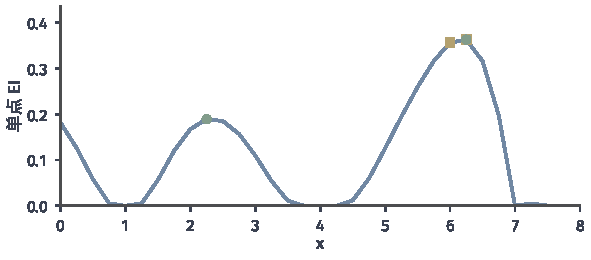
\includegraphics[width=100mm]{figures/05-optimization/05-stochastic-optimization/matplotlib/bo-batch-joint/figure.pdf}
 \caption{一次选两点。贯穿例$t=4$，$0.25$网格，蓝线是单点EI。黄方块是单点分数最高的两点（$x=6$与$x=6.25$），绿点是使$\mathrm{qEI}$最大的两点（$x=2.25$与$x=6.25$），后者由$40000$个公共后验样本估计，$x=6.25$的绿点与黄方块重合。}
 \label{fig:bo-batch-joint}
\end{BookInlineFigure}

$q$大时联合优化是$qn$维的内层问题，闭式也不再存在，通常用联合样本近似期望，再用重参数化式~\eqref{eq:bo-joint-sample}对候选位置求梯度。

\subsection{未完成的评价}
\label{sec:bo-pending}

异步运行时，一台机器空出来要立刻派新试验，而另一台上的试验还没有结果。本小节的问题是：尚未返回的试验，在选点计算中该如何对待。

忽略它们不对。忽略后下一轮的选择可能恰好与运行中的位置重复。图~\ref{fig:bo-pending-fantasy}中，若$x=6$的试验正在运行，黄线仍在$x=6$处给出高分。把运行中的位置也算作数据，就要用读数，而读数还没有。

正确做法是对可能的结果作平均。设运行中的位置为$\bm{x}_{\mathrm{p}}$，结果按当前预测分布取值，定义
\begin{equation}
 \bar\alpha_t(\bm{x})=\mathbb{E}_{y_{\mathrm{p}}}\bigl[\alpha_t\bigl(\bm{x}\mid\mathcal{D}_t\cup\{(\bm{x}_{\mathrm{p}},y_{\mathrm{p}})\}\bigr)\bigr],
 \label{eq:bo-fantasy}
\end{equation}
其中期望按$y_{\mathrm{p}}\sim N(m_t(\bm{x}_{\mathrm{p}}),s_t^2(\bm{x}_{\mathrm{p}})+\tau^2)$计算，实际常用少量抽样近似。

这里用于计算的$y_{\mathrm{p}}$称为假想结果，它不是观测，不能写进$\mathcal{D}_t$，算完就丢弃。真实结果返回后，仍须用真实读数更新后验。

看$\bm{x}_{\mathrm{p}}=6$的情形（无噪声，$t=3$）。对任何假想结果，$x=6$处的后验方差都变为零，改善量都是$0$，平均之后$\bar\alpha_3(6)=0$。图中绿线在$x=6$降到零，附近也被压低，$x=8$的分数从$0.276$降到约$0.233$，因为阈值在有些假想情形下变低了。这样下一台机器不会与运行中的试验重复。

\begin{BookInlineFigure}
 \centering
 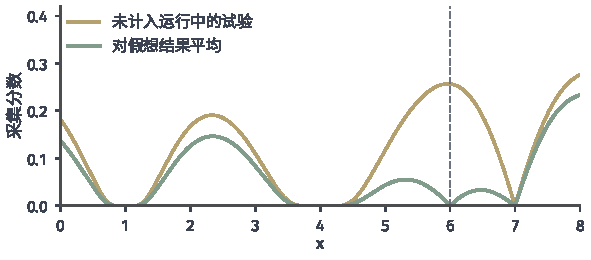
\includegraphics[width=100mm]{figures/05-optimization/05-stochastic-optimization/matplotlib/bo-pending-fantasy/figure.pdf}
 \caption{对运行中试验的处理。贯穿例$t=3$，竖虚线是运行中的位置$x=6$。黄线是不考虑运行中试验的EI，绿线是对假想结果取平均之后的EI（$201$个等分位假想读数）。绿线在$x=6$处为$0$。}
 \label{fig:bo-pending-fantasy}
\end{BookInlineFigure}

\section{预算与结果评价}
\label{sec:bo-budget}

循环总要结束。本节回答最后几个问题：预算究竟应当怎样计算，什么时候停止，交出什么，这个结果好到什么程度，以及哪些结论有理论保证。这些问题放在一起，是因为比较方法时必须固定同一套口径：搜索域、可用信息和预算。

\subsection{评价成本}
\label{sec:bo-cost}

不同位置的运行代价可能差别很大，比如某个参数越大，仿真越慢。一种常见的调整是除以预测成本$\widehat{c}(\bm{x})$，选单位成本的改进最大的点：
\begin{equation}
 \alpha_t^{\mathrm{cost}}(\bm{x})=\frac{\mathrm{EI}_t(\bm{x})}{\widehat{c}(\bm{x})}.
 \label{eq:bo-cost-ei}
\end{equation}
这只是一种特定的预算策略，它不自动最优地分配剩余总预算。下面的小例子说明这一点。剩余预算是$9$，候选A成本$1$、预期收益$2$，候选B成本$9$、预期收益$16.2$。单位成本的收益分别为
\[
 2,\qquad1.8.
\]
按单位成本选A，用掉$1$后，剩余$8$不够运行B，总收益只有$2$；一开始就选B，总收益为$16.2$。贪心比值没有考虑“预算够不够下一个”。

时间也要分开算。评价次数少不等于总耗时短。表~\ref{tab:bo-time}区分三种常被混用的时间。若一次评价只要$1$秒，贝叶斯优化的内层计算可能远超评价本身，这时随机搜索更快；若一次评价要$1$小时，每轮花$1$分钟做选点几乎没有成本。比较方法时只比较外层迭代数，等于默认了内层计算不要钱。

\begin{BookInlineTable}
 \centering
 \caption{三种时间口径，$c_i$是第$i$次评价的耗时，$a_i$是第$i$轮算法计算的耗时，$q$是并行的机器数。}
 \label{tab:bo-time}
 \begin{tabular}{ll}
 \toprule
 口径&计算方式\\
 \midrule
 串行总耗时&$\sum_i(c_i+a_i)$\\
 并行等待时间&约$\sum_i c_i/q$，耗时不等时更长\\
 算法自身计算时间&$\sum_i a_i$，高斯过程每轮约$O(t^3)$\\
 \bottomrule
 \end{tabular}
\end{BookInlineTable}

\subsection{停止与推荐}
\label{sec:bo-stopping}

最直接的停止条件是预算耗尽，这不需要任何模型。也可以在采集分数很小时提前停止，例如$\max_{\bm{x}}\mathrm{EI}_t(\bm{x})$低于一个阈值。这种停止依赖两件事：代理是否可信，以及内层求解是否找到了采集函数的最大点。第~\ref{sec:bo-model-specification}节中$\ell=3$的模型在$x=6$处方差极小，据此计算的EI也很小，算法就会在没有真正探索的情况下停下来。

推荐规则要在运行前说定。无噪声时可以返回已评价的最好点，贯穿例中就是$\widehat{x}_6=6$。含噪时，已评价的最好读数可能只是运气，通常用后验均值提出候选，例如选$\min_{\bm{x}}m_T(\bm{x})$的位置，再用预留的预算在候选处复测。最后报告采用的推荐规则，以及推荐值的不确定性，不只报告一个数字。

\subsection{推荐误差}
\label{sec:bo-regret}

交出$\widehat{\bm{x}}_T$后，自然要问它离最好的结果有多远。记$f^\star=\inf_{\bm{x}\in\bm{C}}f(\bm{x})$，用\term{简单遗憾}（simple regret）$f(\widehat{\bm{x}}_T)-f^\star$衡量最终结果，也就是终端的推荐误差。

另一个常见的量是\term{累积遗憾}（cumulative regret）：
\begin{equation}
 R_T=\sum_{t=1}^T\bigl(f(\bm{x}_t)-f^\star\bigr).
 \label{eq:bo-cumulative-regret}
\end{equation}
它把每次评价相对$f^\star$的损失都算进去，适用于每次试验本身就有代价的场合，这种在线损失的完整讨论可参考\BookChapterRef{chap:partial-observation-exploration}{卷十第3章“部分观测、主动观测与探索”}。两者回答的问题不同：贝叶斯优化的目标是最后交一个好答案，探索阶段的差读数并不算损失。

贯穿例上的简单遗憾是
\[
 f(6)-f^\star\approx-1.0+1.029=0.029,
\]
这个差距来自算法只在整数候选上选点，而样条的最小点在$x\approx6.13$。

图~\ref{fig:bo-regret-curves}在贯穿例上比较贝叶斯优化和均匀随机搜索，共$15$次评价，都从相同的$3$个随机点出发。(a)是当前已评价的最好值相对$f^\star$的差，贝叶斯优化第$8$次之后基本为零，$15$次时平均差约$0.002$，随机搜索约$0.142$。(b)的累积损失两者差别小得多，分别约为$14.2$和$16.3$，因为贝叶斯优化在找到好的位置之后仍在探索其他区域。同一个方法，按不同的指标看，结论可能不同。

\begin{BookInlineFigure}
 \centering
 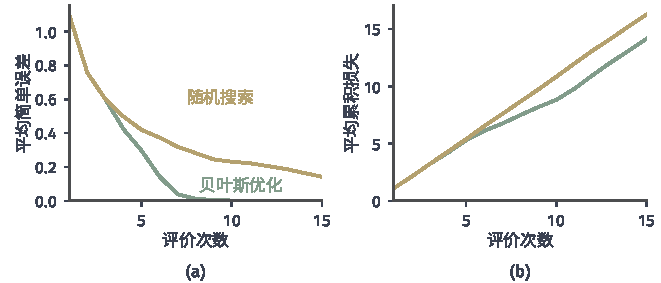
\includegraphics[width=112mm]{figures/05-optimization/05-stochastic-optimization/matplotlib/bo-regret-curves/figure.pdf}
 \caption{贯穿例上的两种误差，$200$组随机初始点的平均值。绿线是贝叶斯优化（$0.1$网格、EI），黄线是均匀随机搜索。(a)当前最好值相对$f^\star$的差；(b)累积损失~\eqref{eq:bo-cumulative-regret}。这是单个一维目标上的教学实验，不代表一般结论。}
 \label{fig:bo-regret-curves}
\end{BookInlineFigure}

\paragraph{不知道$f^\star$时}
贯穿例是人为构造的，$f^\star$可以直接算出。实际问题的最优值未知，就不能直接报告精确的推荐误差，能报告的只有依据明确的比较。可以用已知最优值的基准问题来测方法；可以用有效的下界，比如若$f$是$L$-Lipschitz的，且搜索域中每点到最近评价点的距离不超过$h$，则
\begin{equation}
 f^\star\geq\min_{i\leq T}f(\bm{x}_i)-Lh.
 \label{eq:bo-lipschitz-bound}
\end{equation}
这个不等式成立，因为最小点到某个评价点的距离不超过$h$，函数值的差不超过$Lh$。贯穿例中六个评价点的覆盖半径$h=1.5$，若取$L=2$，下界只有$-4$，松得多，可见这类下界常常只能给出保守的结论。还可以用独立的复核运行来比较候选，这能说明“比基线好多少”，不能说明“离最优多远”。

\subsection{保证的条件}
\label{sec:bo-guarantees}

贝叶斯优化有理论保证吗？可以说有，但条件比较具体。第~\ref{sec:bo-lcb}节留下的问题是：$\kappa_t$取多大，LCB才是有效的置信界？下面的定理针对有限搜索域。

\begin{theorem}[有限搜索域上的同时置信界]
\label{thm:bo-confidence}
设$\bm{C}$是有限集，$f$确实是高斯过程$F$的一个实现，读数噪声是相互独立的$N(0,\tau^2)$，$\tau\geq0$，且每个$\bm{x}_t$只依赖$\mathcal{D}_{t-1}$（可以再用与$F$独立的随机数）。对$\delta\in(0,1)$，令
\begin{equation}
 \beta_t=2\log\frac{\lvert\bm{C}\rvert\pi^2t^2}{6\delta}.
 \label{eq:bo-beta}
\end{equation}
则以至少$1-\delta$的概率，对所有$t\geq1$和所有$\bm{x}\in\bm{C}$，都有
\begin{equation}
 \lvert F(\bm{x})-m_{t-1}(\bm{x})\rvert\leq\sqrt{\beta_t}\,s_{t-1}(\bm{x}).
 \label{eq:bo-confidence}
\end{equation}
\end{theorem}

\begin{proof}
先建立高斯尾的上界。设$W\sim N(0,1)$，$c\geq0$。把积分变量写成$w=c+u$，有
\[
 \phi(c+u)=\phi(u)\,e^{-c^2/2-cu}\leq\phi(u)\,e^{-c^2/2},\qquad u\geq0.
\]
在$u\geq0$上积分，得$\mathbb{P}(W>c)\leq\frac12e^{-c^2/2}$，再由对称性，
\[
 \mathbb{P}(\lvert W\rvert>c)\leq e^{-c^2/2}.
\]

固定$t$和$\bm{x}$。给定$\mathcal{D}_{t-1}$时，$F(\bm{x})$服从$N(m_{t-1}(\bm{x}),s_{t-1}^2(\bm{x}))$。若$s_{t-1}(\bm{x})=0$，不等式~\eqref{eq:bo-confidence}必然成立；否则应用上界，
\[
 \mathbb{P}\bigl(\text{式~\eqref{eq:bo-confidence}对这一组}(t,\bm{x})\text{不成立}\mid\mathcal{D}_{t-1}\bigr)\leq e^{-\beta_t/2}.
\]
这个上界不依赖$\mathcal{D}_{t-1}$，所以对$\mathcal{D}_{t-1}$取期望后仍成立。

对所有$\bm{x}$和所有$t$作并集界。由式~\eqref{eq:bo-beta}，
\[
 e^{-\beta_t/2}=\frac{6\delta}{\lvert\bm{C}\rvert\pi^2t^2},
\]
于是失败概率不超过
\[
 \sum_{t=1}^\infty\sum_{\bm{x}\in\bm{C}}\frac{6\delta}{\lvert\bm{C}\rvert\pi^2t^2}
 =\sum_{t=1}^\infty\frac{6\delta}{\pi^2t^2}=\delta.
\]
最后一步用了$\sum_{t\geq1}1/t^2=\pi^2/6$。
\end{proof}

证明之所以能处理自适应选点，靠的是对每个$t$先以历史为条件，并对$\bm{C}$中全部点取并集，于是不管算法选哪个点，界都成立。代价是系数比单点区间大。$\lvert\bm{C}\rvert=9$，$\delta=0.1$时，
\[
 \sqrt{\beta_1}\approx3.16,\qquad\sqrt{\beta_{10}}\approx4.38,\qquad\sqrt{\beta_{100}}\approx5.33,
\]
都比单点$95\%$区间的$1.96$大得多，且随$t$缓慢增大。

有了同时置信界，LCB的单步损失立刻受控。令$\kappa_t=\sqrt{\beta_t}$，$\bm{x}_t$是$\mathrm{LCB}_{t-1}$的最小点，$\bm{x}^\star$是$f$的最小点。在式~\eqref{eq:bo-confidence}成立的事件上，
\[
 f(\bm{x}_t)\leq m_{t-1}(\bm{x}_t)+\kappa_ts_{t-1}(\bm{x}_t),
\]
而由$\bm{x}_t$的选取，
\[
 m_{t-1}(\bm{x}_t)-\kappa_ts_{t-1}(\bm{x}_t)\leq m_{t-1}(\bm{x}^\star)-\kappa_ts_{t-1}(\bm{x}^\star)\leq f^\star.
\]
两式相减，得到
\begin{equation}
 f(\bm{x}_t)-f^\star\leq2\kappa_ts_{t-1}(\bm{x}_t).
 \label{eq:bo-instant-regret}
\end{equation}
单步损失不超过所选位置的后验标准差的$2\kappa_t$倍，评价的位置不确定性越小，损失越小。

对式~\eqref{eq:bo-instant-regret}求和，再把后验标准差之和联系到\emph{最大信息增益}$\gamma_T$，就得到累积遗憾的上界：若$\tau>0$，$k(\bm{x},\bm{x})\leq1$，上述事件上对所有$T$，
\begin{equation}
 R_T\leq\sqrt{C_1T\beta_T\gamma_T},\qquad C_1=\frac{8}{\log(1+\tau^{-2})},
 \label{eq:bo-regret-bound}
\end{equation}
其中$\gamma_T$是在$T$个点上观测所能获得的最大信息增益。这一步的证明需要用到高斯信息量的链式分解和方差的求和估计，篇幅较长，读者可查阅GP-UCB方法的原始分析。对平方指数核和紧凸搜索域，$\gamma_T$随$T$只按$\log T$的多项式增长，所以$R_T/T\to0$。

这个结论的适用范围要说清楚。它要求$f$确实由所用的高斯过程产生、核和噪声方差已知、内层问题精确求解、搜索域有限；连续域需要额外的光滑性条件和离散化论证。它只对这种特定的GP置信界方法成立，不覆盖任意代理与采集函数的组合。常用的EI加上每轮重新估计超参数，就不在这个定理的范围内，模型失配和内层求解误差也都要另外检查。

表~\ref{tab:bo-claims}把几种容易混淆的说法分开。

\begin{BookInlineTable}
 \centering
 \caption{三种不同的主张。}
 \label{tab:bo-claims}
 \begin{tabular}{ll}
 \toprule
 主张&需要的条件\\
 \midrule
 单点后验可信区间&模型正确，点在观测前固定\\
 自适应的同时置信界&模型正确，并集界，系数随$t$增大\\
 有限预算找到全局最优&一般不成立，需要对$f$作额外假设\\
 \bottomrule
 \end{tabular}
\end{BookInlineTable}

最后一行值得多说一句。有限次评价只能在有限个点取值，两个点之间函数可以任意低，除非另有光滑性之类的假设，否则任何算法都不能保证找到全局最优。这也是概率模型的角色所在：它把这种假设明确写了出来，让我们知道结论依赖什么。

\section{本章小结}
\label{sec:bo-summary}

本章的出发点是预算极少的黑箱问题，$T$次评价要在有希望的区域和未知的区域之间分配。评价点负责收集信息，推荐解负责交付，选点规则只能使用已完成的观测。目标本身并不随机，概率描述的是我们对它的认识。

概率代理把已完成的观测变成对所有候选位置的预测。高斯过程用核表达“相近的位置函数值相近”，一个读数通过后验协方差影响相关的位置，后验方差只取决于评价放在哪里。超参数不确定时，直接代入估计值可能严重低估不确定性，低方差只说明在模型内不确定性小。

采集函数把预测变成分数：PI只看过线的概率，EI把幅度也计入，LCB直接按乐观值比较，Thompson采样按后验抽样选点，KG衡量一次观测对最终推荐的改善。四种规则的共同之处是都在利用与探索之间折中，不同之处在于如何折中。循环的外层是昂贵评价，内层是对采集函数的优化，而内层的求解质量也影响选点。

各种推广分别改变了循环的某一环。噪声改变了阈值的含义，需要区分潜在函数值和下一次读数，复测的价值要由信息更新的准则衡量。约束在采集分数中加入可行概率，$b_t$也改为可行读数中的最好值；要求每次试验都可行时，还需要额外的安全假设。并行使一批候选之间的相关性变得重要，未完成的试验要按预测分布平均，而不当作已有读数。成本则改变了预算的口径。

最后要分开三件事：模型给出的概率是否可信，优化的结果是否够好，计算的开销是否值得。特定的GP置信界方法有遗憾上界，但它依赖模型正确、搜索域有限和置信系数的具体取值；这些条件不满足时，算法仍可以使用，只是结论要靠实际的对照比较来支持。


